%
%  RAL XFEL FEE CCC/ASIC interface manual
%
%  Created by Sam Cook on Mon 28 Jan 2013
%
%  Copyright (c) 2013 RAL. All rights reserved.
%
\documentclass[12pt]{book}

% Use utf-8 encoding for foreign characters
\usepackage[utf8]{inputenc}

% Setup for fullpage use
\usepackage{fullpage}

% Uncomment some of the following if you use the features
%
% Running Headers and footers
%\usepackage{fancyhdr}

% Multipart figures
%\usepackage{subfigure}

% Multirow tables
\usepackage{multirow}

% More symbols
\usepackage{amsmath}
\usepackage{amssymb}
\usepackage{wasysym}
\usepackage{latexsym}

% Surround parts of graphics with box
% \usepackage{boxedminipage}

% Stop the float madness! doesn't seem to work, stick with htbp
% \usepackage{float} 

% Package for including code in the document
\usepackage{listings}

% Package for including code in the document
\usepackage{minted}
% If you want to generate a toc for each chapter (use with book)
\usepackage{minitoc}

% This is now the recommended way for checking for PDFLaTeX:
\usepackage{ifpdf}

% Add a bit of extra height to tables so '\hlines' don't look crap
\usepackage{array}
\setlength{\extrarowheight}{1.5pt}
% Specify a new column type 'X' that is fixed width and centred
% \newcolumntype{X}[1]{>{\centering\let\newline\\\arraybackslash\hspace{0pt} } p{#1} }
\newcolumntype{X}[1]{>{\centering\let\newline\\\arraybackslash\hspace{0pt}}m{#1}}
% This gives better decimel place alignment (apparently)
% Still needs multicolumns in the header to align correctly
\usepackage{dcolumn}
% Arguments are:
% D<column sep (instead of &)><column sep to insert><n decimal places>
\newcolumntype{d}[1]{D{.}{.}{#1}}

% Set footnotes to be symbols as it stops random powers appearing
\renewcommand{\thefootnote}{\fnsymbol{footnote}}
% Reset the footnote 'counter' every page
\usepackage{perpage} %the perpage package
\MakePerPage{footnote} %the perpage package command

% Create tables of a defined total width with wrapped columns
\usepackage{tabulary}
% threeparttable gives us access to footnotes in tables
\usepackage{threeparttable}
% wan to get ditto mark
\usepackage[T1]{fontenc}
\newcommand*{\dittostraight}{---\textquotedbl---} % available in T1 encoding

% We want a nice tick & cross symbol for comparison tables
\usepackage{pifont} 
\newcommand{\cmark}{\ding{51}}%
\newcommand{\xmark}{\ding{55}}%
\newcommand{\mus}{$~\mu$s}

% make bullet point lists with tighter spacing
\usepackage{mdwlist}
%\newif\ifpdf
%\ifx\pdfoutput\undefined
%\pdffalse % we are not running PDFLaTeX
%\else
%\pdfoutput=1 % we are running PDFLaTeX
%\pdftrue
%\fi

% rotating also includes graphicx so don't double import (causes error)
\ifpdf
\usepackage[pdftex]{graphicx}
\else
\usepackage{graphicx}
\fi

% Allow full page landscape images
\usepackage{rotating}


% lineup from jpconf
\def\lineup{\def\0{\hbox{\phantom{0}}}%
    \def\.{\hbox{$\phantom{.}$}}%
    \def\m{\hbox{$\phantom{-}$}}%
    \def\-{\llap{$-$}}}

% TODO ACTUAL TITLE!
\title{Characterisation of the MuSIC muon beam.}
\author{ Sam Cook }

\date{\today}
\graphicspath{{4_appendix_XFEL/}{1_introduction/}{3_measurements/}{2_simulation/}}
\renewcommand{\sfdefault}{phv}
\begin{document}    

    \maketitle
    \tableofcontents
    \chapter*{Preface} % (fold)
\label{cha:preface}
This thesis is divided into two parts. The first part covers work done at the Muon Science Innovative Channel (MuSIC) beam-line and the second part, an appendix, discusses some work carried out on the European X-ray Free Electron Laser (EuXFEL).

The first part, discussing MuSIC, has two main themes: simulation and measurement. An introduction (chapter~\ref{prt:introduction}) covers the essentials of the project and the physics behind it. Chapter~\ref{prt:simulation} describes the development of the MuSIC simulation  and its deployment in creating a rigorous analysis. Finally chapter~\ref{prt:measurement} discusses the results of the measurements made at MuSIC.

The second part is concerned with creation of the firmware interface between the Clock and Control Card (CCC) and the Large Pixel Detector (LPD). It discusses the design, implementation and testing of the firmware ahead of use in EuXFEL.

\chapter{Executive Summary} % (fold)
\label{cha:executive_summary}
The Muon Science Innovative Commission (MuSIC) beam line is a prototype muon production system being developed at the Research Centre for Nuclear Physics (RCNP) in Osaka, Japan. It uses a novel Pion Capture Solenoid (PCS) that captures a much larger fraction of the produced pions than other muon beam lines do. Once the pions have been captured they are directed in to the Muon Transport Solenoid (MTS) where they can decay to produce muons. MuSIC aims to achieve a muon production efficiency (per Watt of proton beam) that is far higher than is currently seen at existing beam lines. 

High flux, low power muon beams will enable the creation of dedicated muon Spin Resonance (\(\mu\)SR) devices, they are a first step in making neutrino factories as well as being vital in particle physics studies such as the measurement of rare decays (e.g.\ \(\mu\rightarrow eee\)). In addition to research muon beams can be used in the development of other technologies, e.g.\ MuSIC will be used to conduct research into Fixed Field Alternating Gradient (FFAG) storage rings and test their viability as an acceleration technology for muons.

A key use of MuSIC will be as a prototype for the Coherent Muon-to-Electron Transition (CoMET) experiment being planned to be built at J-PARC in Tokai, Japan. CoMET will use a similar, albeit larger, pion capture solenoid to produce a pulsed beam of \(10^{11}\)~muons~s\(^{-1}\) that will enable it to make the most precise measurements of the rare muon decay: \(\mu X\rightarrow eX\). The insights gained at MuSIC, both in terms of the technology and the science, will help improve the measurements made at CoMET. 

In order to better understand MuSIC it was simulated using Geant4 and G4Beamline (G4BL). Two core simulations were made, one of the PCS and MTS made using G4BL and a second of the detectors made using Geant4. The G4BL simulation was used to test the initial designs of MuSIC and later to provide realistic particle distributions for the Geant4 simulation. The detector simulation, made in Geant4, was used to test detector configurations and refine analysis techniques.

Commissioning of the PCS and the first 36\(^{\circ}\) of the MTS was completed in 2010. The final design of MuSIC has a planned 180\(^{\circ}\) MTS but there is enough to begin characterising the beam. Over two years there were five periods of beam time, each lasting between 24 and 72 hours, for which the RCNP's proton beam was available for use at MuSIC. 

During the five beam times detectors and data acquisition (DAQ) were installed, tested and used to make three different measurements that help characterise the MuSIC beam. The three measurements were of the total charged particle flux, the muon lifetime and the muon momentum spectrum. Each experiment used simple detectors made of plastic scintillators with Multi-Photon Pixel Counters (MPPC) for read out. 

The charged particle flux was measured in two separate beam times, firstly with a long strip scintillator (1\(\times\)3\(\times\)38~cm) and then with a disk scintillator (3.5\(\times\)2~cm). The first measurement was made 6~cm from the end of the MTS at a range of heights. The peak charged particle flux was measured to be (94.3\(\pm\)4.0)\(\times10^3\)~particles~nA\(^{-1}\) at \(5\)~cm above the beam pipe's centre. The second measurement was made 85~cm from the end of the beam pipe at range of horizontal and vertical positions. The peak flux for the second measurement was (11.16\(\pm\)0.11)\(\times10^3\)~particles~nA\(^{-1}\) at \((0, 20)\)~cm, i.e.\ directly above the beam pipe's centre. The second most intense location was at \((-17, 0)\)~cm, to the left of the beam centre (when facing it). Both these measurements show that the most intense part of the beam is above the centre and the second also shows that the this spot is slightly offset towards the left, which agrees with the simulation although not on the predicted intensity.

The muon lifetime was measured during two beam runs as a method of demonstrating the presence of muons in the beam. The measurement was made by using two scintillators on either side of a metal stopping target. By plotting the time between events in each scintillator the muon decay spectrum could be constructed and the muon's lifetime measured. The first measurement of the muon lifetime was made during the same beam time as the second charged particle measurement and recorded a lifetime of (2,016\(\pm\)88.6)~ns which is lower than the canonical value of (2,196.9811\()\pm\)0.0022)~ns~\cite{pdg} although this is likely due to the presence of a stopping target which would have reduced the negative muon's lifetime. The second measurement attempted to account for the presence of the stopping target by fitting the muon lifetime with two exponentials and hence measured the free muon lifetime to be (2,202\(\pm\)20)~ns and the lifetime of negative muons in the copper stopping target to be (195\(\pm\)17)~ns. The lifetime of muonic copper was slightly higher than the canonical value of (163.5\(\pm\)1)~ns measured in by Suzuki~et~al.~\cite{suzuki_mu_capture_rates} but is still reasonable.

The final measurement, the muon momentum spectrum, was the most complex. Six measurements were made using one of four different thickness aluminium degraders. The degraders reduced the energy of any charged particles and so filtered out different momentums to stop on the copper stopping target. By plotting the decay spectrum and integrating the area under the exponential portion it was then possible to count the number of stopped muons and hence estimate the number of muons of that momentum. The momentum spectrum measured for freely decaying muons is shown in figure~\ref{fig:exec_summary_muon_momentum_spectrum}. This figure also shows the reasonable agreement between the simulation and the measurement although the errors on the measurement obviously need improvement. 

\begin{figure}[htpb]
  \centering
    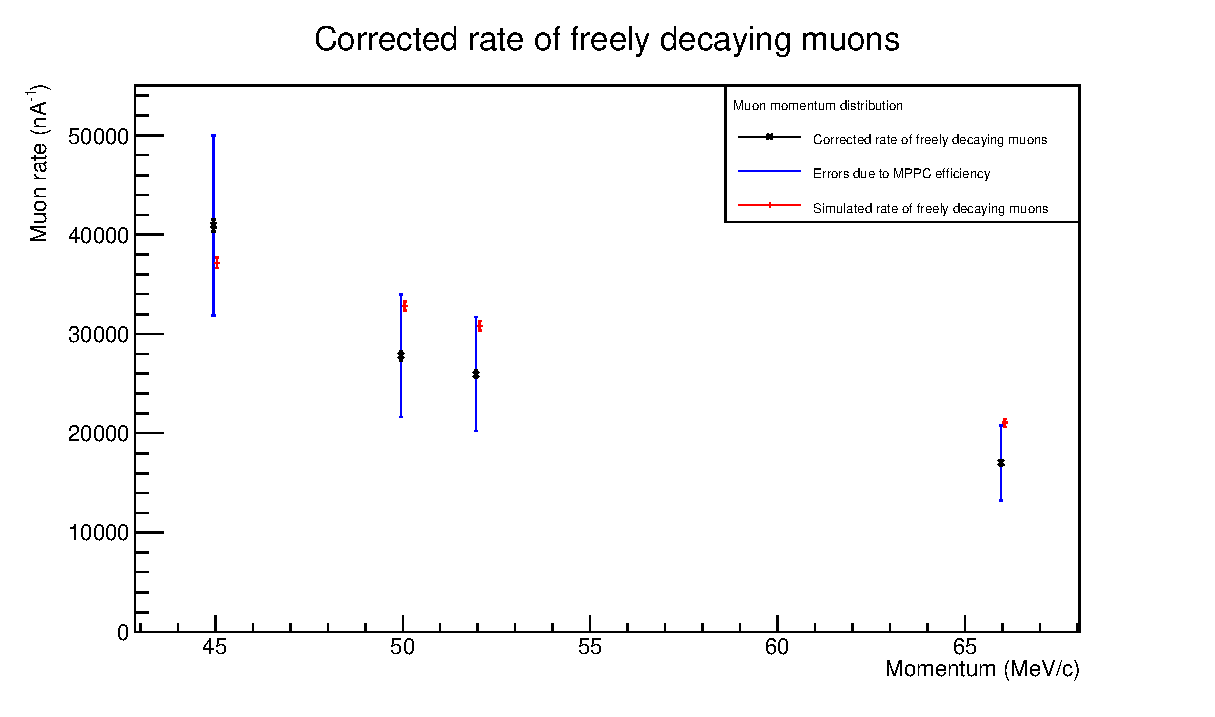
\includegraphics[width=.9\textwidth]{../3_measurements/images/plot_generating_scripts/adjusted_muon_rates.eps}
  \caption{Muon momentum spectrum for freely decaying muons.}
  \label{fig:exec_summary_muon_momentum_spectrum}
\end{figure}

Using the data from the momentum spectrum measurement it was possible to predict the total muon flux at MuSIC when operated at full power\footnote{To prevent excessive dead time in the equipment currents of \(<\)1~nA were used rather than the RCNP's maximum current of 1~\(\mu\)A.} and this was calculated to be \((4.16\pm0.53)\times10^8\)~muons~s\(^{-1}\) which is on par with the world's most intense muon source, PSI, which has a peak flux of \(4.8\times10^8\)~muons~s\(^{-1}\). The key difference between MuSIC and PSI is that PSI produces its muons using a 1.2~MW proton beam compared to the RCNP's 400~W beam, giving per-Watt efficacies of \((8.3\pm1.1)\times10^5\)~muons~W\(^{-1}\) and 292~muons~W\(^{-1}\) respectively.

% chapter preface (end)
%%%%%%%%%%%%%%%%%%%%%%%%%%%%%%%%%%%%%%%%%%%%%%%%%%%
\chapter{Introduction} % (fold)
\label{prt:introduction}
MuSIC is a new muon source housed at the Research Centre for Nuclear Physics (RCNP) in Osaka, Japan. Commissioning of the beam began in 2010 with installation of the Pion Capture System (PCS) and the first 36\(^{\circ}\), of a planned 180\(^{\circ}\), of Muon Transport Solenoid (MTS). To date there have been five periods of beam time.

Over the course of the five sessions of beam time three core measurements have been made that will be discussed in this thesis:
\begin{enumerate}
  \item Charged particle flux.
  \item Muon lifetime.
  \item Muon momentum spectrum.
\end{enumerate}
All of these experiments have had the aim of characterising the beam at MuSIC and confirming the efficiency of muon production. The measurements themselves are discussed in chapter~\ref{prt:measurements}.

While still incomplete, enough of MuSIC exists to test the efficacy of the PCS and existing MTS. The PCS uses a novel design in order to to maximise muon production. This new design is predicted to be several orders of magnitude more efficient than current methods.

The rest of this chapter is divide into three sections: Muon sources (section~\ref{cha:high_intensity_muon_sources}), MuSIC (section~\ref{cha:music}) and physics (section~\ref{cha:physics}). `Muon sources' discusses existing muon beams and goes on to make the case for high intensity muon sources. The section on MuSIC discusses its design and the scientific motivation for building it. Finally the physics section reviews the theory behind charged particle interactions in matter, muon decay and charged Lepton Flavour Violation (cLFV).

\section{Muon Sources} % (fold)
\label{cha:high_intensity_muon_sources}
The muon was the fist second-generation particle to be discovered, it has been used to test the theory of relativity~\cite{rossi_hall_first_muons}, measure the size of the proton~\cite{proton_size} and to measure oscillations of neutrinos~\cite{t2k_cdr}. Not only is the muon an interesting particle in its own right, but a powerful and precise tool of further research. 

Muons are a lepton; they are \(\sim\)200 times more massive than their sibling, the electron\footnote{The mass of the muon is 105.6583715\(\pm\)0.0000035~MeV, an electron is \( 510.998928\pm0.000011 \)~keV~\cite{pdg}.}. Unlike the electron muons can decay and majority of the time\footnote{\(\approx100\%\) of the time~\cite{pdg}.} muons decay via the process \(\mu\rightarrow e\nu\overline{\nu}\), the muon's lifetime prior to undergoing decay is 2.1969811\( \pm \)0.0000022~\( \mu \)s~\cite{pdg}. Muons interact via the electroweak forces and are, as far as we know, elementary particles.

More than any other property, the lifetime of the muon, encompass the biggest problem with muon sources. The fact that muons decay; unlike protons, neutrons\footnote{The neutron's lifetime is \(880.0\pm0.9\)~s~\cite{pdg} enough to make it stable in comparison to the muon.} and electrons, makes manipulating muons a race against time. All beams have similar stages: production, acceleration, cleaning and finally deployment; for muons this has to happen in the 2.2\(\mu\)s that the muons exist for. Despite the difficulty of creating muon beams the usefulness of a non-electron lepton beam is not to be underestimated.

As a particle that isn't common in nature muons cannot be produced in the same way as, e.g.\ electrons: via ionisation and subsequent acceleration. The most common method for muon production is via pion decay (see figure~\ref{fig:pion_decay_feyman}), this process has a branching ratio of 99.98770$\pm$0.00004~\%~\cite{pdg}\footnote{The next most common decays are \( \pi\rightarrow\mu\nu_{\mu}\gamma \) and \( \pi\rightarrow e \nu_e \) which have branching ratios of \( (2.00\pm0.25)\times10^{-4} \)\% and \( (1.230\pm0.004)\times10^{-4} \)\% respectively.}. The pion has a lifetime of only 26.033\(\pm\)0.005~ns~\cite{pdg}, i.e.\ \( \sim \)1\% of the lifetime of the muon meaning that given a suitable amount of time, the pion contamination of the muon beam can be kept low. Pion production is occurs through proton-proton interactions above the energy threshold of \( \sim380 \)~MeV. The simplest method achieving proton-proton interactions above the pion production threshold is through the bombardment of a fixed target with a proton beam.

\begin{figure}[hptb]
  \centering  
    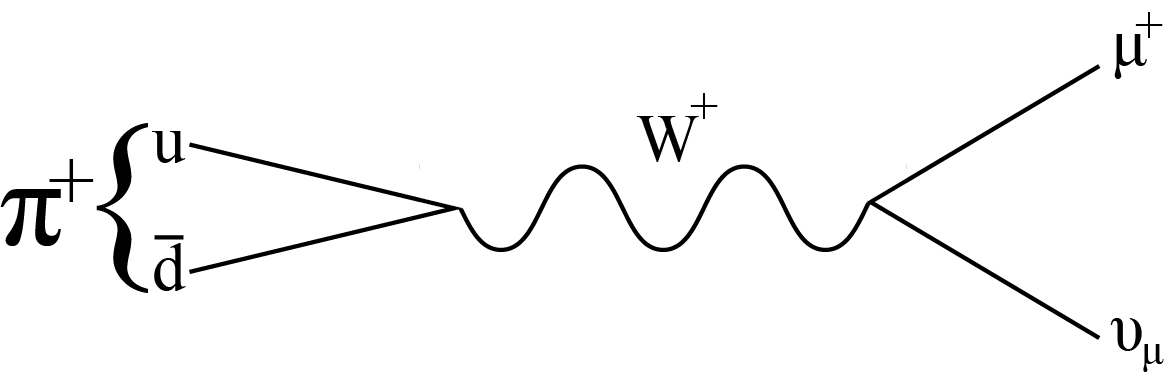
\includegraphics[scale=0.8]{images/pion_decay_feyman.png}
  \caption{Feynman diagram showing muon production through pion decay.}
  \label{fig:pion_decay_feyman}
\end{figure}

Whilst all muon sources use pion decays to generate their beams there are several broad categories of beam. Muon beams are generally categorised depending on where the muons originate: `cloud', `surface' and `sub-surface'. Most muon facilities will have one or more of each type of beam, as they are not incompatible and all have different properties. `Cloud' beams collect pions (and some muons) then transport them to a `decay pipe' in which the remainder of the pions can decay. In general cloud type beams with have a larger range of momenta as the pions decay in flight. `Surface' and `sub-surface' beams are both generally of lower momenta (\( <30\)~MeV/c) than cloud types as they collect muons produced by pions decaying at rest on (or just inside) the surface of the target. Surface and sub-surface beams are in high demand for muon Spin Resonance (\(\mu\)SR, see section~\ref{sub:muon_spin_resonance}) experiments which require high fluxes of low momentum muons.

There are currently several dedicated muon sources\footnote{In theory any proton source, with energy above the pion production threshold, can operate as a muon source but only a few have dedicated facilities.} around the world (see table~\ref{tab:cf_muon_sources}). All of the current muon sources have their facilities acting in a parasitic mode on their main proton beam-line, with the majority of the proton beam being used for neutron sources. Most muon facilities have several separate beam-lines that can operate semi-independently, with each beam-line often specialising in a certain sub-set of muons. For example, RIKEN-RAL has 4 experimental ports: port-1 is used to investigate muon-catalyzed d-t fusion (\(\mu\)CF), port-2 and port-4 are dedicated \(\mu\)SR experiments; and port-3 is used for low energy muon production.

\begin{table}[htpb]
  \begin{center}
  \begin{tabular}{c | c | c | c | c | c | c}
    Name       &  \multicolumn{3}{c|}{Muon beam}                 &  \multicolumn{2}{c|}{Proton Beam}  &   Ref \\
               &  Flux (muons/s)     &  Type  & \( P \) (MeV/c)  &  Power (W)    & \(I\) (\(\mu\)A)   &       \\
    \hline    
    PSI        &  \(4.8\times10^8\)  &  Cont.  &  28  &  \(1.2\times10^6\)  &  2000  &  \cite{mue4_psi}   \\ 
    RIKEN-RAL  &  \(6\times10^5\)    &  Pulse  &  27  &  \(1.6\times10^3\)  &  200   &  \cite{riken_ral}       \\
    TRIUMF     &  \(3.5\times10^6\)  &  Pulse  &  25--85  &  \(7.0\times10^4\)  &  140   &  \cite{triumf_m20a} \\
  \end{tabular}
  \end{center}
  \caption{Comparison of several leading muon sources. As most sources have multiple muon beam-lines the highest flux station at each source was chosen: \(\mu\)E4 at PSI; port-1 of the RIKEN-RAL facility and the M20A beam-line at TRIUMF. The difference in momenta is due to both \(\mu\)E4 and port-1 using surface muons whilst M20A uses cloud muons. Beam type refers to whether the beam is continuous or pulsed. \( P \) is the muon momentum (either as an average if reasonably mono-energetic or a range), \( I \) is the proton beam's current.}
  \label{tab:cf_muon_sources}
\end{table}


\subsection{Scientific Motivation for High Intensity Muon Sources} % (fold)
\label{sec:scientific_motivation_for_high_intenstity_muon_sources}
As has been noted muons are highly active area of research, both as a tool for further research and a focus of study. The activity surrounding muon beams is only increasing as new technologies become available and our ability to control these short lived beams increases. 

As a focus for study, in and of themselves, muons present several interesting avenues for research. Muons are a well understood particle who's interactions are known to high precision. Because muons are so well understood they make an excellent arena to test the limits of our knowledge: by making precision measurements of the muon and its interactions we can test regions of theory that are otherwise inaccessible. For example, by looking for charged Lepton Flavour Violating (cLFV, see section~\ref{sec:charged_lepton_flavour_violation}). Through cLFV processes such as \( \mu\rightarrow eee \) or \( \mu N \rightarrow N^* e \), we can test the limits on many `beyond the standard model' theories. Obviously, in order to measure a process that has, so far, never been seen you need an ample supply of the source material so high intensity muon sources are vital for these measurements.

Currently one of the most active areas of research in particle physics is that of neutrinos. Whilst very common in nature the neutrino's tiny cross section makes study of it very difficult. In recent years this has been solved through the creation of neutrino beams such as T2K~\cite{t2k_cdr}. Neutrino beams are normally created using the decay products of pions but there is growing interest in building so-called `neutrino factories'. One proposed design for a neutrino factory uses an oval storage ring to hold muons until they decay to create a mixed electron/muon-neutrino beam, obviously if many more neutrinos are wanted then then significantly higher intensity muon sources are needed.

A commonly described evolution of the neutrino beam is to create a second muon beam and counter rotate them in order to produce a muon collider. A leptonic collider is highly attractive: as an elementary particle collisions are cleaner and can be more finely controlled whilst the higher mass of the muon over the electron means that there is much less energy loss to synchrotron radiation. A muon collider would present many challenges but with the International Linear Collider (which uses electrons) expected to be \(\sim\)31~km long~\cite{ilc} smaller, more complex, colliders become better options. If a muon collider can be built as the next stage of a neutrino factory, so much the better.

Particle physics presents just one facet of the many uses to which muon beams can be put. One of the most common uses of muon beams is probing the magnetic properties of materials through \(\mu\)SR, other applications include using muons to determine the nuclear matrix elements of materials, measuring trace elements in a sample through the emission of muonic X-rays and research into \(\mu\)CF.

% section scientific_motivation (end)
%%%%%%%%%%%%%%%%%%%%%%%%%%%%%%%%%%%%%%%%%%%%%%%%%%%
% chapter high_intensity_muon_sources (end)
%%%%%%%%%%%%%%%%%%%%%%%%%%%%%%%%%%%%%%%%%%%%%%%%%%%
\section{MuSIC} % (fold)
\label{cha:music}
% TODO Introduction: MuSIC Obligatory pictures of final design of MuSIC & current status
MuSIC is a proof of concept beam-line that aims to produce the most muons per proton of any existing source. MuSIC aims to have a muon flux comparable to that of PSI's (the current world best) using a beam with \(^1/_{3,000}\) the power. This can be done by one of two naive methods: increasing the efficiency of production or using a more powerful initial beam. At both RIKEN-RAL and PSI the muon beams are produced using only a fraction of the initial proton beam. It is common that less than 10\% of the initial proton beam is used to create muons, the rest continues to neutron sources. Obviously to create a high intensity muon beam using as many of the protons as possible should be the first design goal. There is a second advantage to moving away from a parasitic muon production: not only is the entire proton beam used but more of the pions can be captured. In a parasitic design the PCS has to allow the for the continuation of the proton beam, this places limits on the geometry that can be used and produced sub-optimal efficiencies. If the requirements for a continuing proton beam are removed though, the PCS geometry can be optimised purely for pion capture making further gains over merely increasing the proton current.

\begin{figure}[htbp]
  \centering
    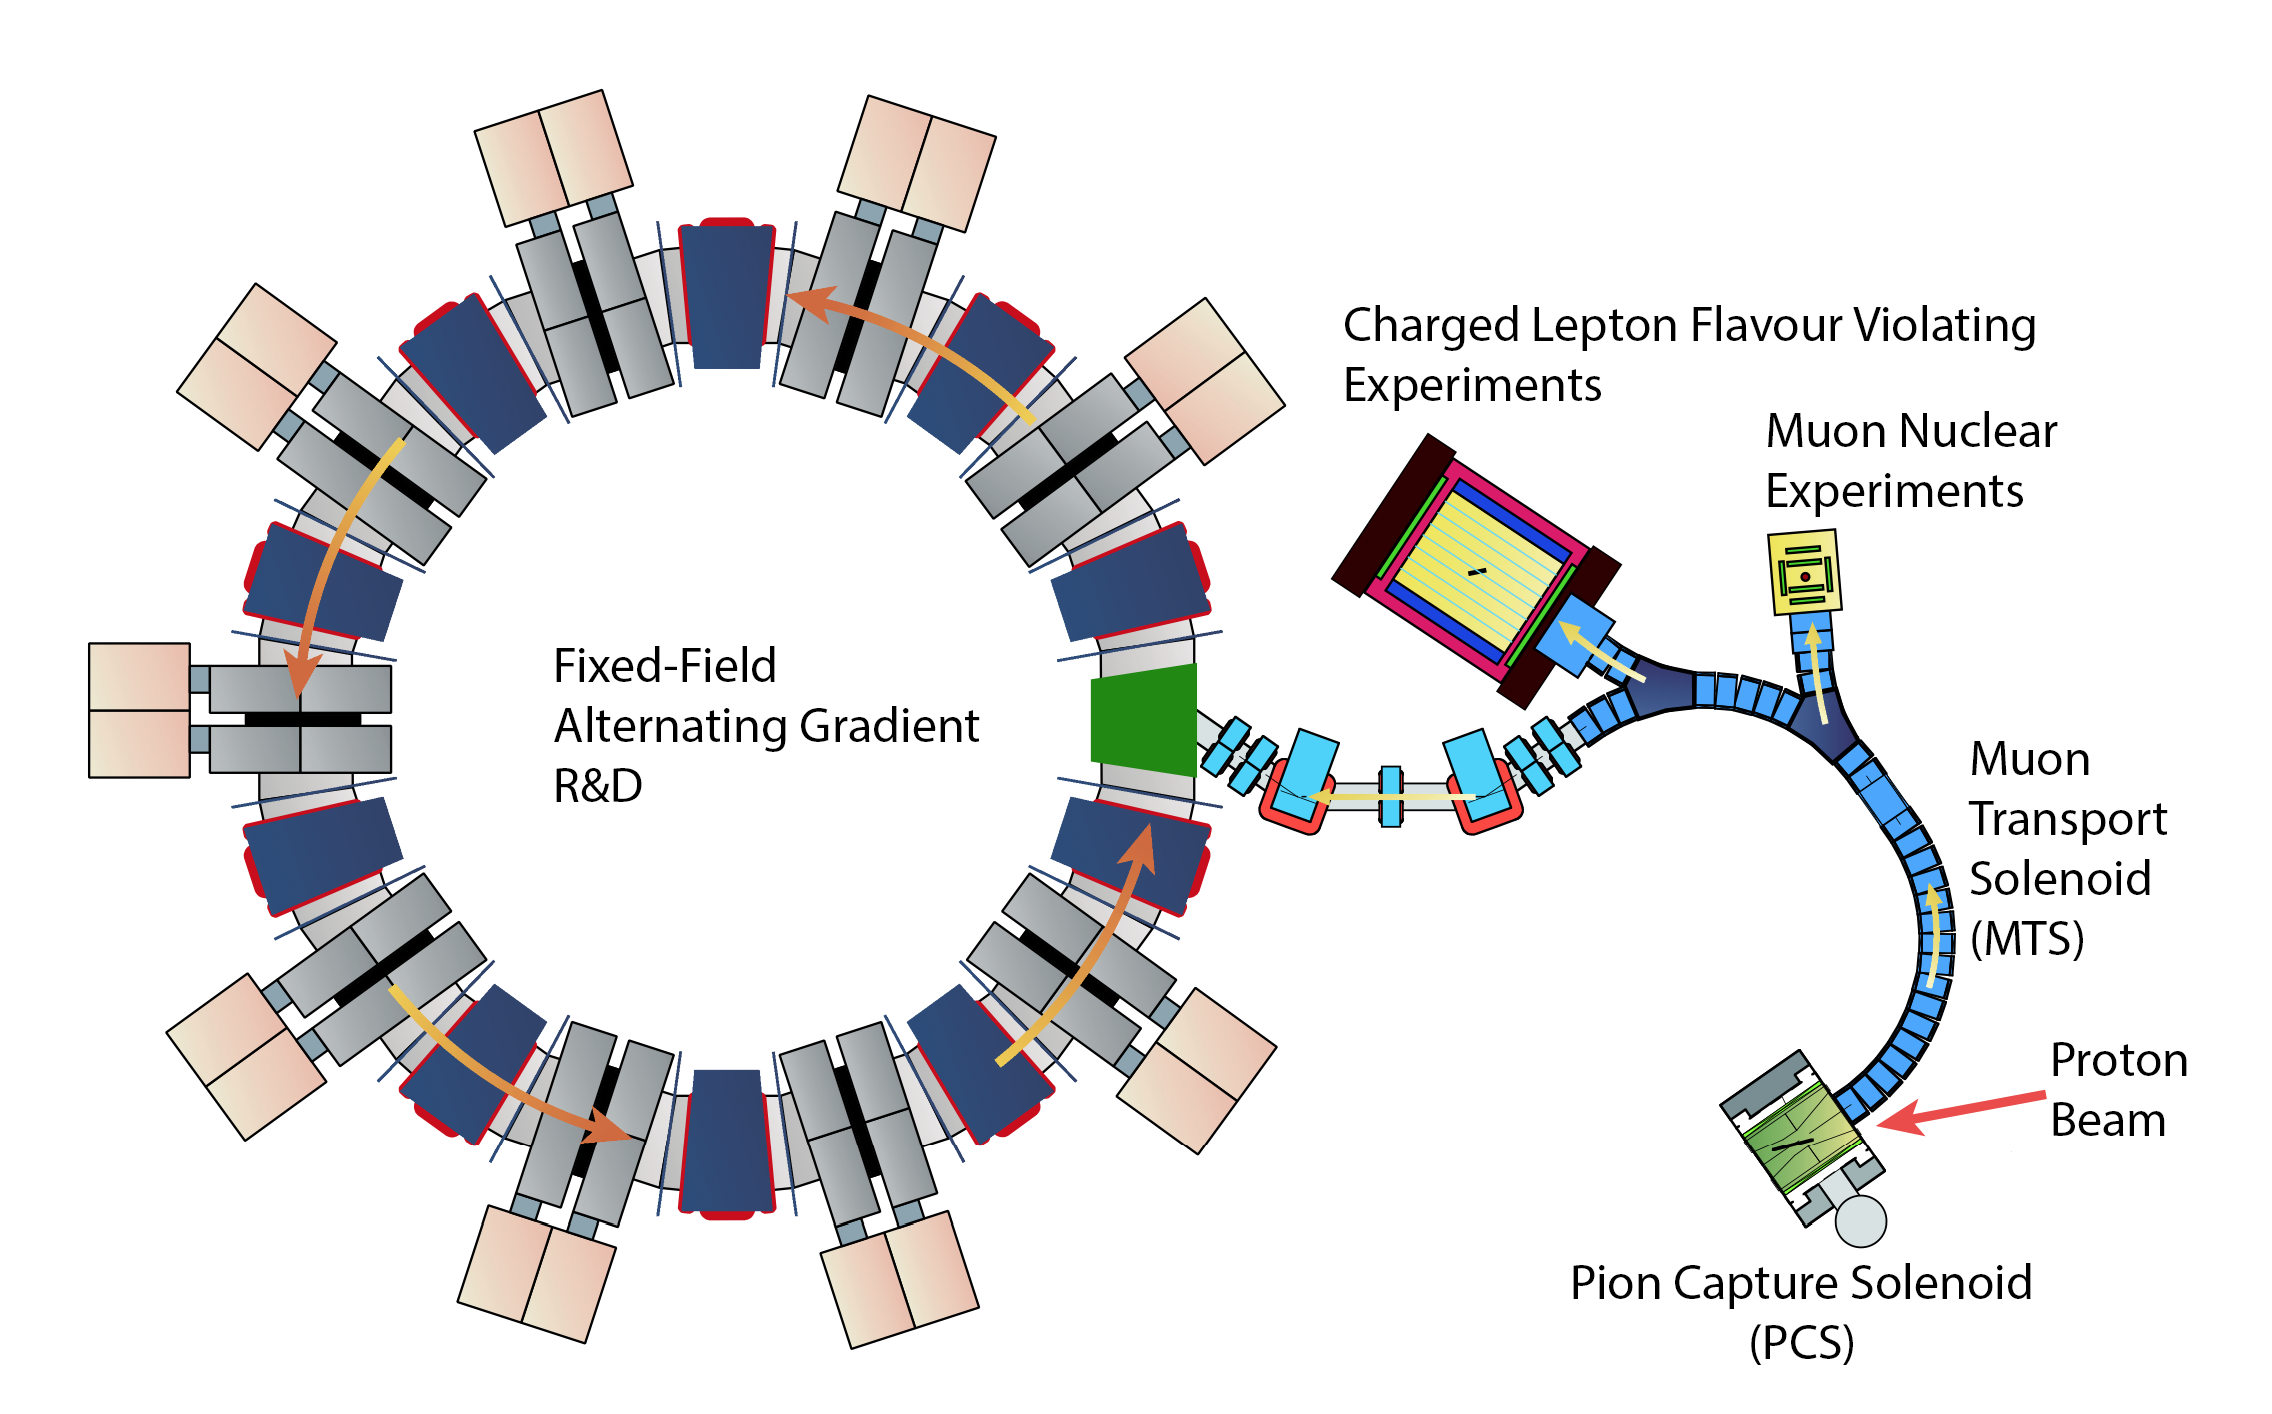
\includegraphics[width=.9\textwidth]{images/MuSIC_schematic_FFAG.png}
  \caption{Schematic of the completed MuSIC complex.}
  \label{fig:images_MuSIC_schematic_FFAG}
\end{figure}

\begin{figure}[htbp]
  \centering
    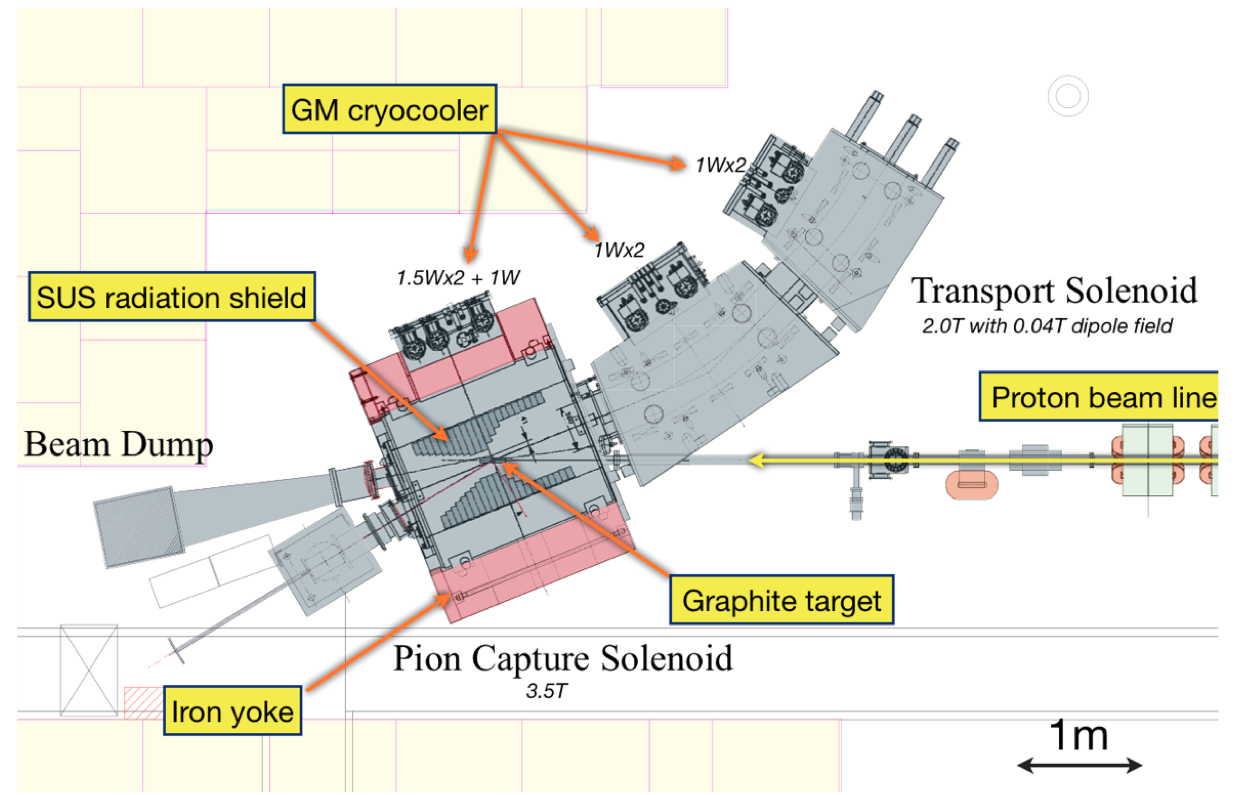
\includegraphics[width=.9\textwidth]{images/MuSIC_current_schematic.png}
  \caption{Schematic of the current status of MuSIC.}
  \label{fig:images_MuSIC_current_schematic}
\end{figure}
\begin{figure}[htbp]
  \centering
    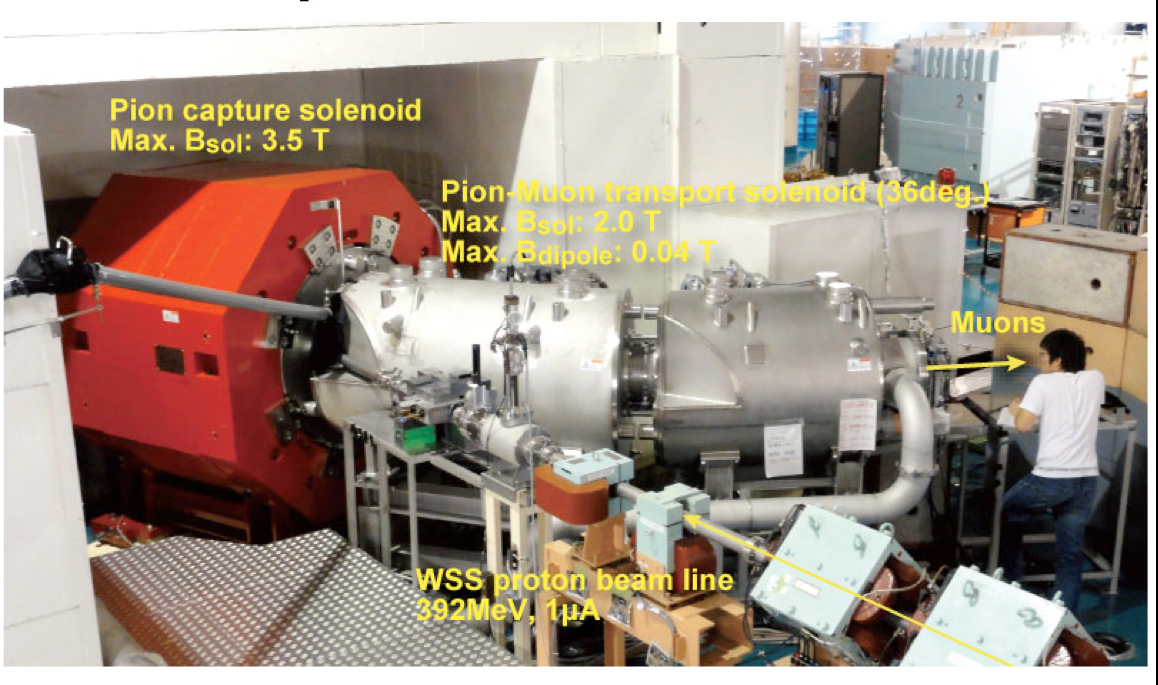
\includegraphics[width=.9\textwidth]{images/MuSIC_photo.png}
  \caption{Photo of MuSIC showing its 2010 status, since then it has had further concrete blocks added around it to increase shielding.}
  \label{fig:images_MuSIC_photo}
\end{figure}

Figure~\ref{fig:images_MuSIC_schematic_FFAG} shows the completed MuSIC complex including the proposed experimental stations, compare this to the schematic in  figure~\ref{fig:images_MuSIC_current_schematic} which shows the current status, with the Pion Capture System (PCS) and the first 36\(^{\circ}\) of Muon Transport Solenoid (MTS) complete, figure~\ref{fig:images_MuSIC_photo} is a photo of the status of MuSIC in 2010, prior to the addition of further shielding.

\subsection{MuSIC design} % (fold)
\label{sec:music_design}
The core component of MuSIC is its PCS. The MuSIC PCS is designed to use as much of the proton beam and capture as many pions as possible. The PCS achieves this with a \(2.1\times2.4\times1.6\)~m\(^3\) super-conducting magnet that has a maximum strength of 3.5~T. The PCS has an extremely large solid angle making MuSIC capable of capturing a significant portion of the pions and directing them into the muon transport solenoid (MTS).

The MTS is intended to perform three roles within MuSIC: the collection and decay of travelling pions; selection of low-energy (30--50~MeV) muons and selection of muon charge. Ultimately the MTS will form a 180\(^{\circ}\) semi-circle but currently only the first 36\(^{\circ}\) has been constructed. The MTS's designed 10m length provides the requirements for pion decay; its radius and magnetic field provide momentum selection whilst the application of a dipole field will select charge. Like the PCS the MTS uses super-conducting magnets to provide the 2~T main field and the 0.04~T dipole field.

The proton beam for MuSIC is provided by the RCNP's ring cyclotron. The cyclotron produces a 400~MeV proton beam (enough for pion production) with a maximum current of \( 1\mu \)A giving a maximum power of 400~W. The beam is produced in an ion source then accelerated using two cyclotrons: the AVF and then the ring cyclotron. The first cyclotron, AVF, can accelerate a variety of ions (up to \(^{18}\)O) using a voltage of 60~kV, for protons this corresponds to a final energy of \(\sim\)65~MeV. The ring cyclotron then accelerates the protons to \( \sim \)400~MeV. 

The MuSIC PCS has been optimised to capture backwards travelling pions and muons with a maximum transverse momentum (\(P_{T}^{max}\)) of 52.5~MeV. The two key parameters that determine \(P_{T}^{max}\) are the magnet's bore and the field strength, through optimisation these were determined to have values 10~cm and 3.5~T respectively. To obtain a 3.5~T field copper-stabilized NbTi superconductor was used, this requires cooling to 4~K which is achieved through the use of 3~GM cryocoolers. 

The target used is a graphite cylinder 20~cm long with a 2~cm radius. To maximise production the target is rotated from the PCS axis to align its major axis with the proton beam. The superconducting magnet is shielded using stainless steel that has a maximum thickness of 27~cm, the shielding tapers on either side of the target (see figure~\ref{fig:images_MuSIC_current_schematic}). The taper is more rapid in the backwards direction in order to capture the maximum number of pions and muons.  

As already noted the muon transport solenoid (MTS) has to select muon momentum and charge whilst letting pions decay. The MTS has a designed length of 10~m which is predicted to reduce the pion contamination to less than 0.1\%. Application of the dipole field can be used to select charge.

% section music_design (end)
%%%%%%%%%%%%%%%%%%%%%%%%%%%%%%%%%%%%%%%%%%%%%%%%%%%
\subsection{MuSIC: Scientific Motivation} % (fold)
\label{sec:music_scientific_motivation}
The general arguments for high intensity muons beams have already been presented (section~\ref{sec:scientific_motivation_for_high_intenstity_muon_sources}), MuSIC, though is not technically a high intensity muon beam. Assuming that it meets full design specifications it should have a comparable intensity to the muon beam-lines at PSI. To this end the scientific case for MuSIC is slightly different to that for a full high intensity muon beam. The key aim of MuSIC is in proving the PCS and MTS technology, what PSI achieves with a 1.3~MW proton beam MuSIC aims to achieve with a 400~W beam. This section will set out the other uses to which MuSIC will be put.

\subsubsection{Prototype for CoMET} % (fold)
\label{sub:prototype_for_comet}
The COherent Muon to Electron Transition (COMET~\cite{comet_cdr}) experiment intends to place the most stringent limits in the world on the charged Lepton Flavour Violating (cFLV) decay \( \mu + X \rightarrow e + X \). According to the standard model this decay should have a branching ratio of \( \sim 10^{-54} \) which is far beyond current detector capabilities, this means that should such a decay be seen it would be a the so-called `smoking gun' of new physics. Many beyond the standard model theories (e.g.\ \cite{clfv_in_susy}) predict this decay at branching ratios that should be detectable (\(\sim 10^{-16}\)). The design of COMET calls for a pulsed muon rate of \( \sim 10^8 \)~muons/s in order to achieve this a PCS similar to that of MuSIC is required but with a larger field (5~T) in order to cope with the more powerful muon beam. A MTS similar to that of MuSIC's is also planned in order to select low momentum muons that can be stopped on titanium target.

The first goal of the measurements made at MuSIC is to verify that the intensities required for CoMET are feasible, they will be used to refine the simulations used at COMET allowing a more well optimised final design. Additionally the expertise and techniques developed at MuSIC should be directly applicable to aspects of COMET's running, for example in gauging expected secondary particle fluxes.

% subsection prototype_for_comet (end)
%%%%%%%%%%%%%%%%%%%%%%%%%%%%%%%%%%%%%%%%%%%%%%%%%%%
\subsubsection{Precision Measurements of cLFV muon decays} % (fold)
\label{sub:precision_measurements_of_clfv_muon_decays}
As well as supporting COMET's search for \( \mu + X \rightarrow e + X \) it is planned that MuSIC will run a complimentary search for the cFLV decay \( \mu \rightarrow eee \)~\cite{music_cdr}. Whereas COMET's main background is beam related and mitigated through the use of a pulsed beam, the main background to \( \mu \rightarrow eee \) at MuSIC is expected to be accidental, meaning that a continuous beam poses fewer additional problems and the benefit of a higher rate.

Using a novel detector design MuSIC aims to improve on the current limit of \( 1.0\times10^{-12} \), set in 1988 by the SINDRUM I collaboration~\cite{sindrum_1_mu_eee}, by a factor of \( \sim150 \). Exclusion at this level would limit beyond standard model physics to an effective mass scale of \( \mathcal{O}\)(1,000)~TeV (see section~\ref{sec:charged_lepton_flavour_violation}).

This improvement will be achieved through a higher stopping rate, longer running time and increased acceptance. Obviously a more intense, longer, run will increase the number of accidentals by a predicted factor of 2,000. To compensate for the increased background, improvements to the timing, vertex, energy and momentum detection will be needed but it is envisaged that these are attainable.

As discussed in section~\ref{sub:prototype_for_comet} detection of a cLFV event would be a huge discovery and by searching for such processes both at COMET and MuSIC a far greater region of phase space can be excluded. 

% subsection precision_measurements_of_clfv_muon_decays (end)
%%%%%%%%%%%%%%%%%%%%%%%%%%%%%%%%%%%%%%%%%%%%%%%%%%%
\subsubsection{Muon Spin Resonance} % (fold)
\label{sub:muon_spin_resonance}
Muon Spin Resonance (\( \mu \)SR) is a technique in which a highly polarised beam of low-energy (\( <50 \)~MeV) muons are used to detect the internal magnetic structure of a sample. The muons are stopped on the surface to be studied and the resultant positron recorded. By studying the distribution of the emitted positrons it is possible to determine the magnetic structure of the material. 

\( \mu \)SR is an obviously powerful technique in determining the properties of a material and is becoming increasingly useful as the study of super-conductors increases. Used in concert with the existing, pulsed, \( \mu \)SR facilities at J-PARC, MuSIC would provide a powerful tool for investigating a wide range of materials.

% subsection muon_spin_resonance (end)
%%%%%%%%%%%%%%%%%%%%%%%%%%%%%%%%%%%%%%%%%%%%%%%%%%%
\subsubsection{Fix-Field Alternating Gradient research} % (fold)
\label{sub:ffag_research}
% TODO:Introduction : FFAG research: ref me
One of the biggest obstacles to the development of a muon-collider is the acceleration of the beam. In a traditional electron accelerator a large synchrotron ring can be used to store and accelerate a beam over a long time period, unfortunately, with their short lifetime this technique is not viable for muons. One proposed solution to this problem is to use a Fixed Field Alternating Gradient (FFAG) storage ring. An FFAG uses a fixed magnetic field that has a non-uniform gradient to accelerate and store a beam.

FFAGs are considered an a strong potential storage ring for muons as they can rapidly accelerate a particle without adjustment of the magnets. In this way many designs for muon colliders plan to use FFAGs to accelerate a collimated (`cooled') muon beam prior to collision. The RCNP facility has already hosts a six-segment FFAG that has been used to explore phase-rotation of an alpha-particle beam. Once MuSIC is completed it is intended that these phase-rotation and further acceleration experiments be carried out on a muon beam.
% subsection ffag_research (end)
%%%%%%%%%%%%%%%%%%%%%%%%%%%%%%%%%%%%%%%%%%%%%%%%%%%
% section music_scientific_motivation (end)
%%%%%%%%%%%%%%%%%%%%%%%%%%%%%%%%%%%%%%%%%%%%%%%%%%%
% chapter music (end)
%%%%%%%%%%%%%%%%%%%%%%%%%%%%%%%%%%%%%%%%%%%%%%%%%%%
\section{Physics} % (fold)
\label{cha:physics}
This chapter covers the two primary physics processes of concern in characterising the beam at MuSIC: particle interactions with matter and muon decays. There is also a brief discussion of cLFV which is one of the main scientific motivations for MuSIC. 
\subsection{Charged Particle Interactions in Matter} % (fold)
\label{sec:charged_particle_interactions_in_matter}
All charged particles will ionise matter they pass through, the amount that any particular particle ionises any particular material is highly complex and beyond the scope of this discussion, a more thorough discussion can be found in many reviews (e.g.\ ~\cite{pdg}). The general properties of ionisation are described by the Bethe formula:
\begin{equation}\label{eq:bethe_formaula}
  -\left\langle\frac{dE}{dx}\right\rangle = Kz^2\frac{Z}{A} \frac{1}{\beta^2}\left[\frac{1}{2}\ln\frac{2m_{e}c^{2}\beta^2\gamma^2T_{max}}{I^2} -\beta^2 - \frac{\delta(\beta\gamma)}{2}\right]
\end{equation}
Where:
\begin{itemize}
  \item \( -\left\langle\frac{dE}{dx}\right\rangle \) is the average energy loss in MeVg\(^{-1}\)cm\(^2\)
  \item \( K = 4\pi N_A r^2_e m_e c^2\), (\( N_A \) is Avagadro's number and \( r_e \) is the classical electron radius) 
  \item \( m_e \) the electron mass.
  \item \( c \) the speed of light.
  \item \( z \) the incident particle's charge (i.e.\ for pions and muons, 1).
  \item \( Z \) the atomic number of the target atom.
  \item \( A \) the atomic mass.
  \item \( \beta \) is the incident particles speed as a fraction of \( c \) (i.e.\ \( \frac{v}{c} \)).
  \item \( \gamma \) is the particle's gamma factor (i.e.\ \( \frac{1}{\sqrt{1-\beta^2}} \)).
  \item \( T_{max} \) is the maximum energy that can be transferred to a free electron in a single collision with the incident particle.
  \item \( I \) is the mean excitation energy (in eV).
  \item \( \delta(\beta\gamma) \) is the correction to the energy loss due to the `density effect'
\end{itemize}
The Bethe formula is generally applicable any charged particle but the values for the density effect and mean excitation are not: their values are different for electrons when compared to heavier particles (e.g.\ muons and pions). Another important note is that, for electrons at low energies, whilst ionisation is the dominant effect there are other processes that need to be taken into consideration (Bhabha scattering, \(e^+\) annihilation, M\o ller scattering). 

As momentum is increased another difference between electrons and other particles appears, at higher energies electron energy loss is dominated by Bremmstrahlung whilst muons and pions' energy loss is dominated by radiative losses, this difference can be seen in figures~\ref{fig:mu-pi-bethe} and~\ref{fig:electron_energy_loss} for muons and electrons respectively. As can be seen for electrons there is no plateau between ionisation and Bremmstrahlung regime, as there is for muons for pions.  
\begin{figure}[hptb] 
  \centering
    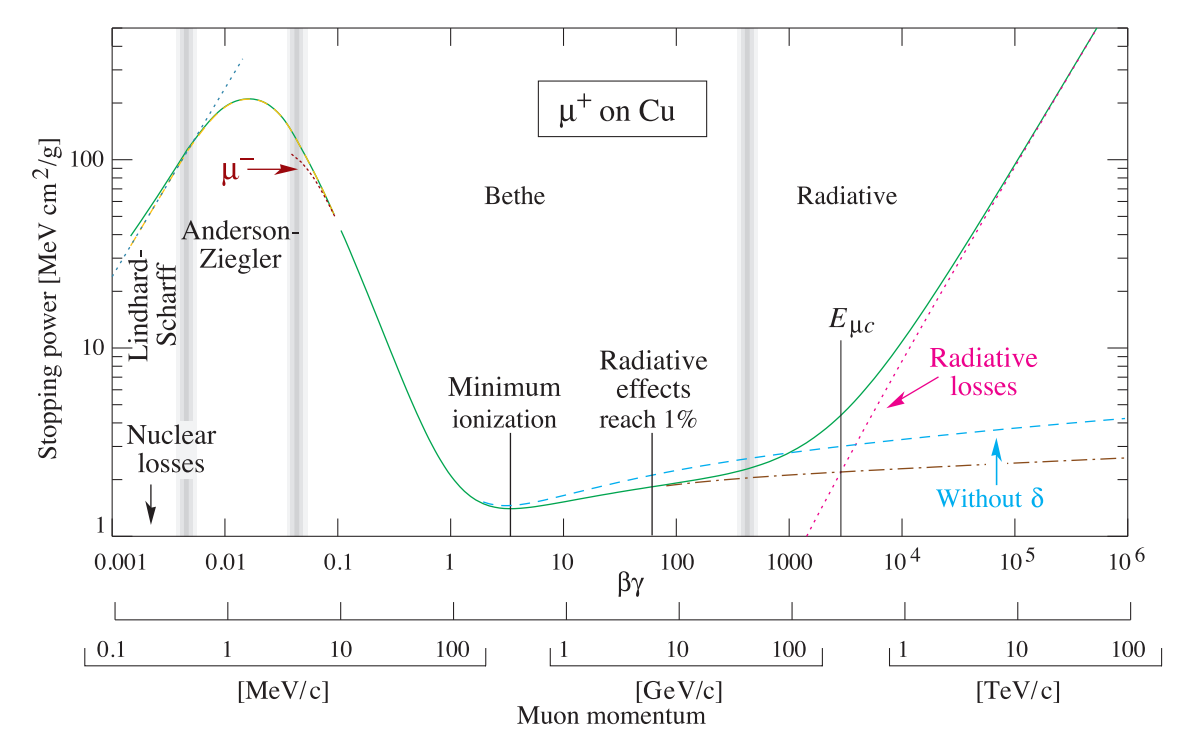
\includegraphics[width=.9\textwidth]{images/mu-pi-bethe.png}
  \caption{Energy loss by a muon in copper as a function of \( \beta\gamma \) or momentum. The solid line indicates the total stopping power, dashed lines indicate different contributions and the vertical grey bands indicate the different phenomenological regimes. Taken from ref~\cite{pdg}.}
  \label{fig:mu-pi-bethe}
\end{figure}
\begin{figure}[hptb]
  \centering  
    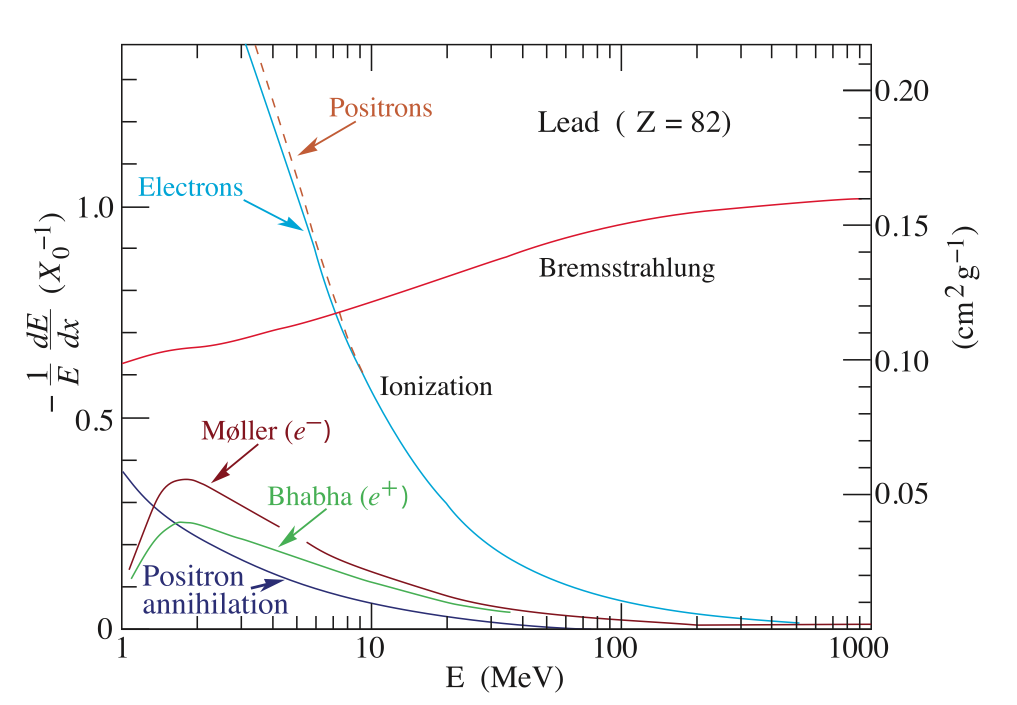
\includegraphics[width=.9\textwidth]{images/electron_energy_loss.png}
  \caption{Electron energy loss per `radiation length' (\( X_0^{-1} \)) as a function of electron energy (not momentum). The material in this case is lead (\(Z=82\) and \(X_0 = 6.37\)g/cm\(^2\)). Taken from ref~\cite{pdg}.}
  \label{fig:electron_energy_loss}
\end{figure}

At MuSIC the loss of energy by charged particles to matter is very important as it is the main method for detecting particles, and hence, characterising, the beam. When a particle deposits energy in a certain materials they will produce light, this light can then be detected giving information on the beam. The exact amount of light produced is dependent on the material and the amount of energy deposited but for many materials it can be approximated to a linear function of energy deposited. There are obviously problems with assuming linear light yields but a larger problem is the non-linear function for energy deposition. 

% section charged_particle_interactions_in_matter (end)
%%%%%%%%%%%%%%%%%%%%%%%%%%%%%%%%%%%%%%%%%%%%%%%%%
\subsection{Muon decay} % (fold)
\label{sec:muon_decay}
As has been noted muons decay \(\approx100\)\% of the time through the process: \( \mu \rightarrow e \nu \overline{\nu}  \). This process is the same for both positive and negative muons, although there is a sign change and the neutrino/anti-neutrino flavours will swap. The biggest difference between positive and negative muons is that negative muons can become bound to a nucleus in same way as electrons. This section will start with a general discussion of the important parameters of muon decay and then continue with a discussion of how this property of negative muons changes their decay.

The decay of a muon, like any other decay, can be modelled using the distribution:
\begin{equation}\label{eq:poisson}
  P(t) = Ne^{-t/\tau}
\end{equation}
Where \( P(t) \) is the survival probability of a particle after time, \( t \); \( N \) is a scaling factor to the size of the initial population and \( \tau \) is the population's lifetime. For a free muon in a vacuum the lifetime is \( \sim2.2\)~\( \mu \)s. As figure~\ref{fig:muon_decay_feynmann} shows the muon decay is mediated by a charged W boson, the presence of the two neutrinos mean that the only practically detectable result of the muon decay is the electron. The muon's (comparatively) long lifetime makes identification of them possible through by plotting decay times; this is discussed in greater detail in part~\ref{prt:characterising_the_beam}. 

\begin{figure}[hptb]
  \centering
    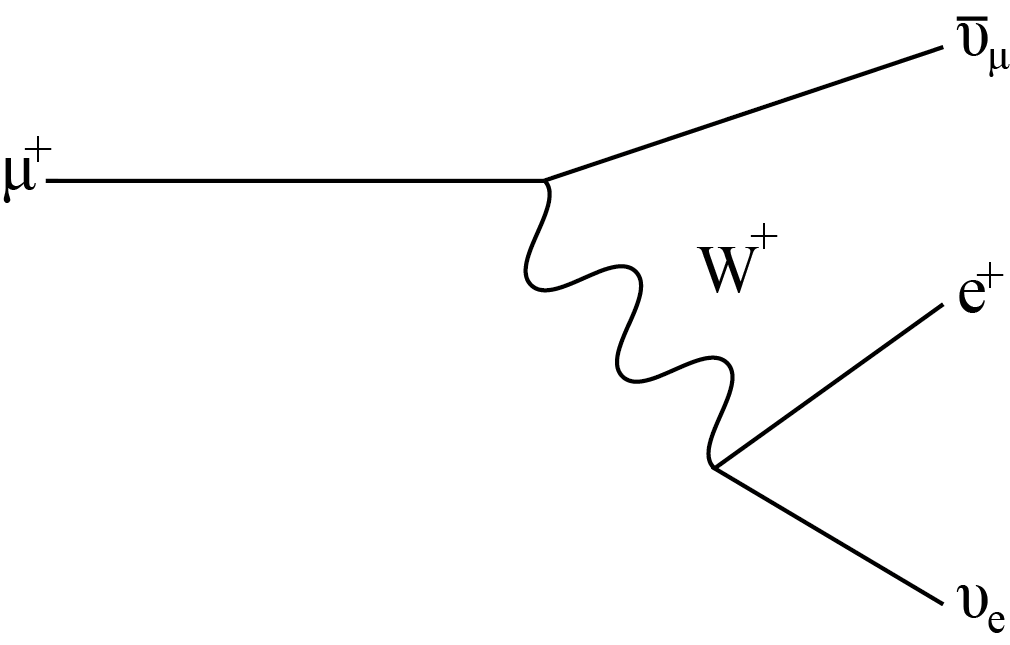
\includegraphics[scale=1]{images/muon_decay_feynmann.png}
  \caption{Feynman diagram showing muon decay.}
  \label{fig:muon_decay_feynmann}
\end{figure}

As has been noted negative muons can undergo an additional interaction with matter compared to positive muons. As a negatively charged lepton they can be become bound to a nucleus, reducing its lifetime as it loses energy falling through the nucleus' shells. The lifetime of a bound muon can be expressed as the reciprocal of an interaction rate:
\begin{align}
  \tau_{\mu^-} &= (\Delta_t)^{-1}\\
  \Delta_t &= \Delta_c + Q\Delta_d \label{eq:capture_rate}
\end{align}
where \( \Delta_t \) is the total interaction rate; \( \Delta_c \) is the rate of nuclear muon capture; \( \Delta_d \) is the rate of decay for positive muons (i.e.\ \( \tau_{\mu^+} = (\Delta_d)^{-1}  \)) modified by the `Huff-factor', \( Q \), which compensates for the reduction in energy available for a bound muon to decay. The positive, rather than negative, muon decay rate is used as the negative rate is less precisely known because of it's ability to bind to a nucleus.

When a negative muon is captured by a nucleus its lifetime is reduced compared to the positive muon. This reduction is due to the muon forming a muonic atom with its captor that allows it to rapidly shed energy via X-rays as it cascades through various shells until it enters the \( 1s \) state. The muonic cascade is a very rapid event, in most materials it occurs in less than \( 10^{-13}\)s~\cite{review_nuclear_physics_mu_capture_measday}, once in the \( 1s \) state the muon will decay much sooner having lost most of its energy. As will be discussed in parts~\ref{part:simulation}~and~\ref{part:measurement} these differing lifetimes give us some insight into the ratio of positive to negative muons.

A theoretical approximation to \( \Delta_c \) as a function of atomic mass, \( A \), and atomic number, \( Z \), was devised by Primakoff and Goulard~\cite{goulard_primakoff}:
\begin{align}
  \Delta_c(A,Z)&=Z^4_{eff} G_1 \left[ 1 + G_2 \frac{A}{2Z} - G_3 \frac{A-2Z}{2Z} - G_4 \left[\frac{A-Z}{2A} + \frac{A-2Z}{8AZ} \right] \right]
  \label{eq:primakoff_and_goulard}
\end{align}
Where the values \(G_{1-4}\) are parameters to be fitted and \( Z_{eff} \) is the effective value for the atomic number, as calculated by Ford and Wells~\cite{ford_and_wills_mesonic_atoms}, which accounts for the muon's \( 1s \) radius being much smaller than an electrons. The difference between the predicted capture rate and the measured rate is given in figure~\ref{fig:primakoff-goulard_vs_exp} with the fitted values of \(G\) shown in table~\ref{tab:g1_to_g4}. As can be seen there is still a fairly large disagreement between the theory and measured values for many atoms.

\begin{figure}[hptb]
  \centering
    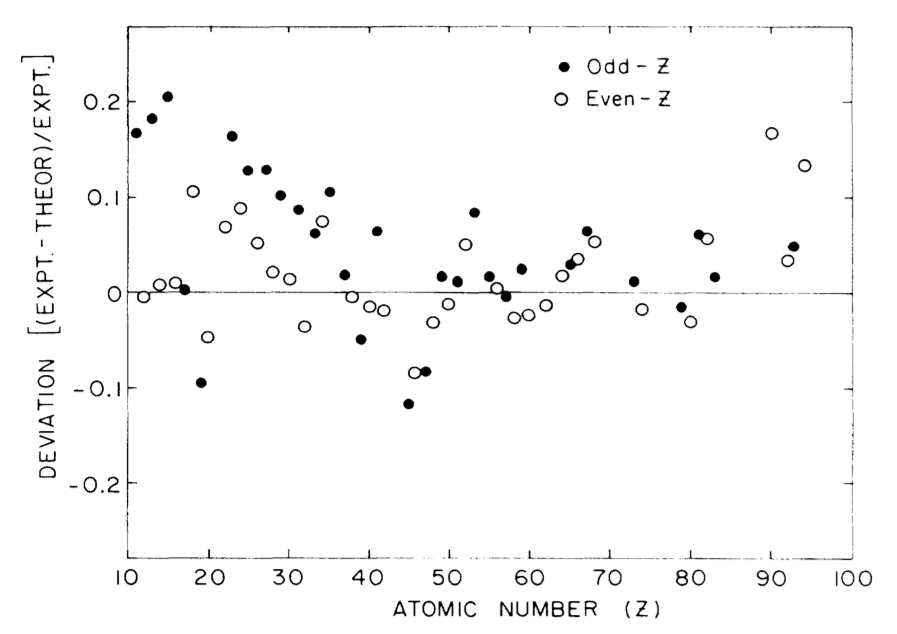
\includegraphics[width=.9\textwidth]{images/primakoff-goulard_vs_exp.png}
  \caption{Comparison of the theoretical values (as determined using the Primakoff-Goulard formula) and experimentally determined capture rates for a range of materials, taken from~\cite{suzuki_mu_capture_rates}.}
  \label{fig:primakoff-goulard_vs_exp}
\end{figure}

\begin{table}
  \begin{center}
  \begin{tabular}{c | r@{.}l | r@{.}l }
                                                              & \multicolumn{2}{c|}{TRIUMF data} & \multicolumn{2}{c}{Past Results}  \\
    \hline
    Number of data                                            & \multicolumn{2}{c|}{30}          & \multicolumn{2}{c}{58}            \\
    \hline
    \( G_1 \)                                                 &             260 &                &              252 &                \\
    \( G_2 \)                                                 &              -0 & 040            &               -0 & 038            \\
    \( G_3 \)                                                 &              -0 & 26             &               -0 & 24             \\
    \( G_4 \)                                                 &               3 & 24             &                3 & 23             \\
    \hline
    \( (\textrm{Expt.} - \textrm{Fit})/\textrm{Expt.} \) (\%) &               4 & 1              &                5 & 6              \\
  \end{tabular}
  \end{center}
  \caption{Experimentally determined values of \( G_1 \)--\( G_4 \) as determined by TRIUMF~\cite{suzuki_mu_capture_rates}.}
  \label{tab:g1_to_g4}
\end{table}


% section muon_decay (end)
%%%%%%%%%%%%%%%%%%%%%%%%%%%%%%%%%%%%%%%%%%%%%%%%%%%
\subsection{Charged Lepton Flavour Violation} % (fold)
\label{sec:charged_lepton_flavour_violation}
The discovery that neutrinos have mass and that they undergo flavour mixing shows that lepton flavour is not conserved, making charged Lepton Flavour Violation (cLFV) a possibility. 

Under the standard model of particle physics the simplest diagram of cLFV is when the emitted muon neutrino is virtual (see figure~\ref{fig:images_cLFV_mu-e_conversion}), for this to be true it must undergo conversion before being absorbed by the electron; the rate of this is governed by the neutrino mixing angles and, under the standard model, has a very small branching ratio~\cite{effective_lagrangian_for_clfv}. E.g.\ for \( \mu\rightarrow e\gamma \), the branching ratio is: 
\begin{align}
  \text{Br}(\mu\rightarrow e\gamma) 
    &= \frac{3\alpha}{32\pi}
      \left|\sum\limits_{i=2,3} U^*_{\mu i} U_{ei}
            \frac{\Delta m^2_{i1}}{M^2_W}
     \right|^2 \\
    &< 10^{-54} \label{equ:clfv_branching_ratio}
\end{align}
where \( U_{\nu i}^{(*)} \) are elements of the neutrino mixing matrix, \(\Delta m^2_{i1}\) is difference in neutrino masses and \(M_{W}\) is the mass of the W-boson.

This extremely low branching ratio makes cLFV it a `smoking gun' for new physics, should such a process be observed then it clearly indicates physics beyond the standard model. As a cLFV process has never been seen all current experiments have only been able to set upper limits on the branching ratio, the current world best is a limit of \(7\times10^{-13}\) set by SINDRUM~II in measuring \(\mu+Au\rightarrow e+Au\)~\cite{sindrum_2_mu_ag_e}.\footnote{This is an effective branching ratio in order to make direct comparisons with over cLFV processes easier.}

\begin{figure}[hptb]
  \centering
    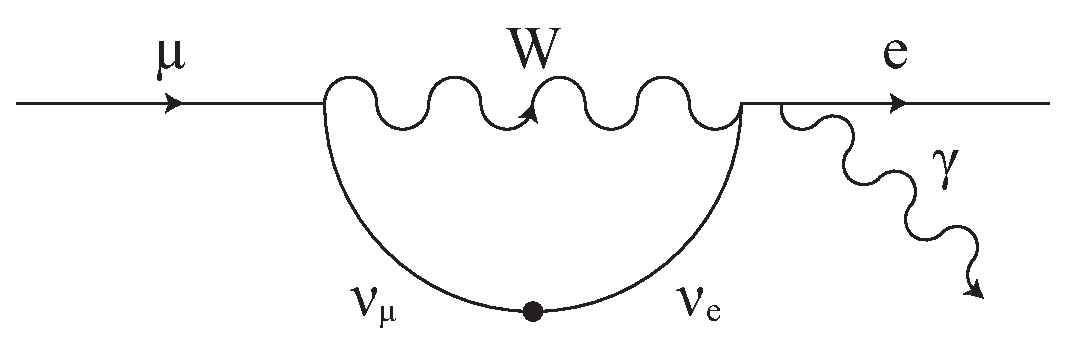
\includegraphics[width=.7\textwidth]{images/cLFV_mu-e_conversion.eps}
  \caption{\(\mu\rightarrow e\gamma\), as a standard model process. The black dot represents the conversion of the muon neutrino to an electron neutrino, in the standard model this process has a predicted branching ratio \(\sim <10^{-54} \) and has not been seen.}
  \label{fig:images_cLFV_mu-e_conversion}
\end{figure}

There are three core cLFV processes of interest: \( \mu\rightarrow e\gamma \), \( \mu\rightarrow eee \) and  \(\mu+X\rightarrow e+X \) (where \(X\) is an atomic nucleus), the current limits of these processes are given in table~\ref{tab:clfv}. At higher energies there are further processes involving taus (e.g.\ \(\tau\rightarrow\mu\gamma\)) and hadronic systems (e.g.\ \(K_L\rightarrow e\mu\)) but for brevity they will not be discussed here. 
\begin{table}
  \begin{center}
  \begin{tabular}{c | r@{\( \times \)}l | c}
    Process                  &  \multicolumn{2}{c|}{Limit}  &  Experiment \\
    \hline
    \(\mu\rightarrow e\gamma\)  &  \(<2.4\) & \(10^{-12}\)  &  MEG        \\
    \(\mu\rightarrow eee\)      &    \(<1\) & \(10^{-12}\)  &  SINDRUM    \\
    \(\mu+Au\rightarrow e+Au\)  &    \(<7\) & \(10^{-13}\)  &  SINDRUM II \\
    
  \end{tabular}
  \end{center}
  \caption{Current limits on the standard cLFV processes for muons. Note that several different materials have been tested for the process \( \mu + X\rightarrow e + X \) but the gold measurement, made at SINDRUM II, is currently the most accurate.}
  \label{tab:clfv}
\end{table}

Comparisons of the limits in table~\ref{tab:clfv} with the branching ratio under the standard model (equation~\eqref{equ:clfv_branching_ratio}) show there is still large regions of phase space that has yet to be excluded. Many beyond the standard model theories predict higher branching ratios for cLFV processes through the addition of loop diagrams; by placing limits on the rates of the these processes the mass scale of the model can be constrained. If cLFV is observed in multiple processes then it becomes possible to constrain the model further as the branching ratios for the different processes are linked via the Lagrangian that describes them.

To study the general features of a model that includes measurable cLFV an effective Lagrangian can be constructed, one such Lagrangian, taken from \cite{effective_lagrangian_for_clfv}, is:
\begin{align}
  \mathcal{L}_{cLFV} &= 
      \frac{m_{\mu}}{(\kappa + 1)\Lambda^2}
      \overline{\mu}_R\sigma_{\mu\nu}e_L F_{\mu\nu} + 
      \frac{\kappa}{(1+\kappa)\Lambda^2}
      \overline{\mu}_R\gamma_{\mu}e_L
      (\overline{e}\gamma^{\mu}e) \label{equ:type2}
\end{align}
where \(L\) and \(R\) are chirality; \(F^{\mu\nu}\) is the photon field strength and \( m_{\mu} \) is the muon mass. The operators are parameterised using two constants: \(\Lambda\), the effective mass scale, and \( \kappa \), a dimensionless parameter that determines the relative size of the Lagrangians' operators. In effect \(\kappa\) predicts the relative branching ratios between the different cLFV processes whilst \(\Lambda\) predicts at what mass new physics will occur. It's important to note that other effective Lagrangians exist but this is a good illustrative example. Figure~\ref{fig:images_clfv_type2} shows the relationship between \(\kappa\) and \(\Lambda\), as can be seen already excluded are mass scales up to 300~TeV. Should MuSIC improve on SINDRUM~I's limit for \( \mu\rightarrow eee \) by the predicted factor of 100 then the region up to 1,000~TeV will also be excluded. 

\begin{figure}[h]
  \centering
    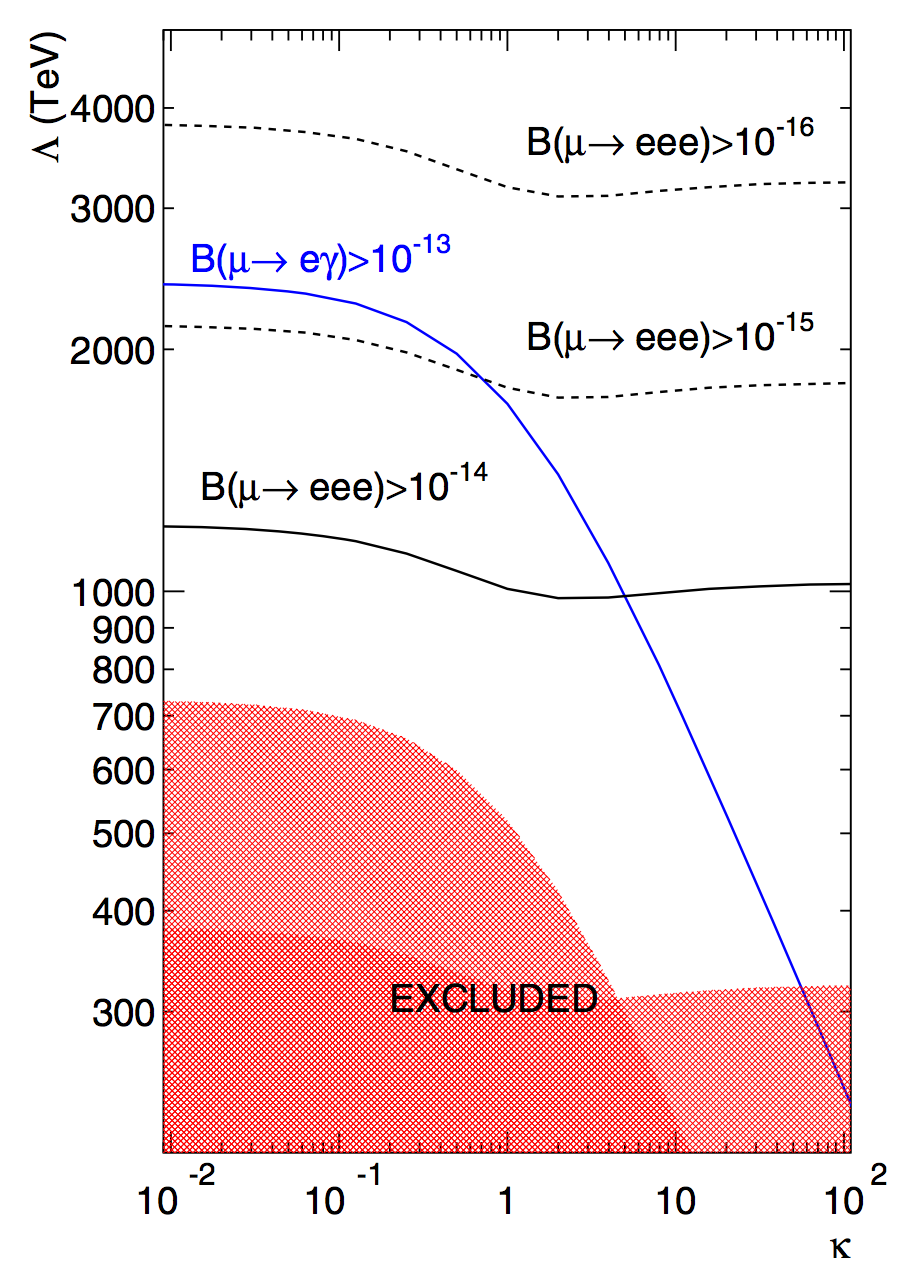
\includegraphics[width=.8\textwidth]{images/clfv_type2.png}
  \caption{Effective mass scale for expected sensitivities of \( \mu\rightarrow eee \) and \( \mu\rightarrow e\gamma \) experiments as a function of the scale parameter \( \kappa \), assuming a cLFV Lagrangian similar to equation~\eqref{equ:type2}. The target sensitivity for \( \mu\rightarrow eee \) measurements at MuSIC is shown in the solid black line.}
  \label{fig:images_clfv_type2}
\end{figure}

% section charged_lepton_flavour_violation (end)
% chapter physics (end)
%%%%%%%%%%%%%%%%%%%%%%%%%%%%%%%%%%%%%%%%%%%%%%%%%%%
% part introduction (end)
%%%%%%%%%%%%%%%%%%%%%%%%%%%%%%%%%%%%%%%%%%%%%%%%%%%
    \chapter{Simulation} % (fold)
\label{prt:simulation}
\section{Introduction} % (fold)
\label{cha:sim_introduction}
MuSIC was simulated to aid design of the detectors as well as to improve analysis of the data produced. Two core simulations were created, one using G4Beamline (G4BL) and the other using Geant4. 

The G4BL simulation was mainly used to simulate the bulk of MuSIC and the hadron interactions. A more detailed and configurable Geant4 simulation was used to simulate the detectors. This section will discuss the general features of Geant4 and G4BL before a more detailed discussion of the actual implementation. The discussion will focus on the work done on the Geant4 simulation for the fifth MuSIC beam time as this was the most complete simulation performed. Simulations were used in earlier beam times but not to the same extent, although the G4BL simulation was used to interpret the total charged particle flux measurements. Less simulation work was done for the muon lifetime measurement as it was simpler to compare the measured lifetimes with precise values made by other experiments.

\section{Geant4} % (fold)
\label{sec:geant4}
Geant4 is described as `a toolkit for the simulation of the passage of particles through matter'~\cite{geant4}. Rather than a complete program it is a collection of pre-compiled libraries that comprise the basics required to simulate various interactions. It has additional libraries that provide further functionality such as visualisation. 

Geant4 is written in C++ using an object orientated approach that allows the user to either use Geant4's implementation of a class or write their own. This flexibility also means that all the functionality of Geant4 is explicitly opt-in, making the resultant programs much faster than they would otherwise be (as only the components that are selected are used). Geant4's speed does come at a cost which is that a larger amount of configuration is required than would be needed for less flexible solutions (e.g.\ G4BL).

Even with its increased flexibility Geant4 has certain requirements that must be met in order to work. These requirements embody the minimum information needed for Geant4 to create a simulation. The requirements are a definition of what to simulate, where to simulate it and the processes to simulate. Geant4's base requirement is that there is an instance of one of each of three classes\footnote{Whilst there is a technical distinction between an instance of a class (an object) and the class itself for the sake of clarity the word `class' is used throughout.}:
\begin{description}
  \item[The detector constructor] -- a description of the space in which the particle is to be simulated.
  \item[The physics list] -- which physical processes to simulate.
  \item[The primary action generator] -- a description of the initial particle to simulate.
\end{description}
With these three classes defined a simple program can be linked with the Geant4 libraries and run. The libraries use the primary action generator to create the initial particle, its interactions are described by the physics list and the world is specified by the detector constructor. In addition to these required components a simulation can be further refined with custom classes that replace or expand those supplied by Geant4.

The rest of this section will discuss how Geant4 uses the above three classes, and several others, to simulate a particle. This discussion will be split into two: discussion of the detector constructor and discussion of Geant4's execution model. The detector constructor will be treated separately as it is a primarily static description of a space. The execution model will cover the dynamic aspects of the simulation, e.g.\ how physical processes are implemented.

% subsection material_simulation (end)
\subsection{Detector Constructor} % (fold)
\label{sub:detector_constructor}
The detector constructor has two key jobs: defining the materials and defining the volumes of the detector. The materials describe the physical properties of various elements, compounds and mixtures. The volumes describe the position, rotation, material and logical attributes of the detector. 

\subsubsection{Material Properties} % (fold)
\label{ssub:material_properties}

The material properties in Geant4 can be thought of as members of one of two sets: referred to here as `core' and `extended'. The core properties cover those values that are required for reasonable calculations of energy loss in the material, the extended properties cover more detailed calculations and properties that are more specialised.

The core properties for an element are the atomic number, the mass number and the molar density. Compounds and mixtures are described as ratios of their component elements at a specific density. Extended properties can be any property of the material that the user is interested in, for our purposes these were the optical properties of the materials and are discussed below.

Due to the computationally complex nature of interactions between light and material Geant4 doesn't implement them by default. When enabled Geant4 uses single values or tables of values to describe the various optical processes that it can simulate. The tables it uses are defined in terms of photon energy and missing values are generated via interpolation. 
% subsubsection material_properties (end)

\subsubsection{Detector Volumes} % (fold)
\label{ssub:detector_volumes}

The detector volumes describe the physical pieces of the detector. Each volume to be simulated has its description split between three classes: the geometry, the logical volume and the physical volume. The geometry describes the shape and size of the volume. The logical volume describes how the volume relates to the larger simulation. Finally the physical volume places and orientates the volume with respect to the other volumes.

The volume's geometry is normally described by either basic polyhedra (cubes, tubes, trapezoids etc.) or compound shapes made from basic polyhedra. Geant4 provides basic tools for creating compounds made of the intersection, difference and addition of other geometries (either basic polyhedra or other compound polyhedra). Using these tools it's possible to create suitably complex constructions in code. Geant4 does offer more powerful tools (e.g.\ geometry importing) but these were not used for this simulation.

The logical volume stores the specific attributes of the component. The main information that the logical volume maintains is what material a component is (this can be changed using messengers) and what shape it is. A single logical volume can be associated with many physical volumes to make repetitive constructs easy to define.

As has been noted the physical volume positions the component. Additionally it stores which logical volume this component is in (as well as which logical volume describes it). Storing the parent volume means that a single logical volume can contain many sub-components to make bulk manipulation easier, as all placements are done with respect to the parent volume's origin.

% subsubsection detector_volumes (end)
\subsection{Execution model} % (fold)
\label{sub:execution_model}

Geant4 manages simulation by splitting it into several layers with each layer representing a level of complexity within the simulation. The top-most level is the \emph{run}, this represents a collection of \emph{events} and all the information that is static between them (e.g.\ the detector configuration). An event is a collection of particle \emph{tracks}. Each event starts with an initial particle (as defined by the primary action generator) the particle's track is split into \emph{steps} with each step representing a period of time in which nothing `significant' happens. As significant processes occur (e.g.\ particle decay) new tracks (to represent the new particles) are added to the event and they too stepped through their simulation. A track finishes when either the particle decays (and produces new tracks), it leaves the simulated volume or comes to rest. Once all the tracks finish, the event is over and the next event begins. Normally the user will specify the number of events that any run should contain, although other criteria can be used (e.g.\ a time out).
% whose subsequent interactions are then simulated, if another particle is produced (e.g.\ if the initial particle decays) then a new track is added to the event to represent the new particle(s). 
% A track is made up of \emph{steps}, each step represents a period of time in which nothing `significant' occurs.

A `significant' occurrence is one which will make further calculations of properties of the particle difficult and therefore limit the length of the particle's step. Determination of this step length is split between multiple classes within Geant4 but they can be broadly separated into four categories: detector considerations, user imposed limits, continuous physical processes and discrete physical processes. In each category the method is broadly the same, any class that can have an affect on the particle calculates a distance from the current position at which the affect will occur, e.g.\ a detector may report that the particle will leave the current volume in 10~mm whilst a decay process may report that the particle will likely decay in 5~mm. Once all the proposed step lengths have been determined the shortest is found and the particle is transported that distance and properties (position, time, energy, particle type(s)\footnote{Should the particle decay it is replaced at the end of the step with the appropriate daughter particles.} etc.) are updated. 

As has been stated the main consideration for the step length with respect to the detector are the volume boundaries which generally delimitate a change in material that will obviously determine which processes occur and how. Other detector considerations include the affect of a field on the particle's transport. Continuous processes generally only limit a particle by reducing its energy to zero (obviously some processes can increase it but these rarely limit a step length). Discrete processes obviously limit a particle by changing it in some way, for example by having a particle decay. Once a step length has been determined any continuous affects are applied to the particle, if it's at a volume boundary it moves into the next volume, any limiting discrete processes are applied and the next step length is calculated. 

The processes (discrete or continuous) are supplied by the physics list. The physics list registers which processes can occur to which particles and then assigns a class to handle that eventuality. In this way physical processes can be enabled or disabled at will. It is also possible to register several classes to a single particle-process pair in order to describe different situations the most common use of this is to apply different models depending on particle energy. Obviously the full range of physical processes that need to be described to accurately simulate the Standard Model is quiet large, luckily Geant4 has extensive pre-compiled lists that cover the major types of particle interaction as well as several specialised lists that cover specific situations e.g.\ low energy regimes which are often ignored in high energy simulations as they can be computationally expensive. 

% subsection execution_model (end)
% section geant4 (end)
%%%%%%%%%%%%%%%%%%%%%%%%%%%%%%%%%%%%%%%%%%%%%%%%%%%
\section{G4beamline} % (fold)
\label{sec:g4beamline}
G4beamline (G4BL) is a program written by Muons, Inc.~\cite{g4bl}; it is a particle tracking simulation program that uses Geant4. Unlike Geant4, G4BL is a pre-compiled program where the user writes simple scripts that define the parameters of the simulation. In general creating simulations in G4BL is much quicker than Geant4 as a significant amount of `boilerplate' code is removed at the cost of flexibility. The use of Geant4, rather than G4BL, for the detector simulation was mainly driven by the finer control Geant4 offered.

G4BL simulates the major interactions that a particle can undergo but cannot simulate optical processes, detectors and has more limited output options than Geant4. The physics used in G4BL is less well optimised for low energy than Geant4 can be made to be. It also does not have the same flexibility as Geant4 does for use with macros.

% section g4beamline (end)
%%%%%%%%%%%%%%%%%%%%%%%%%%%%%%%%%%%%%%%%%%%%%%%%%%%
% chapter sim_introduction (end)
\section{Implementation} % (fold)
\label{cha:implementation}
As has been discussed the simulation was split between G4BL and Geant4. This section will focus on the implementation of the Geant4 detector simulation as this constituted the bulk of the work carried out.

\subsection{G4Beamline} % (fold)
\label{sec:g4beamline_impl}
G4BL was used to describe the bulk of MuSIC: the initial proton beam, the pion capture solenoid: target, capture solenoid, the shielding and return yoke; and the transport solenoids: bending magnets and pipe sections. A virtual detector, with radius 50~cm, was placed at the end of the beam pipe and recorded the particles that pass through it. A wireframe rendering of the set up can be seen in figure~\ref{fig:images_Geometry_g4bl_wireframe} the co-ordinates used for the simulation and analysis are defined on it: \(X\) is horizontal across the beam pipe, \(Y\) is vertical across the beam pipe and \(Z\) is in the direction of the beam.

\begin{figure}[hptb]
  \centering
    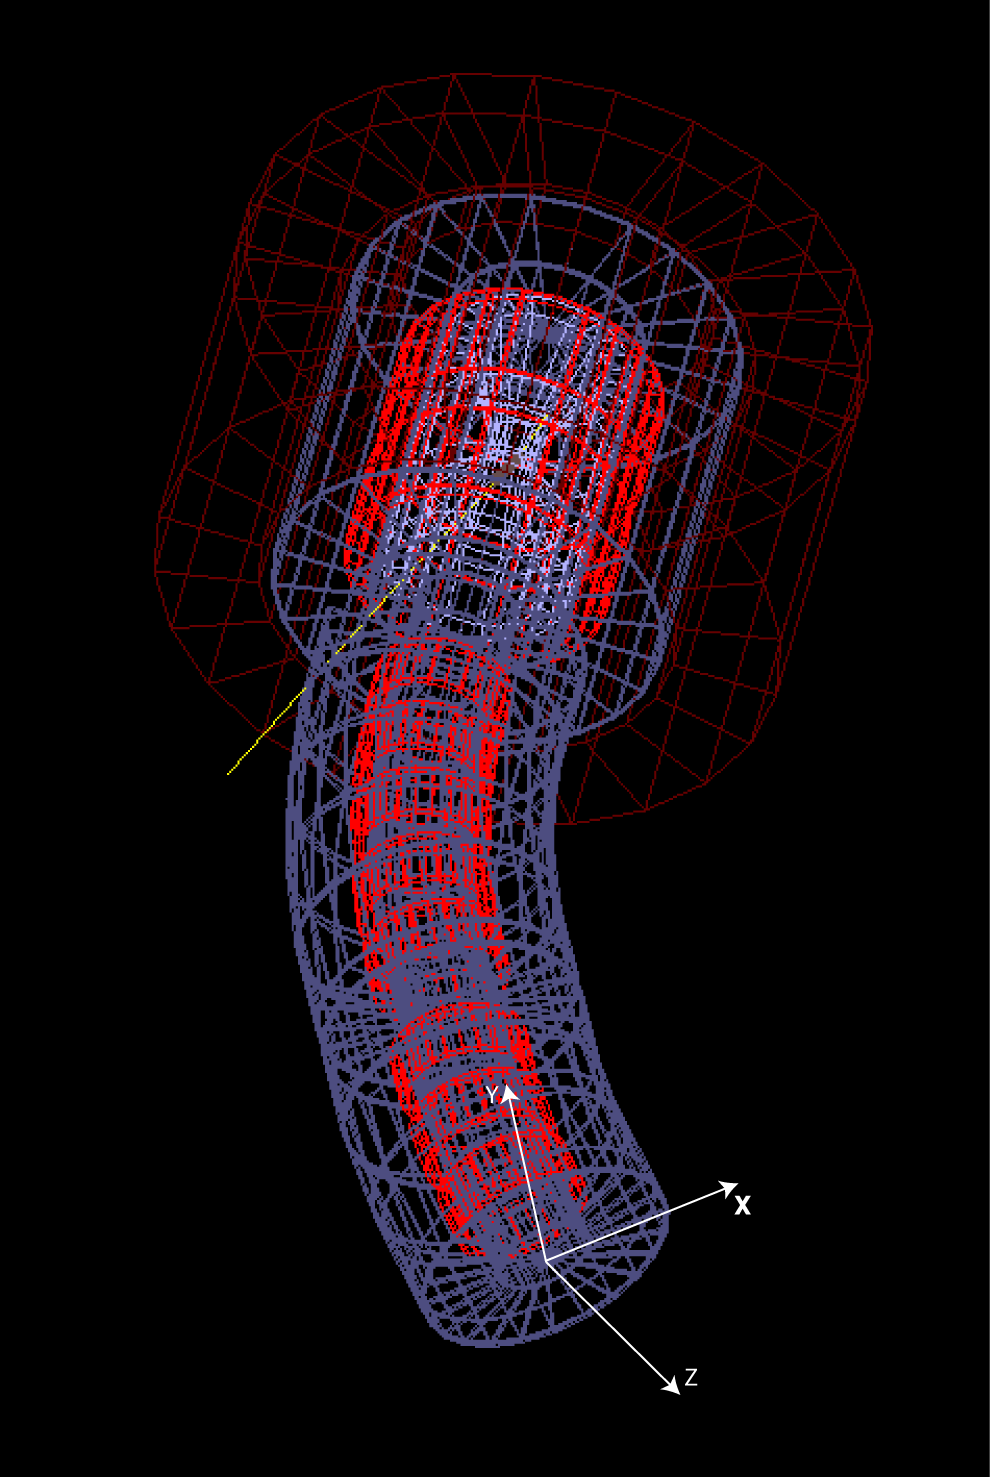
\includegraphics[width=.75\textwidth]{images/Geometry/g4bl_wireframe.png}
  \caption{Wireframe of the G4BL simulation of MuSIC. The dark red is the iron yoke, the bright red are the solenoids, the light blue is the pion capture solenoid shielding and the yellow line is a simulated proton which doesn't interact in this case. The co-ordinates used are defined at the end of the beam pipe.}
  \label{fig:images_Geometry_g4bl_wireframe}
\end{figure}

Using this script G4BL, simulated the computationally expensive hadronic interactions at the production target. The output of the G4BL simulation could then be reused for multiple detector set ups by importing the particle distribution into Geant4.

G4BL was used to simulate 900~million initial protons, the resulting beam at the end of the MTS was used as input for the Geant4 simulation. Figure~\ref{fig:images_sim_2d_per_pid_flux} shows the flux for each particle type whilst figure~\ref{fig:images_sim_2d_charged_particle_flux} shows the total charged particle distribution at the end of the beam-pipe. Table~\ref{tab:g4bl_particle_counts} shows the number of each particle type and the mean position. As figure~\ref{fig:images_sim_2d_per_pid_flux} shows the positive and negative particles split with this most clearly seen in the heavier pions and muons. Obviously the total particle flux is dominated by the electrons with the muons spread across the beam.


The evolution of the final distribution is shown in figure~\ref{fig:images_pid_counts_in_beamline} with the position of the monitors used shown in figure~\ref{fig:images_g4bl_monitor_locations_bigger_edit}. The conversion of positive pions into positive muons can be seen with the increase of the latter at the second position.

\begin{table}[hptb]
  \begin{center}
  \begin{tabular}{c | r | r@{\(\pm\)}l | r@{\(\pm\)}l | r@{\(\pm\)}l | r@{\(\pm\)}l}
    \multicolumn{1}{c|}{\multirow{2}{*}{Particle}} 
               &   \multicolumn{1}{c|}{\multirow{2}{*}{Count}} 
                             &  \multicolumn{4}{c|}{Horizonal position (mm)}
                                              &  \multicolumn{4}{c}{Vertical position (mm)}    \\
               &             &  \multicolumn{2}{c|}{Mean}  
                                                   &  \multicolumn{2}{c|}{RMS}  
                                                         &  \multicolumn{2}{c|}{Mean}  
                                                                    &  \multicolumn{2}{c|}{RMS}  \\
    \hline
      e\(^-\)  &  1,362,161  &  \(-\)61.55 & 0.05  &  62.29 & 0.04  &       98.73 & 0.04  &  44.62 & 0.03  \\
      e\(^+\)  &    183,074  &  \(-\)37.10 & 0.16  &  67.91 & 0.11  &       50.20 & 0.15  &  66.03 & 0.11  \\
    \(\mu^-\)  &      8,940  &  \(-\)45.10 & 0.75  &  70.97 & 0.53  &       65.35 & 0.69  &  65.54 & 0.49  \\
    \(\mu^+\)  &     86,480  &  \(-\)26.12 & 0.27  &  79.55 & 0.19  &   \(-\)1.75 & 0.27  &  79.16 & 0.19  \\
    \(\pi^-\)  &      4,169  &  \(-\)57.50 & 0.99  &  63.99 & 0.70  &       84.65 & 0.87  &  56.27 & 0.62  \\
    \(\pi^+\)  &     53,406  &  \(-\)44.19 & 0.32  &  72.79 & 0.22  &  \(-\)28.50 & 0.32  &  74.04 & 0.23  \\
       p       &     60,589  &  \(-\)43.37 & 0.30  &  73.15 & 0.21  &  \(-\)26.28 & 0.31  &  76.80 & 0.22  \\
    \(\overline{\text{p}}\)
               &          0  & \multicolumn{2}{c|}{n/a}  
                                                   &  \multicolumn{2}{c}{n/a}
                                                                    & \multicolumn{2}{c}{n/a}
                                                                               &  \multicolumn{2}{c}{n/a}  \\
       n       &     88,553  &   \(-\)8.31 & 0.33  &  98.84 & 0.23  &        0.10 & 0.31  &  92.78 & 0.22  \\
  \end{tabular}
  \end{center}
  \caption{Summary of the particle distributions at the end of the MuSIC beam-pipe for 900~million initial protons. The number of particles of that type are given along with the mean and RMS of their distribution along the horizontal and vertical axis.}
  \label{tab:g4bl_particle_counts}
\end{table}

\begin{sidewaysfigure}[hptb]
  \centering
    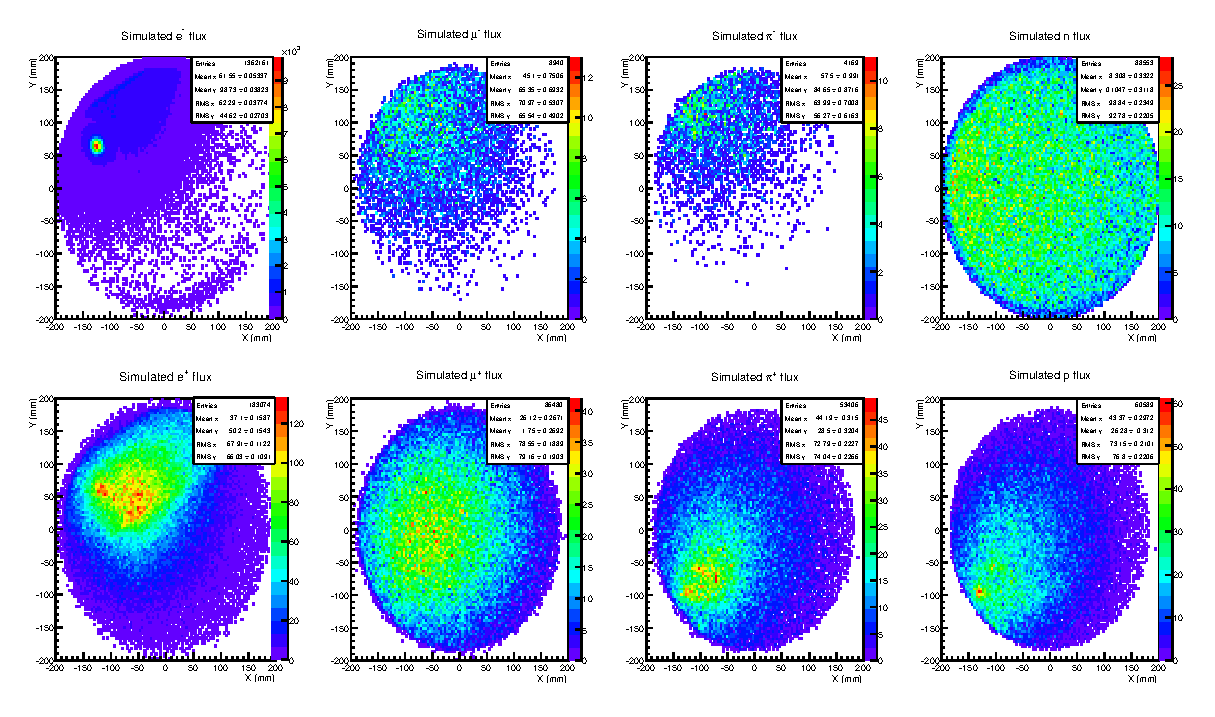
\includegraphics[width=.9\textwidth]{images/sim_2d_per_pid_flux.eps}
  \caption{Distributions of the different charged particles in co-ordinates \(X\) against \(Y\) at the end of the MuSIC beam-pipe.}
  \label{fig:images_sim_2d_per_pid_flux}
\end{sidewaysfigure}

\begin{figure}[hptb]
  \centering
  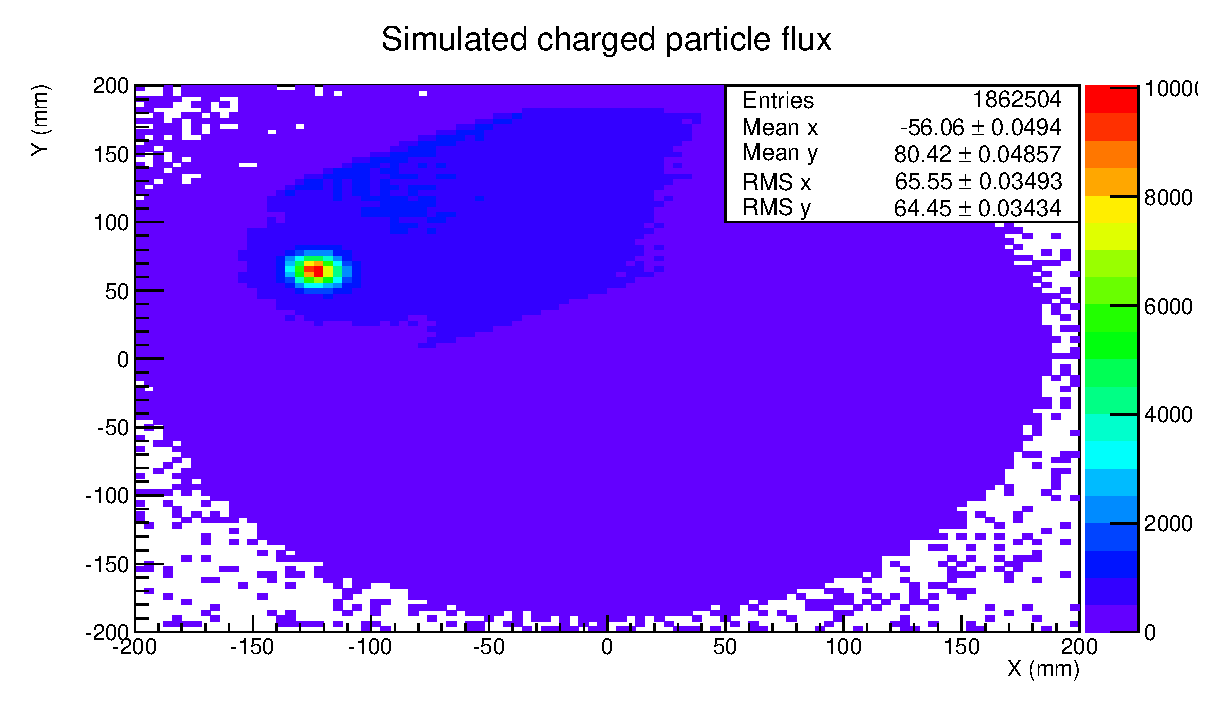
\includegraphics[width=.9\textwidth]{images/sim_2d_charged_particle_flux.eps}
  \caption{Distribution of total charged particle flux for \(X\) against \(Y\) at the end of the MuSIC beam-pipe.}
  \label{fig:images_sim_2d_charged_particle_flux}
\end{figure}


\begin{figure}[hptb]
  \centering
    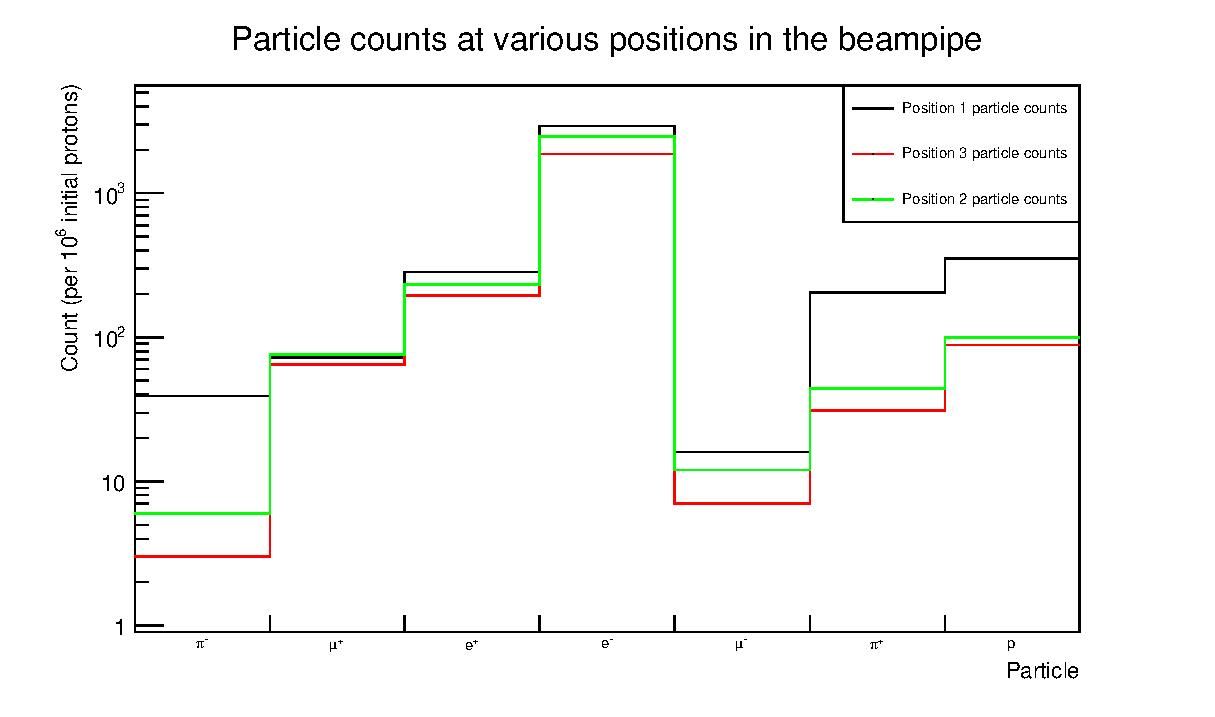
\includegraphics[width=.9\textwidth]{images/pid_counts_in_beamline.eps}
  \caption{Evolution of the particle distribution in the G4BL simulation of MuSIC. Position 1 is 1~cm after the pion capture solenoid and positions 2 and 3 are after the first dipole and at the end of the beam pipe respectively.}
  \label{fig:images_pid_counts_in_beamline}
\end{figure}

\begin{figure}[hptb]
  \centering
    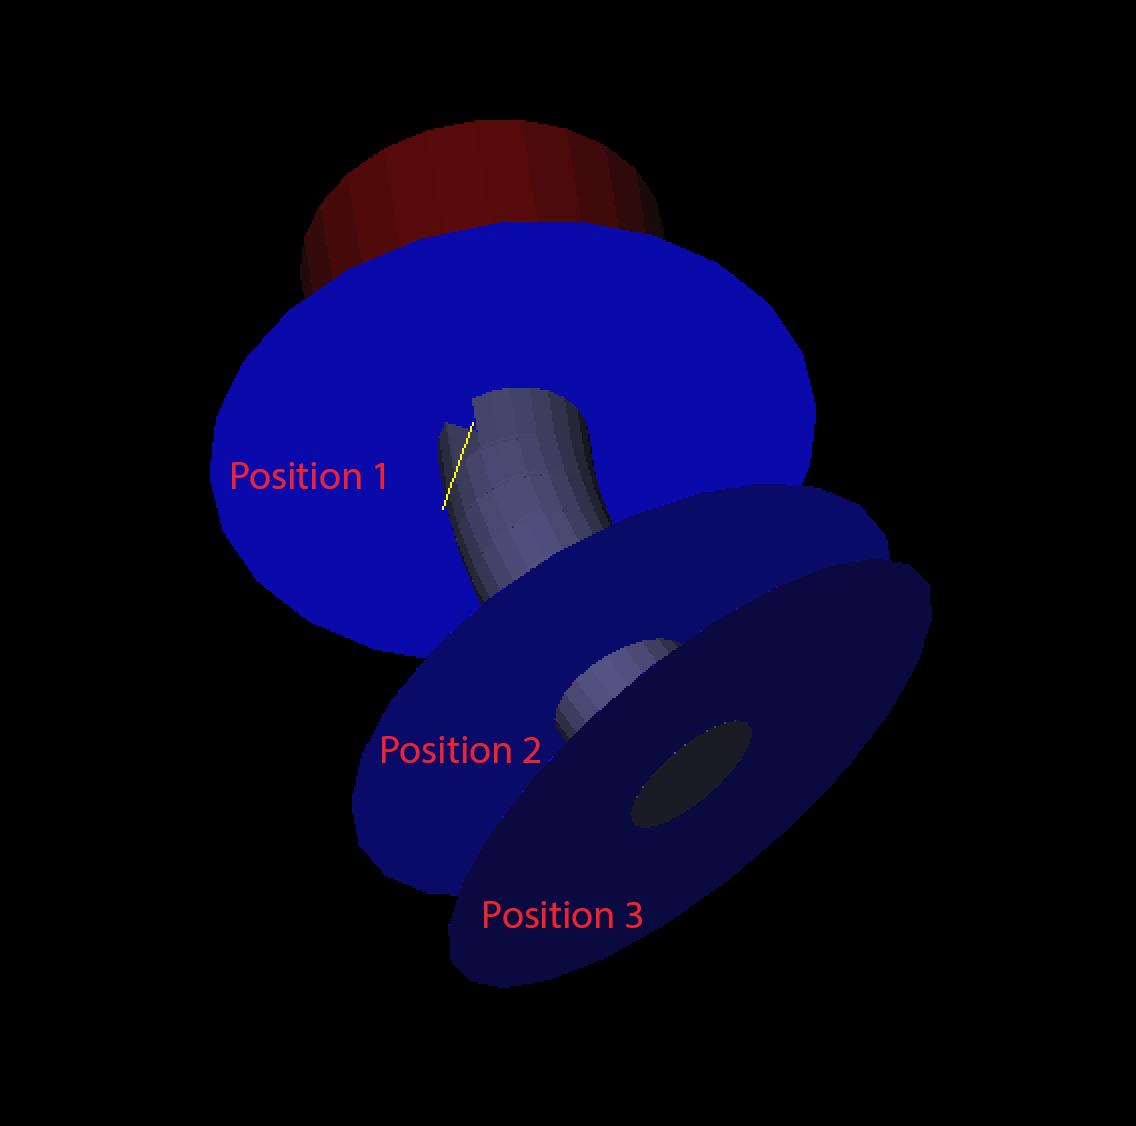
\includegraphics[width=.9\textwidth]{images/g4bl_monitor_locations_bigger_edit.png}
  \caption{Position of the beam monitors used to track the particle distribution through the G4BL simulation. Note: the monitors used to create the distribution used in the final Geant4 simulation have a much smaller, 50~cm, radius compared to 2~m used in this image (as the smaller radius monitors would not be visible).}
  \label{fig:images_g4bl_monitor_locations_bigger_edit}
\end{figure}
\clearpage
% section g4beamline (end)
\subsection{Geant4} % (fold)
\label{sub:geant4}
The Geant4 simulation was split into several key classes in addition to the detector constructor, primary action generator and physics list previously discussed. These classes were:
\begin{description}
  \item[The magnetic field] which gave the field strength within the detector.
  \item[The stepping action] which analysed every step of a particle's track and if it passed certain criteria, passed the track to ROOT for recording.
  \item[ROOT] which read and wrote ROOT files that were used to import the G4BL distribution and record events from the stepping action.
  \item[The messengers] a set of classes for configuring the simulation without re-compiling the program.
\end{description}
The implementation of each of these classes will now be discussed with the exception of the ROOT and messenger classes which primarily implemented utilities and had no impact upon the simulation or the data it produced.

The messengers were used to specify parameters to be used in the following run. These parameters are supplied via configuration files called macros. Four aspects of the simulation were controlled via macros: the primary action generator, the physics list, the magnetic field and the detector constructor. It was then possible to write further scripts that generated macros to test a range of configurations, e.g.\ a script was used to generate several macros that ran the simulation with a range of different detector setups.

% subsection geant4 (end)
\subsection{Detector Constructor} % (fold)
\label{sec:detector_constructor}
The detector constructor is by far the most complex of the classes used in the simulation. The implementation of the detector construction was split over several functions, this discussion will follow similar lines. The materials will be discussed, then the optical properties and finally the geometry of the detector. Prior to these more detailed discussions a more holistic view of the detector will be given.

The detector simulated is the same as that used in the final measurements of the muon momentum spectrum. A schematic of the detector is shown in figure~\ref{fig:images_Detector_setup_music5}. The detector has four core components: the degrader, two counters and a stopping target. The layout of the components is: degrader; thin, upstream counter; stopping target; then finally the thicker downstream counter. The degrader and stopping target of plates of pure metal (aluminium and copper respectively). The counters are each composed of several strips of scintillator (8 in the upstream counter and 5 in the downstream). Each scintillator strip has a Wave-Length Shifting (WLS) fibre mounted on the back of it which (in the experiment) was connected to a Multi-Pixel Photon Counter (MPPC). A schematic of a strip can be seen in figure~\ref{fig:images_counter_schematic}.

\begin{figure}[hptb]
  \centering
    \includegraphics[width=.9\textwidth]{images/Detector_setup_music5.png}
  \caption{Schematic of the detector configuration for simulation.}
  \label{fig:images_Detector_setup_music5}
\end{figure}

\begin{figure}[hptb]
  \centering
    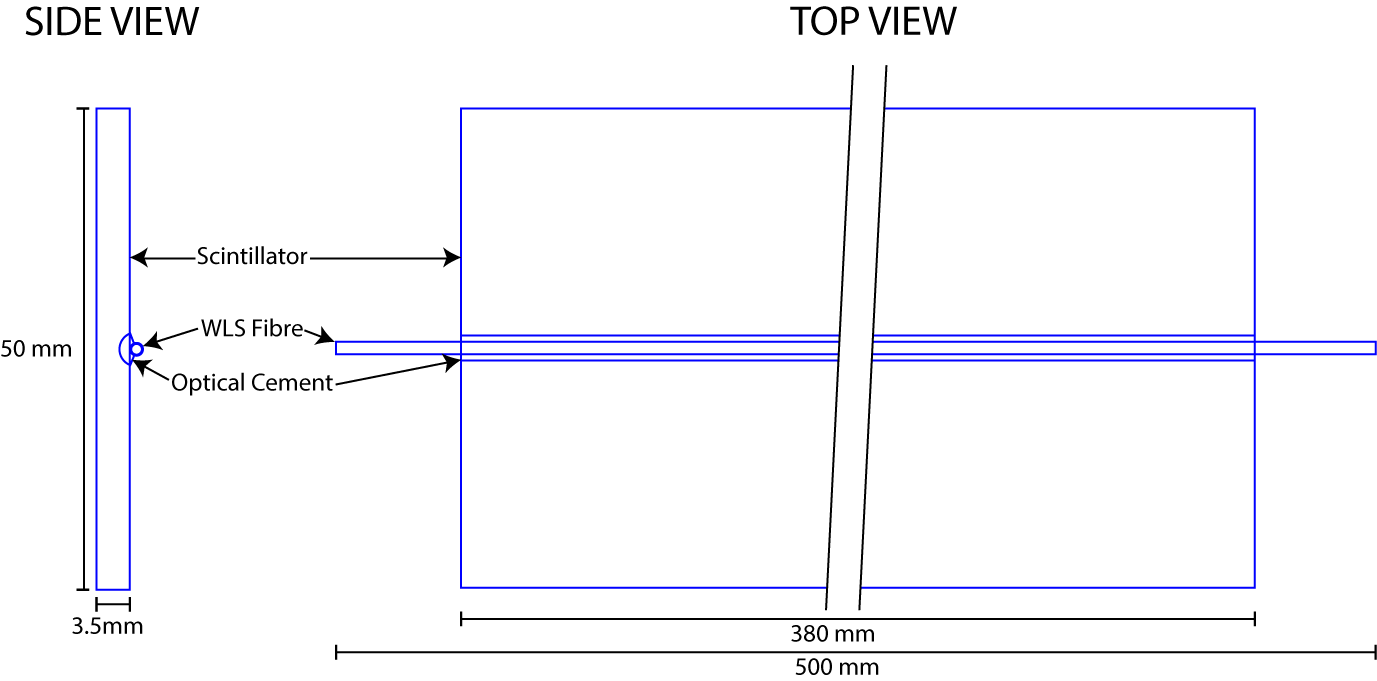
\includegraphics[width=.9\textwidth]{images/counter_schematic.png}
  \caption{Schematic of a downstream paddle. The upstream paddles have the same layout but are have a different width and height (0.5~mm and 30~mm respectively). The WLS fibre protrudes from the scintillator for easy attachment of the MPPCs to the support structure.}
  \label{fig:images_counter_schematic}
\end{figure}


\subsubsection{Materials} % (fold)
\label{ssub:implementation_materials}

To simulate the detectors at MuSIC a fairly simple selection of materials were required, the elemental metals used for the stopping target and degrader; and several plastics that made up the scintillators. Geant4 treats materials as either pure elements or as mixtures (even if they're a compound). For the materials used at MuSIC only six elements were needed (H, C, N, O, Al and Cu), these had their standard values for mass number, atomic number and, where needed, density. The majority of these were used as components of plastics and for approximating the composition of air but copper and aluminium were used in their pure form (hence the inclusion of their density). 

The compounds and mixtures (table~\ref{tab:sim_compounds_and_mixtures}) were, with the exception of air, components of the scintillators. Mylar was used to wrap the scintillators; EJ-212~\cite{ej_212} (a trade name for NE-102A, based on polyvinyltoluene) is the core scintillating material; and BCF-91A~\cite{bcf_91a} is the (WLS) fibre, which has a polystyrene core with a PMMA cladding. The optical properties that were included in the simulation were:
\begin{enumerate}
  \item The refractive index, n.
  \item The emission spectrum that described the scintillation light produced by ionising particles.
  \item Absorption spectrum, used in concert with an additional emission spectrum this described the WLS fibres.
  \item Scintillation yield, for EJ-212 this was 10,000~MeV\(^{-1}\) as stated by the manufacturer and assumes a linear response.
\end{enumerate}
These properties were only implemented for the materials involved in the optical system. The emission and absorption spectra for the scintillator and WLS fibres were approximated to the curves given in the material data sheets (\cite{ej_212} and \cite{bcf_91a}), the values used are plotted in figures~\ref{fig:images_ej-212-g4}~and~\ref{fig:images_bcf-91a-g4} respectively.

\begin{table}
  \begin{center}
  \begin{tabular}{c | c | c | d{4} | c | c}
    Compound/  &  \multirow{2}{*}{Components}  
                               &  \multirow{2}{*}{Ratio}
                                             &  \multicolumn{1}{c|}{Density}
                                                       & Refractive
                                                                &  \multirow{2}{*}{Ref}  \\
    Element    &               &             &  \multicolumn{1}{c|}{(g/cm\(^3\))}
                                                       &  Index 
                                                                &        \\
    \hline
    Air        &     N, O      &     4 : 1     &  1.290  &  1.00  & --        \\
    Mylar      &   H, C, O     &   4 : 5 : 2   &  1.40   &   --   & \cite{groom2001_mylar_ref} \\
    EJ-212     &     H, C      &  5.17 : 4.69  &  1.023  &  1.58  & \cite{ej_212}      \\
    BCF-91A (core)  &  H, C    &  4.82 : 4.85  &  1.05   &  1.60  & \cite{bcf_91a}    \\
    BCF-91A (clad)  & H, C, O  &   8 : 5 : 2   &  1.2    &  1.49  & \cite{bcf_91a}    \\
    
  \end{tabular}
  \end{center}
  \caption{Compounds and mixtures used for the simulation. No refractive index is given for mylar as it's opaque. An additional property of EJ-212 was the light yield which was 10,000~MeV\(^{-1}\).}
  \label{tab:sim_compounds_and_mixtures}
\end{table}

\begin{figure}[hptb]
  \centering
    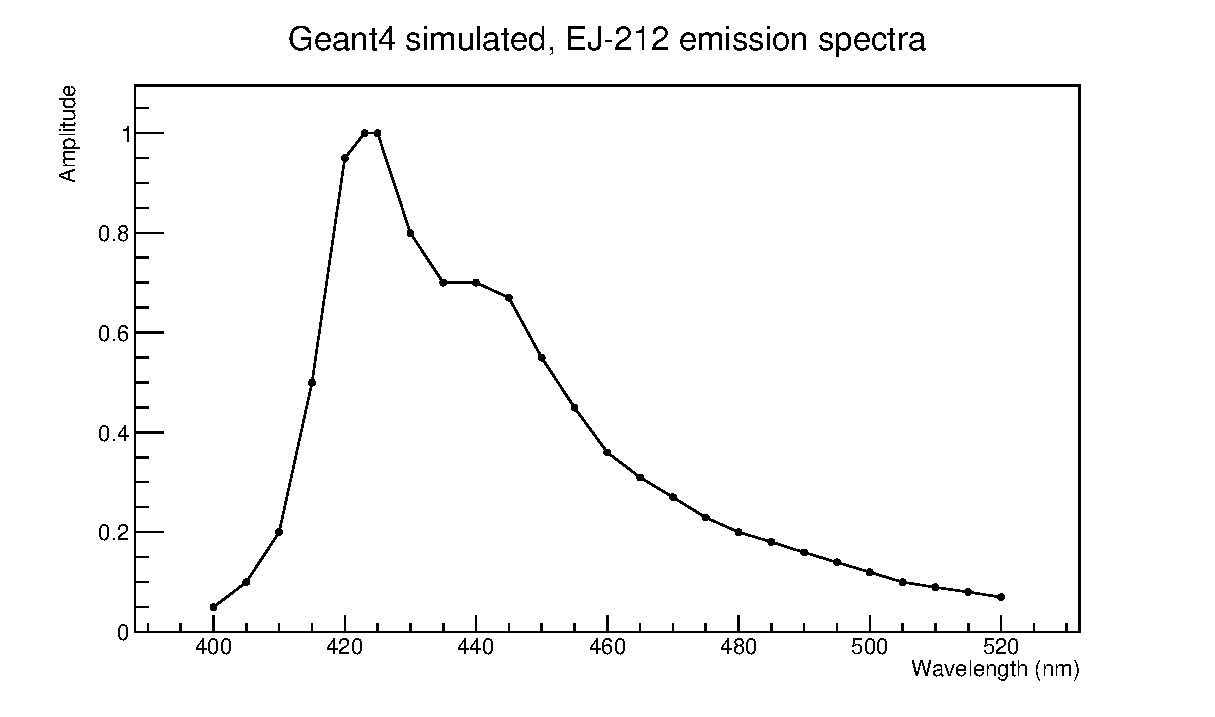
\includegraphics[width=.9\textwidth]{images/ej-212-g4.eps}
  \caption{Scintillation spectra for EJ-212. The points represent the values passed to Geant4 and are based on those read from the manufacturer's data-sheet~\cite{ej_212}.}
  \label{fig:images_ej-212-g4}
\end{figure}


\begin{figure}[hptb]
  \centering
    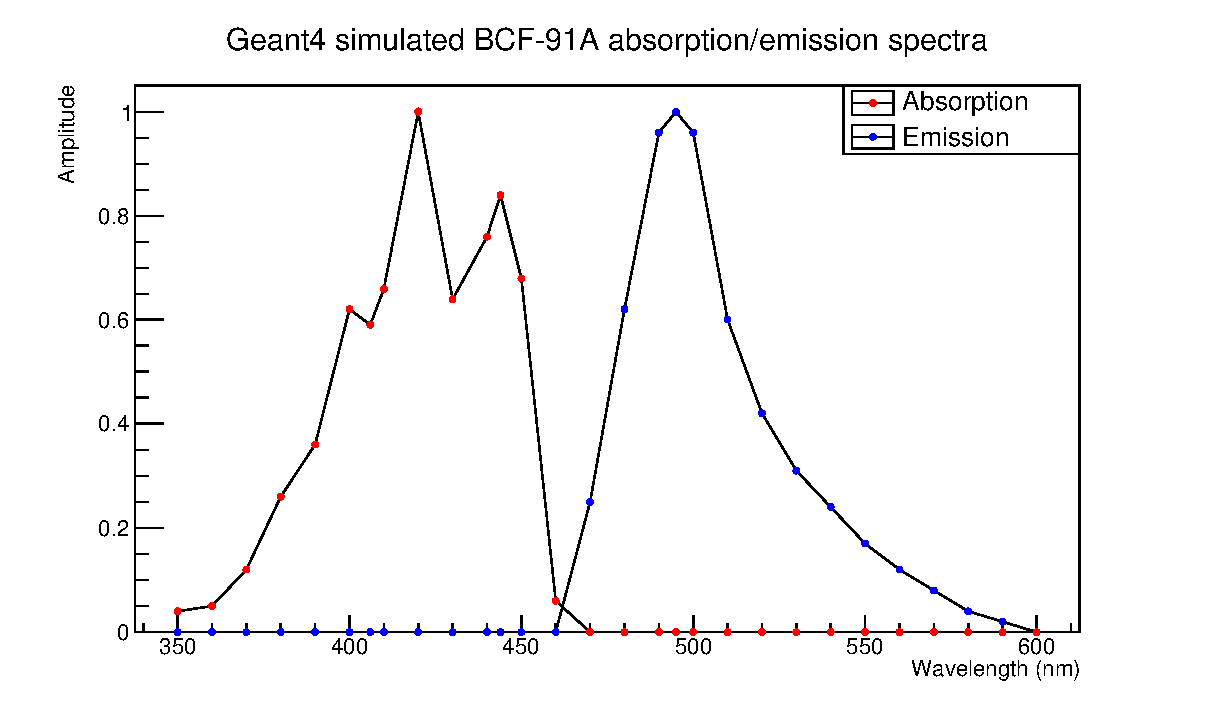
\includegraphics[width=.9\textwidth]{images/bcf-91a-g4.eps}
  \caption{Absorption and re-emission spectra for BCF-91A wavelength shifting fibre. The points represent the values used in Geant4 to approximate the manufacturer's curve as given in the data-sheet~\cite{bcf_91a}.}
  \label{fig:images_bcf-91a-g4}
\end{figure}

% subsubsection implementation_materials (end)
\subsubsection{Detector geometry} % (fold)
\label{ssub:implementation_detector_geometry}

MuSIC was simulated as an \(8\times8\times8\)~m\(^3\) volume of air containing the detector. The size of the volume was chosen to simplify transformations of the detector with respect to the magnetic field. The detector was implemented as four placed volumes inside a single logical volume that allowed all of them to be correctly positioned with respect to the magnetic field. The four sub-volumes were the upstream counter, the downstream counter, the degrader and the stopping target. This was the set-up used for the muon lifetime measurements and the final momentum spectrum measurements made during runs 4 and 5.

The degrader and stopping target were configured so that their material and thickness could be changed using macros. This made testing configurations prior to beam-time much quicker and easier. This also meant that the degrader could be removed by creating a volume of air. The materials used for the degrader and stopping target were simple elemental metals (aluminium and copper respectively). Both components were implemented as simple sheets with the dimensions given in table~\ref{tab:st_and_deg_dimensions}.

\begin{table}
  \begin{center}
  \begin{tabular}{c | c | c | c | c}
    \multirow{2}{*}{Component}
                     &  \multirow{2}{*}{Material} 
                                   &  \multicolumn{3}{c}{Dimension (mm)}  \\
                     &             &   X   &   Y   &       Z       \\
    \hline
    Stopping Target  &  Copper     &  370  &  310  &      0.5      \\
    Degrader         &  Aluminium  &  400  &  400  & 0, 0.5, 1, 5  \\
    
  \end{tabular}
  \end{center}
  \caption{Dimensions of the stopping target and degraders. The degrader width of 0~mm is when the degrader is removed and replaced with air. The \(Z\)~axis is the main beam direction with the \(X\) and \(Y\) axes being in the horizontal and vertical directions respectively.}
  \label{tab:st_and_deg_dimensions}
\end{table}

The counters were more complex. Each counter was split into a number of `strips' (eight upstream, five downstream). A strip was composed of a scintillator, a 135\(^{\circ}\) section of pipe (also made of scintillator material) that mimicked the optical cement and a length of wavelength shifting fibre (made of a core and shell). Mylar was then used to define an optical surface that existed at the boundary between scintillator and air. An optical surface is a special construct in Geant4 that is not a full volume but a set of physical effects that occur when optical photons move from one volume to the next, in this way the reflective effect of mylar wrapping was created. A \(1\times1\times1\)~mm\(^3\) volume of air is placed at the end of each wavelength shifting fibre to act as a Multi-Pixel Photon Counter (MPPC) detector region. A side on view of the layout of a paddle can be seen in figure~\ref{fig:images_Geometry_full_strip}, the dimensions used for the paddles are are given in table~\ref{tab:dimensions_of_paddles} the entire layout can be seen in figure~\ref{fig:images_Detector_setup_music5}.

\begin{table}
  \begin{center}
  \begin{tabular}{c | c | c | c}
    Component      & Material         & Number     &  Dimensions (mm\(^3\)) \\
    \hline
    Upstream              &  EJ-212          &  8         &  \(380\times30\times0.5 \) \\
    Downstream            &  EJ-212          &  5         &  \(380\times50\times3.5 \) \\
    WLS fibre (core)      &  BCF-91A (core)  &  1/paddle  &  
                                        \multirow{2}{*}{\(500\times(r=0.5)\)} \\
    WLS fibre (cladding)  &  BCF-91A (clad)  &  1/paddle  &  \\
    MPPC                  &  Air             &  2/paddle  &  \(1\times1\times1 \) \\
  \end{tabular}
  \end{center}
  \caption{Dimensions of the simulated paddle components. The wavelength shifting fibres were the same for both up- and down-stream counters, as were the `MPPCs'. The WLS fibre's cladding is said to be 3\% of the total diameter so this is what is used~\cite{bcf_91a}.}
  \label{tab:dimensions_of_paddles}
\end{table}

% section detector_constructor (end)
\subsection{Primary Action Generator} % (fold)
\label{sec:primary_action_generator}
The primary action generator is a relatively simple class that specifies the properties of the initial particle to be simulated. This means, for all implementations, defining the particle's type, position within the volume and initial momentum. 

At MuSIC the key task of the primary action generator was to either import the particle distribution from the G4BL simulation or create particles with a similar distribution. The source and type of particle could be configured using messengers.

% To import from G4BL the particle type, momentum and position were all read from the root file which G4BL saved them in. Approximations to G4BL were used for basic tests, the approximations were simple Gaussian (and double Gaussian) fits to the G4BL data. It was hoped that the approximations would yield results close enough to the G4BL simulation to be usable for comparison to data. It was found that the approximated distributions gave significantly different rates for stopping muons in the detector when compared to the G4BL distribution. This difference meant the approximations were only used to confirm the efficacy of the integration technique used to estimate the number of muons rather than for more detail comparisons which would have been desirable given the low number of negative muons in the G4BL sample. 

% section primary_action_generator (end)
\subsection{Physics List} % (fold)
\label{sec:physics_list}
Geant4 provides the majority of physics processes as precompiled lists that cover the major aspects of a simulation. For MuSIC the key attribute of each list was the accuracy at low energies. In this respect the most important lists were those dealing with electromagnetic processes. To cover this `option3' and the `extra' lists were used which have improved low energy simulations and more detailed processes. Most importantly the `extra' list implements muon capture at rest. The few hadronic processes were simulated with the `HP' QGSP-BERT and the elastic physics models, both of which have better methods for simulating low energy neutrons.

One problem with the default supplied physics lists is that the implementation of muon capture at rest is based mainly on theoretical work that doesn't accurately model the capture rate of muons on copper. This is obviously a problem as copper is the main stopping target used at MuSIC. The lifetime for muonic copper produced using unmodified Geant4 is \(\sim1.1\)~\(\mu\)s compared to the experimental value of 163.5~ns~\cite{suzuki_mu_capture_rates} or the theoretical value of 194~ns (calculated using equation~\cite{eq:primakoff_and_goulard}). This difference can be seen in  figure~\ref{fig:images_mu-_lifetime_in_cu_unmodded_g4} and figure~\ref{fig:images_mu-_lifetime_in_cu_modded_g4} which show the muon decay spectra of negative muons with the modified and un-modified versions of Geant4 respectively.

The modification used was to the `G4StopElementSelector' class where the function `GetMuonCaptureRate' had an additional element added to its precompiled lists of capture rates to correspond to the capture rate for muons in copper, which is \(5.72\pm0.05\times10^6\)~s\(^{-1}\). This was acknowledged as a bug by the Geant4 development team and has been fixed in more recent versions of the framework (i.e. more later than \( 4.9.6 \)~patch~02).

\begin{figure}[hptb]
  \centering
    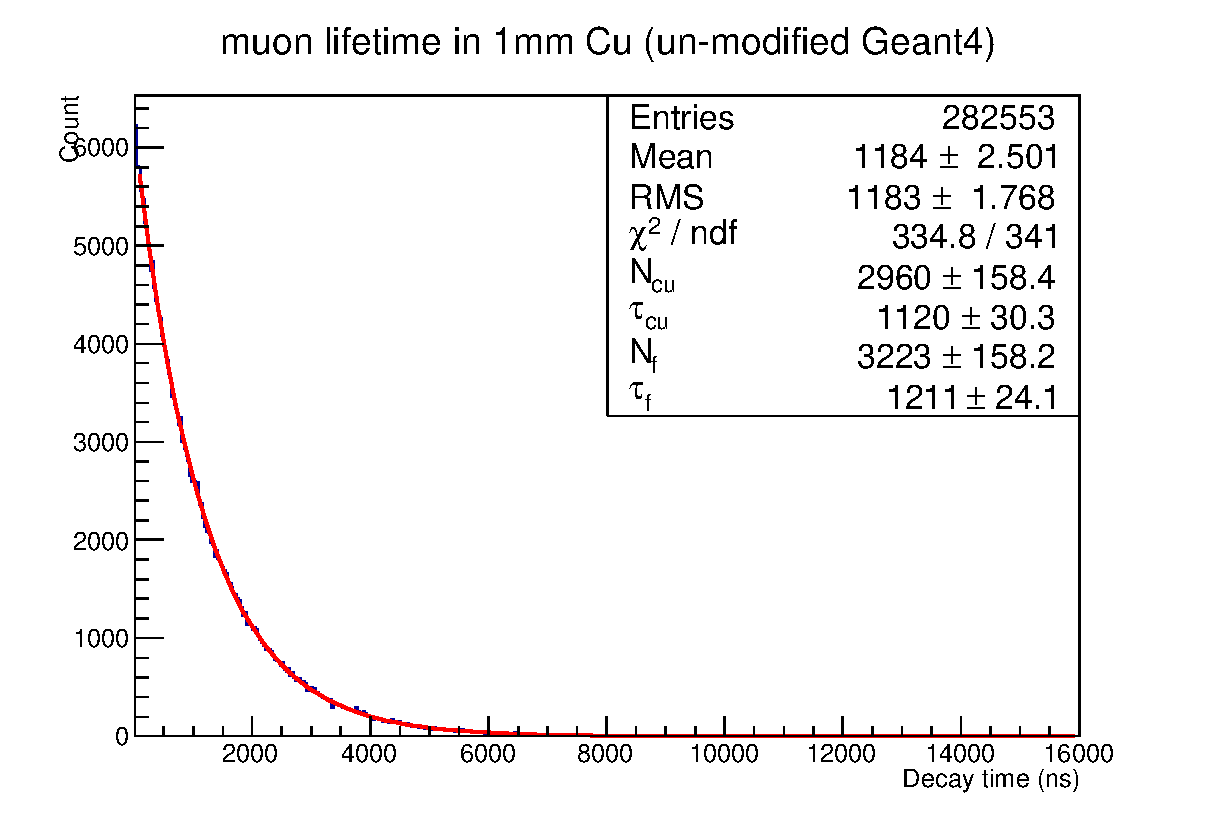
\includegraphics[width=.7\textwidth]{images/mu-_lifetime_in_cu_unmodded_g4.eps}
  \caption{Decay spectrum of \(1\times10^6\) negative muons hitting a 1~mm copper stopping target using an unmodified version of Geant4. The decay times are fitted using \(N\exp(-x/\tau)\). As can be seen the Geant4 value, 1,161~ns, does not agree with either the experimentally determined value of 163.5~ns~\cite{suzuki_mu_capture_rates} or the theoretical value of 194~ns (calculated using the equation~\ref{eq:primakoff_and_goulard}. This bug has been fixed in more recent versions of Geant4 (versions \(>\)~\( 4.9.6 \)~patch~02).}
  \label{fig:images_mu-_lifetime_in_cu_unmodded_g4}
\end{figure}

\begin{figure}[hptb]
  \centering
    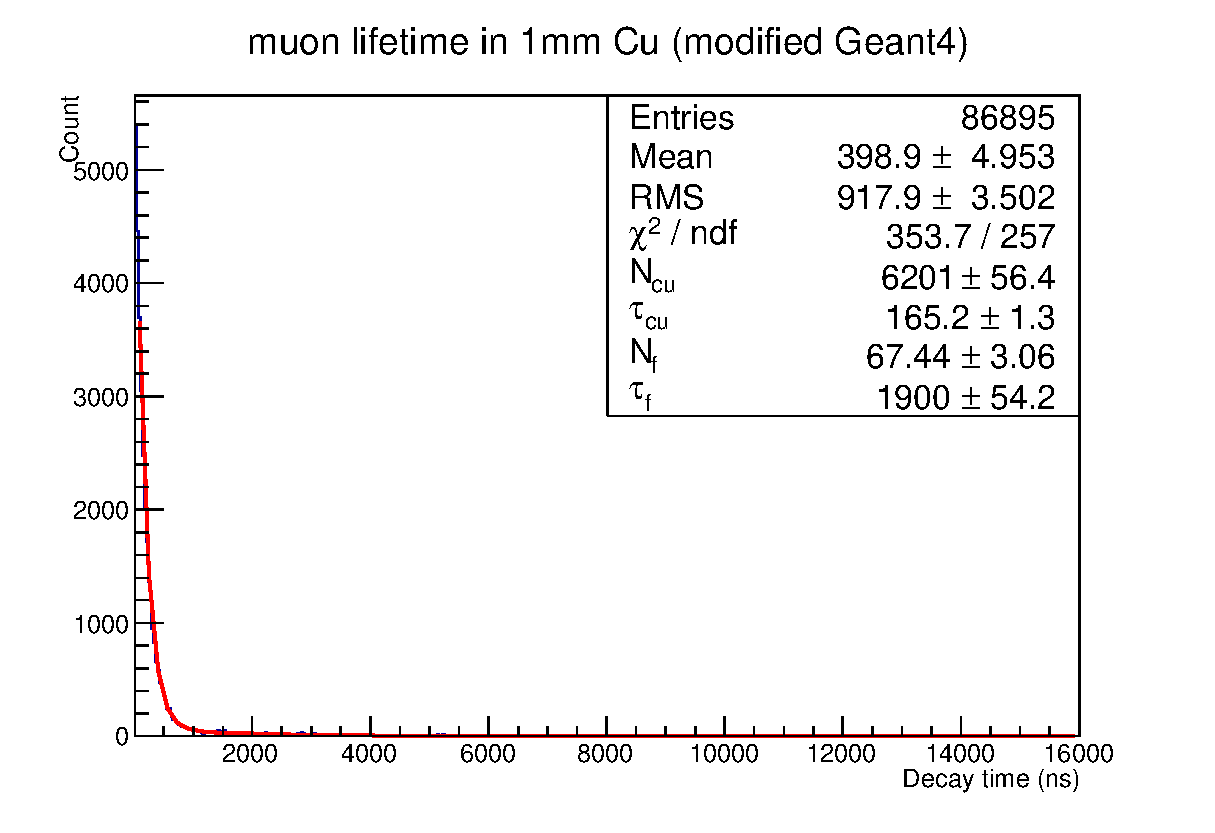
\includegraphics[width=.7\textwidth]{images/mu-_lifetime_in_cu_modded_g4.eps}
  \caption{Decay spectrum of \(1\times10^6\) negative muons hitting a 1~mm copper stopping target using a version of Geant4 modified to use the experimental muonic copper lifetime of 163.5~ns. The spectrum is fitted using \(N\exp(-x/\tau)\).}
  \label{fig:images_mu-_lifetime_in_cu_modded_g4}
\end{figure}


% section physics_list (end)
\subsection{The Field} % (fold)
\label{sec:the_field}
Field maps for the entire detector region were available but to improve efficiency only the region directly surrounding the detector was simulated, this is shown in figure~\ref{fig:images_field_map_edited}. Geant4 uses interpolation to find values for the magnetic field that weren't present in the file. The file listed position and the magnetic field at each position. To save space the file relied on the vertical symmetry to account for the lower half of the detector.

\begin{figure}[hptb]
  \centering
    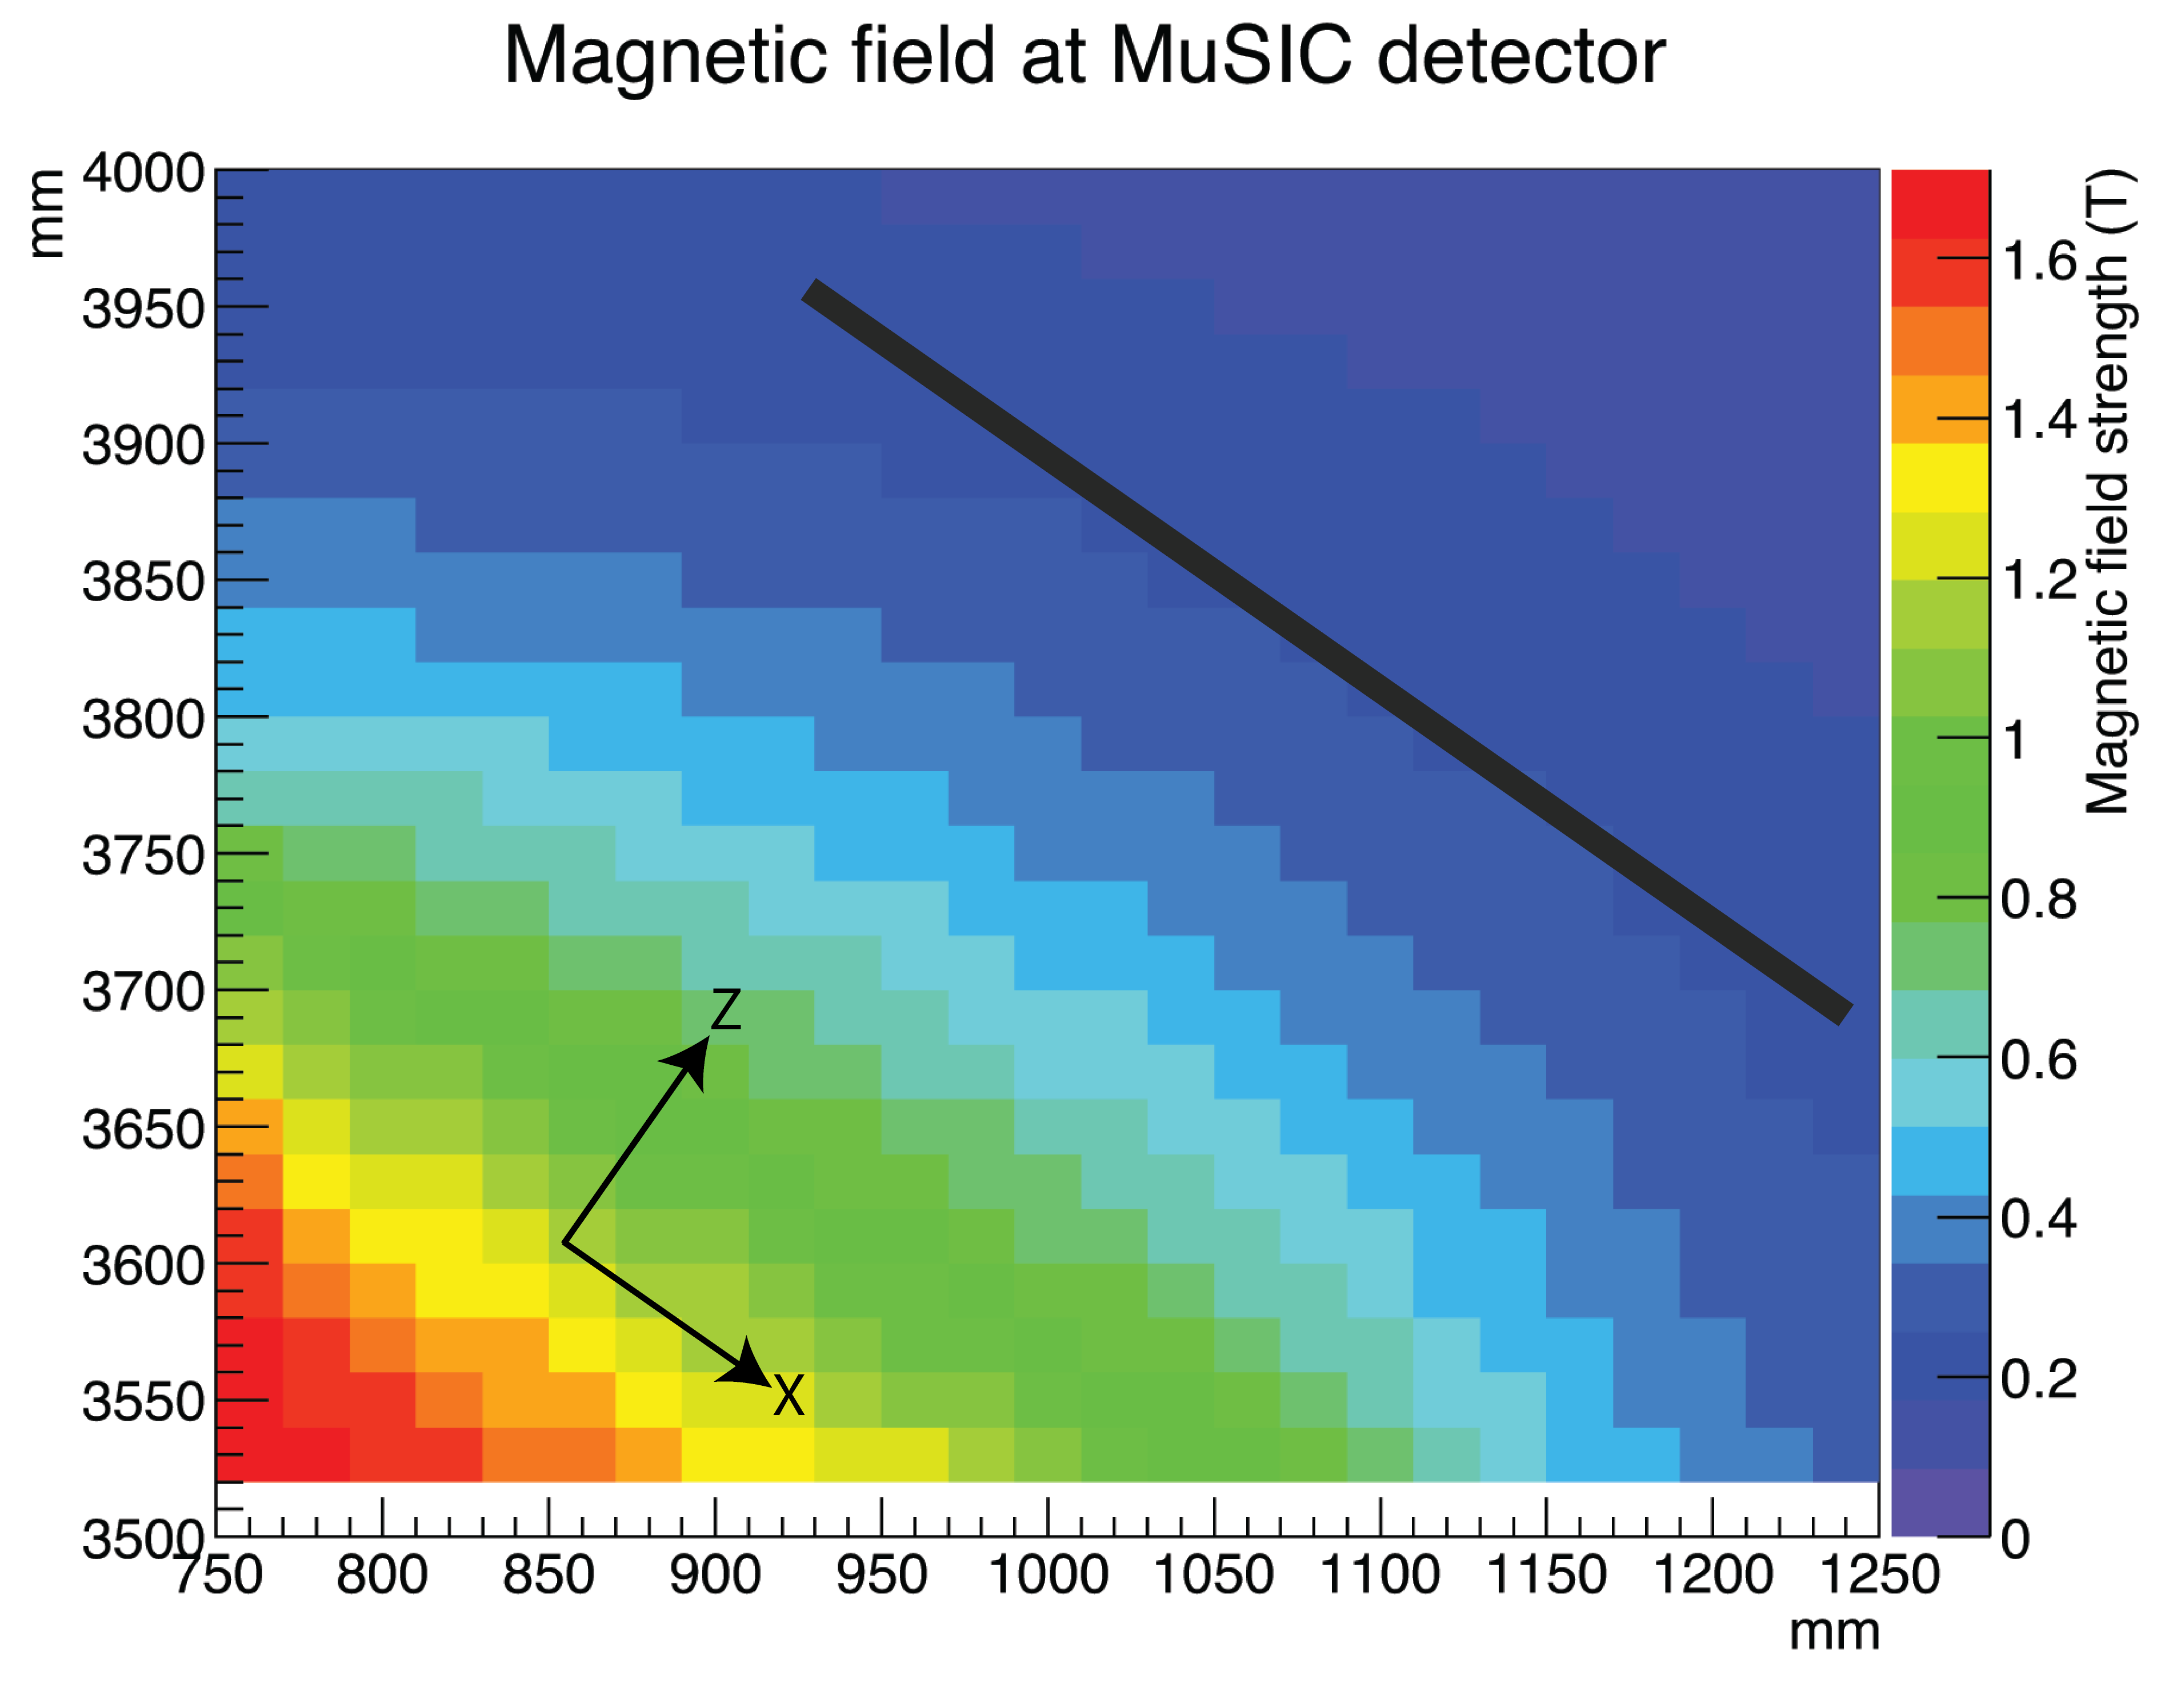
\includegraphics[width=.8\textwidth]{images/field_map_edited.png}
  \caption{The magnetic field strength for the region of interest. The black bar marks the position of the scintillators and stopping target.}
  \label{fig:images_field_map_edited}
\end{figure}

\subsubsection{Stepping Action} % (fold)
\label{sub:stepping_action}
Geant4's stepping action was used to record the status of the simulation. The stepping action is called for every step a particle makes along its track. Using this, steps of interest were written to a ROOT file for later analysis. Two sets of data were recorded: the `truth' data and the `MPPC' data. The truth data recorded every charged particle in any of the core detector components: the degrader, the scintillators, and the stopping target. The data recorded was:
\begin{itemize}
  \item Particle type
  \item Position
  \item Momentum
  \item Time since the start of the event
  \item Which detector component the particle was in
  \item Track ID
  \item Parent particle's track ID
\end{itemize}

The MPPC data attempted to more closely approximate the actual data produced by the detector. This was done by logging photons that were found in an MPPC volume, unlike the truth data where particles were recorded if they were in the scintillator at all (i.e.\  could conceivably be detected). To reduce the overhead of running the simulation only the time and position of the photon were recorded.

% In the MPPC data photons that were found an MPPC were recorded but to keep run time down only the position and time of the step were recorded. Using the position was possible to reconstruct which MPPC detected the photon.

% chapter physics_simulation (end)
%%%%%%%%%%%%%%%%%%%%%%%%%%%%%%%%%%%%%%%%%%%%%%%%%%%
\section{Simulation Analysis} % (fold)
\label{cha:simulation_analysis}

As well as providing a method to test the affects of different detector constructions the Geant4 simulation was also used to verify the analysis technique used in the final measurements.

To aid this analysis a very large numbers of muons were needed (both positive and negative). Given that the G4BL data set only contained 95,420 muons an approximation to the G4BL output was used to test the analysis technique. To approximate the G4BL output gaussian distributions of the muons' position and momentum were used. This was not used for comparison to the data as the approximation was too poor but it was a useful tool to test the analysis method discussed below.

% This was done using an approximate particle distribution rather than the G4BL results. The approximation was used as it was possibly to generate very large sets of data for testing. The large data sets were particularly useful for testing the analysis technique with negative muons which the G4BL distribution was low in. Unfortunately the approximation was not accurate enough to be a substitution for full simulation of the beam done using G4BL.

 % As has been noted attempts to approximate the particle distribution produced by G4BL produced significantly different momenta distributions. The approximations could be used to test the accuracy of the integration technique used to estimate the number of stopped muons, this was especially useful for the stopped negative muons which were much less common in the initial G4BL distribution.

% In order to have suitable statistical significance a much larger number of muons were required than could be produced using the initial G4BL distribution of particles. Instead an approximation to the G4BL distribution was created and then used. The approximation was not close enough to the G4BL distribution to be used as a base of comparison in measurements of the beam but provided a reasonable number of positive and negative muons upon which analysis techniques could be tested.

The core analysis technique used was to create muon lifetime distributions, fit them with a function and then use the integral of the appropriate portion of the function to calculate the number of muon decays that had occurred. This method could be used because no other constituent of the beam would have a lifetime comparable to that of the muons: electrons and protons are stable whilst charged pions have a lifetime of \(26.003\pm0.005\)~ns~\cite{pdg} which is suitably short, even compared to muonic copper, to have little impact on the muon decay spectrum (neutral pions have a lifetime of \( 8.52\times10^{-8}\)~ns and don't produce charged daughters).

The first step of the protocol was to create histograms of downstream\(-\)upstream hit times. In the measurements this was done by an item of hardware but for the simulation this was done by looking for muons in the upstream counter and their daughter-electrons in the downstream counter. The difference in times was then binned, any differences of less than 50~ns were ignored as this was a region that we were blind to in the experiment.

During verification a variety of bin widths were tested in an attempt to minimise the error on any one bin whilst aiming to avoid loss of signal. The was especially important for fitting the copper component of the decay spectrums as this is significant contribution for only the first few bins. Ultimately bin widths of 16~ns were settled on.

The simulation was then fitted using a double exponential: 
\begin{align}
    N_{cu}\exp(-t/\tau_{cu}) + N_{f}\exp(-t/\tau_{f}). \label{equ:dbl_exp}
\end{align}
As the simulated data was pure the background terms used in the final analysis (see section~\ref{sec:momenta_results}) were not included. Using the same method as the experimental technique the values of \(\tau_{cu}\) and \(\tau_{f}\) were fixed at their measured values (163.5~ns and 2,197~ns respectively) for the fitting. Unlike the previously fitted data (figure~\ref{fig:images_mu-_lifetime_in_cu_modded_g4}) the large number of positive muons overwhelm the effect of negative muons captured by air. The fitted values for equation~\eqref{equ:dbl_exp} were extracted into individual exponentials and integrated over the region 50~ns to 20~\(\mu\)s. 

The integrated approximation to the number of decays could then be compared directly to the counted number of muon decays in the simulation. The results of the integration method compared to the counted number of decays are given in table~\ref{tab:sim_counts_vs_integrals}. As can be seen from the table there is good agreement between the counted number of decays and the number produced by the integration method. This verifies the use of the integration method which is the simplest method of estimating the number of muon decays and the only method that can be used with this data.
 \begin{table}
  \begin{center}
  \begin{tabular}{c | c | c | c | c | c}
    Degrader  & Thickness  &  \multicolumn{2}{c|}{Free component}    &  \multicolumn{2}{c}{Copper component}      \\ 
    Material  &    (mm)    &    Count           & Integral           &    Count        &  Integral      \\ 
    \hline
    Air       &      5     &  11722\(\pm\)108   &  11613\(\pm\)119   &  881\(\pm\)30   &     965\(\pm\)58      \\ 
    \hline
    \multirow{4}{*}{Al} 
              &    0.5     &  11827\(\pm\)109   &  11789\(\pm\)119   &  837\(\pm\)29   &     852\(\pm\)57      \\ 
              &      1     &  11723\(\pm\)108   &  11739\(\pm\)118   &  891\(\pm\)30   &     852\(\pm\)56      \\ 
              &      5     &   7078\(\pm\)84    &   7079\(\pm\)92    &  453\(\pm\)21   &      441\(\pm\)42     \\ 
    
  \end{tabular}
  \end{center}
  \caption{Comparison of integrated numbers of muon decays to the counted number of decays in simulation of \(5\times10^5\) initial muons. The free and copper components of the fit were considered separately. The results are for negative muons only as the positive muons only have the free muon lifetime.}
  \label{tab:sim_counts_vs_integrals}
\end{table}


%%%%%%%%%%%%%%%%%%%%%%%%%%%%%%%%%%%%%%%%%%%%%%%%%%%
% The simulation was used primarily to guide decisions on the detector construction but it also aided in testing analysis techniques for the final data. Using the simulated data it was possible to verify that fitting the data and then integrating the fitting function was an effective way of calculating the number of muon decays.
% 
% To carry out accurate fitting a large number of muons were required in the final data so the G4BL produced initial distributions couldn't be used. Instead of the G4BL distribution gaussian approximations to the muon distributions were used. Using the fitted distributions allowed 500,000 initial muons, both positive and negative, to be simulated; this is in contrast to the 86,710 and 9,009 muons (positive and negative respectively) produced by G4BL. 
% 
% The data produced from the Geant4 simulation was fitted using a simple double exponential: 
% \begin{align}
%     N_{cu}\exp(-t/\tau_{cu}) + N_{f}\exp(-t/\tau_{f})
% \end{align}
% This function could then integrated over the fit region (50~ns to 20~\(\mu\)s) to estimate the number of decays. Whilst this was not the final function used to fit the real data the simulation lacks the noise of the real. The counts were carried out by looking at each event for muons in the upstream scintillator and their daughter electrons in the downstream scintillator. Mother-daughter pairs of muons and electrons with a recorded time-at-scintillator of greater than 50~ns were then counted. The comparison of the integrated decay counts and the actual counts can be seen in table~\ref{tab:sim_counts_vs_integrals}. 
% 
% \begin{table}
%   \begin{center}
%   \begin{tabular}{c | c | c | c | c | c}
%     Degrader  & Thickness  &  \multicolumn{2}{c|}{Free component}    &  \multicolumn{2}{c}{Copper component}      \\ 
%     Material  &    (mm)    &    Count           & Integral           &    Count        &  Integral      \\ 
%     \hline
%     Air       &      5     &  11722\(\pm\)108   &  11613\(\pm\)119   &  881\(\pm\)30   &     965\(\pm\)58      \\ 
%     \hline
%     \multirow{4}{*}{Al} 
%               &    0.5     &  11827\(\pm\)109   &  11789\(\pm\)119   &  837\(\pm\)29   &     852\(\pm\)57      \\ 
%               &      1     &  11723\(\pm\)108   &  11739\(\pm\)118   &  891\(\pm\)30   &     852\(\pm\)56      \\ 
%               &      5     &   7078\(\pm\)84    &   7079\(\pm\)92    &  453\(\pm\)21   &      441\(\pm\)42     \\ 
%     
%   \end{tabular}
%   \end{center}
%   \caption{Comparison of integrated numbers of muon decays to the counted number of decays in simulation of \(5\times10^5\) initial muons. The free and copper components of the fit were considered separately. The results are for negative muons only as the positive muons only have the free muon lifetime.}
%   \label{tab:sim_counts_vs_integrals}
% \end{table}
% 
% % chapter simulation_analysis (end)
% % part simulation (end)
% %%%%%%%%%%%%%%%%%%%%%%%%%%%%%%%%%%%%%%%%%%%%%%%%%%%

    \chapter{Characterising the beam} % (fold)
\label{prt:characterising_the_beam}
\section{Introduction} % (fold)
\label{cha:introduction}
Characterisation of the MuSIC beam was carried out over two years and through a number of experiments. Over the course of two years there were five runs making three significant measurements to characterise the beam: the total charged particle flux; the muon flux (by measuring the muon lifetime); and the muon momentum spectrum. The details of the runs are covered in table~\ref{tab:summary_music_beam_time} along with which experiments were carried out. Several other experiments were also carried out by other groups but these are not discussed here (e.g.\ neutron flux measurements and Mo muon-bombardment experiment).
\begin{table}[htpb]
  \begin{center}
    \begin{tabular}{c|c|c}
      \multicolumn{2}{c|}{Dates}          & Measurements                                \\
      Start            & Stop             &                                             \\
      \hline                                                                             
      29 July 2010     & 31 July 2010     & Charged particle flux.                      \\
      \hline
      \multirow{2}{*}{13 February 2011}
                       & \multirow{2}{*}{16 February 2011}
                                           & Charged particle flux.                     \\
                       &                   & Muon lifetime.                             \\
      \hline
      \multirow{2}{*}{19 July 2011}
                       & \multirow{2}{*}{21 July 2011}
                                          & Muon lifetime.                              \\
                       &                  & Muon yield (via muonic X-rays).             \\
      \hline
      22 October 2011  & 23 October 2011  & Neutron flux.                               \\
      \hline
      \multirow{3}{*}{18 June 2012}
                       & \multirow{3}{*}{22 June 2012}    
                                          & Muon momentum spectrum (via lifetime).      \\
                       &                  & Muon yield (via muonic X-rays).             \\
                       &                  & Mo muon-bombardment.                        \\
    \end{tabular}
  \end{center}
  \caption{A summary of the five MuSIC beam-times with notes on the measurements made.}
  \label{tab:summary_music_beam_time}
\end{table}

This chapter has been split into four sections: the rest of this section will be an introduction to the equipment used for the measurements, with each of the three measurements then treated individually. Each measurement section will cover the set up, the results and analysis of the data.

\subsection{Scintillators Preparation} % (fold)
\label{sub:scintillator_preparation}
As discussed in chapter~\ref{prt:introduction}, scintillating materials produce light when charged particles travel through them. There are several categories of scintillator, those used for our measurements were plastic as they are easy to work with, inexpensive and available in a range of sizes. There are two main considerations in preparing a plastic scintillator: maximising light collection and preventing external light contamination. The standard approach to deal with both of these considerations is to polish and wrap the scintillator.

The scintillator surface is highly vulnerable to damage either through scratches or grease. Damage to the surface of the scintillator is problematic as it inhibits light collected through total internal reflection (TIR). Anything that reduces the amount of TIR increases the amount of light absorbed outside of the scintillator, where it cannot be detected. In order to prevent scratches, scintillators must be handled carefully and protective films are only removed at the last moment. As well as careful handling, the scintillators are cleaned to remove dirt and dust by polishing them with iso-propanol, this removes grease that can also degrade the surface.

Scintillators are generally wrapped with two thin layers: an inner reflective material and an outer blackout material. The inner layer is normally aluminium-mylar or foil, this is wrapped loosely in order to leave a small air gap that has been shown to increase the amount of TIR (and hence light collection). The outer layer is normally a black plastic wrap. This is carefully sealed with tape to prevent light leakage (another aid to this is obviously turning any lights off in the experimental area). An important consideration is to keep the layers as thin as possible in order to minimise energy deposition; to this end overlaps are kept to a minimum.

In order to attach sections of the scintillators together and to attach detectors to the scintillator optical cement and grease were used. Optical cement was used when a permanent fixing was required while grease was used if the components would need to be separated. To use the cement the components were cleaned using iso-propanol, then the two-part glue mixed and applied. A foam jig was used to hold the pieces in place whilst the cement set. When non-permanent joins were required, e.g.\ to attach MPPCs to WLS-fibres, optical grease was used to form the connection. Optical cement and grease have refractive indexes close to (if not the same as) that of the scintillators to maximise transmission either between sections of the scintillator (e.g.\ from the scintillator bulk to the WLS-fibre) or from the scintillator to the MPPC.
% Whilst a significant proportion of scintillator construction is dedicated to increasing reflection back into the scintillator, at the boundary to the MPPC it must be minimised to maximise the amount of light hitting the MPPC (rather than being reflected back into the scintillator).

% subsection scintillator_preparation (end)
\subsection{Multi-Photon Pixel Counters} % (fold)
\label{sub:multi_photon_pixel_counters}
Multi-Photon Pixel Counters (MPPCs, see figure~\ref{fig:images_intro_MPPC_from_hammamatsu_report}) are highly sensitive devices able to accurately count photons over a wide range of intensities. An MPPC is a small device (normally \( \mathcal{O}(1\times1) \)~mm\(^2\)) made from many Avalanche PhotoDiodes (APD) operated in `Geiger-mode'. Each individual APD is a single pixel within the MPPC. The APDs are connected together so that the MPPC's output is the sum of the outputs of the individual pixels. As can be seen in figure~\ref{fig:images_intro_hamamatsu_mppc_waveform_and_counts} there is clear banding that corresponds to the number of incident photons making counts, accurate to the single photon, obtainable when operating within the MPPC's limitations (see below).
\begin{figure}[hptb]
  \centering
    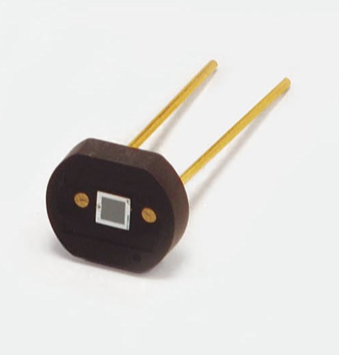
\includegraphics[width=.3\textwidth]{images/intro/MPPC_from_hammamatsu_report.png}
  \caption{Photograph of an MPPC (type S10362-11 with ceramic package) from the Hamamatsu technical report~\cite{hamamatsu_mppc}.}
  \label{fig:images_intro_MPPC_from_hammamatsu_report}
\end{figure}

\begin{figure}[hptb]
  \centering
    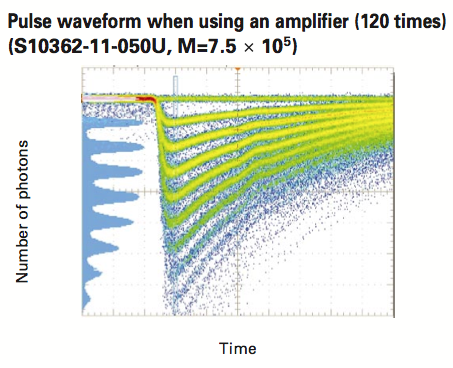
\includegraphics[width=.6\textwidth]{images/intro/hamamatsu_mppc_waveform_and_counts.png}
  \caption{Oscilloscope waveform for an MPPC with a histogram of peak voltage on the left. The histogram shows the clear discrimination between number of photons available on a MPPC. This type of MPPC has \(400\times50\times50 \mu\text{m}^2\) APDs in a \(1\times1\text{mm}^2\) package taken from~\cite{hamamatsu_mppc}.}
  \label{fig:images_intro_hamamatsu_mppc_waveform_and_counts}
\end{figure}

APDs make use of the photoelectric effect and large voltages to produce an `avalanche' of electrons when triggered by an incident photon. A limitation to this system is that an individual APD's output is roughly constant regardless of the number of incident photons. Should the number of photons become comparable to the number of pixels then the MPPC becomes saturated and produces a constant signal as all the pixels fire, rather than clear bands as pixels fire in isolation. For the energy range predicted at MuSIC saturation is not considered to be a significant problem as the number of photons is predicted to be below the one hundred pixels used in our MPPCs (see figure~\ref{fig:sim_n_photons}). 

\begin{figure}[hptb] 
  \centering    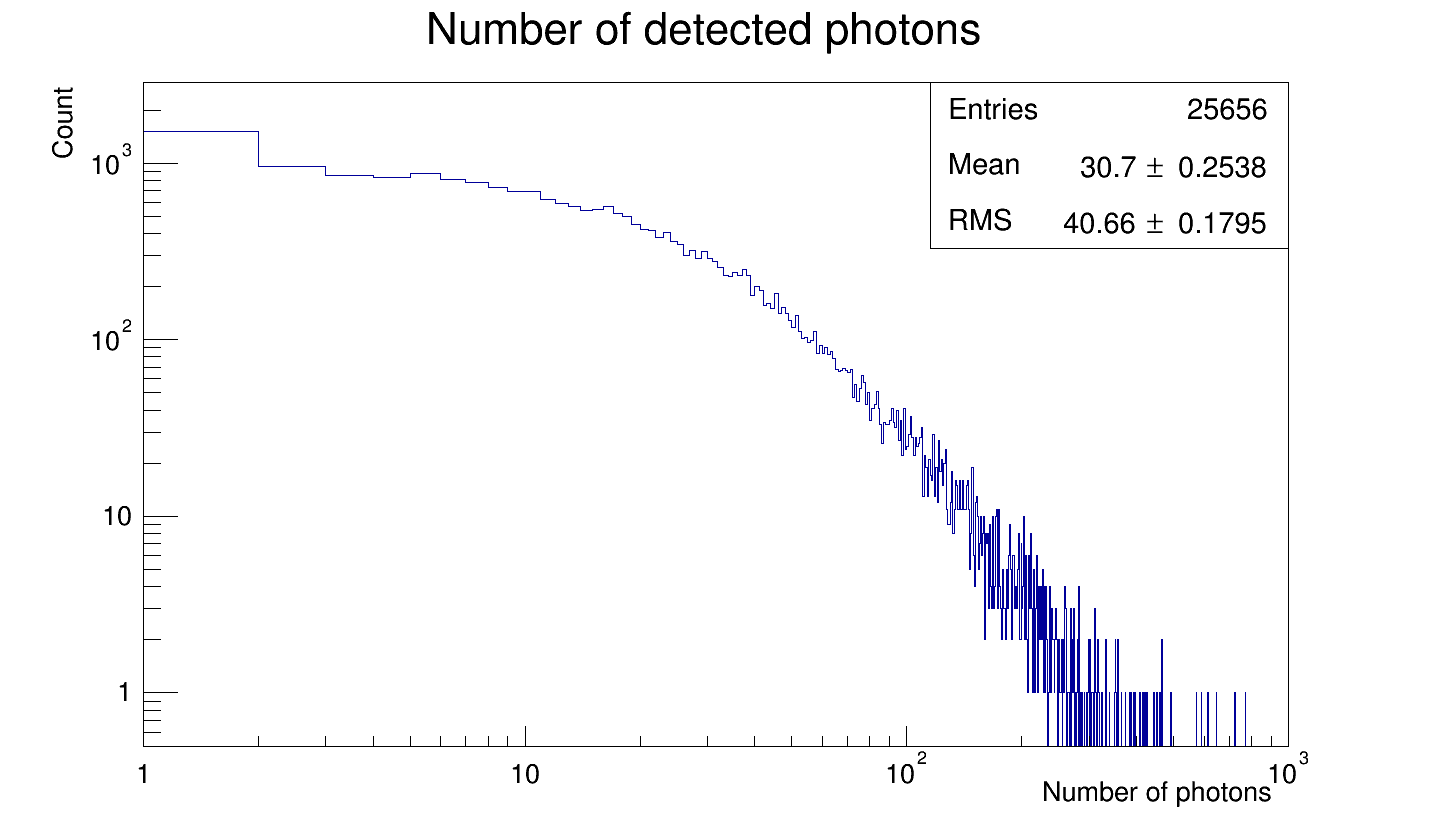
\includegraphics[width=.9\textwidth]{images/plot_generating_scripts/n_photons.png}
  \caption{Simulated distribution of number of photons reaching one of the MPPCs attached, via wavelength shifting fibre, to a \(380\times50\times3.5\)~mm\(^3\) scintillator.}
  \label{fig:sim_n_photons}
\end{figure}


An MPPC has several key attributes: Photon-Detection Efficiency (PDE), peak sensitivity, time resolution, operating voltage (\( V_0 \)), gain (\( M \)) and dark current. The PDE and peak sensitivity respectively describe the likelihood of detection of a photon of given wavelength (see figure~\ref{fig:images_intro_hamamatsu_pde_vs_wavelength}) and the wavelength that the MPPC is most sensitive to (typically \(\sim\)440~nm). Time resolution for MPPCs is generally very good, normally 200--300~ps for FWHM at the single photon level which is more than accurate enough for our purposes. The operating voltage is the potential required to make the MPPC work, due to variance in manufacture this is given individually for each MPPC and has to has to be set correctly for optimum performance, Hamamatsu's MPPCs have \( V_0 = 70\pm10 \)~V. The gain of the MPPC indicates the strength of the signal response to a photon, typical values are between \( 10^5 \) and \( 10^6 \), this corresponds to signals of \( \mathcal{O}(1\text{--}10) \)~\(\mu\)V which must be amplified for accurate measurement. The dark current is a measure of how noisy a particular MPPC is; it is the rate of false signals that have an effective strength equivalent to 0.5~photo-electron (p.e.). Typical values for the dark current are in the range 100--500 kcps (\(\times10^3\)~counts per second) these can be accounted for by correct setting of triggers.
\begin{figure}[hptb]
  \centering
    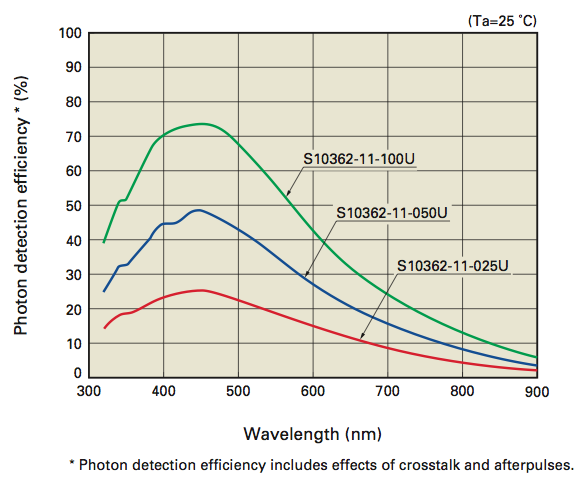
\includegraphics[width=.5\textwidth]{images/intro/hamamatsu_pde_vs_wavelength.png}
  \caption{MPPC Photon Detection Efficiency (PDE) as a function of photon wavelength. A range of pixel densities are shown (100, 400, 1600 pixels/\( 1\times1\text{mm}^2\) for the 100U, 050U and 025U models respectively). Taken from~\cite{hamamatsu_mppc}.}
  \label{fig:images_intro_hamamatsu_pde_vs_wavelength}
\end{figure}

As can be seen, whilst MPPCs have many useful features they do have several features that need careful treatment to make them useful: mainly amplification and noise reduction. These two problems are closely related and in fact, when treated properly one will often help with the other. Given the size of the signal from an MPPC it is obvious that amplification is required to make the signal useable, in fact, as will be discussed below, an unfiltered MPPC signal is too small for detection by most standard equipment. Amplification is done using linear amps which are applied as soon as possible to reduce noise due to cabling as well as attenuation. 
% As well as amplification simple filters are applied to the bias voltage and signal to help reduce noise (see figure~\ref{CIRCUIT DIAGRAM}). Careful ground was also required to reduce noise, this was mainly carried out by ensuring shared ground between different modules.

% subsection multi_photon_pixel_counters (end)
\subsection{Secondary Emission Chamber} % (fold)
\label{sub:secondary_emission_chamber}
As well as studying the resultant beam, knowledge of the initial proton beam is essential for normalisation. This is done using a Secondary Emission Chamber (SEC). A SEC uses thin foils of gold placed within a strong electrical potential. When protons pass through the foils a small number of electrons are produced as part of ionisation, these can then be collected and counted. The SEC only measures a fraction of the beam and even then, only indirectly. In order to calibrate the SEC, runs are performed in which the entire proton beam is absorbed with a copper block downstream of the SEC. Measurement of the total current produced by the block can then be used to determine the fraction absorbed by the SEC, and hence the conversion factor. Measurement of the SEC was carried out using scalers (see below) that counted the cumulative charge passing through the SEC.

% subsection secondary_emission_chamber (end)

\subsection{NIM, CAMAC and VME} % (fold)
\label{sub:nim_and_camac}
Rather than develop custom data acquisition hardware, a modular crate system was used. A crate system supplies power and mechanical fixings for a range of modules, these modules can then be connected together to produce a system. Three crate systems were used: Nuclear Instrument Module (NIM), Computer Automated Measurement And Control (CAMAC) and Versa Module Eurocard bus (VMEbus or VME). NIM supplies power only, whilst CAMAC and VME provide a `backplane' through which data can be transferred to a control card.

NIM modules were primarily used to provide signal processing and data acquisition logic. The CAMAC and VME crates were used for data read-out. Ultimate control and storage was carried out using a PC which recorded the data for later analysis. The rest of this section will discuss the basic modules used in NIM, CAMAC and VME.
\subsection{Discriminators} % (fold)
\label{ssub:discriminators}
A discriminator works by producing a digital signal when an analogue input signal exceeds some preset threshold. Converting the analogue signal to digital makes it much easier to manipulate as many other modules can only use a digital signal. The discriminators were powered by NIM modules and had their thresholds set manually.

Discriminators were used to signal when a certain number of photons were detected by an MPPC i.e.\ when a particle had passed through the scintillator. As the discriminators have a minimum threshold of \(\sim\)25~mV the MPPC signals were amplified to make them useable. As every MPPC has a different gain the thresholds for the discriminators had to be set individually. To normalise between MPPCs the discriminator thresholds were set based on the number of photons the analogue signal corresponded to (see figure~\ref{fig:images_intro_hamamatsu_mppc_waveform_and_counts}). The trigger level (in p.e.)\ was the same for all MPPCs and was chosen to maximise the signal to noise ratio, a typical value was \(\sim2.5\)~p.e.\ which suppressed most of the dark current without compromising sensitivity to charged particles. An oscilloscope could then used to translate the photon (p.e.)\ threshold into a voltage threshold (in mV) that can be used by the discriminator.

% The thresholds had a standard minimum value of \(\sim\)25~mV, in order to meet this linear amplifiers were used to boost the MPPC signal enough to be detectable. 

% subsubsection discriminators (end)
\subsection{Gates and Latches} % (fold)
\label{ssub:gates}
Gates are a set of modules that generally have several related functions. Depending on the mode they can change the length of a signal, delay it, `latch' it or start a clock signal. The first two modes are generally used for creating `gates' (on or off signals) for other modules: e.g.\ turning on a module to record the shape of a signal or indicating to the PC that their is data waiting to be read. A `latch' is a signal that remains on until another signal switches it off, these are often used when it's unclear how long something will take e.g.\ sending data to the PC. Clock signals were generally used as calibration information for other measurements e.g.\ recording the SEC.

% Gates are modules that, when triggered produce an altered signal compared to the input. As well as delaying and lengthening signals gates can also be used in `latch' (or flip-flop) mode. Gates only accept digital signals but can create delays of up to 1~s, and equally change the length by similar amounts. In latch mode the input signal starts the output whilst another input resets it. Latch mode is used to create busy signals by using the input to indicate when the DAQ is processing an event and a signal from the PC to reset it.

% subsubsection gates (end)
\subsection{Logic units} % (fold)
\label{ssub:logic_units}
Logic units provide boolean logic (`AND', `OR', `NOT') for processing digital signals. The limiting factor is the number of inputs that can be combined and the complexity of the combinations. Normally signals are combined in a block with a single module having several discrete blocks. Each block will perform a single logical operation (OR or AND) on its inputs. The inputs of a block can either be normal or negated. A block (or sometimes the entire module) will generally have a veto signal that will stop outputs until the veto is cleared.

Logic units were generally used for simple tests such as checking that all MPPCs on a scintillator had triggered, this helped reduce the number of false positives in addition to the application of a discriminator. Logic units were also used to prevent attempts to process two events at once: if a second event arrived before the previous event was fully processed then the second event was ignored. This leads to `dead time' but is unavoidable.

% subsubsection logic_units (end)
\subsection{Scaler} % (fold)
\label{ssub:scaler}
A scaler is a counting module. It receives a digital input, that when asserted, increments its counter. The most important factor of a scaler is its maximum speed (the maximum input frequency). Events that occur more rapidly than the input frequency will not be properly counted (either not being counted at all or counted as a single event), a typical maximum input frequency is 100~MHz. Most scalers can be daisy-chained together in case their maximum value is exceeded and some allow multiple inputs that can be counted independently. NIM scalers will generally be read-out by eye (e.g.\ using a display) whilst VME/CAMAC modules will be read-out using the crate's data-bus. 

% One of the simplest forms of read out is a count of triggers, this is what a scaler does. The primary concern with a scaler is the input specification to trigger a count as well as the maximum speed at which the unit can count. Modules can either be used with NIM, CAMAC or VME. When the rate is high or the maximum count is low multiple scalers can be daisy-chained together to provide carry over. 

% subsubsection scaler (end)
\subsection{Analogue to Digital Converter} % (fold)
\label{ssub:analogue_to_digital_converter}
There are two primary attributes of an MPPC signal that were measured: its size and its separation from other signals. In order to measure the size of the MPPC signal, an Analogue to Digital Converter (ADC) was used. ADCs work in a variety of ways depending on the exact type of measurement they are making, two common versions used at MuSIC were Peak Sensing ADC (PS-ADC) and Charge-integrating ADCs (QDC). Both types of ADC measure a component of the input analogue signal, the PS type measures the peak voltage whilst the QDC measures the integrated charge, both make these measurements only when enabled by the ADC's `gate'. The ADC's gate is normally set to be slightly longer than the expected signal from an MPPC, i.e.\ \( \sim \)50~ns. 

Several factors define the ADC: the number of bits it is able to read out, the range of input signals that it can measure, its linearity, digitisation/read time (`dead time') and number of channels. The number of bits the ADC has, the range and its linearity work together to determine the accuracy of the ADC; the number of bits determines the resolution between any two values, the range determines the values that the ADC can measure whilst the linearity maps measured values to actual voltages. Dead time measures how long is required to measure the analogue signal and how long it takes to then send the digitised values to the controlling PC i.e.\ for how long the module is inoperative, `dead'. The number of channels on an ADC is a measure of how many inputs it can measure simultaneously, normally one is ascribed to each MPPC so that the triggering signal can be recorded.

A key feature of using an ADC is the pedestal, obviously any analogue signal is going to have some noise that represents its zero level, in an ADC this manifests as a large peak in the lower bins of the ADC, removal of the pedestal is often done by the ADC itself and through the DAQ but it does sometimes have to be removed from the data as well.

% subsubsection analogue_to_digital_converter (end)
\subsection{Time to Digital Converter} % (fold)
\label{ssub:time_to_digital_converter}
A Time to Digital Converter (TDC) measures the time difference between signals. The core parameters for a TDC are the number of bits of precision on each channel, the maximum duration the TDC can record, its linearity, its dead time and number of channels of input. A TDC measures time between a `start' and a `stop' signal. Normally a single start signal is provided to the entire TDC with each channel receiving a stop signal. The measured times between the global start signal and the individual stop signals are then read-out independently. 

An alternative TDC used in later experiments is the Multi-Hit TDC (MH-TDC). Rather than measure a single start/stop pair for each channel the MH-TDC has a ring-buffer to record data for each channel. A ring-buffer has a fixed length (the `window'), typically \(\mathcal{O}(50)\)~\(\mu\)s, when a signal (a `hit') is received its position within the window is marked. The ring-buffer records every hit it receives, regardless of the start signal. When the start signal is received the buffer is read-out, this can be done immediately or after a delay. By using a delay signals both before and after the start signal can be recorded.

 % When the `start' signal is received it signals that the current state of the buffer (and some trailing amount) should be recorded. Using this method, events proceeding the start signal can be recorded as well as those afterwards.

% subsubsection time_to_digital_converter (end)
\subsection{Registers} % (fold)
\label{ssub:registers}
Registers are modules that allow simple logical signals to be sent to or from a PC. In our systems they have two key uses: either indicating to the controlling PC that there is data to be read (an `interrupt') or for the PC to indicate that all the data has been read and that the DAQ should be reset. The interrupt time had to be carefully delayed such that there was long enough for the digitisation to complete whilst minimising dead time. The DAQ reset signal was sent by the PC once it had read all the modules to indicate that data taking could resume.

 % Interrupts were formed using a logic unit and a gate: once a trigger had be formed by the logic unit the gate would delay the interrupt signal long enough for the ADC and TDC digitisation to complete then signal the controlling PC. The PC's reset signal was used to unlatch the veto signals that prevented doubling up of data as well as clear any other latches used by the system.

% Control registers are fairly simple devices but very useful in general control, they act as a simple toggle that can either send or receive a signal to the controlling PC. The main use of registers is to form an interrupt; used this way once data has been taken the ready state of the system can be signalled to the PC and the PC can begin read-out. The interrupt is often delayed so that full digitisation can occur although has to be carefully gauged to prevent excessive dead time. The second common use is to reset the system once read-out has completed, this normally means resetting a latched gate that has been holding the system in veto.

% subsubsection registers (end)
% subsection nim_and_camac (end)
% section experimental_technique (end)
\clearpage
% chapter introduction (end)
\section{Charged Particle Flux} % (fold)
\label{cha:charged_particle_flux}
% TODO Pictures of set ups
% TODO Diagrams of set ups
The first experiment carried out at MuSIC aimed to measure the total flux of charged particles. As well as this measurement it was also a test-bed for the technology and techniques used in later experiments.

Two separate measurements of the charged particle flux were made: one using a long strip scintillator that measured the flux at a range of vertical positions and a second that used a smaller disk that measured the flux at a number of points across the face of the disc.

The DAQ used for these experiments was designed to have a lot greater functionality than was ultimately used. The original design aimed to use the difference of arrival times at the various MPPCs for greater positional accuracy whilst the ADC measurements were intended to measure the energy of the particle; neither of these techniques were successful but the full DAQ is included for completeness.

% These early experiments had DAQ designs that were ultimately superfluous as the data it yielded was not used; this design is included for completeness.
\subsection{Experimental Set Up} % (fold)
\label{sec:experimental_set_up}
The experimental design for both measurements was broadly the same: the scintillators both had four MPPCs attached. In the first measurement a long strip scintillator was used and the MPPCs were distributed evenly across the short ends, for the second measurement the disk had the four MPPCs placed evenly around the circumference (see table~\ref{tab:charged_particle_flux_scint_details}). NIM crates housed the modules for the triggering logic, digitisation was performed via CAMAC modules and the read out data was recorded on a PC to be analysed afterwards. The scintillators were both wrapped with aluminium foil and black wrap and the MPPCs attached via optical cement. The scintillators were mounted on aluminium supports at the end of the beam-pipe.
\begin{table}[hptb]
  \begin{center}
    \begin{tabular}{c|c|c|c}
      Shape  &  Volume (mm\(^3\))           &  MPPCs  &  MPPC positions                    \\
      \hline
      Strip  &  \(380 \times30\times10\)    &  4      &  \( \pm 5 \)~mm on each end.       \\
      Disk   &  \( 35^2\times\pi\times20\)  &  4      &  Radially, every 90\( ^{\circ} \). \\
    \end{tabular}
  \end{center}
  \caption{Details of the scintillators used for the two measurements of the charged particle flux.}
  \label{tab:charged_particle_flux_scint_details}
\end{table}

The aim of these early experiments was to make three measurements: the total trigger rate, the difference in arrival times of light at the MPPCs and the distribution of the number of firing pixels at each MPPC. The total trigger count is proportional to the flux of charged particles through the scintillator. The timing and photon counts were hoped to give information on positioning and the amount of energy deposited but this was found to be incorrect.

% It was hoped that the timing difference between MPPC firings could be correlated to the position of the interaction within the scintillator (this was ultimately incorrect). The distribution of the number of firing pixels was hoped to give some idea of the energy deposited, and possible the types of particles. 

Ultimately only the measurement of the trigger rate was successful. The trigger rate is proportional to the charged particle flux,  assuming negligible dead time. To ensure a negligible dead time, as discussed below, a simplified DAQ system was used and MuSIC was run with a reduced beam current (\(<1\)~nA instead of the MuSIC design current of \(~1\)~\(\mu\)A). Another concern for measuring the charged particle flux are minimally ionising particles (MIPs). MIPs, by definition produce a minimal amount of scintillation light, making their detection difficult. The thickness of the scintillators, especially the second (20~mm) should still be sensitive to MIPs.

% to mitigate this a thicker scintillator (20~mm) was used for the second measurement in which more energy would be deposited.

The DAQ used to measure the trigger rate was a subset of the full DAQ, used to measure the time and energy:
\begin{enumerate}
  \item Amplify the MPPC signal to a detectable level.
  \item Remove dark current using a discriminator.
  \item Create a trigger and veto from the coincidence of all MPPCs: an `AND' operation applied to the output of the discriminators.
   % logic module to form a trigger (further removing noise) and raise a veto based on the coincidence of events from all MPPCs.
  \item Record the analogue MPPC signal using an ADC.
  \item Use the trigger and the first MPPC's signal to start the TDC.
  \item Delay three of the remaining signals to form the stops to the TDC (the delay can be removed to regain the accurate time).
  \item Remove the veto on the system once read-out is complete.
\end{enumerate}
This can be seen as a schematic in figure~\ref{fig:MuSIC1_DAQ_Block}. 

\begin{figure}[hptb]
  \centering
  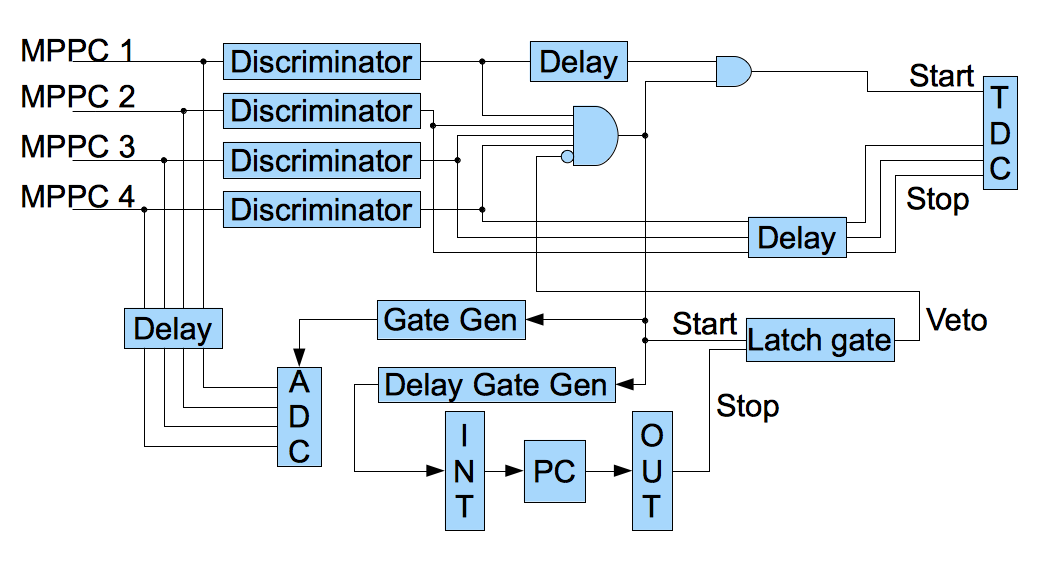
\includegraphics[width=.9\textwidth]{images/charged_flux/MuSIC1_DAQ_Block.png}
  \caption{Schematic of the DAQ used for measuring the charged particle flux. Horizontal blocks indicate NIM units whilst vertical units were mounted in a CAMAC crate. The two `AND' blocks were made using NIM modules.}
  \label{fig:MuSIC1_DAQ_Block}
\end{figure}

To make the final measurement of the trigger rate, the majority of the DAQ was ignored and the four-fold coincidence counted using a scaler. By counting the raw triggers, effects of dead time could be negated and a truer value for the number of interactions obtained. For the 1D experiment, measurements were made over 50~s with control done via hand, this obviously had limitations 

The positions of the two experiments are given in table~\ref{tab:flux_setup} with respect to the centre of the beam-pipe. `By-eye' read-out of the 1D measurement was done using a display mounted on the scaler used to count triggers. For the 2D measurement a CAMAC module was used that was read out by computer. It's important to note that not only were the detectors very different but due to experimental constraints the 2D measurement was made significantly further from the end of the beam pipe than the 1D experiment (85~cm compared to 6~cm).
\begin{table}
  \begin{center}
    \begin{tabular}{c|c|c|c|c|c}
      Measurement  &  \multicolumn{3}{c|}{Distance from centre of beam (cm)}         &  Scaler    &  Read-scout \\
      &    Horizontal    &       Vertical              &  Longitudinal  &  Time (s)  &          \\
      \hline            
      1D           &  0               &  \(-5\), \(-15\), 0, 15, 5  &       6        &  50        & By-eye   \\
      2D           &  \(-17\), 0, 17  &  \(-16\), 0, 20, 25         &       85       &  20        & CAMAC    \\
    \end{tabular}
  \end{center}
  \caption{Positions at which the charged particle flux was measured, 1D refers to the first run in which only the vertical displacement was measured, 2D refers to the second run in which horizontal measurements were also take. The distances from the beam-pipe were 6~cm for 1D measurements and 85~cm for 2D, this was due to mechanical constraints.}
  \label{tab:flux_setup}
\end{table}

% section experimental_set_up (end) 
\subsection{Detector efficiency} % (fold)
\label{sec:detector_efficiency}
As well as making measurements of the charged particle flux another important measurement, made soon after the second beam time, was measurement of the efficiency of the circular detector. This was done using three large (\( 40\times40\times1 \)~cm\(^3\)) scintillator paddles. Light from the scintillators was detected using Photo-Multiplier Tubes (PMT). The three large paddles were positioned sandwiching the circular scintillator, two above and one below. 

The circular detector's efficiency was calculated using the ratio of detections by the PMTs to detection by the MPPCs (once size considerations had been taken into account). It was assumed that the rate of detection by the circular scintillator was proportional to the detection rate in the three large scintillators. The first test was the efficiency of all three remaining MPPCs (one had become irrevocably damaged during beam time) then the efficiency of pairs of MPPCs was tested. Testing consisted of counting the occurrence of three-fold coincidence on the PMTs and either two or three fold coincidence on the MPPCs. Data was taken for approximately one day for each configuration. The MPPCs were not tested individually to ensure that dark current events were not included, although these were reduced by using a discriminator to produce the signals. The results of this measurement are shown in table~\ref{tab:music2_eff}.

\begin{table}
  \begin{center}
    \begin{tabular}{c | c | c | c | c | r@{~\( \pm \)~}l}
      \multirow{2}{*}{Configuration} 
                     &  Run Time             &  MPPC   &  PMT        &  \multirow{2}{*}{Efficiency} 
                                                                                    &  \multicolumn{2}{c}{Adjusted}   \\
                     &  (\(\times 10^3\)~s)  &  Count  &  Count      &              &  \multicolumn{2}{c}{Efficiency} \\
      \hline
      123            &  86.0                 &  1651   &  1,161,165  &  0.00142     &  0.0591 & 0.0015  \\
      12             &  92.3                 &  6055   &  1,229,389  &  0.00493     &  0.2048 & 0.0026  \\
      13             &  87.1                 &  5653   &  1,179,116  &  0.00479     &  0.1993 & 0.0027  \\
      23             &  84.4                 &  3999   &  1,129,137  &  0.00354     &  0.1472 & 0.0023  \\
        
    \end{tabular}
  \end{center}
  \caption{Summary of the data taken for measuring the MPPC detector efficiency. Configuration refers to which of the three MPPCs were tested. The efficiency is the simple ratio of the MPPC count to the PMT count whilst the adjusted efficiency has been scaled by the ratio of the areas of the scintillators, i.e.\ by \( \frac{40\times40}{\pi3.5^2} \).}
  \label{tab:music2_eff}
\end{table}

Assuming that the total efficiency (\( \epsilon_t \)) is the product of the individual efficiencies (\( \epsilon_{1,2,3} \)) then it can be expressed as:
\begin{align}
  \epsilon_t &= \epsilon_1  \epsilon_2  \epsilon_3
\end{align}
With the measured efficiencies of the pairs of MPPCs we can calculate the individual efficiencies by solving:
\begin{align*}
  \epsilon_{12} &= \epsilon_{1} \epsilon_{2} &\implies   \epsilon_{1}  &= \frac{\epsilon_{12}}{\epsilon_{2}}                       \\
  \epsilon_{13} &= \epsilon_{1} \epsilon_{3} &\implies   \epsilon_{2}  &= \frac{\epsilon_{12}\epsilon_{3}}{\epsilon_{13}}          \\
  \epsilon_{23} &= \epsilon_{2} \epsilon_{3} &\implies   \epsilon_{3}  &= \sqrt{\frac{\epsilon_{23}\epsilon_{13}}{\epsilon_{12}}}  \\
\end{align*} 
This can be generalised to:
\begin{align*}
  \epsilon_{i} &= \sqrt{\frac{\epsilon_{ij}\epsilon_{ik}}{\epsilon_{jk}}} \label{equ:individual_eff}
\end{align*}
Where \( \epsilon_i \) is a single efficiency we want to calculate and \( \epsilon_{jk} \) is the combined measurement of the other two efficiencies. Applying this to table~\ref{tab:music2_eff} we get the efficiencies for the MPPCs shown in table~\ref{tab:calculated_individual_eff}. It's important to note that these efficiencies represent more than just the individual MPPC's quantum efficiency but the entire gestalt of systematic effects that contribute to the efficiency of the specific MPPC including scintillator acceptance (both geometric and energetic), light collection and transmission. As can be seen the estimated total efficiency ends up being larger than what was actually measured but this is to be expected as the system assumes all the efficiencies are completely independent of one another. Using these values the average efficiency of a single MPPC can be calculated and given an error as seen in the final line of the table.

\begin{table}
  \lineup
  \begin{center}
    \begin{tabular}{c|r@{~\(\pm\)~}l}
      MPPC  &  \multicolumn{2}{c}{Efficiency} \\
      \hline
      1  &  0.5265 & 0.0064  \\
      3  &  0.3786 & 0.0046  \\
      2  &  0.3889 & 0.0048  \\
      \hline
      \( 123_{Calc} \)  &  0.0775  &  0.0016  \\
      \( 123_{Meas} \)  &  0.0591  &  0.0015  \\
      \hline 
      \( \epsilon_{\text{Ave.}} \)  &  0.431\0 & 0.067 \\
         
    \end{tabular}
  \end{center}
  \caption{Efficiencies of individual MPPCs calculated using the values from table~\ref{tab:music2_eff}, and equation~\eqref{equ:individual_eff}. The two values below the line represent the total efficiency as calculated using the individual values and the measured value. The final value, \(\epsilon_{\text{Ave.}}\) is the mean efficiency of the three individual efficiencies, it's error is the standard deviation of those values. Note: these values include any acceptance effects, the light collection efficiencies of the scintillator and any effects due to the DAQ.}
  \label{tab:calculated_individual_eff}
\end{table}


% section detector_efficiency (end)
\subsection{Results} % (fold)
\label{sec:results}

Prior to the main experiments the conversion factors from SEC count to proton current was determined, these values were determined to be, respectively for the 1D and 2D measurement: 0.03408~nA and 1.514~nA. The results from the measurements are presented in table~\ref{tab:1d_res}, for the 1D case, and table~\ref{tab:2d_res} in the 2D case. The counts were converted to rates and the flux calculated using:
\begin{align}
  j &= \frac{F(C - C_{off})}{I_{p}} \\
  I_{p} &= K(S - S_{off})
\end{align}
where \(j\) is the flux, \(F\) is a scaling factor, \(C\) is the trigger count with the beam on, \(C_{off}\) is the background trigger rate (i.e.\ with the beam off), \( I_{p} \) is the proton current, \(S\) is the SEC count, \(S_{off}\) is the SEC count with the beam off and \(K\) is the SEC to current conversion factor. The scaling factor, \(F\), was used to account for different conditions between runs. \(F\) was taken to be the ratio of the measurements made at the same location. I.e.\ the scaling factor for the 1D case was the ratio of the two measurements made at 0~cm. For the 1D measurement there was a difference between the first four and last five measurements due to damage to the MPPCs (one broke and another became detached from the scintillator). The 2D measurements were made at a larger distance than the 1D measurements as there was another experiment upstream that prevented closer positioning. The upstream experiment was used to make the muon lifetime measurement discussed below, it consisted of two scintillators on either side of stopping target. The stopping target was initially 20~mm of magnesium that was changed to 5~mm of copper for the final 3 runs.


\begin{table}
  \begin{center}
    \begin{tabular}{ r | r | c | c | c | c | r@{~\(\pm\)~}r } 
      Height   &  \multicolumn{2}{c|}{Trigger Count}    &  \multicolumn{2}{c|}{SEC Count}  &  Factor   &  \multicolumn{2}{c}{Flux (\(j\))}          \\
      (cm)     &  \multicolumn{1}{c|}{(\(C\))}  
                             &  (\(C_{off}\))           &    (\(S\))   &   (\(S_{off}\))   &  (\(F\))  &  \multicolumn{2}{c}{(nA\(^{-1}\))} \\
      \hline
        0      &  2,151,736  &    \multirow{4}{*}{30}   &   1,255  &  \multirow{4}{*}{381} &  \multirow{4}{*}{\(1.0\pm0.0\)}  
                                                                                                      &  72,200 & 3,300  \\
      \(-5 \)  &  1,438,685  &                          &   1,286  &                       &          &  46,600 & 2,100  \\
      \(-15\)  &    446,302  &                          &   1,212  &                       &          &  15,770 &   760  \\
      \(-15\)  &    502,596  &                          &   1,208  &                       &          &  17,830 &   860  \\
      \hline            
        5      &  1,663,702  &   \multirow{4}{*}{83}    &   1,298  &  \multirow{4}{*}{398} &  \multirow{4}{*}{\(1.684\pm0.034\)}  
                                                                                                      &  91,300 & 4,000  \\
        5      &  1,420,836  &                          &   1,142  &                       &          &  94,300 & 4,800  \\
       15      &  1,080,170  &                          &   1,336  &                       &          &  56,900 & 2,400  \\
       15      &  1,185,051  &                          &   1,371  &                       &          &  60,200 & 2,500  \\    
       \hline
        0      &  1,307,015  &         34               &   1,298  &             404       & \(1.684\pm0.078\)
                                                                                                      &  72,200 & 3,200  \\
    \end{tabular}
  \end{center}
  \caption{Summary of the results from the measurement of the vertical charged particle flux. The errors are statistical whilst the error on \(F\) is calculated as the errors on the un-scaled measurements at 0~cm added in quadrature. The error on the flux is calculated as the propagated errors of the other values. Counts were taken for 50~s. The SEC conversion factor, \(K\), was 0.03408~nA. The factor was taken to be the ratio of two measurements made at 0~cm. The 0~cm measurements were used as this was the only pair of measurements that were made with the experiment in both conditions (i.e.\ all MPPCs functional and later, with one broken and another damaged).}
  \label{tab:1d_res}
\end{table}


\begin{figure}[hptb]
  \centering
  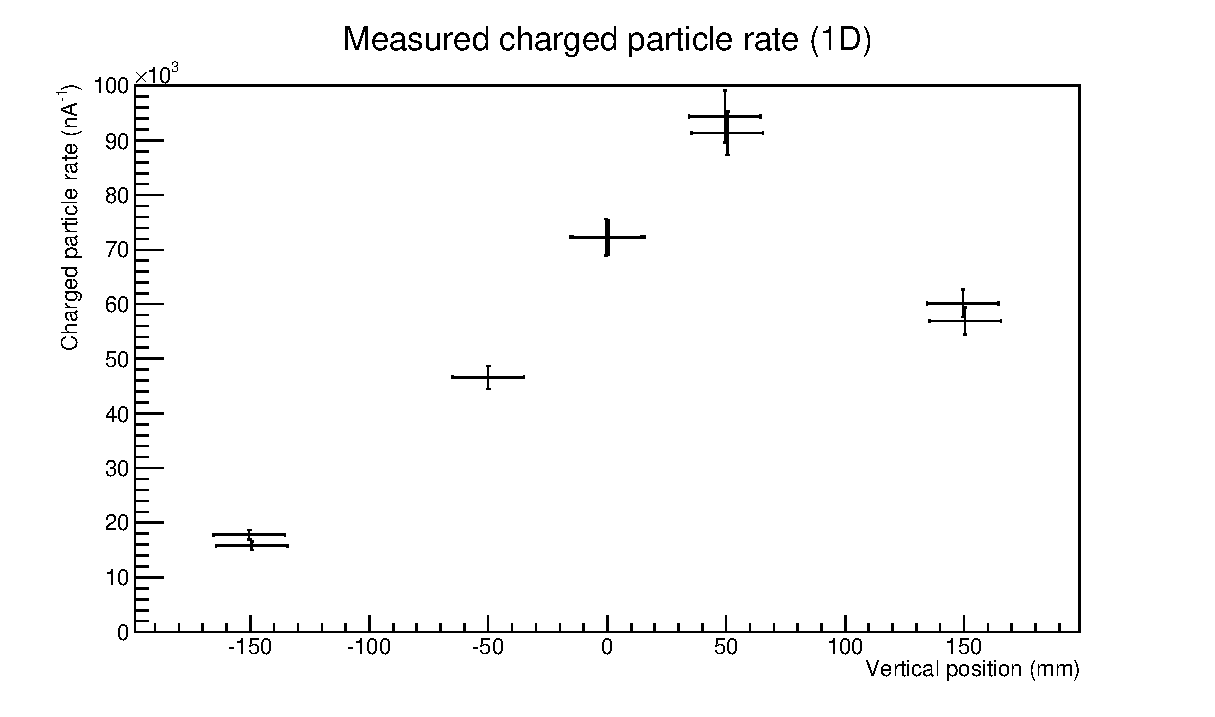
\includegraphics[width=.8\textwidth]{images/plot_generating_scripts/measured_1d_charged_flux.eps}
  \caption{Measurement of the 1D charged particle flux as given in table~\ref{tab:1d_res}. Where two measurements were made at a single location an offset has been applied to the point to allow clearer reading of the plot, the measurements were actually at the same position. The errors on the vertical position are the width of the scintillator used.}
  \label{fig:images_hit_rate_rescaled}
\end{figure}


% Values calculated in https://docs.google.com/spreadsheet/ccc?key=0Ahpo2ep0Rqg5dGNBZk9EZTZmc2w1N0RiR2UwSHZkQ0E#gid=4
% and get_average_hit_rates used to calculate the rates
\begin{table}
  \begin{center}
    \begin{tabular}{r | r | r | c | c | c | r@{~\(\pm\)~}r | r@{~\(\pm\)~}r}
      \multicolumn{1}{c|}{X}     &   \multicolumn{1}{c|}{Y}    &  \multicolumn{2}{c|}{Trigger Count}  &  \multicolumn{1}{c|}{SEC Count}  &  \multicolumn{1}{c|}{Factor}  &  \multicolumn{2}{c|}{Flux (\(j\))}  &  \multicolumn{2}{c}{Simulated (\(j\))}\\
      \multicolumn{1}{c|}{(cm)}  &  \multicolumn{1}{c|}{(cm)}  &         \multicolumn{1}{c|}{(\(C\))}  &  \multicolumn{1}{c|}{(\(C_{off}\))}         &  \multicolumn{1}{c|}{(\(S\))}    &   (\(F\))  &  \multicolumn{2}{c|}{(nA\(^{-1}\))}  &  \multicolumn{2}{c}{(nA\(^{-1}\))}   \\
      \hline
        0      &    0      &           68,761 & 58                &   51        &  \multirow{2}{*}{\(1.0\pm0.0\)}
                                                                                           &   5,400  &  1,000  &   4,287 & 65 \\
      \(-17\)  &   20      &          117,947 & 58                &   51        &          &   9,300  &  1,700  &   1,347 & 37 \\
      \hline
      \(-17\)  &  \(-16\)  &           39,528 & 48                &   68        & \multirow{8}{*}{\(1.0\pm0.0\)}  
                                                                                           &   2,210  &   330  &     492 &  22 \\
      \(-17\)  &    0      &           97,190 & 78                &   73        &          &   5,010  &   710  &   6,952 &  83 \\
       17      &    0      &           63,160 & 91                &   76        &          &   3,110  &   430  &   1,174 &  34 \\
       17      &   20      &          105,097 & 88                &   71        &          &   5,590  &   810  &     902 &  30 \\
       17      &  \(-16\)  &           27,010 & 55                &   67        &          &   1,540  &   230  &     975 &  31 \\
        0      &  \(-16\)  &           43,634 & 97                &   69        &          &   2,400  &   360  &   1,752 &  42 \\
        0      &   20      &          142,536 & 73                &   64        &          &   8,600  & 1,300  &  11,160 & 110 \\
        0      &    0      &           75,376 & 60                &   66        &          &   4,360  &   670  &   4,287 &  65 \\
      \hline
         0      &   25     &           45,950 & 35                &   46        &   \multirow{3}{*}{\(1.65\pm0.37\)}
                                                                                           &   6,800  &  2,100  &  1,216 &  35 \\
       \(-17\)  &   25     &           69,582 & 119               &   47        &          &  10,000  &  3,000  &    914 &  30 \\
         0      &   20     &           80,088 & 238               &   60        &          &   8,600  &  2,400  & 11,157 & 106 \\
    \end{tabular}
  \end{center}
  \caption{Table of the results from the 2D measurement. The trigger count measurements were made over 20~s apart from the first two measurements of the trigger count with the beam off which were made over 11~s. The SEC measurements were made over 100~s. Counts were made using a CAMAC controlled scaler and an enable gate triggered via interrupt register. The column for the SEC bias, \(S_{off}\), is elided as it was constant at 9 and the SEC conversion factor, \(K\), was 1.514~nA. As with the 1D measurement the errors are statistical. The last three values also include an error due to the calculation of the scaling factor.}
  \label{tab:2d_res}
\end{table}
 
\begin{figure}[hptb]
  \centering
  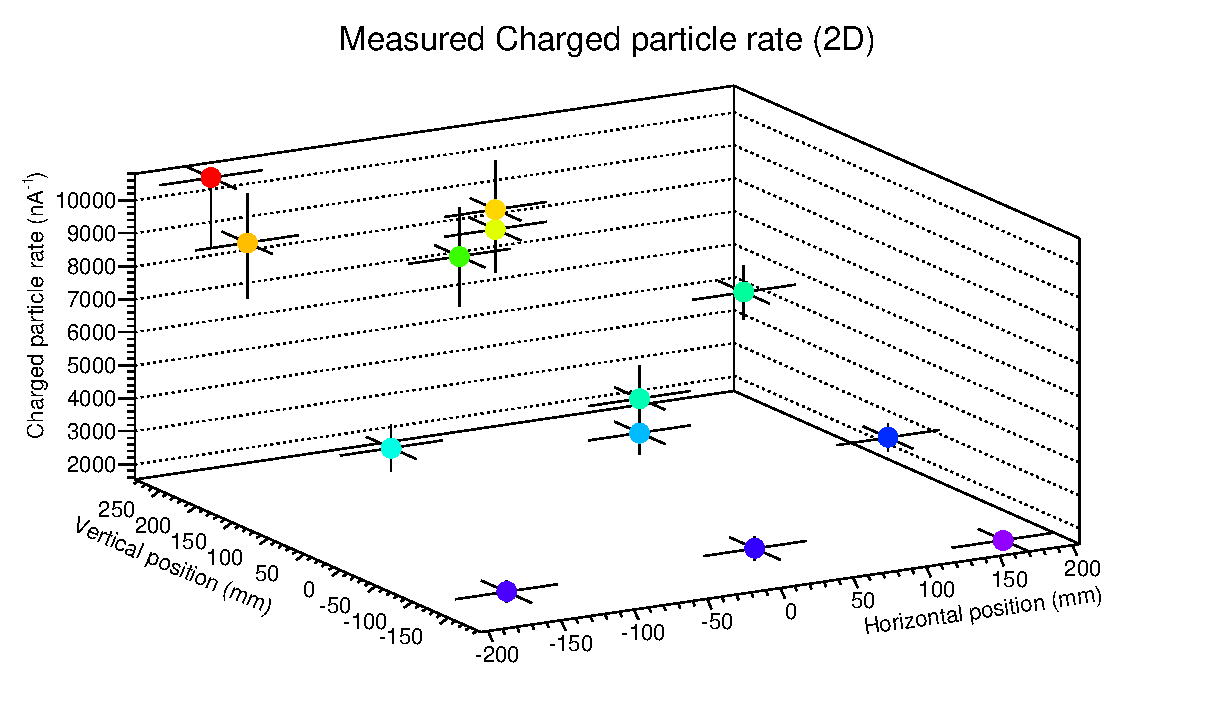
\includegraphics[width=.8\textwidth]{images/plot_generating_scripts/measured_2d_charged_flux.eps}
  \caption{2D plot of the charged particle flux across the front of the MuSIC beam pipe. The final three measurements were rescaled using the ratio of the two measurements at \((0,20)\)~cm.}
  \label{fig:2D_flux}
\end{figure}
 
% section results (end)
\subsection{Analysis} % (fold)
\label{sec:analysis}
As can be seen from the figures~\ref{fig:images_hit_rate_rescaled}~and~\ref{fig:2D_flux} the beam spot is positioned slightly up and to the left of the centre of the pipe. Where there were multiple measurements at the same position there is good agreement which suggests that the measurements are correct.

The agreement between the measurements and the simulation is less good as shown by figure~\ref{fig:images_plot_generating_scripts_1D_charged_particle_flux} where clearly the simulated rate and the measured rate are off by a significant amount (although both have the same shape). Comparing the simulation of the 2D case (figure~\ref{fig:sim_2d_charged_flux}) with the measurement (figure~\ref{fig:2D_flux}) we see that the simulation predicts a much more intense beam spot than what we see. This is likely due to the G4BL simulation having a much simpler model of the magnetic field at the position of the 2D measurement. The fluxes (with the exception of the peak at (0~cm, 20~cm)) are lower in the simulation than measured but not to the same degree as in the 1D case.

As figure~\ref{fig:sim_2d_charged_flux} shows both measurements agree on the general position of the beam spot. The measurements are not directly comparable due to the differences in both scintillator volume and position with respect to the end of the beam-pipe. Obviously the flux for the 2D measurement is generally lower due to smaller scintillator and greater distance from the beam-pipe.

The detector efficiency measurement for the 2D apparatus allows a more accurate calculation of the flux for this case whilst also providing a bench-mark efficiency for future uses of the scintillator/MPPC configuration (where it wasn't always possible to make an analogous measurement). 

The biggest problem, and one which was a cause of many issues, was the fragility of the MPPCs. Both the MPPC itself and the optical cement that bonded them to the scintillator were liable to break and this caused many problems that could not be easily fixed during the time available. 

A significant issue with the 1D measurement is the lack of a confirmation measurement that allows verification of the scaling factor applied to the later results. Even if the re-scaled points are ignored then they confirm that the beam spot is in the upper half of the pipe, a measurement later confirmed by the 2D measurement. 

Comparing the measured and simulated rates yields some interesting features. There is broad agreement on the general shape of the distribution but, using normalised plots, it appears that the measured charged particle rate for the 1D measurement is consistently higher than the simulated value by a factor of between 2 and 10. No obvious explanation of this presents itself as the measured value, should be, a lower bound whilst the simulated value should be closer to the `true' value due to lack of detector affects and similar. Whilst this suggests that further development of the G4BL simulation is required it is encouraging that MuSIC is performing above expectations, it also indicates that with improved experiments these sorts of measurements should provide useful data for tuning these models.

% \begin{figure}[hptb] 
%   \centering
%     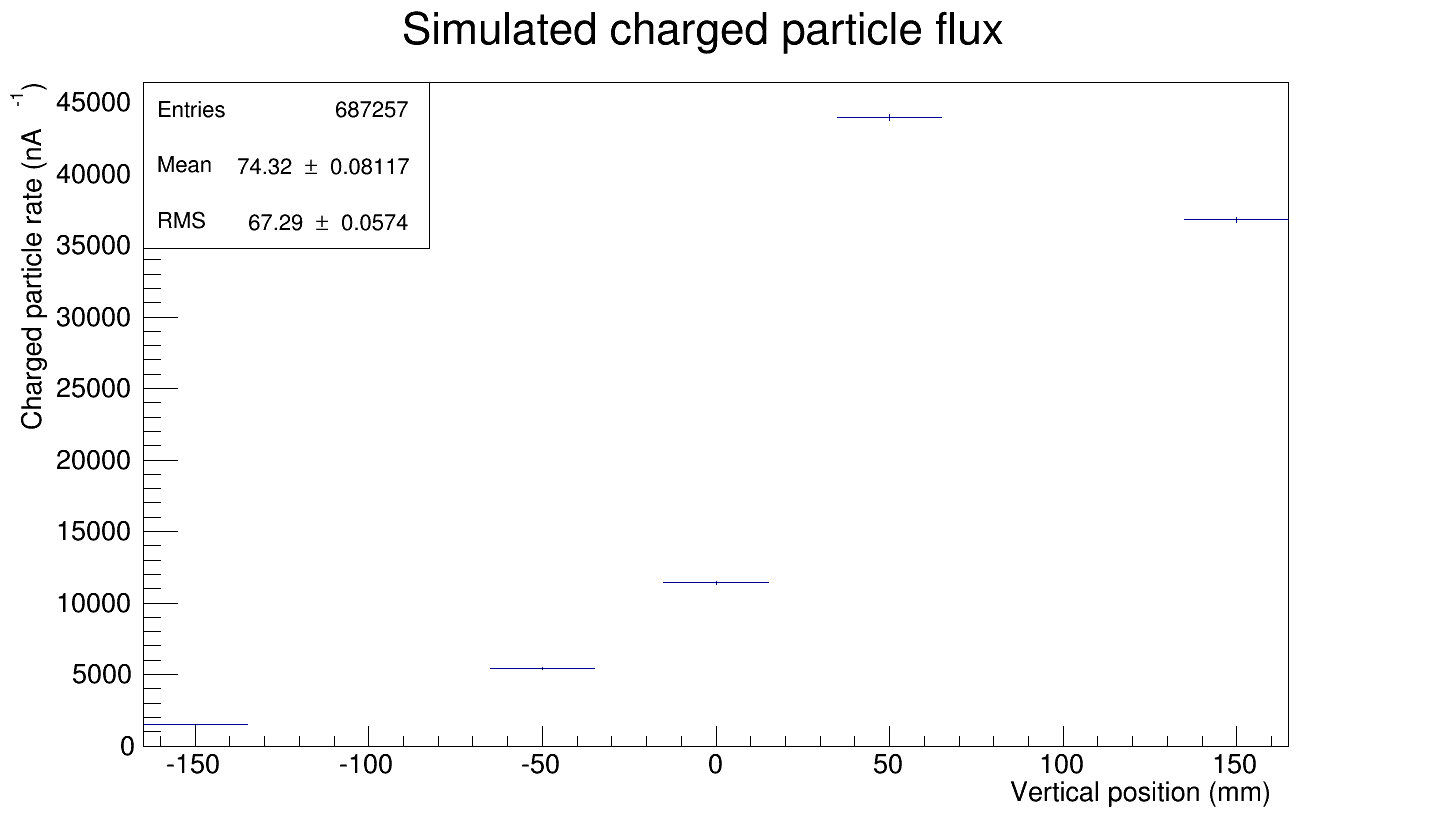
\includegraphics[width=.9\textwidth]{images/plot_generating_scripts/sim_1d_charged_flux.png}
%   \caption{Simulated results for the 1D charged particle rate, normalised to a proton current of 1~nA. Values calculated as the un-adjusted number of charged particles in the 1D scintillator volume from \( 9\times10^8 \) initial protons generated in G4BL.}
%   \label{fig:sim_1d_charged_flux}
% \end{figure}
\begin{figure}[hptb]
  \centering
    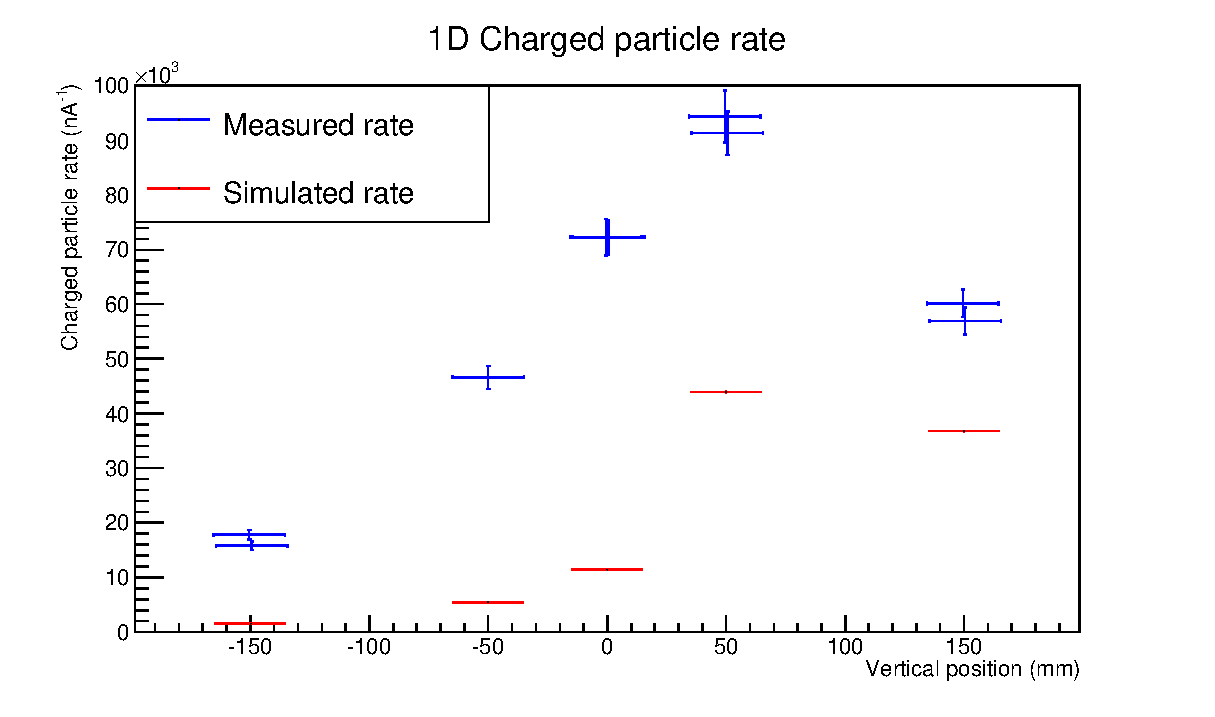
\includegraphics[width=.9\textwidth]{images/plot_generating_scripts/1D_charged_particle_flux.eps}
  \caption{Comparison of simulated and measured total charged particle flux.}
  \label{fig:images_plot_generating_scripts_1D_charged_particle_flux}
\end{figure}
  
\begin{figure}[hptb]
  \centering  
    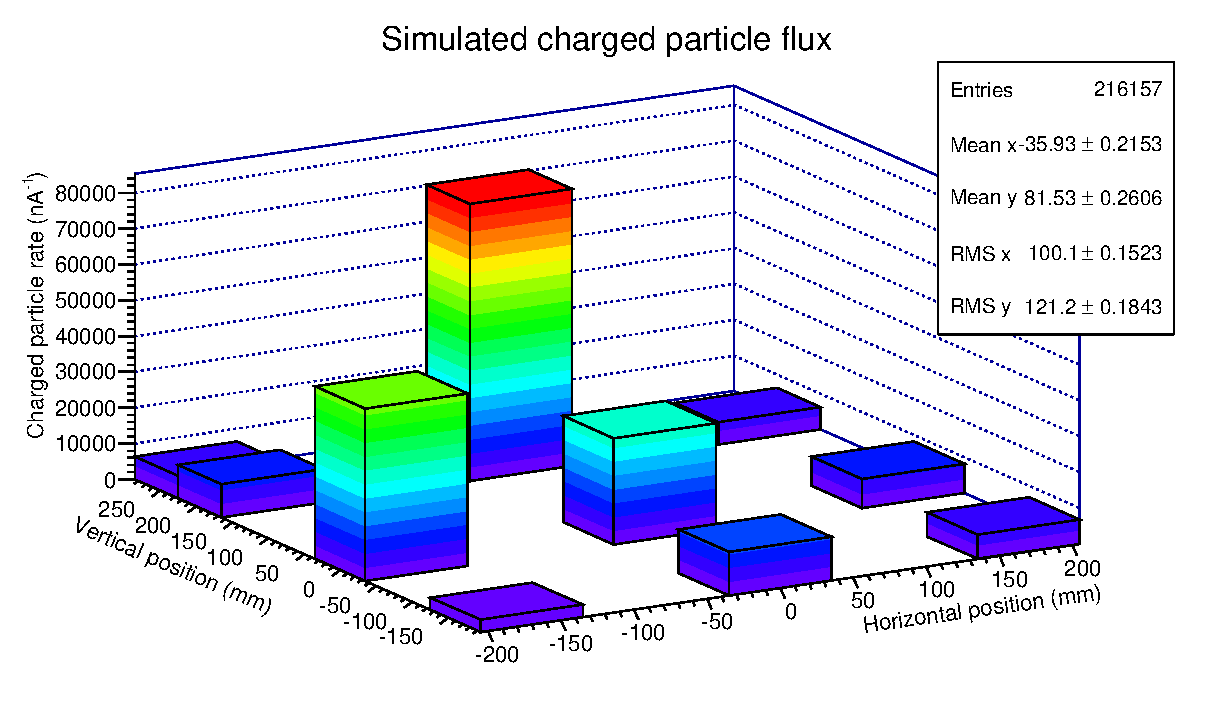
\includegraphics[width=.9\textwidth]{images/plot_generating_scripts/sim_2d_charged_flux.eps}
  \caption{Simulated results for the 2D charged particle rate normalised to a proton current of 1~nA. Colour is equal to the rate as given by the z-axis. Simulated using \( 9\times10^8 \) in G4BL, the rate was taken to be those particles seen within the area of the scintillator used.}
  \label{fig:sim_2d_charged_flux}
\end{figure}

% section analysis (end)
\clearpage
% chapter charged_particle_flux (end)

\section{Muon Lifetime} % (fold)
\label{cha:muon_lifetime}
Measurement of the muon lifetime was done to confirm the presence of muons in the beam. As has been discussed muons have a relatively long lifetime (\(2.197~\mu\)s) that is reasonably distinct from any others; this acts as a useful method of identification. To make the measurement two scintillators are placed on either side of a stopping target. The entire detector is placed perpendicular to the muon's direction of travel. The muons lose energy as they traverse the stopping target and some number of them will decay emitting an electron. By measuring the time differences between a detection at the upstream scintillator (the muon) and a detection at the downstream scintillator (the decay electron) we can spectrum the characteristic exponential decay and measure the muon lifetime. The curve produced is the sum of the many exponentials, each corresponding to the material in which negative muons were captured or the free decay of positive muons. As negative muons are less common at MuSIC than positive ones and because in many materials negative muons have similar lifetimes only two exponentials are typically used: one for the positive muons and another for negative muons captured by the stopping target which has a measurably different lifetime.

In total three measurements of the muon lifetime were taken: one concurrently with the 2D charged particle flux measurement, a high-statistics run and then measurements that form the basis of the muon momentum spectrum measurement. The first two of these measurements will be discussed here and the final one will be discussed later.

\subsection{Experimental Set Up} % (fold)
\label{sec:experimental_set_up}
The basic experimental set up for muon lifetime measurement has already been discussed: two scintillators sandwiching a stopping target. Both measurements were made using the same scintillator and stopping target: two \( 380\times50\times3.5 \)~mm\(^3\) scintillators and a \( 370\times80\times6 \)~mm\(^3\) pure copper target. An MPPC was mounted at either end of both scintillators (4 MPPCs in total) to provide read-out.

The DAQ used was a simple extension of the previous versions. This time, rather than measuring the time differences between the different individual MPPCs the TDC was used to measure the time between a hit on the upstream scintillator and then a hit on the downstream. A `hit' was considered to be a co-incident signal on both MPPCs of that scintillator. As a measure to reduce spurious signals due to other charged particles, e.g.\ electrons, a veto window of 50~ns was used. The veto window was a period following the upstream hit in which no hits were allowed in the downstream scintillator. The veto-window is used to reject particles that didn't decay between the scintillators or which decay but aren't muons (e.g.\ pions, which have a 26~ns lifetime).

% section experimental_set_up (end)
\subsection{Results} % (fold)
\label{sec:results} 
Figures~\ref{fig:music2_mu_lifetime} and \ref{fig:music3_muon_lifetime} show the TDC measurements that were made to record the muon lifetime. The TDC bin values are converted to ns using:
\begin{align}
  t = K(T - T_0)
\end{align}
where \(t\) is the real time, in ns, \(K\) is the calibration constant (0.025, measured by manufacturer), \(T\) is the value recorded in the MH-TDC and \(T_0\) is the time when the start signal for the TDC was sent, as recorded by the MH-TDC on a dedicated channel.

The data is then fitted with either one or two exponential decay functions and a flat background. Whether a single or double exponential is used depends heavily on the amount of data that was taken. A single function was used to fit the free decay of muons (neglecting the captured negative muons) whereas a second exponential was used to model the decay of captured negative muons inside the stopping target. Fitting the copper-decay exponential requires much more data as a significant proportion of the events from this are ignored because of the veto-window. In the first 50~ns \(\sim\)26~\% of all copper decays will have already occurred in comparison to only \(\sim\)2\% of free muon decays, this is made worse as the number of positive muons is significantly higher than the number of negative muons making the captured muon signal much lower.

\begin{figure}[hptb]
  \centering
  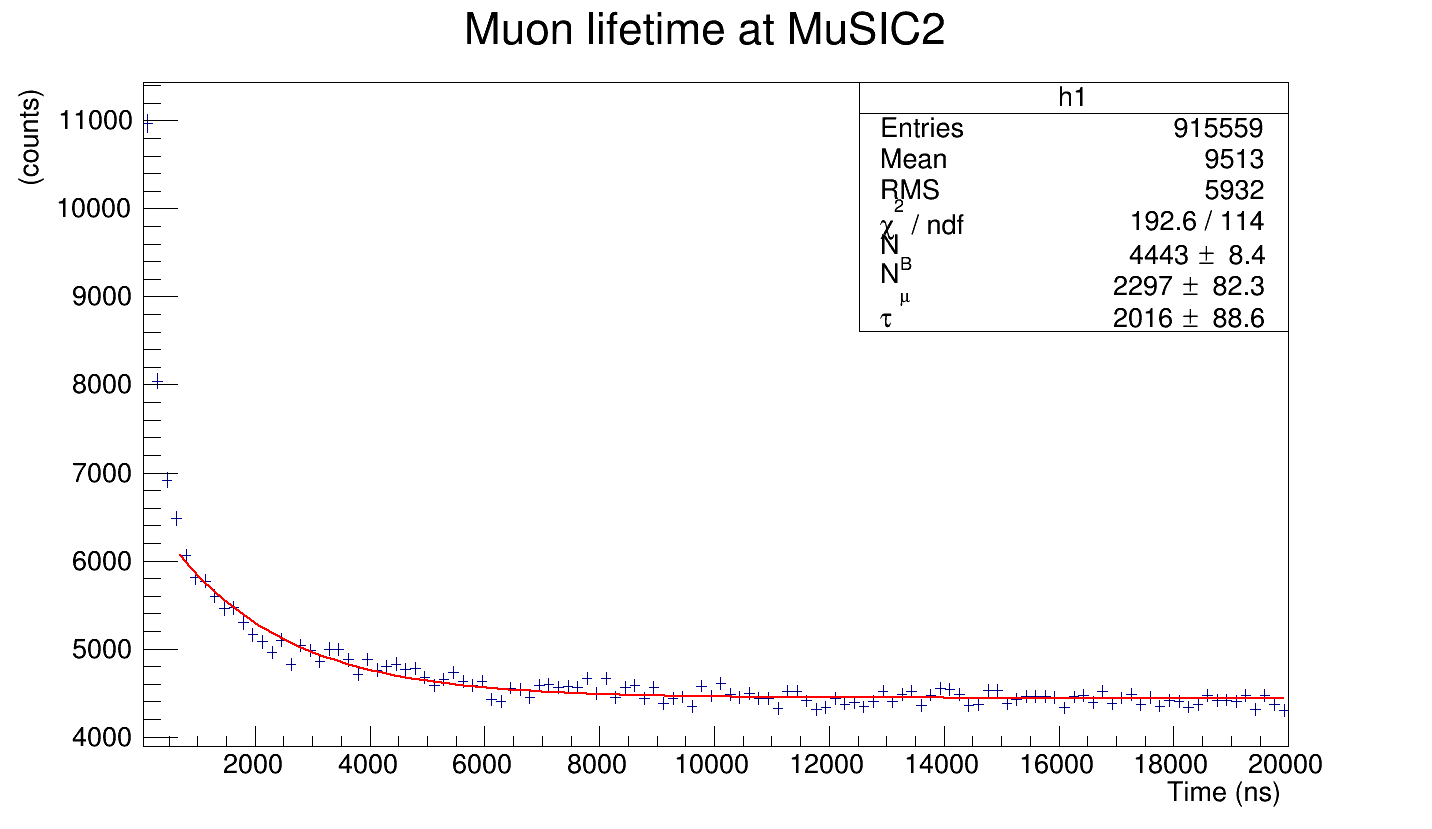
\includegraphics[width=.9\textwidth]{images/lifetime/music2_mu_lifetime_good.png}
  \caption{Results of the first measurement of the muon lifetime with residuals from the fit in the lower plot. The data was binned in 166~ns bins to remove the affects of noise on the data, only entries with an ADC value of 1,100 (which excluded the pedestal) were used. The fit was applied from 600~ns to 20~\(\mu\)s. The residuals show that fit gets worse at earlier times although this is to be expected with an exponential. Fitting with two exponentials should have improved the fit at earlier times but this was found not to be the case.}
  \label{fig:music2_mu_lifetime}
\end{figure}

% section results (end)
\subsection{Analysis} % (fold)
\label{sec:analysis}
As can be seen in figures~\ref{fig:music2_mu_lifetime} and \ref{fig:music3_muon_lifetime} the exponential decays are good fits to the data with reasonable chi-squared values (\(192.6/114\) and \( 516/231 \) respectively). The muon lifetimes measured are in reasonable agreement with the canonical value of \((2.1969811\pm0.0000022)\)~\(\mu\)s~\cite{pdg}. The lifetime measurement for the first run is low but this is to be expected as the fit doesn't account for the capture of negative muons which have a much shorter lifetime. Whilst both measurements have a large amount of background this does not remove from the core fact that large numbers of muons were detected and they exhibited the expected properties. The second measurement also produces a measurement of the muonic-copper lifetime which slightly higher than the \((163.5\pm1)\)~ns~\cite{suzuki_mu_capture_rates} measured by others but this discrepancy is small (\(<2\sigma\)) likely due to the presence of contaminating materials (e.g.\ the scintillator plastic).

\begin{figure}[hptb]
  \centering
  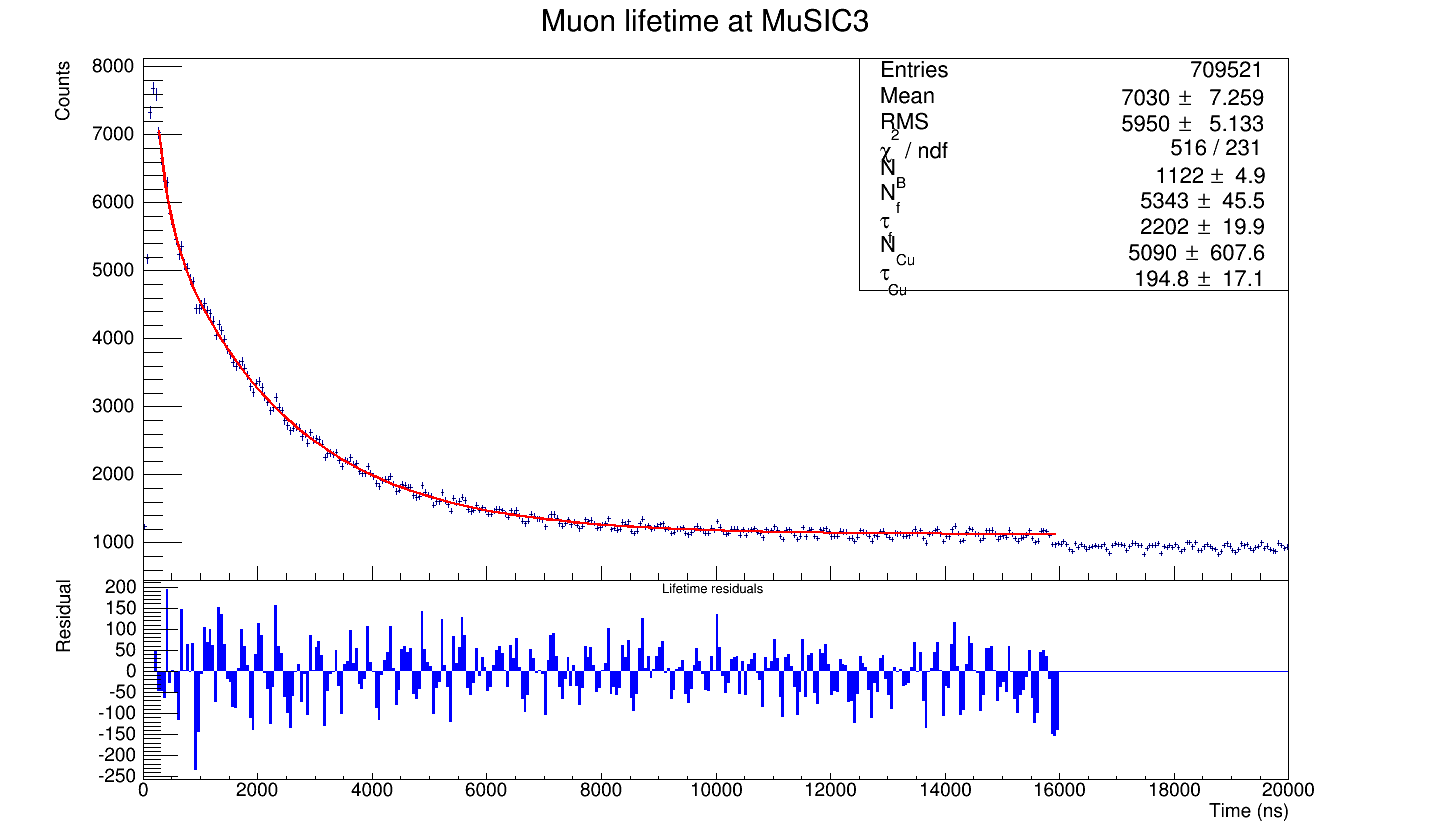
\includegraphics[width=.9\textwidth]{images/lifetime/music3_muon_lifetime.png}
  \caption{Results of the second measurement of the muon lifetime with residuals of the fit in the lower plot. The data was split between bins with a width of 50~ns and the data was fitted for values between 200~ns and 16~\(\mu\)s. The upper limit of the fit was lowered from the maximal 20~\(\mu\)s due to a fault that caused events to be missed at about 16~\(\mu\)s. The fault can be seen in the discontinuity at 16~\(\mu\)s, this is especially clear in the residuals (which have been extended beyond the fit to illustrate this point). The residuals also show a possibly periodic nature which is further explored in section~\ref{cha:momentum_spectrum}.}
  \label{fig:music3_muon_lifetime}
\end{figure}

% section analysis (end)

\clearpage
% chapter muon_lifetime (end)
\section{Momentum Spectrum} % (fold)
\label{cha:momentum_spectrum}
Measurement of the muon momentum spectrum was carried out using an extension of the muon lifetime measurement technique. The number of scintillators was increased to improve coverage of the beam-pipe. To make the momentum measurement, a range of degraders were used to select different (initial) ranges of muon momenta that would then stop. To determine the relation between degrader and stopped muon momentum the simulation was used.

% The final experiment carried out at MuSIC that we will discuss is the measurement of the muon momentum spectrum. The experiment was also extended so that rather than a single narrow scintillator several scintillators forming a basic hodoscope were employed giving coarse vertical flux information as well the desired momentum measurements.

\subsection{Experimental Set Up} % (fold)
\label{sec:experimental_set_up}
\subsubsection{Detector} % (fold)
\label{sub:detector}
The detector consisted of an aluminium degrader whose thickness could be varied to select different momentum ranges, a thin (0.5~mm) upstream counter and a thicker (3.5~mm) downstream counter on either side of a 0.5~mm copper stopping target, table~\ref{tab:detector_dimensions} gives details of the dimensions used. A schematic of the detector can be seen in figure~\ref{fig:m5_setup}. Based on simulation (see chapter~\ref{prt:simulation}) we predicted the mean initial momentum of muons that decay for different degrader thicknesses, the initial muon momentum distribution is given in figure~\ref{fig:images_momentum_spectrum_muon_momentum_at_beam_pipe_exit} and the momentum distributions for the muons that stop in the detector can be seen in figure~\ref{fig:images_momentum_spectrum_stopped_muon_momentum}, the mean momentums are also tabulated in table~\ref{tab:stopped_muon_mom}.
\begin{table}
  \begin{center}
  \begin{tabular}{l | c | c | c | c | c}
    \multirow{2}{*}{Component}  &  \multirow{2}{*}{Material}  
                                            &  \multicolumn{3}{c|}{Dimensions (mm)}  &  \multirow{2}{*}{Number} \\
                                &           &      X      &      Y     &       Z     &                          \\
    \hline
    Degrader                    &    Al     &     400     &     400    &  0.5, 1, 5  &  1                       \\
    Upstream scintillator       &  EJ-212   &     380     &     30     &      0.5    &  8                       \\    
    Stopping Target             &    Cu     &     370     &     310    &      0.5    &  1                       \\    
    Downstream scintillator     &  EJ-212   &     380     &     50     &      3.5    &  5                       \\    
  \end{tabular}
  \end{center}
  \caption{Dimensions of the various detector components. The `Z' is the beam direction, `Y' is vertical and `X' is horizontal. The layout of the detector can be seen in figure~\ref{fig:m5_setup}.}
  \label{tab:detector_dimensions}
\end{table}

\begin{figure}[htbp]
    \centering
        \includegraphics[scale=0.5]{images/momentum_spectrum/Detector_setup_music5.png}
    \caption{Experimental set up of the detector for MuSIC~5 (widths not to scale), see table~\ref{tab:detector_dimensions} for actual sizes. The upstream scintillators are outlined with blue dashes whilst the downstream ones are red dots.}
    \label{fig:m5_setup}
\end{figure}  

\begin{figure}[hptb]
  \centering
    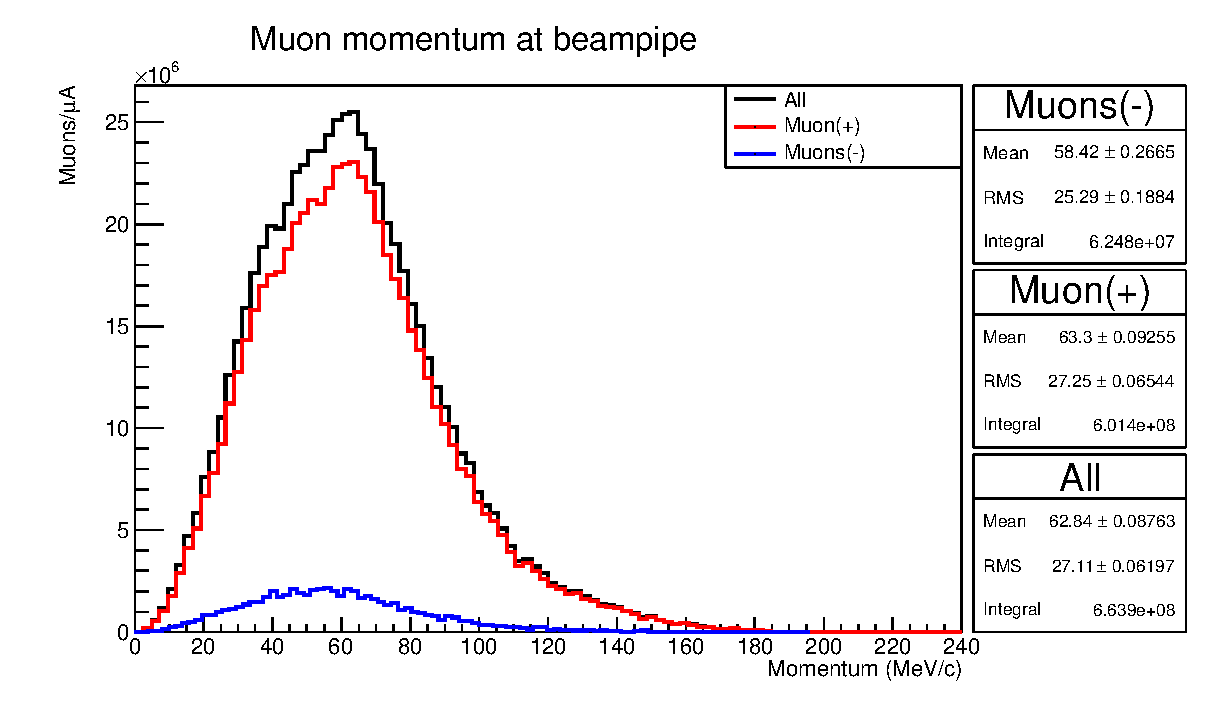
\includegraphics[width=.9\textwidth]{images/momentum_spectrum/muon_momentum_at_beam_pipe_exit.eps}
  \caption{Total muon momenta at the end of the beam pipe. The number of initial muons simulated was 95,700. The plot has been normalised to the number of muons per \(\mu\)A of proton beam.}
  \label{fig:images_momentum_spectrum_muon_momentum_at_beam_pipe_exit}
\end{figure}

\begin{figure}[hptb]
  \centering
    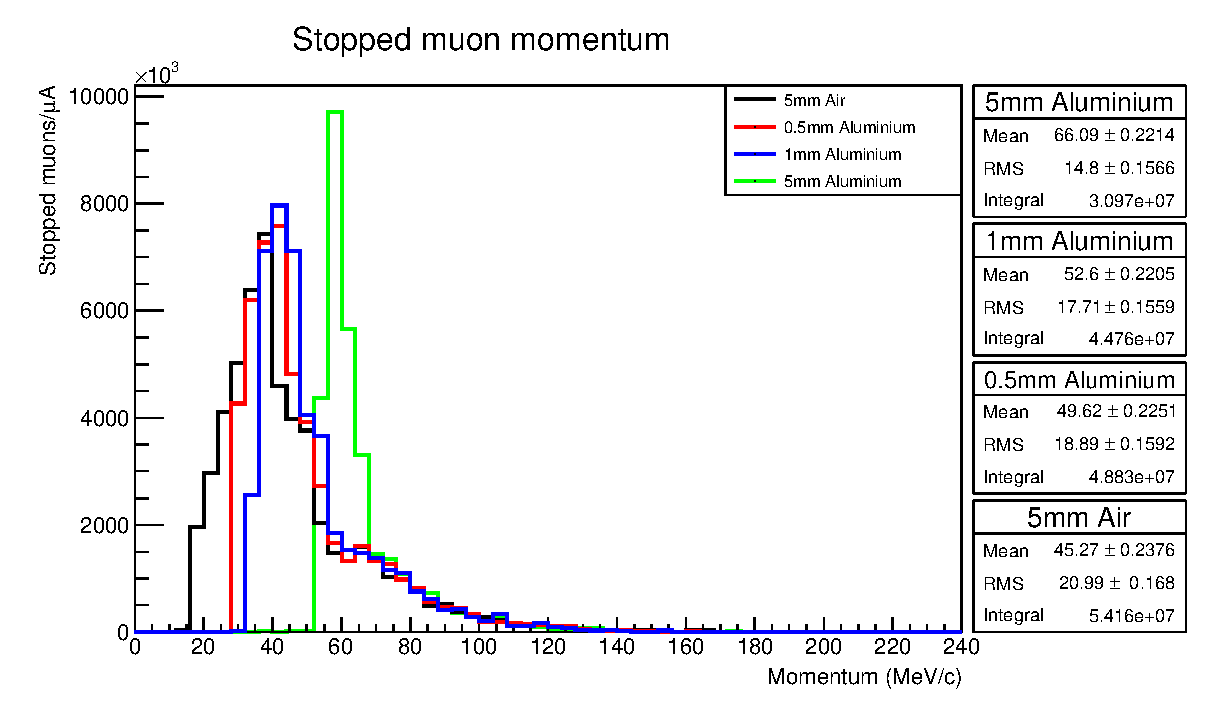
\includegraphics[width=.8\textwidth]{images/momentum_spectrum/stopped_muon_momentum.eps}
  \caption{Momenta at the end of the beam pipe of muons that subsequently stopped. This shows the momenta that the different degraders `select'. The number of initial muons simulated was 95,700. The plot has been normalised to the number of muons per \(\mu\)A of proton beam.}
  \label{fig:images_momentum_spectrum_stopped_muon_momentum}
\end{figure}

\begin{table}
  \lineup
  \begin{center}
  \begin{tabular}{c | r@{\(\pm\)}l | r@{\(\pm\)}l }
    Degrader  &  \multicolumn{4}{c}{Momentum (MeV/c)}      \\
      (mm)    &  \multicolumn{2}{c|}{Mean}  
                               &  \multicolumn{2}{c}{RMS}  \\
    \hline
      0.0     &  45.27 & 0.24  &  20.99 & 0.17             \\
      0.5     &  49.62 & 0.23  &  18.89 & 0.16             \\
      1.0     &  52.60 & 0.22  &  17.71 & 0.16             \\
      5.0     &  66.09 & 0.22  &  14.80 & 0.16             \\
  \end{tabular}
  \end{center}
  \caption{Simulated mean and Root Mean Squared (RMS) momenta of muons, that subsequently stop, at the end of the beam pipe. The degrader is the thickness of the aluminium, the width and height are both 400~mm. The Geant4 simulation was used; in total 95,700 initial muons were simulated, for further details see chapter~\ref{prt:simulation}.}
  \label{tab:stopped_muon_mom}
\end{table}

The counters used were mylar wrapped scintillators with read-out performed by MPPCs mounted on either end of a wavelength shifting fibre bounded along the long axis of the scintillator using optical cement. The signals from each pair of MPPCs are combined and amplified before being passed to the data acquisition system (DAQ) for processing.

Two important considerations were made with the choice of scintillators: the upstream scintillator had to minimise perturbation of the beam whilst providing a suitable trigger from muons and the downstream scintillator had to be effective at detecting electrons. To this end a thin (0.5~mm) upstream scintillator and thicker (3.5~mm) downstream scintillator were chosen. One downside of this set up is that in using a thin upstream scintillator the efficiency for detecting minimally ionising particles is reduced but as only stopping muons were desired this has a negligible effect.

\subsubsection{Data Acquisition} % (fold)
\label{sub:data_acquisition}
The DAQ system used was a simple evolution of that used in the previous experiments: a discriminator unit with paired logic block formed a trigger on a suitably strong upstream signal with no downstream signal within a 50~ns veto window. The triggering signal was recorded using QDC (although it is not analysed here) and a MH-TDC was used to record hit times at all scintillators \(\pm\)20~\(\mu\)s of the trigger. To increase the accuracy of the MH-TDC the trigger time is recorded on a separate channel to the individual MPPC signals called `TDC0' which can then be removed later.

For a signal to be recorded or used as a trigger the discriminator was set to exclude events with fewer than eight photons in the upstream scintillator and fewer than ten in the downstream. The reason for these high values is that each analogue signal, as passed to the discriminator, is the combination of the signals from both the MPPCs on a scintillator. The thinner upstream scintillator has a lower threshold as it's aimed at selecting slow muons that will stop, unfortunately this means it cannot detect mips but these are unlikely to stop. Conversely the downstream scintillator has been set up to select electrons which will deposit more energy and the higher threshold will help reduce background.

A scaler was used to record system diagnostics through regular polling. The values recorded were:
\begin{enumerate}
  \item SEC output.
  \item Triggers (i.e.\ \textsc{u and }\(\overline{\textsc{d}}\)\textsc{ and }\(\overline{\textsc{busy}}\)\footnote{Where `\textsc{u}' is a suitable upstream signal, `\textsc{d}' is a signal in the downstream scintillator and `\textsc{busy}' indicates that the system is busy. Barred values indicate negation, i.e.\ \(\overline{\textsc{d}}\) indicates no downstream signal and \(\overline{\textsc{busy}}\) indicates that the system isn't busy.}).
  \item Potential triggers (i.e.\ \textsc{u and }\(\overline{\textsc{d}}\)).
  \item A clock (for accurate run measurement).
\end{enumerate}
Obviously the clock and SEC were used for normalisation whilst the triggers and potential triggers were used for calculation of dead time (see section~\ref{sub:dead_time}).

% subsection data_acquisition (end)
% section experimental_set_up (end)
\subsection{Data Processing} % (fold)
\label{sec:data_processing}
There were five stages in preparing the data for analysis: reading from VME, calibration and binning. At the end of these processes the data was analysed and the final measurements made. Six data sets were chosen for this analysis, the run conditions are listed in table~\ref{tab:run_summary}.

\begin{table}
	\begin{center}
	\begin{tabular}{c|c|c|c}
		Run ID & Time (sec) & Current (pA) & Degrader (mm) \\
		\hline
		448    & 9,221      & 15           & 0.0   \\
		451    & 1,001      & 15           & 0.5   \\
		452    & 4,924      & 13           & 0.5   \\
		455    & 6,307      & 13           & 1.0   \\
		458    & 5,144      & 14           & 5.0   \\
		459    & 2,452      & 12           & 5.0   \\
	\end{tabular}
	\end{center}
	\caption{Summary of the runs selected for this analysis. The degrader used aluminium and the stopping target 0.5~mm copper.}
	\label{tab:run_summary}
\end{table} 

The data was read from VME using the MIDAS program (`a general purpose data acquisition system for small and medium scale experiments'~\cite{midas_daq}), this dealt with the low level interface to CAMAC and allowed basic plotting of the information.

Once the data was saved, it was calibrated to convert it to convert it to real world measurements. The calibration formula for the MH-TDC was:
\begin{align}\label{equ:tdc_calibration}
    t'   &= 0.024414(t - \text{TDC0})
\end{align}
where \(t'\) is the calibrated time, \(t\) is the MH-TDC value and TDC0 is the time at which the trigger occurred. The calibration co-efficient of \(0.024414\) was determined using a known clock as input to the MH-TDC and then detecting a set number of ticks that could then be read off as MH-TDC values.

The final stage of data preparation was to bin the data, this was done to make later analysis quicker. Each channel had its MH-TDC times combined in 1~ns bins. This left suitable accuracy whilst vastly reducing the data set's size.

\subsection{Secondary calculations} % (fold)
\label{sec:secondary_calculations}
Using the scaler information two checks could be made: the dead time and the Periodic Trigger Rate (PTR). The dead time of the system is a measure of how many events are lost because the system is busy. The PTR is a check that the rate of triggering events is reasonably constant, deviations from a constant rate would indicate possible problems with the data.

\subsubsection{Dead time} % (fold)
\label{sub:dead_time}
As was stated in section~\ref{sub:data_acquisition} the scaler was used to record diagnostics on the DAQ. To calculate the dead time, the trigger count and the potential trigger count are needed which can be used thus:
\begin{align}
    \text{Live time} &= \frac{\text{Good Triggers}}{\text{Potential Triggers}} \\
    \text{Dead time} &= 1 - \text{Live Time} \\
\end{align}
Where potential triggers are those with a signal in the upstream scintillator and no corresponding signal downstream within the 50~ns veto window. A good trigger is a potential trigger that occurs without the system being busy. The results of this calculation are given in table~\ref{tab:dead_time}.
\begin{table}
    \begin{center}
    \begin{tabular}{c | c | c | r@{ $\pm$ }l | r@{ $\pm$ }l | r@{ $\pm$ }l | r@{ $\pm$ }l }
        \multirow{2}{*}{Run} 
             &  Degrader  &  Length 
                              & \multicolumn{4}{c|}{Triggers (\(\times10^3\))}
                              & \multicolumn{2}{c|}{Live time}
                              & \multicolumn{2}{c}{Dead time}  \\
             & (mm)       & (s)               
                              & \multicolumn{2}{c|}{Good}
                              & \multicolumn{2}{c|}{Potential}
                              & \multicolumn{2}{c|}{(\%)}
                              & \multicolumn{2}{c}{(\%)}  \\
        \hline
        448  &  0.0  &  9221  &  9653.0 & 3.1   &  15678.8 & 4.0  &  61.57 & 0.03  &  38.43 & 0.025 \\
        451  &  0.5  &  1001  &  767.32 & 0.88  &   1070.4 & 1.0  &  71.69 & 0.11  &  28.31 & 0.107 \\
        452  &  0.5  &  4944  &  3459.9 & 1.9   &   4667.8 & 2.2  &  74.12 & 0.05  &  25.88 & 0.053 \\
        455  &  1.0  &  6307  &  4090.2 & 2.0   &   5372.4 & 2.3  &  76.13 & 0.05  &  23.87 & 0.050 \\
        458  &  5.0  &  5144  &  2049.1 & 1.4   &   2455.0 & 1.6  &  83.47 & 0.08  &  16.53 & 0.079 \\
        459  &  5.0  &  2452  &  915.31 & 0.96  &   1077.5 & 1.0  &  84.95 & 0.12  &  15.05 & 0.121 \\
    \end{tabular}
    \end{center}
    \caption{Dead and live times for each run along with the number of potential and good triggers. Run time is included to show the origin of the different counts.}
    \label{tab:dead_time}
\end{table}
% subsection dead_time (end)
\subsubsection{Trigger Rate} % (fold)
\label{sub:gain_stability}
To ensure that there were no problems during data taking the trigger rate was checked. The trigger rate gives a measure of how consistent the detector was as well as highlighting any possible problems in the run. Each run was split into 100 equal sections and the trigger rate determined using the values recorded by the scaler. The results are plotted in figure~\ref{fig:gain_stability} and fitted with a flat function. As can be seen as the degrader's thickness increases the trigger rate goes down. There are also some peaks in the first run (448), it is unclear what caused this. The SEC data (also plotted) does not suggest that the fluctuations in the rate are due to changes in the beam. This effect is a source of systematic errors but these are small compared to those due to the detector efficiency.
%
\begin{sidewaysfigure}
  % \begin{figure}%[htbp]
      \centering
          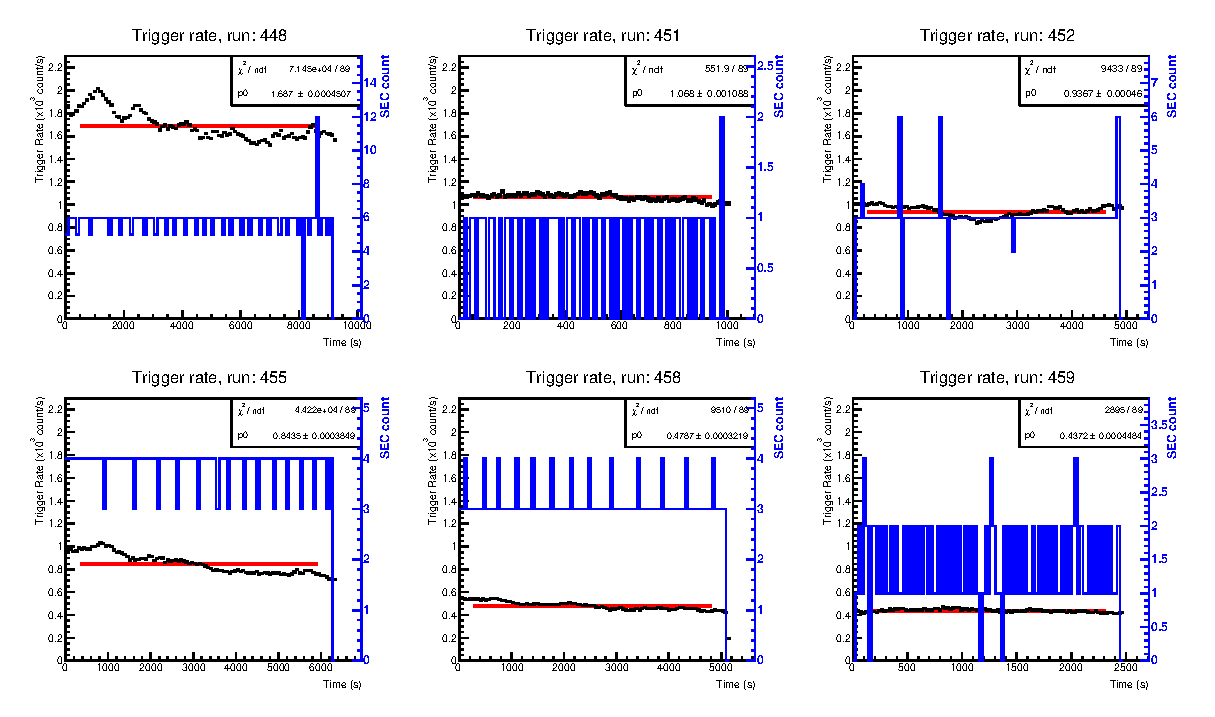
\includegraphics[width=\textwidth]{images/momentum_spectrum/gain_stability.eps}
      % \caption{Trigger rate of each run, split over 100 measurements. The triggers used were potential and so exclude any rate limiting due to dead time. The central 90~\% of the data has been fitted with an order 0 polynomial with the parameters given.}
      \caption{Trigger rate of each run (black) with the raw SEC count (blue). 100 samples were taken from the scaler data. Potential triggers were used to exclude any rate limiting due to dead time. The central 90~\% of the data has been fitted with an order 0 polynomial with the parameters given. The SEC values are the differences of the count at the start of the time window and the end, this was done because the SEC value was not reset between measurements within a run. The SEC data suggests that the fluctuations in the trigger rate are not due to changes in the beam.}
      \label{fig:gain_stability}
  % \end{figure}
\end{sidewaysfigure}

% %
% \begin{table}
%     \begin{center}
%         \begin{threeparttable}
%             \begin{tabular}{c|c|c|c|r@{ $\pm$ }l}
%                 Run & Al degrader thickness (mm) & $\chi^2$ 
%                                                  & N.D.F. \tnote{a}
%                                                  & \multicolumn{2}{|c}{Gain} \\
%                 \hline
%                 448  &  0.0  &  52.94   &  9  &  1.682  &  0.015  \\
%                 451  &  0.5  &  0.8361  &  9  &  1.065  &  0.029  \\
%                 452  &  0.5  &  14.7    &  9  &  0.940  &  0.011  \\
%                 455  &  1.0  &  83.68   &  9  &  0.8331 &  0.0089 \\
%                 458  &  5.0  &  83.41   &  9  &  0.4634 &  0.0055 \\
%                 459  &  5.0  &  1.964   &  9  &  0.4363 &  0.0075 \\
%             \end{tabular}
%             \caption{Gains as determined by the fits to the gain stability in figure~\ref{fig:gain_stability}.}
%             \begin{tablenotes}
%                 \item [a] Number of Degrees of Freedom
%             \end{tablenotes}
%             \label{tab:gain_stability_paramters}
%         \end{threeparttable}
%     \end{center}
% \end{table}

% subsection gain_stability (end)
% section secondary_calculations (end)
\subsection{Results} % (fold)
\label{sec:momenta_results}
As has been discussed there are six data sets that were used for this analysis, the details of them are given in table~\ref{tab:run_summary}. For this analysis only the downstream scintillators are used to calculate the decay times as this was the scintillator best configured to detect them whilst the upstream scintillator was used to form the trigger. Each run was analysed in the same way, once processing was complete (section~\ref{sec:data_processing}) the binned data was converted into a histogram and fitted using:
\begin{align}
  N_{f}\exp\left(\frac{-t}{\tau_{f}}\right) + N_{c}\exp\left(\frac{-t}{\tau_{c}}\right) + N_{s}\sin\left(2\pi\frac{t-\phi}{T}\right) + N_{b} \label{equ:fit}
\end{align}
\(t\) is the time in ns. The four terms each have their own subscript based on what they describe: free muon decay (\(f\)); decay of negative muons captured by the stopping target (\(c\)); a sinusoidal background (\(s\)) and a flat background (\(b\)). The two muon decay terms are parameterised with a scale factor (\(N\)) and a lifetime (\(\tau\)). The sinusoidal term has a period (\(T\)) and phase, relative to the trigger time, (\(\phi\)). 

Originally only a flat background was used but this was found to be insufficient to describe the data and the sinusoidal component was introduced. The sinusoidal effect is thought to be minor bunching of the protons due to the AVF acceleration system which has a stated frequency of 6--18~MHz~\cite{avf_facility} (or a period of 167--56~ns respectively). The flat background is made by travelling particles that don't form a trigger but are recorded by the MH-TDC.

In order to have good statistics whilst maintaining sensitivity to the relatively fast copper component of the decays a bin width of 16~ns was used. A large bin width (e.g.\ 100~ns) could have been used to smooth the sinusoidal noise but this would result in very few bins in which the copper component was significant. Whilst the ideal solution would be to use binning such that the sinusoidal component was cancelled out this was not feasible due to limitations of the fitting program. In the end a bin width was chosen that resulted in a small \(\chi^2\) whilst remaining sensitive to copper.

Fitting all the parameters could not easily be done freely due to the range of values to which it was being fitted; some features (e.g.\ the periodic noise) had a scale of \(\mathcal{O}\)(60)~ns compared to the free decay \(\mathcal{O}\)(2,000)~ns and the entire fit range \(\mathcal{O}\)(20,000)~ns. To mitigate the problem of scale the known values, \(\tau_{f}\) and \(\tau_{c}\), were fixed at their given values of \(2,196.9811\pm0.0022 \)~ns~\cite{pdg} and \( 163.5\pm1 \)~ns~\cite{suzuki_mu_capture_rates} respectively. The period, \(T\), was constrained to \(60\pm5\)~ns which was determined to be a good value from fitting the noise in isolation (see figure~\ref{fig:images_momentum_spectrum_448_D1_noise_fit}).

\begin{figure}[hptb]
  \centering
    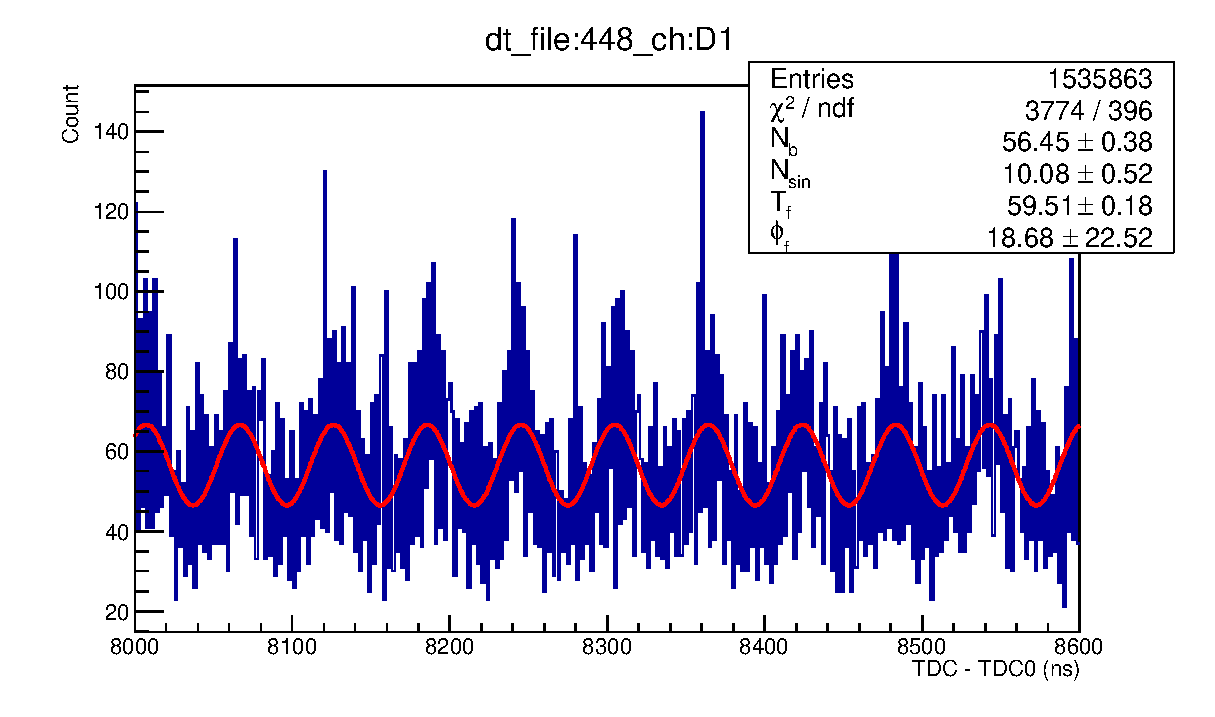
\includegraphics[width=.9\textwidth]{images/momentum_spectrum/448_D1_noise_fit.eps}
  \caption{Zoomed region (8,000~to~8,600~ns) of run 448, channel D1, showing the sinusoidal component of the background, the background has been fitted using \(N_b + N_s\sin(2\pi\frac{t-\phi}{T})\).}
  \label{fig:images_momentum_spectrum_448_D1_noise_fit}
\end{figure}

Once the data was fitted the \(f\) and \(c\) terms were integrated individually to calculate the number of free and copper decays the muons underwent. The fitted histograms are shown in figures~\ref{fig:images_momentum_spectrum_448}~to~\ref{fig:images_momentum_spectrum_459} and the results are summarised in table~\ref{tab:fit_res}. The fitting shows that the bottom channels (D4 and D5) have the worst fit results, often chi-squared values of \(>10,000 / 1,239\)~(ndf), this is compared to values of \(\mathcal{O}(2,000) / 1,239\) for the other channels. Of the other channels D1 and D3 are generally best but D2 is consistently good enough to be useable (unlike channels D4 and D5 which are removed from later analysis).

\begin{table}[hptb]
  \lineup % enable \0, \- & \.
  \begin{center}
  \begin{tabular}{ c | c | r@{\(\,\pm\,\)}l | r@{\(\,\pm\,\)}l | r@{\(\,\pm\,\)}l | r@{\(\,\pm\,\)}l | r@{\(\,\pm\,\)}l }
  % \begin{tabular}{ c | c | S@{\(\pm\)}S | S@{\(\pm\)}S | S@{\(\pm\)}S | S@{\(\pm\)}S | S@{\(\pm\)}S }
    Run  
      &  Ch.  
             & \multicolumn{2}{c|}{\(N_b\)} 
                                 &  \multicolumn{2}{c|}{\(N_s\)}
                                                     &  \multicolumn{2}{c|}{\(\phi\)}  
                                                                         & \multicolumn{2}{c|}{\( N_c \)}
                                                                                           &\multicolumn{2}{c}{\( N_f \)} \\
    \hline
    \multirow{5}{*}{448}
      &  D1  &  576.85\0& 0.80   &  121.10\0& 1.15   &   2.19 & 0.21    &   549\.\0& 31    &  1377.2\0& 5.7  \\
      &  D2  &  914.39\0& 1.0    &  197.28\0& 1.44   &  10.33 & 0.16    &  1524\.\0& 38    &  1937.2\0& 6.9  \\
      &  D3  &  164.22\0& 0.43   &   40.68\0& 0.63   &  18.22 & 0.36    &   592\.\0& 21    &   620.3\0& 3.4  \\
      &  D4  &   32.07\0& 0.19   &    6.89\0& 0.28   &  57.02 & 0.96    &   193\.\0& 11    &   172.8\0& 1.7  \\
      &  D5  &   27.79\0& 0.18   &    6.37\0& 0.26   &   4.31 & 0.94    &    24.8  &\07.8  &    91.1\0& 1.4  \\
    \hline
    \multirow{5}{*}{451}
      &  D1  &   39.55\0& 0.21   &    2.38\0& 0.31   &  25.3\0& 2.4     &    29.4  &\08.1  &   101.4\0& 1.5   \\
      &  D2  &   62.27\0& 0.26   &   17.74\0& 0.38   &  13.28 & 0.50    &   153\.\0& 11    &   178.2\0& 1.9   \\
      &  D3  &   11.52\0& 0.12   &    3.60\0& 0.17   &  20.4\0& 1.2     &    85.6  &\06.5  &    57.76 & 0.99  \\
      &  D4  &    2.18\0& 0.05   &    0.61\0& 0.08   &   6.5\0& 3.0     &    25.9  &\03.5  &    16.59 & 0.49  \\
      &  D5  &    1.97\0& 0.05   &    0.65\0& 0.07   &   8.7\0& 2.6     &     7.3  &\02.6  &     8.78 & 0.40  \\
    \hline
    \multirow{5}{*}{452}
      &  D1  &  161.25\0& 0.43   &   43.56\0& 0.61   &   4.08 & 0.31    &   208\.\0& 17    &   435.5\0& 3.1  \\
      &  D2  &  252.14\0& 0.54   &   71.73\0& 0.76   &  12.39 & 0.25    &   706\.\0& 23    &   789.9\0& 4.0  \\
      &  D3  &   46.29\0& 0.23   &   15.70\0& 0.34   &  19.82 & 0.55    &   335\.\0& 13    &   266.7\0& 2.1  \\
      &  D4  &    8.95\0& 0.11   &    2.49\0& 0.16   &   0.00 & 1.64    &   128.2  &\07.5  &    76.6\0& 1.1  \\
      &  D5  &    8.01\0& 0.097  &    2.37\0& 0.14   &   7.54 & 1.43    &    25.9  &\05.2  &    38.71 & 0.82  \\
    \hline
    \multirow{5}{*}{455}
      &  D1  &  187.67\0& 0.46   &   46.99\0& 0.66   &   4.38 & 0.32    &   265\.\0& 19    &   539.1\0& 3.4  \\
      &  D2  &  293.99\0& 0.58   &   73.76\0& 0.83   &  12.41 & 0.26    &   896\.\0& 26    &   967.9\0& 4.4  \\
      &  D3  &   54.02\0& 0.25   &   17.18\0& 0.37   &  20.27 & 0.53    &   438\.\0& 15    &   326.4\0& 2.3  \\
      &  D4  &   10.37\0& 0.11   &    2.86\0& 0.16   &   0.00 & 0.36    &   195.1  &\08.5  &    87.4\0& 1.1  \\
      &  D5  &    9.30\0& 0.10   &    2.63\0& 0.15   &   4.8\0& 1.3     &    41.9  &\05.8  &    47.00 & 0.90  \\
    \hline
    \multirow{5}{*}{458}
      &  D1  &   73.73\0& 0.29   &   21.53\0& 0.43   &   0.000 & 0.037  &   219\.\0& 15    &   350.2\0& 2.4  \\
      &  D2  &  114.37\0& 0.37   &   34.08\0& 0.54   &   5.32\0& 0.38   &   799\.\0& 20    &   562.4\0& 3.1  \\
      &  D3  &   21.47\0& 0.16   &    8.40\0& 0.24   &   9.89\0& 0.71   &   236\.\0& 11    &   178.1\0& 1.6  \\
      &  D4  &    3.805 & 0.070  &    1.25\0& 0.10   &   0.00\0& 0.19   &    72.6  &\05.8  &    49.23 & 0.80  \\
      &  D5  &    3.728 & 0.067  &    1.436 & 0.098  &   0.00\0& 0.76   &    19.1  &\04.2  &    28.11 & 0.65  \\
    \hline
    \multirow{5}{*}{459}
      &  D1  &   30.67\0& 0.19   &    8.86\0& 0.28   &  56.68 & 0.72    &   115.3  &\09.8  &   155.0\0& 1.6  \\
      &  D2  &   48.07\0& 0.24   &   14.91\0& 0.35   &   4.36 & 0.56    &   369\.\0& 13    &   254.0\0& 2.1  \\
      &  D3  &    8.87\0& 0.11   &    3.65\0& 0.16   &  11.3\0& 1.0     &   110.1  &\07.3  &    81.0\0& 1.1  \\
      &  D4  &    1.631 & 0.046  &    0.579 & 0.068  &  48.2\0& 3.1     &    39.2  &\04.9  &    22.01 & 0.54  \\
      &  D5  &    1.496 & 0.043  &    0.615 & 0.063  &   0.0\0& 1.0     &     8.0  &\02.8  &    12.73 & 0.43  \\
  \end{tabular}
  \end{center}
  \caption{Summary of the fitted values for equation~\eqref{equ:fit}. These are the values used for the calculation of the integrals and, ultimately, the muon rates. The two lifetime parameters, \( \tau_f \) and \( \tau_c \), were fixed at the values \(2,196.9811\pm0.0022 \)~ns~\cite{pdg} and \( 163.5\pm1 \)~ns~\cite{suzuki_mu_capture_rates} respectively, \( T \) was fixed at 60~ns.}
  \label{tab:fit_res}
\end{table}

\begin{sidewaysfigure}
    \centering
      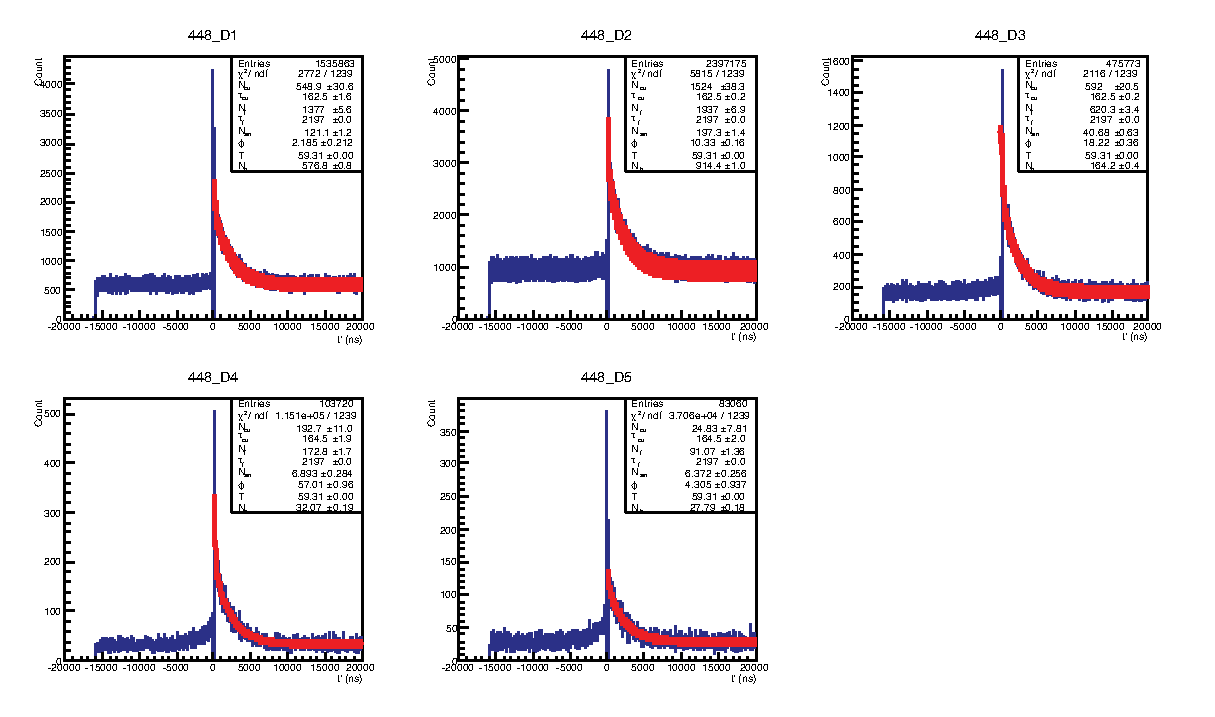
\includegraphics[scale=1]{images/momentum_spectrum/448.eps}
    \caption{Per channel fitting of data for run 448, for this run there was no degrader.}
    \label{fig:images_momentum_spectrum_448}
\end{sidewaysfigure}
%
\begin{sidewaysfigure}
    \centering
      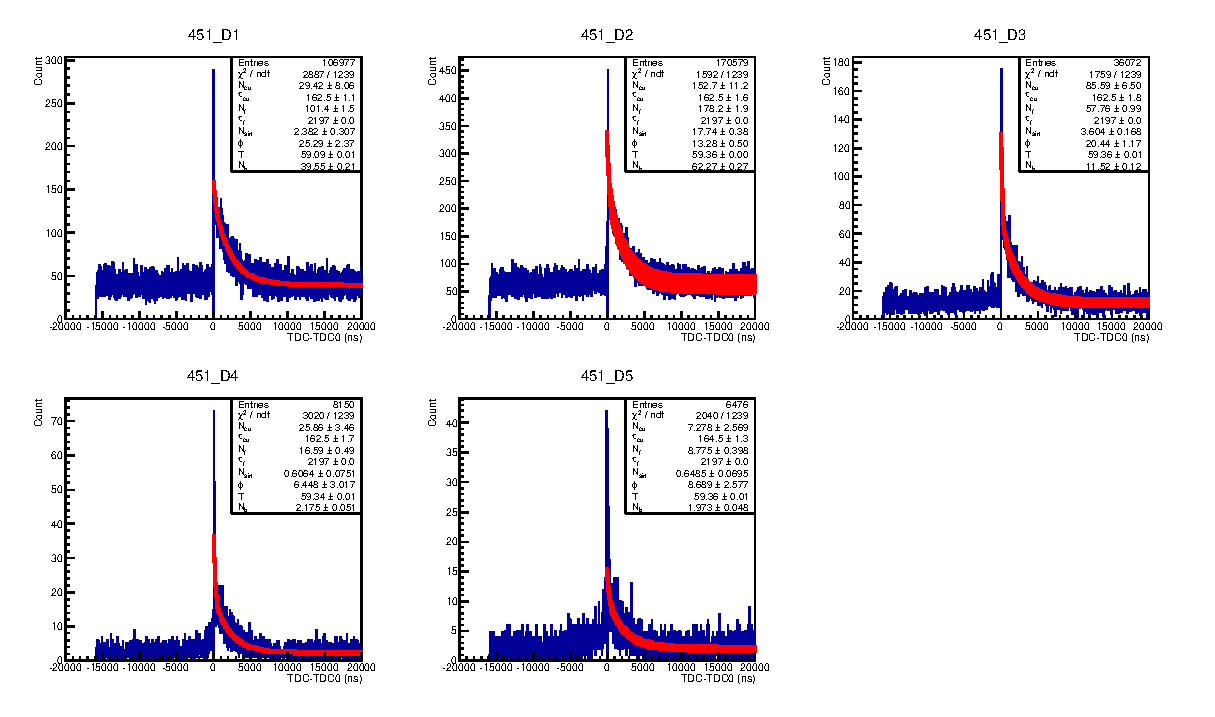
\includegraphics[scale=1]{images/momentum_spectrum/451.eps}
    \caption{Per channel fitting of data for run 451, for this run a 0.5~mm aluminium degrader was used.}
    \label{fig:images_momentum_spectrum_451}
\end{sidewaysfigure}
%
\begin{sidewaysfigure}
    \centering
      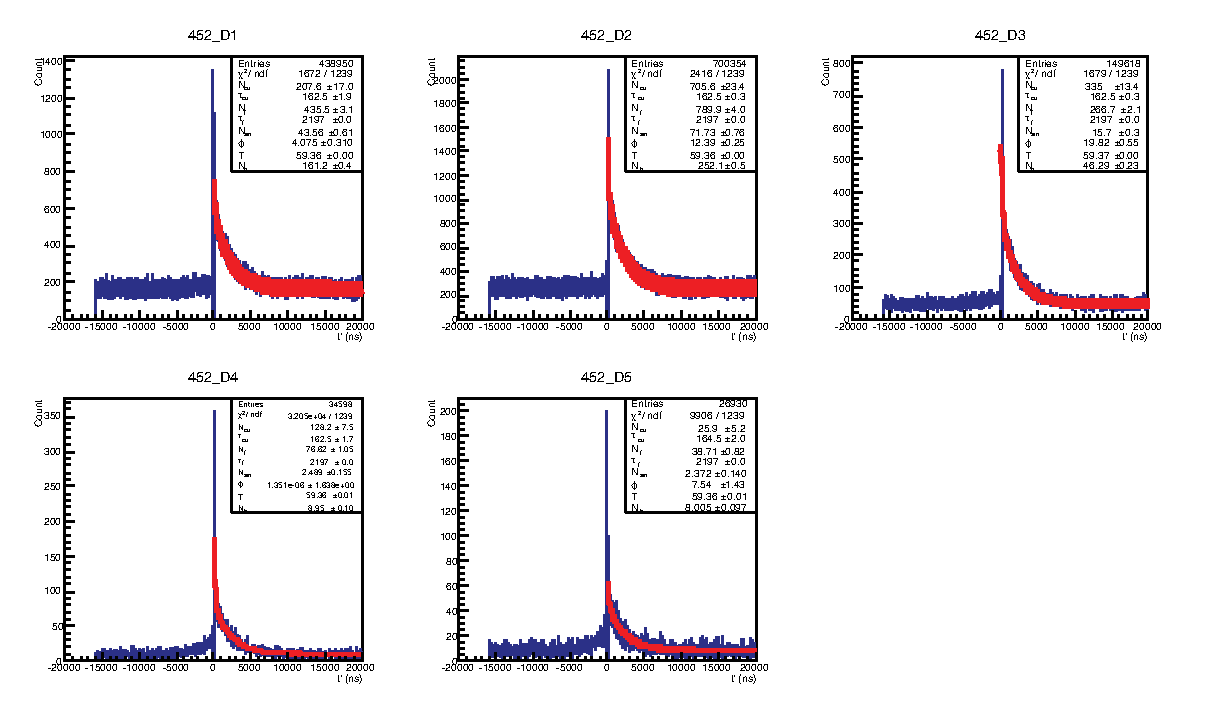
\includegraphics[scale=1]{images/momentum_spectrum/452.eps}
    \caption{Per channel fitting of data for run 452, for this run a 0.5~mm aluminium degrader was used.}
    \label{fig:images_momentum_spectrum_452}
\end{sidewaysfigure}
%
\begin{sidewaysfigure}
    \centering
      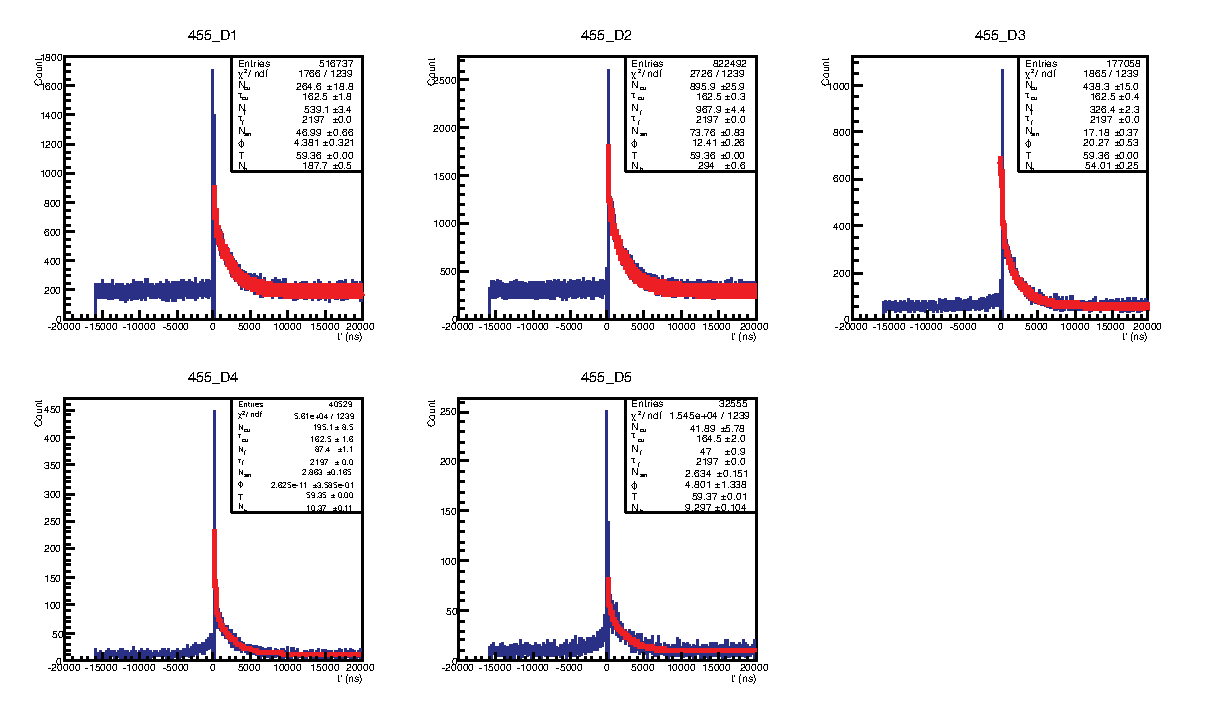
\includegraphics[scale=1]{images/momentum_spectrum/455.eps}
    \caption{Per channel fitting of data for run 455, for this run a 1~mm aluminium degrader was used.}
    \label{fig:images_momentum_spectrum_455}
\end{sidewaysfigure}
%
\begin{sidewaysfigure}
    \centering
      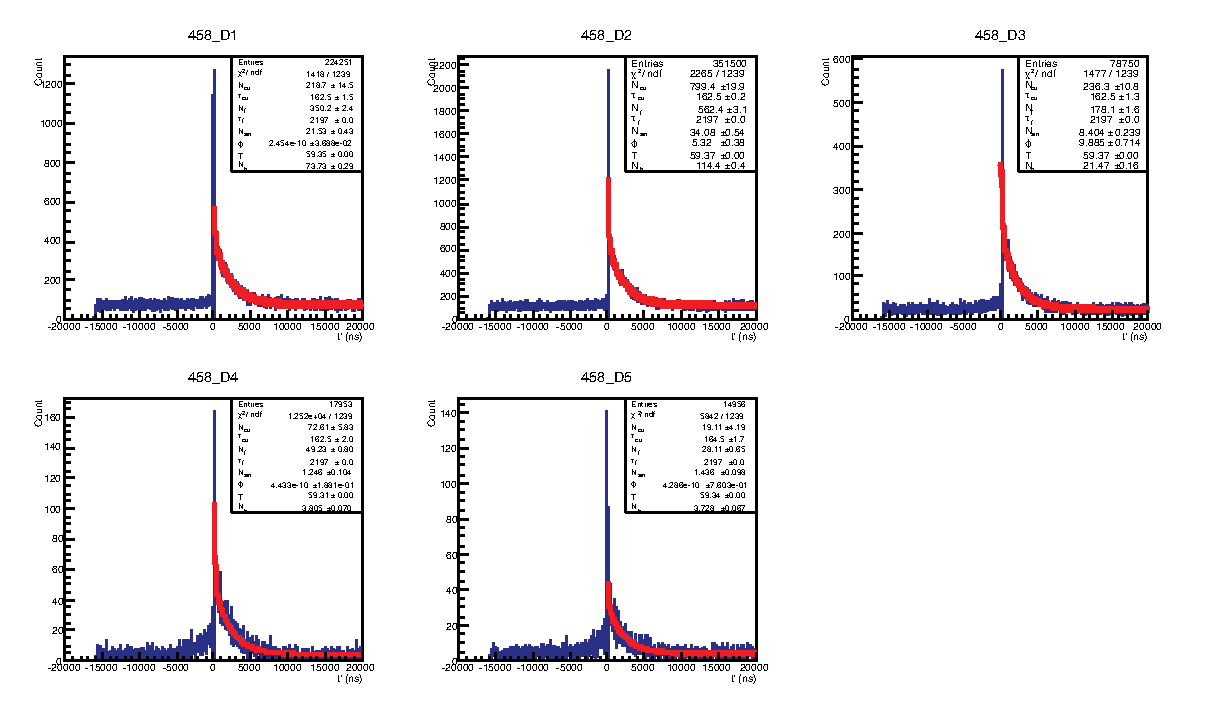
\includegraphics[scale=1]{images/momentum_spectrum/458.eps}
    \caption{Per channel fitting of data for run 458, for this run a 5~mm aluminium degrader was used.}
    \label{fig:images_momentum_spectrum_458}
\end{sidewaysfigure}
%
\begin{sidewaysfigure}
    \centering
      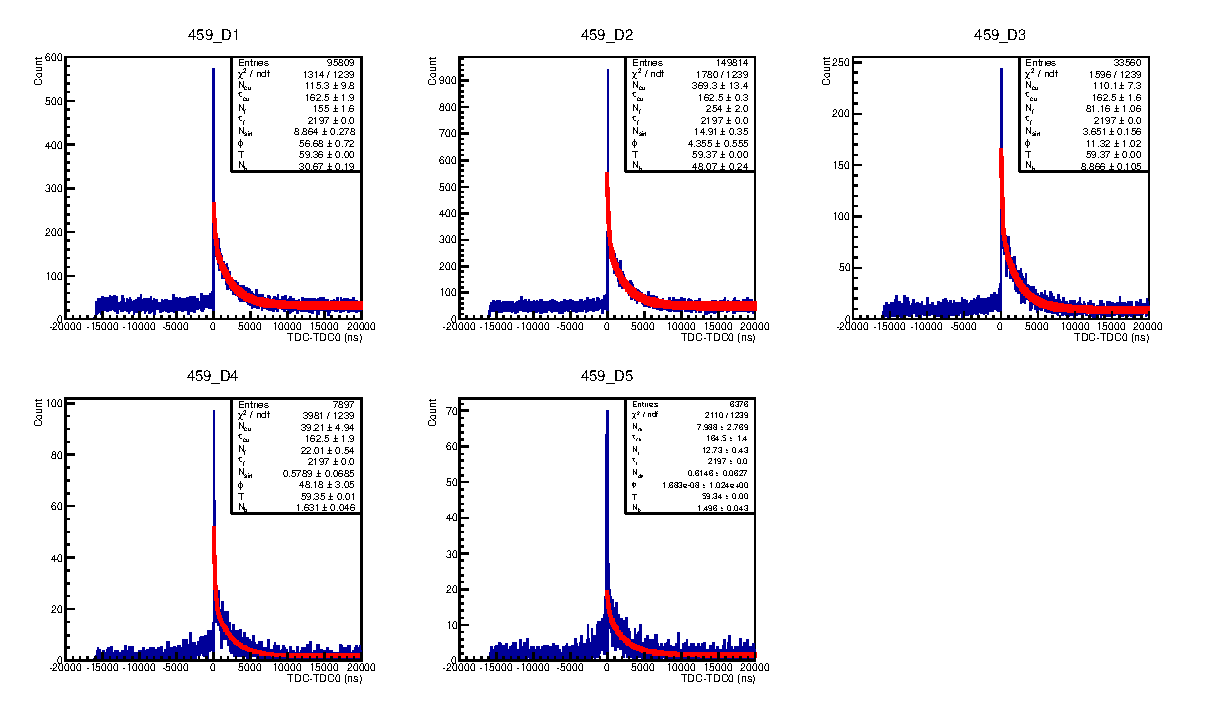
\includegraphics[scale=1]{images/momentum_spectrum/459.eps}
    \caption{Per channel fitting of data for run 459, for this run a 5~mm aluminium degrader was used.}
    \label{fig:images_momentum_spectrum_459}
\end{sidewaysfigure}


\clearpage

Once calculated via integration the number of muons can be summed for all the channels in a run. The summed value can then be normalised between runs to the proton beam current using:
\begin{align}
  R &= \frac{N_{\mu}}{I_p T L} \label{equ:rate}
\end{align}
Where \( R \) is the normalised rate of muon decays (in nA\(^{-1}\)), \(N_{\mu}\) is the number of muon decays (either free or from muonic copper), \( I_p \) is the proton current in nA, \( T \) is the duration of the run in seconds and \(L\) is the live time (as given in table~\ref{tab:dead_time}). The rates and number of muon decays, summed over all channels, are given in table~\ref{tab:rates_res}. The results back up the earlier measurements made on the beam flux (section~\ref{cha:charged_particle_flux}) as the larger values of \(N_f\), \( N_c \) and \(N_b\) are seen in channels D1, D2 and D3, i.e.\ the beam position is in the upper portion of the detector.

\begin{table}
  \begin{center}
  \begin{tabular}{c | c | c | c | r@{\(\pm\)}l | r@{\(\pm\)}l | r@{\(\pm\)}l | r@{\(\pm\)}l  }
    \multirow{2}{*}{Run}  &  \(I_{p}\)  &  \(T\)  &  \multirow{2}{*}{\(L\)}  
         &  \multicolumn{4}{c|}{Copper Decays}   
                                          & \multicolumn{4}{c}{Free Decays}\\
                          &  (nA)       &   (s)   &
         &  \multicolumn{2}{c|}{Count}
                         &  \multicolumn{2}{c|}{ Rate (nA\(^{-1}\))}
                                          &  \multicolumn{2}{c|}{Count}
                                                            &  \multicolumn{2}{c}{Rate (nA\(^{-1}\))} \\
    \hline
    448  &  0.01534  &  9221  &  0.6157  &  19895 & 400  &  228.5 & 4.6   &  528076 & 1283  &  6065 & 15  \\
    451  &  0.01546  &  1001  &  0.7169  &   1999 & 114  &  180.2 & 10.3  &   45269 & 355   &  4080 & 33  \\
    452  &  0.01313  &  4944  &  0.7412  &   9319 & 240  &  193.6 & 5.0   &  200246 & 732   &  4161 & 15  \\
    455  &  0.01332  &  6307  &  0.7613  &  11937 & 265  &  186.6 & 4.1   &  246059 & 803   &  3847 & 13  \\
    458  &  0.01363  &  5144  &  0.8347  &   9365 & 202  &  160.1 & 3.5   &  146384 & 570   &  2502 & 10  \\
    459  &  0.01238  &  2452  &  0.8495  &   4440 & 136  &  172.1 & 5.3   &   65781 & 378   &  2550 & 15  \\
  \end{tabular}
  \end{center}
  \caption{Decay counts and rates, summed over all downstream scintillators.}
  \label{tab:rates_res}
\end{table}

Figures~\ref{fig:images_momentum_spectrum_run_muon_rate_in_f}~and~\ref{fig:images_momentum_spectrum_run_muon_rate_in_cu} show the rates of decays from free muons and muonic copper respectively. These plots are the `pure' rates based solely on the measured values. Between the pairs of runs (e.g.\ runs 451/452 and 458/459) there is reasonable agreement and the general shape suggests that (unsurprisingly) as larger degraders are used there are fewer decays of stopped muons. 

\begin{figure}[hptb]
  \centering
    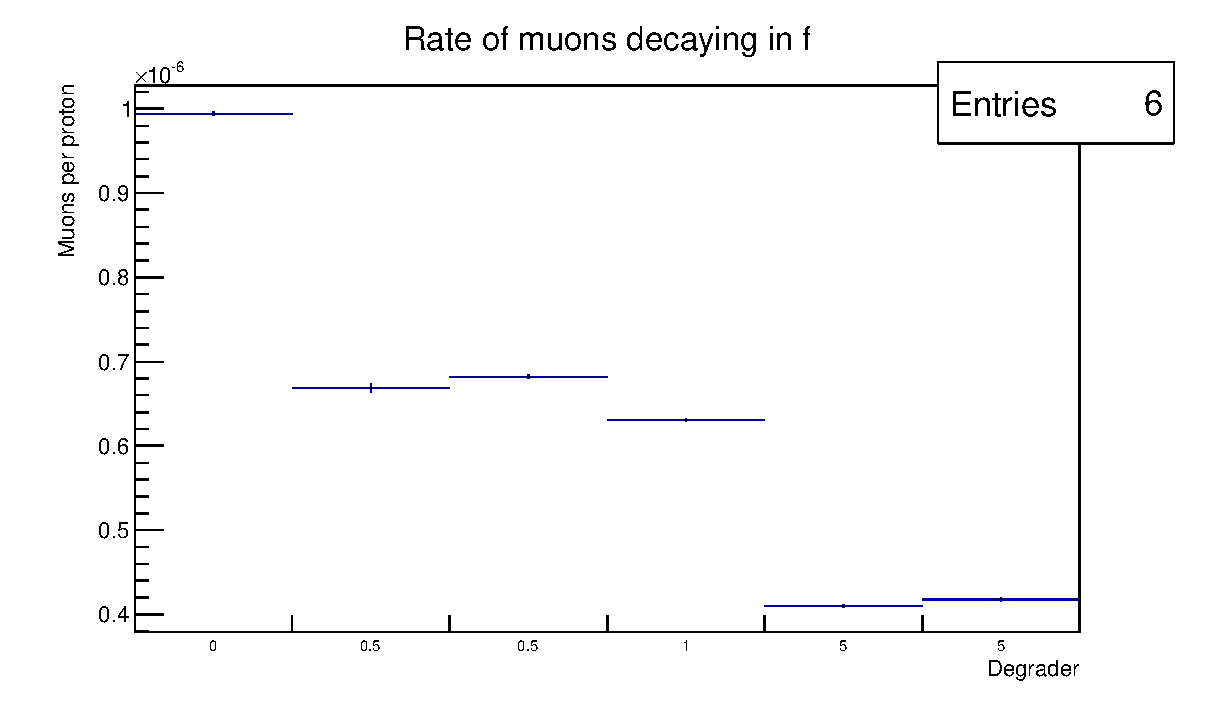
\includegraphics[width=.9\textwidth]{images/momentum_spectrum/run_muon_rate_in_f.eps}
  \caption{Integrated number of free muon decays summed over all channels.}
  \label{fig:images_momentum_spectrum_run_muon_rate_in_f}
\end{figure}

\begin{figure}[hptb]
  \centering
    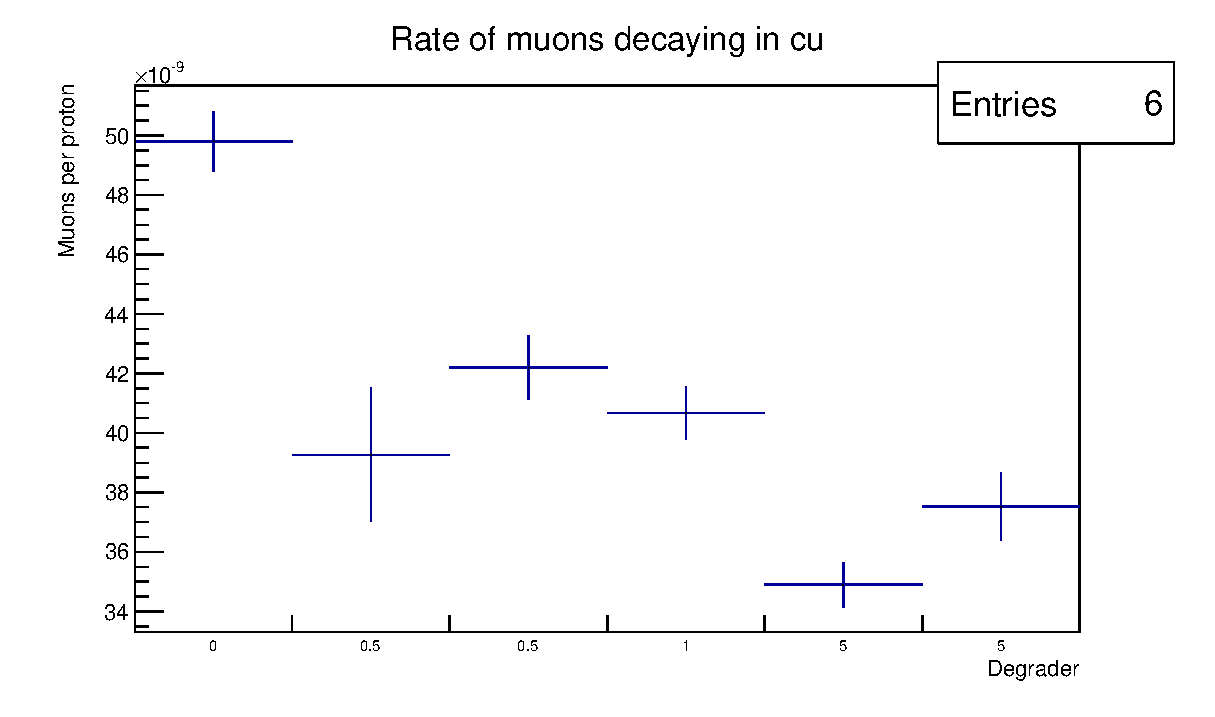
\includegraphics[width=.9\textwidth]{images/momentum_spectrum/run_muon_rate_in_cu.eps}
  \caption{Integrated number of muon decays in copper summed over all channels.}
  \label{fig:images_momentum_spectrum_run_muon_rate_in_cu}
\end{figure}

% As can be seen further refinements can be made to enable more accurate comparison to simulation: inclusion of the acceptance and the detector efficiency as well as conversion of the degrader thickness to the simulated average momentums.

As can be seen in the fit histograms, the \(\chi^2\) values for the fitting of channels D4 and D5 are generally poor and because of this they were removed from the final, summed, rate calculation. The main cause of the poor \(\chi^2\) value is likely the low statistics compounded by the fact that, as the counters share a common trigger those scintillators that are further away from the beam spot will record a greater fraction of noise. Also even for the channels with better \(\chi^2\) values, equation~\eqref{equ:fit} is not a full description of the data. This effect can be seen more clearly when the values for \( \tau_c \) and \( \tau_f \) are also fitted (rather than fixed, as in the analysis). The fitted values for \(\tau_c\) and \(\tau_f\)  are shown in figures~\ref{fig:images_plot_generating_scripts_per_ch_free_lifetime}~and~\ref{fig:images_plot_generating_scripts_per_ch_copper_lifetime} respectively. Both of these plots show that the fitted values differ from the canonical values whilst simultaneously providing a worse \(\chi^2\) than is seen with the constrained values. The poor performance of the fitting when the lifetime values are not fixed is likely a combination of the noisy data and the difficulty of fitting the large number of parameters over a wide range of values (from 1 to 20,000~ns).

\begin{figure}[hptb]
  \centering
    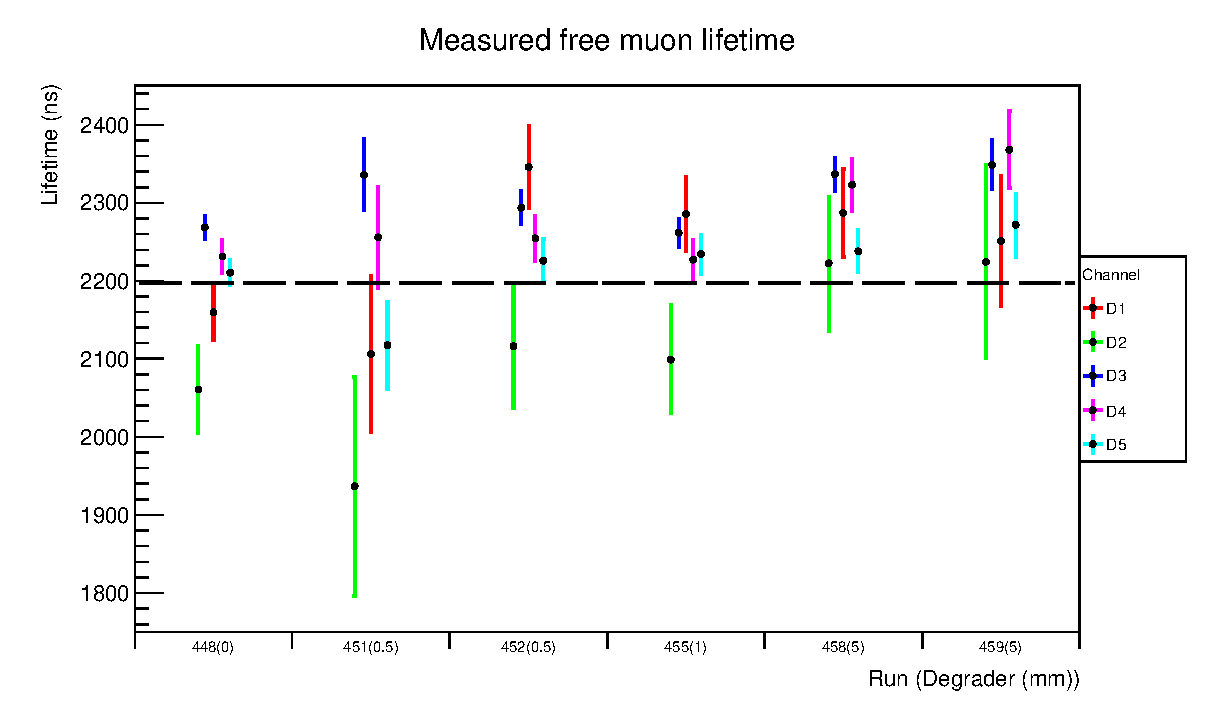
\includegraphics[width=.9\textwidth]{images/plot_generating_scripts/per_ch_free_lifetime.eps}
  \caption{Comparison of fitted value of free muon lifetime for the different channels in each run. The dashed line is the canonical value, \((2.1969811\pm0.0000022)\)~\(\mu\)s~\cite{pdg}.}
  \label{fig:images_plot_generating_scripts_per_ch_free_lifetime}
\end{figure}

\begin{figure}[hptb]
  \centering
    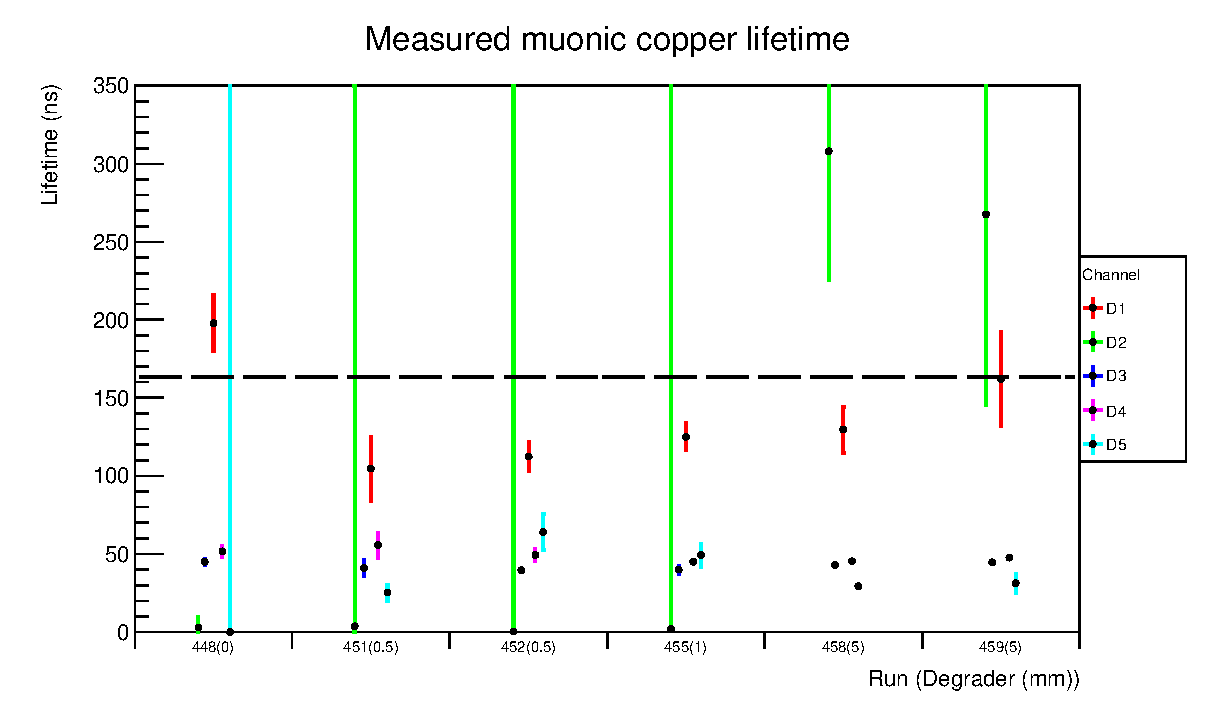
\includegraphics[width=.9\textwidth]{images/plot_generating_scripts/per_ch_copper_lifetime.eps}
  \caption{Comparison of fitted value of muonic copper lifetime for the different channels in each run. The dashed line is the canonical value, \((163.5\pm1)\)~ns~\cite{suzuki_mu_capture_rates}.}
  \label{fig:images_plot_generating_scripts_per_ch_copper_lifetime}
\end{figure}

% \begin{table}
%   \lineup
%   \begin{center}
%   \begin{tabular}{c | c | r@{\(\,\pm\,\)}l | r@{\(\,\pm\,\)}l | r@{\(\,\pm\,\)}l | r@{\(\,\pm\,\)}l | r | l }
%    \multirow{2}{*}{Run} 
%      & \multirow{2}{*}{Channel}
%           &  \multicolumn{2}{c|}{Copper}
%                          &  \multicolumn{2}{c|}{Free}  
%                                           & \multicolumn{2}{c|}{Rate (copper)}
%                                                                  &\multicolumn{2}{c|}{Rate (free)}
%                                                                      &\multicolumn{1}{c|}{\multirow{2}{*}{\(\chi^2\)}}
%                                                                                      & \multicolumn{1}{c}{\multirow{2}{*}{NDF}}  \\ 
%      &    & \multicolumn{2}{c|}{decays}
%                          &  \multicolumn{2}{c|}{decays}  
%                                            & \multicolumn{2}{c|}{(nA\(^{-1}\))}
%                                                                 & \multicolumn{2}{c|}{(nA\(^{-1}\))}
%                                                                                      &         &      \\
%    \hline
%    \multirow{5}{*}{448}
%      & D1 &   4098 & 232  &  184833 & 758  &    47.1\0& 2.7   &  2122.7  &  8.8   &    2772 & 1239  \\
%      & D2 &  11377 & 286  &  259990 & 928  &   130.7\0& 3.3   &  2986\.\0& 11     &    5815 & 1239  \\
%      & D3 &   4420 & 153  &   83253 & 458  &    50.8\0& 1.8   &   956.1  &  5.3   &    2116 & 1239  \\
%      & D4 &   1462 &  85  &   23189 & 228  &    16.79 & 0.98  &   266.3  &  2.6   &  115129 & 1239  \\
%      & D5 &    188 &  59  &   12223 & 183  &     2.16 & 0.68  &   140.4  &  2.1   &   37059 & 1239  \\
%    \hline
%    \multirow{5}{*}{451}
%      & D1 &    220 &  60  &   13602 & 202  &    19.8\0& 5.4   &  1226\.\0& 18    &   2887 & 1239  \\ 
%      & D2 &   1140 &  84  &   23915 & 261  &   102.8\0& 7.6   &  2155\.\0& 24    &   1592 & 1239  \\ 
%      & D3 &    639 &  49  &    7751 & 132  &    57.6\0& 4.4   &   699\.\0& 12    &   1759 & 1239  \\ 
%      & D4 &    193 &  26  &    2227 &  66  &    17.4\0& 2.3   &   200.7  &  6.0  &   3020 & 1239  \\ 
%      & D5 &     55 &  19  &    1178 &  53  &     5.0\0& 1.8   &   106.1  &  4.8  &   2040 & 1239  \\ 
%    \hline
%    \multirow{5}{*}{452}
%      & D1 &   1550 & 128  &   58446 & 413  &    32.2\0& 2.7   &  1214.5  &  8.6  &   1672 & 1239  \\
%      & D2 &   5268 & 175  &  106013 & 538  &   109.5\0& 3.7   &  2203\.\0& 11    &   2416 & 1239  \\
%      & D3 &   2501 & 100  &   35787 & 277  &    52.0\0& 2.1   &   743.6  &  5.8  &   1680 & 1239  \\
%      & D4 &    957 &  57  &   10282 & 141  &    19.9\0& 1.2   &   213.7  &  2.9  &  32046 & 1239  \\
%      & D5 &    196 &  39  &    5195 & 110  &     4.08 & 0.81  &   108.0  &  2.3  &   9906 & 1239  \\
%    \hline
%    \multirow{5}{*}{455}
%      & D1 &   1976 & 142  &   72348 & 453  &    30.9\0& 2.2   &   1131.0 &  7.1  &   1766 & 1239  \\
%      & D2 &   6689 & 194  &  129903 & 589  &   104.6\0& 3.0   &   2030.8 &  9.3  &   2726 & 1239  \\
%      & D3 &   3273 & 112  &   43808 & 304  &    51.1\0& 1.8   &    684.9 &  4.8  &   1865 & 1239  \\
%      & D4 &   1457 &  65  &   11730 & 151  &    22.8\0& 1.0   &    183.4 &  2.4  &  56096 & 1239  \\
%      & D5 &    318 &  44  &    6308 & 121  &     4.97 & 0.69  &     98.6 &  1.9  &  15454 & 1239  \\
%    \hline
%    \multirow{5}{*}{458}
%      & D1 &   1633 & 109  &   46999 & 328  &    27.9\0& 1.9   &    803.4 &  5.7  &   1418 & 1239  \\
%      & D2 &   5968 & 149  &   75477 & 414  &   102.0\0& 2.6   &   1290.2 &  7.2  &   2265 & 1239  \\
%      & D3 &   1765 &  82  &   23907 & 214  &    30.2\0& 1.4   &    408.7 &  3.7  &   1477 & 1239  \\
%      & D4 &    542 &  44  &    6607 & 107  &     9.27 & 0.75  &    112.9 &  1.8  &  12516 & 1239  \\
%      & D5 &    145 &  32  &    3773 &  87  &     2.48 & 0.54  &     64.5 &  1.5  &   5842 & 1239  \\
%    \hline
%    \multirow{5}{*}{459}
%      & D1 &    861 &  74  &   20803 & 216  &    33.4\0& 2.9   &    806.5 &  8.5  &   1314 & 1239  \\
%      & D2 &   2757 & 100  &   34085 & 275  &   106.9\0& 3.9   &   1321.4 & 10.8  &   1780 & 1239  \\
%      & D3 &    822 &  55  &   10893 & 143  &    31.9\0& 2.1   &    422.3 &  5.6  &   1596 & 1239  \\
%      & D4 &    293 &  37  &    2954 &  73  &    11.4\0& 1.4   &    114.5 &  2.8  &   3981 & 1239  \\
%      & D5 &     61 &  21  &    1708 &  58  &     2.35 & 0.81  &     66.2 &  2.2  &   2110 & 1239  \\
%   \end{tabular}
%   \end{center}
%   \caption{Summary of the results of integrating equation~\eqref{equ:fit} and using the values from table~\ref{tab:fit_res}. The rates are the initial values calculated using equation~\eqref{equ:rate}.}
%   \label{tab:rates_res}
% \end{table}

% \begin{figure}[hptb]
%   \centering
%     \includegraphics[width=.9\textwidth]{images/plot_generating_scripts/Ratio.eps}
%   \caption{Ratio of copper to free decays. The X-axis shows the degrader thickness whilst the colour indicates channel.}
%   \label{fig:images_plot_generating_scripts_Ratio}
% \end{figure}

\clearpage
Once the muon rates (figure~\ref{fig:images_momentum_spectrum_run_muon_rate_in_f}) have been calculated they can be corrected to account for other effects. This is shown in figure~\ref{fig:images_plot_generating_scripts_adjusted_muon_rates} where additional terms have been incorporated to account for the photon acceptance, the MPPC efficiency and the systematic errors due to the fitting procedure. 

The photon acceptance was calculated using the optical simulation and a simple muon gun particle source. The photon acceptance was defined to be the ratio of muons that decay in a detectable manner (`potential decays') to those that produce photons that are detected (`detected decays'):
\begin{align}
  A &= \frac{\text{Detected decays}}{\text{Potential decays}} \label{equ:photon_acceptance}
\end{align}
A detectable muon was considered to be one that traverses the upstream detector and has a corresponding daughter electron traverse the downstream detector. The requirement for detected photons are that the number of photons seen exceed the threshold (eight and ten photons for the up and downstream MPPCs respectively, see section~\ref{sub:data_acquisition}). Putting the values from the simulation into equation~\eqref{equ:photon_acceptance}:
\begin{align}
  A &= \frac{8362}{10500} \\
    % &= 77.7\%
    % error calc: =100*(8362/10500)*sqrt(8362/(8362^2) + 10500/(10500^2))
    &= (79.6\pm1.2)\%
\end{align}

The efficiency of any single detector was taken to be the square of the average efficiency of a MPPC, as measured in section~\ref{sec:detector_efficiency}:
\begin{align}
  \epsilon_{\textsc{mppc}}^2 &= (18.6 \pm 4.1)\% 
\end{align}
% Where \(\epsilon_{\textsc{mppc}}\) is the efficiency of a single MPPC from section~\ref{sec:detector_efficiency}. Whilst the efficiency measured was for a different experimental set up and different MPPCs for the final run it was not possible to make a measurement of the efficiency so this acts as a reasonable approximation.

The systematic errors were largely assumed to be due to the inaccuracies in the method of fitting and integrating the data. Sources of this have already been discussed but to quantify it the key values were varied to show the affects of changing the parameters of the fit itself, rather than the parameters that were fitted (e.g.\ \(\tau_f\)). The key parameters were determined to be the point from which the fit was applied (the `lower bound') and the width of the bins used to fit the data. The bin width was varied to 8 and 32~ns whilst the lower bound could only be increased so was changed to 75~ns (there is no data before 50~ns). Using these values all the data was re-fit and the difference from measured value taken. The results are given in table~\ref{tab:systematic_fits}. The maximal fractional differences from the standard measured using 16~ns bins and a 50~ns lower bound were used as the systematic error. The systematic errors were 55.85\% and 1.14\% for copper and free decay counts respectively. As is clear the systematics on the copper fit is much higher but this is what we would expect. The systematic error on the copper count is included in the corrected rate but not for the free rate as the error on the efficiency is the dominant term then.

\begin{table}
  \begin{center}
  \begin{tabular}{c | c | c | c | c | c | c | c | c}
    \multirow{2}{*}{Run}  &  
          Lower       &  Bin         &  \multicolumn{3}{c|}{Copper}     & \multicolumn{3}{c}{Free}       \\
       &  bound (ns)  &  width (ns)  &  Decays & Difference & Fraction  & Decays & Difference & Fraction \\
    \hline
     448  &  \multirow{6}{*}{8}  &  \multirow{6}{*}{50}
              &  228.66  &    0.17  &  0.0007  &  6064.08  &    0.69  &  0.0001 \\ 
     451  & & &  179.62  &    0.54  &  0.0030  &  4080.08  &    0.27  &  0.0001 \\ 
     452  & & &  193.81  &    0.17  &  0.0009  &  4159.70  &    1.28  &  0.0003 \\ 
     455  & & &  186.84  &    0.22  &  0.0012  &  3845.32  &    1.36  &  0.0004 \\ 
     458  & & &  160.44  &    0.35  &  0.0022  &  2502.20  &    0.11  &  0.0000 \\ 
     459  & & &  172.77  &    0.64  &  0.0037  &  2549.44  &    0.79  &  0.0003 \\ 
    \hline
    448  &  \multirow{6}{*}{32}  &  \multirow{6}{*}{50}
             &  184.25  &   44.24  &  0.1936  &  6097.10  &   32.33  &  0.0053 \\ 
    451  & & &  139.95  &   40.21  &  0.2232  &  4103.83  &   24.03  &  0.0059 \\ 
    452  & & &  148.37  &   45.27  &  0.2338  &  4191.79  &   30.81  &  0.0074 \\ 
    455  & & &  141.78  &   44.84  &  0.2403  &  3874.43  &   27.75  &  0.0072 \\ 
    458  & & &  110.46  &   49.63  &  0.3100  &  2530.72  &   28.42  &  0.0114 \\ 
    459  & & &  126.63  &   45.50  &  0.2643  &  2577.57  &   27.34  &  0.0107 \\
    \hline
    448  &  \multirow{6}{*}{16}  &  \multirow{6}{*}{75}
             &  132.05  &   96.44  &  0.4221  &  6047.05  &   17.72  &  0.0029 \\ 
    451  & & &   93.76  &   86.39  &  0.4796  &  4078.37  &    1.43  &  0.0004 \\ 
    452  & & &  105.99  &   87.66  &  0.4527  &  4157.79  &    3.20  &  0.0008 \\ 
    455  & & &   99.67  &   86.95  &  0.4659  &  3846.58  &    0.10  &  0.0000 \\ 
    458  & & &   70.68  &   89.41  &  0.5585  &  2517.28  &   14.97  &  0.0060 \\ 
    459  & & &   84.21  &   87.92  &  0.5108  &  2561.92  &   11.69  &  0.0046 \\
  \end{tabular}
  \end{center}
  \caption{Results of the systematics fits. The maximal values for copper and free decays were taken as the systematic errors for each value (55.85\% and 1.14\% respectively).}
  \label{tab:systematic_fits}
\end{table}

The corrected muon decay rate for material (or freely), \( R_a \), is then:
\begin{align}
    R_a &= \frac{N_{\mu}}{I_p L T A \epsilon_{\textsc{mppc}}^2 } \label{equ:adj_rate}
\end{align}
where the symbols \(I_p\), \(L\) and \(T\) have the same meaning as in equation~\eqref{equ:rate}. The symbols:  \(\epsilon_{\textsc{mppc}}\) and \( A \) are the average efficiency of an MPPC and the photon acceptance respectively. Table~\ref{tab:adjusted_free_decay_rates} shows the results of this calculation and figure~\ref{fig:images_plot_generating_scripts_adjusted_muon_rates} compares it to simulation. As can be seen there is good agreement between the corrected rate of muon decay and what is expected from simulation.

The same protocol can be applied to the muonic copper decays as well as adding the systematic error to get an corrected rate that is shown in figure~\ref{fig:images_plot_generating_scripts_adjusted_muon_rates_cu} and table~\ref{tab:adjusted_cu_rates}. Unfortunately due to the limitations of the simulation not enough negative muons are produced for accurate comparison and so only the measured values are shown here.

\begin{table}
  \begin{center}
  \begin{tabular}{c | c | c | c | c}
    Momentum  & \multirow{2}{*}{Runs}  &  Corrected Rate           &  \multicolumn{2}{c}{Error (nA\(^{-1}\))} \\
     (MeV/c)  &                        &  (nA\(^{-1}\))  &     (incl.\ eff.)  &  (excl.\ eff.)      \\
    \hline
    \(45 \pm 21\)  &       448  &  40,900  &  9,100  &  610  \\
    \(50 \pm 19\)  &  451, 452  &  27,800  &  6,200  &  430  \\
    \(52 \pm 18\)  &       455  &  26,000  &  5,800  &  400  \\
    \(66 \pm 15\)  &  458, 459  &  17,100  &  3,800  &  260  \\
  \end{tabular}
  \end{center}
  \caption{Corrected rates for freely decaying muons. The error column shows the error without the contribution from the MPPC efficiency and with it, as is clear this is the dominant source. The momentum values are the mean and RMS as determined by simulation.}
  \label{tab:adjusted_free_decay_rates}
\end{table}

\begin{table}
  \begin{center}
  \begin{tabular}{c | c | c | c | c | c}
    Momentum  & \multirow{2}{*}{Runs}  &  Corrected Rate  &  \multicolumn{3}{c}{Error (nA\(^{-1}\))}   \\
     (MeV/c)  &                        &  (nA\(^{-1}\))  &  Total  &  (excl.\ sys.)  &  (excl.\ eff.) \\
    \hline
    \(45 \pm 21\)  &       448  &  1,540  &  610  &  340  &  38  \\
    \(50 \pm 19\)  &  451, 452  &  1,260  &  510  &  280  &  43  \\
    \(52 \pm 18\)  &       455  &  1,260  &  500  &  280  &  34  \\
    \(66 \pm 15\)  &  458, 459  &  1,120  &  450  &  250  &  27  \\
  \end{tabular}
  \end{center}
  \caption{Corrected rates of muonic copper decay. Errors are split into three: total error (including systematics and MPPC efficiency); error excluding systematics but including MPPC efficiency; and error excluding both systematic and efficiency contributions (i.e.\ statistical). The momentum values are the mean and RMS as determined by simulation.}
  \label{tab:adjusted_cu_rates}
\end{table}

\begin{figure}[hptb] 
  \centering
    \includegraphics[width=0.8\textwidth]{images/plot_generating_scripts/adjusted_muon_rates.eps}
  \caption{Corrected free muon decay rate and simulated free muon decay rate. The red lines are the simulated results, the blue lines the measured results including the MPPC efficiency error and the black lines are the measured values without the MPPC efficiency error.}
  \label{fig:images_plot_generating_scripts_adjusted_muon_rates}
\end{figure}

\begin{figure}[hptb]
  \centering
    \includegraphics[width=0.8\textwidth]{images/plot_generating_scripts/adjusted_muon_rates_cu.eps}
  \caption{Corrected decay rate of muonic copper. The simulated rates are not shown as the statistics for muonic copper decays were too low to extract reasonable values from. The blue line indicates the error due to systematic error, the red line is the MPPC efficiency error and the black line the statistical error.}
  \label{fig:images_plot_generating_scripts_adjusted_muon_rates_cu}
\end{figure}

\subsection{Analysis} % (fold)
\label{sub:mom_analysis}
As can be seen from figure~\ref{fig:images_plot_generating_scripts_adjusted_muon_rates} there is a good agreement between simulation and experiment. The largest source of errors for this measurement was the lack of accurate information on the detector efficiency and in further measurements this should be corrected. Despite the large errors the data shows a clear reduction in the number of stopped muons as the degrader thickness increases and that this reduction is stable between the repeat measurements. 

Throughout the entire experiment there was a gradual decline in the total trigger rate (even between matched configurations) as is seen in figure~\ref{fig:gain_stability}. The cause of the reduction in trigger rate is unclear, its effect on the results is corrected for through the dead time calculation. 

A point of interest in the data is the difference between the first and subsequent runs. In the first run the simulation predicts a lower rate whilst in all other runs the simulation predicts a higher rate. This suggests that there may be some other effect that needs to be accounted for in either the simulation or the analysis. Another area that needs more accurate modelling is the inclusion of beam effects in order to better understand the sinusoidal noise seen in all data and account for it.

Based on the simulation the stopped muons account for a small portion of the beam, no more than 8~\% of the total muon flux. Using the simulation the fraction of the beam which is stopped for each degrader can be estimated. Using these ratios we can calculate the total muon flux for the RCNP's maximum 1~\(\mu\)A beam:
\begin{align}\label{equ:total_rate}
  T &= 1,000\times\frac{R}{C}
\end{align}
Where \(T\) is the total muon flux per second, \(R\) is the measured muon rate per~nA and \(C\) is the fraction of the beam that was simulated to stop in that configuration. The factor of 1,000 converts from nA to \(\mu\)A and hence to s\(^{-1}\) for a 1~\(\mu\)A proton beam. The calculated values for the total muon flux are shown in table~\ref{tab:total_muon_rates} along with the per~Watt efficiency, using the RCNP's 400~W beam at 1~\(\mu\)A.

\begin{table}
  \lineup
  \begin{center}
  \begin{tabular}{c | r@{\(\pm\)}l | r@{\(\pm\)}l | r@{\(\pm\)}l | r@{\(\pm\)}l}
    Momentum  &  \multicolumn{2}{c|}{Component}
                                  &  \multicolumn{2}{c|}{Rate}
                                                    &  \multicolumn{2}{c|}{Total flux}
                                                                     &  \multicolumn{2}{c}{Efficiency} \\
    (MeV/c)   &  \multicolumn{2}{c|}{(\%)}
                                  &  \multicolumn{2}{c|}{(\(\times10^3\) nA\(^{-1}\))}
                                                    &  \multicolumn{2}{c|}{(\(\times10^8\) s\(^{-1}\))}
                                                                     &  \multicolumn{2}{c}{(\(\times10^5\)~muons~W\(^{-1}\))} \\
    \hline
    448       &  \.8.158 & 0.096  & \042.5 & 13     & \05.21 & 1.62  &   \0\0\013.0 & 4.1  \\
    451       &  \.7.356 & 0.091  & \028.8 & \09.0  & \03.91 & 1.22  &  \0\0\0\09.8 & 3.1  \\
    452       &  \.7.356 & 0.091  & \029.4 & \09.2  & \04.00 & 1.25  &   \0\0\010.0 & 3.1  \\
    455       &  \.6.742 & 0.087  & \027.3 & \08.5  & \04.04 & 1.26  &   \0\0\010.1 & 3.2  \\
    458       &  \.4.665 & 0.071  & \018.0 & \05.6  & \03.86 & 1.20  &  \0\0\0\09.7 & 3.0  \\
    459       &  \.4.665 & 0.071  & \018.4 & \05.7  & \03.94 & 1.23  &  \0\0\0\09.9 & 3.1  \\
  \end{tabular}
  \end{center}
  \caption{Calculated muon production efficiencies and total fluxes at 1~\(\mu\)A. `Component' is the simulated fraction of the total beam that stops in each set up. `Rate' is the sum of the corrected rates for free and copper decays. The total flux was calculated using equation~\eqref{equ:total_rate}. The average total flux is \( (4.16\pm0.92) \times10^8\)~muons~s\(^{-1}\) where the error is the same fractional error as is on the MPPC efficiency, \(\Delta\epsilon_{\textsc{mppc}}^2\sim 22\)~\%. The efficiency is the total flux divided by the full beam power (400~W). The average efficiency of MuSIC is calculated to be \((10.55\pm2.3)\times10^5\)~muons~W\(^{-1}\) which has the same, \(\epsilon_{\textsc{mppc}}^2\) dominated, error as the total flux.}
  \label{tab:total_muon_rates}
\end{table}

Two things are clear from table~\ref{tab:total_muon_rates}: at full power MuSIC should be capable of producing the design goal of \(>10^8\)~muons~s\(^{-1}\) and it should be one of the most intense muon beams in the world. The average intensity, \((4.16\pm0.92)\times10^8\)~muons~s\(^{-1}\), is comparable PSI's most intense muon beam (\(4.8\times10^8\)~muons~s\(^{-1}\)~\cite{mue4_psi}) but achieved with a proton beam significantly less powerful. This last point is best highlighted by comparing the number of muons produced per~Watt of proton beam: PSI produces 292~muons~W\(^{-1}\) whilst MuSIC is predicted to produce \((10.55\pm2.3)\times10^5\)~muons~W\(^{-1}\).

% As has been noted the lack of information on the detector's efficiency was a severe hinderance in the calculation of the muon rate. Further improvements are needed, not only to reduce errors and better understand the detector but to allow testing of the simulation. Work at COMET suggests that there are differences in the particle rates between various simulations (e.g.\ MARS and G4BL), understanding of this will be vital in those measurements.

% subsection mom_analysis (end)


% \chapter{Conclusion} % (fold)
% \label{cha:conclusion}
% %  \(6\times10^8\)~muons/nA)
% Over the course of two years three different measurements of the MuSIC beam-line have been made; each building on the knowledge gathered in the previous. The total charged particle flux was measured and compared to simulation; the muon lifetime was determined and used to confirm their presence; and the number of muon decays under different configurations has been used to determine the momentum flux (as well as the muon flux).
% 
% The three measurements have gone a long way to testing the simulation of MuSIC and to confirming that it is a reasonable approximation to the reality. Further measurements will hopefully refine our knowledge of the beam and maybe begin testing the different models used in the simulation. Work on simulating COMET has already shown that there are differences in the predicted rates of different particles, determining how which simulation is correct will make further work easier and more accurate.
% 
% MuSIC has been shown to perform as expected, producing more muons per proton than any other beam. Even incomplete it's already being used to make new measurements (precisions measurements of decays from muon activated molybdenum) and it is hoped that further funding will help complete this powerful tool. 
% 
% Currently the largest problems with the measurements at MuSIC are in the errors on the measurements but as these are refined more detailed simulations will also be needed. There are two key improvements that can be made to the simulation: larger G4BL run and better digitisation. A larger G4BL run will increase the number of copper stopped muons that will allow detailed investigation of the rates of negative muons stopping in copper, it is also necessary to start making comparisons between different hadron production codes and may provide useful data for refining these at low energy. The second improvement, digitisation, will allow analysis of simulation that's more directly comparable to what's measured. This will be key in understanding backgrounds and having clear understanding of the fine properties of the beam. 
% 

% Over the last three years the simulation of MuSIC has been refined and tuned using data gathered over several periods of beam time. The simulation was written in G4Beamline to cover the bulk portions and Geant4 to test the detectors used. They were also used to compare to the data gathered during the beam-times.
% 
% The three measurements were made over five periods of beam time. Each beam time lasted between 24 and 72 hours. The first measurements were of the charged particle flux, then the muon lifetime was measured and finally the muon momentum distribution was measured. Each measurement was made using simple plastic scintillator detectors with Data Acquisition (DAQ) performed using off the shelf crate systems (NIM, CAMAC and VME). 
% 
% The measurement of the charged particle flux confirmed the beam location to the top and the left of the beam pipe. It also set a benchmark for the particle flux which confirmed the bounds of the maximum muon flux. The measurement determined that the peak particle flux was 90,800\(\pm\)7,000~particles~nA\(^{-1}\) of proton~beam positioned 5~cm above the beam centre (at a distance of 6~cm). The second measurement of the particle flux determined that the beam spot 85~cm from the end of the beam pipe was 25~cm above and 17~cm to the left of the beam centre, with a flux of 10,800\(\pm\)2,100~particles~nA\(^{-1}\). 



% chapter executive_summary (end)

% chapter conclusion (end)
    \part{Clock and Control interface for the Large Pixel Detector} % (fold)
\label{prt:lpd_ccc_interface}

\chapter{Introduction} % (fold)
\label{cha:lpd_ccc_introduction}

\section{Conventions} % (fold)
\label{sec:conventions}
Throughout this document there are several typographical conventions that are observed (see table~\ref{tab:typography}).
% CAPS           = states          e.g. IDLE, 
% bold(CAPS)     = generic         e.g. BUNCH_LENGTH 
% textttt{CAPS}  = commands        e.g. SET_TRIGGER_FLAG
% textttt{lower} = ports/signals   e.g. start_i
% 
% 
% veto from ccc->veto to asic 7 clk
% start from ccc->start to asic 6 clk
% above due to requirements to sync to 4.5 MHz
\begin{table}[htbp]
  \begin{center}
  \begin{tabular}{c|c}
    Type or prefix                  & Meaning                             \\
    \hline                                                   
    \texttt{lower mono-spaced font} & Port or signal names.               \\
    lower normal font               & Port or signal names (tables only). \\
    CAPS                            & Names of generics.                  \\
    \textbf{BOLD CAPS}              & Named states of a state-machine.    \\
    \texttt{MONO-SPACED CAPS}       & Command words.                      \\
    CAPS                            & Command words (tables only).        \\
    0xYYYY                          & Hexadecimal number (YYYY in base 16)\\
    0bYYYY                          & Binary number (YYYY in base 2)      \\
  \end{tabular}
  \end{center}
  \caption{Description of typographic conventions.}
  \label{tab:typography}
\end{table}
% section conventions (end)
%%%%%%%%%%%%%%%%%%%%%%%%%%%%%%%%%%%%%%%%%%%%%%%%%%%


\section{The European X-ray Free-Electron Laser: an overview} % (fold)
\label{sec:xfel_an_overview}
This is a discussion of the work carried out designing and implementing the firmware for the Clock and Control Card (CCC) interface of the Large-Pixel Detector (LPD) for use at the European X-ray Free-Electron Laser (EuXFEL). There will be a brief discussion of EuXFEL, its aims, the detectors and control systems then a more in-depth look at the design, implementation and testing of the interface.

EuXFEL is a 3.4~km Free-Electron Laser (FEL) being constructed below Hamburg, Germany. The project is scheduled to begin operation in 2016 with commissioning beginning in 2015. EuXFEL is built upon expertise and concepts prototyped at the Free-electron Laser in Hamburg (FLASH) which is operated by DESY although EuXFEL will be operated as an independent research facility. The aim of EuXFEL is to produce a coherent X-ray beam with peak brilliance of 10\(^{33}\)~photons/s/mm\(^2\)/mrad\(^2\)/0.1\%~BW; a pulse duration of \( \sim \)100~fs and a wavelength down to \( \sim \)0.1~nm.


\subsection{Synchrotrons and FELs} % (fold)
\label{sub:synchrotrons_and_fels}
X-rays are produced from electrons via synchrotron radiation. When an electron is accelerated through a magnetic field, that causes it to curve and lose energy, this energy is lost as X-rays photons. Synchrotron sources use Linear Accelerators (Linacs) to accelerate electrons before injecting them into a storage ring where they are passed through bending magnets to produce X-rays. The original synchrotron sources used the natural curvature of their storage ring to produce X-rays where more modern designs use special sets of magnets (called `undulators') that very rapidly change the electron's course to produce X-rays. By changing the configuration of the undulators, the X-ray properties can also be adjusted. 

At a FEL very long undulators are used. The long undulators are the key difference that separates FELs from synchrotrons: FEL undulators are tuned so that the electrons undergo `micro-bunching'. Micro-bunching is a process in which the electron bunch interacts with the X-rays it has emitted. As the electrons travel those that lag will receive a boost from the X-rays emitted behind them. Meanwhile, those electrons that lead tend to loose energy via emitted X-rays. As the faster electrons lose energy and the slower electrons gain it the bunch breaks into many smaller bunches. These micro bunches are in phase and produce coherent X-rays. The process of micro-bunching produces X-ray light which, like a laser's, is coherent but it also arrives in very short pulses (\(\mathcal{O}\)(fs)). Whilst lasers are produced through light-amplified stimulated-emission, micro-bunching produces X-rays through Self-Amplified Stimulated-Emission (SASE)\footnote{Technically `FEL' is a misnomer, it should be FES as it is not a laser.}.

 % The properties of these X-rays are the similar to light produced by a Laser, it is coherent but arrive in very short pulses (\(\mathcal{O}\)(fs)). instead of light-amplified they are said to be produced through Self-Amplified, Stimulated-Emission (SASE)\footnote{Technically `FEL' is a misnomer, it should be FES as it is not a laser.}

% The use of undulators is key to producing a FEL, rather than at a synchrotron where they are used just to produce X-rays at a FEL, by adjusting the undulators' properties, the electrons can be forced to interact with the X-rays they emit, through this interaction a single bunch can be forced into many smaller bunches as the slower electrons absorb the X-rays of the faster electrons through a process called `micro-bunching'. Ultimately through micro-bunching the electrons in the beam end up in phase with one-another and rather than LASEing start to self-amplify, stimulated-emission (SASE)\footnote{Technically `FEL' is a misnomer, it should be FES.} this produces a similar effect to a laser in that the resultant light is coherent and with the added bonus of forming very short pulses.
% subsection synchrotrons_and_fels (end)
%%%%%%%%%%%%%%%%%%%%%%%%%%%%%%%%%%%%%%%%%%%%%%%%%%%
\subsection{X-ray production at EuXFEL} % (fold)
\label{sub:x_ray_production_at_euxfel}
At EuXFEL electrons are accelerated to 17.5~GeV using a superconducting linac and the X-rays are produced in one of three SASE undulators which can be combined with conventional undulators to produce photon energies from 25~keV to 0.26~keV which correspond to wavelengths of between 0.05~nm and 4.7~nm. The proposed layout can be seen in figure~\ref{fig:XFEL_layout}. EuXFEL is expected to supply 27,000 pulses of X-ray light (`bunches') per second, with each pulse having a duration of \( \sim \)100~fs. The bunches are split over 10 `trains' per second, each containing up to 2,700 bunches each and lasting \( 600~\mu\)s. The predicted cumulation of all this is a peak brilliance of 10\(^{33}\)~photons/s/mm\(^2\)/mrad\(^2\)/0.1\%BW. For comparison, the energy and peak brilliance of several existing sources (FEL and synchrotron) is given in figure~\ref{fig:xfel-brightness}. As can be seen FELs (FLASH, LCLS) have a much higher peak brilliance although, generally, with a reduced range in energy.
\begin{figure}[htbp]
  \centering
    \includegraphics[width=.9\textwidth]{images/Other/XFEL_layout.png}
    % \includegraphics[width=.9\textwidth]{4_appendix_XFEL/images/Other/XFEL_layout.png}
  \caption{Schematic of the beam-lines for EuXFEL, black denotes electrons whilst red corresponds to X-rays.}
  \label{fig:XFEL_layout}
\end{figure}

\begin{figure}[htbp]
  \centering
    \includegraphics[width=.9\textwidth]{images/Other/XFEL-comparitive_energy-brightness.png}
  \caption{Plot of peak X-ray brilliance against energy for a range of current sources as well as the predicted values for EuXFEL (here labelled `XFEL'). The blue dots show measured peak brilliance for several energies at the existing FLASH facility, `FLASH (seeded)' is a proposed extension using a micro-bunch `seeded' electron beam.}
  \label{fig:xfel-brightness}
\end{figure}

% subsection x_ray_production_at_euxfel (end)
%%%%%%%%%%%%%%%%%%%%%%%%%%%%%%%%%%%%%%%%%%%%%%%%%%%
\subsection{Scientific Motivation} % (fold)
\label{sub:scientific_motivation}
There are two primary problems with more traditional synchrotrons: incoherent light and pulse length. As the light is produced in a long bunch of electrons it has no overall phase. This means that only samples that are crystalline (or can be crystallised, i.e.\ grown into a repeating pattern) can be imaged. Many structures form only poor crystals or can't form them at all. The X-ray pulse length that synchrotrons produce, whilst under normal operating conditions, are generally of order 10--100~ps~\cite{xfel_detector_requirements}. Obviously this places a lower limit on the speed of things that you can `film', again limiting the range of experiments that can be carried out. FELs solve both of these problems by producing coherent light that can have a very short pulse length, additionally because of the SASE process the peak brilliance of a FEL is vastly increased (see figure~\ref{fig:xfel-brightness}).

The primary aim of EuXFEL is to study conditions previously unseen in a laboratory setting. This aim is achieved through three core properties of EuXFEL: `coherence, ultra-high brilliance and time structure'~\cite{xfel_tdr} the combination of these gives access to three broad areas of study: the tiny, the fast and the extreme. Because of the limitations of incoherent light, pulse length and brilliance none of these regimes are easily studied at synchrotrons.

The imaging of the tiny relies on the wavelength of the light used being comparable to the scale of the structure to be imaged. At EuXFEL as well as having X-ray wavelengths sufficient to image molecules, due to the coherent nature of the light non-repeating structures can also be imaged unlike at traditional synchrotrons. Whilst the brilliance of the beam will destroy most samples very quickly, tests at FLASH show that enough time remains to produce a detailed image of the sample, even if it has not been crystallised. This means that larger structures can be imaged at an atomic scale (e.g.\ entire viruses) or structures that won't crystallise or only form very small, low quality crystals (e.g.\ protein membranes).

EuXFEL's time-structure, provides the potential of the second regime, speed. As each individual flash lasts less than \( \sim \)100~fs and each train comprising of 2,700 flashes it's possible to `film' processes as they occur. This will make it possible for researchers to understand what happens during a phase transition or when a material reverses its magnetisation by watching it happen in high detail and without suffering the motion-blur of slower systems.

The final regime, the extreme, is driven by EuXFEL's brilliance. Able to recreate intense temperatures and pressures EuXFEL can ue this to create environments not normally seen on Earth. For example: the propagation of shockwaves through a plasma or to image the stresses on a component under extreme magnetic fields.
% subsection scientific_motivation (end)
% section xfel_an_overview (end)
%%%%%%%%%%%%%%%%%%%%%%%%%%%%%%%%%%%%%%%%%%%%%%%  
\section{Detectors at EuXFEL} % (fold)
\label{sub:detectors_at_euxfel}
In order to achieve EuXFEL's scientific program a broad range of detectors are required. For almost all planned experiments there is a need to image the beam's interaction with the target, the standard solution to this is a 2D pixel detector. This type of detector consists of an array of light sensitive pixels that give both position and intensity information about the incident light, with minor reconstruction an image of the target can then be formed. The basic requirements for the 2D pixel detectors at EuXFEL are~\cite{xfel_tdr}:
\begin{description}
    \item[Swiftness] EuXFEL produces 27,000 X-ray pulses per second, the detector needs to be able to record a large number of these.
    \item[Dynamic range] In any one flash the number of photons received by any portion of the detector can vary massively (between 1 and \(10^5\) photons~\cite{lpd_manual}) this information needs to be preserved with a good signal to noise ratio by the detector.
    \item[Radiation resistance] When fully operational EuXFEL is intended to be used nearly continuously, so obviously any detector used has to be able to survive the harsh environment at the end of the beam-line.
\end{description}

There are currently three 2D pixel detectors being built for use at XFEL: Adaptive Gain Integrating Pixel Detector (AGIPD)~\cite{agipd_spec}, DEPFET Sensor with Signal Compression (DSSC)~\cite{dssc_spec} and Large Pixel Detector (LPD)~\cite{lpd_spec}. All three satisfy the above requirements through a variety of technologies.

The main differences between the three detectors are in their approach to the dynamic range: LPD and AGIPD both have three separate gain levels giving them the required range, whilst DSSC uses the non-linearity of its DEPFET to achieve a similar outcome. There are a few other significant differences: DSSC has hexagonal pixels (AGIPD and LPD have square); AGIPD uses dynamic switching to select the appropriate gain for each pixel before storing it in a single pipeline and LPD has an entire pipeline for each gain level (this means that when a narrower gain is required it can be set and all three pipelines used for storage). 

\subsection{The Large Pixel Detector (LPD)} % (fold)
\label{sub:the_large_pixel_detector_lpd}
LPD is a 2D, 1~Mega-pixel detector designed and build by a collaboration of the Rutherford Appleton Laboratory and Glasgow University in the UK. The detector is designed to be modular with a full 1~Megapixel being made up of 16 `supermodules', each supermodule contains a single Front End Module (FEM) that controls and reads out the 128 Application Specific Integrated Circuits (ASICs) each of which has 512 individual pixels i.e.\ each supermodule is 65,536 pixels divided between 128 ASICs and 1 FEM. It is the FEM that then communicates with the rest of EuXFEL via the Clock and Control Card (CCC) and the Train Builder (TB).
    
There are two lines specified for controlling the ASIC during operation: the system clock (\texttt{clk}) and the control (\texttt{cmd}). The FEM's CCC-interface is responsible for receiving the generic signals from the CCC and converting them to those expected by the ASIC. There are a large number of commands that the ASIC expects in order to function (a full list is given in appendix~\ref{app:asic_command_words}). These commands fall into a few general groups: starts, (no-)vetos\footnote{The ASIC actually uses a `trigger' rather than a `veto', but for consistency with the EuXFEL documentation we will use `no-veto' and `veto' to refer to \texttt{TRIGGER\_FLAG\_SET} and \texttt{NOP} respectively}, stops, resets, and testing. In each of these sets of commands there are generally two or tree individual command words that affect a specific component of the ASIC (e.g.\ reset the write pointer, start the trigger pointer). 
    
Each FEM uses a Xilinx~Virtex-5 Field Programmable Gate Array (FPGA) and two Xilinx~Spartan-3's for control and fan-out, the Virtex-5 has two softcore PowerPC440 processors that manage the resources on the FEM (e.g.\ configuring control registers). As well as the CCC-interface, firmware manages read-out of the ASIC; the ASICs' configuration and communication with the TB. The two Spartan-3 FPGAs are used primarily to co-ordinate fan-out of the signals to the ASICs.
% subsection the_large_pixel_detector_lpd (end)
% section detectors_at_euxfel (end)
\section{DAQ and control systems} % (fold)
\label{sec:daq_and_control_systems}
In a project the scale of EuXFEL there are a large number of different subsystems that need to communicate flawlessly in order to operate. Not only does a single common clock need to be distributed between all systems but it needs to compensate for the time to transmit a signal between the different components and how this latency may change depending on local conditions (e.g.\ the temperature). To maintain synchronicity there are several layers of timing and control system used at EuXFEL. The top-most layer is the master clock from which all other timing signals are derived. The master clock signal is distributed,  along with global information about the machine's status (e.g.\ the next bunch-train's ID), to the Timing Receiver (TR) cards. The 2D detectors use an additional layer (the CCC) to simplify their interface to the TR cards. The CCC removes information that is not needed by the 2D detectors and provides additional information that is received directly from other sub-systems (e.g.\ vetos). In addition to the CCC the 2D detectors share a second common interface, the Train Builder (TB) that provides a common method of storing and ordering data from each train.

The CCC has four primary functions in EuXFEL: 
\begin{enumerate}
  \item Distribution of the clocks required to maintain synchronicity with the rest of the machine.
  \item Control of the attached FEMS.
  \item Providing of veto information for each bunch.
  \item Collection of status information from the FEMs.
\end{enumerate}
In addition to these requirements the CCC can also operate in standalone mode (detached from a TR board) in order to facilitate testing and for use at other locations (e.g.\ LCLS). 

The CCC communicates with FEMs via RJ45 (see figure~\ref{fig:CCC_RJ45_diagram}), the four paired wires carry signals: clock, fast-command, veto and status. The clock signal is a \(\sim\)99~MHz derived from the TR and synchronised to the, \(\sim\)4.5~MHz, bunch clock, the fast command line carries information about each train whilst the veto line carries information on whether a bunch should be kept, the status line returns the received clock to indicate good connections.
\subsection{Clock and Control Card (CCC)} % (fold)
\label{sub:clock_and_control_card}
\begin{figure}[htbp]
  \centering
    \includegraphics[width=.9\textwidth]{images/Other/CCC_RJ45_diagram.png}
    % \includegraphics[width=.9\textwidth]{4_appendix_XFEL/images/Other/CCC_RJ45_diagram.png}
  \caption{The CCC RJ45 wiring diagram. Arrows on the inputs/outputs to FEE indicate signal direction, apart from the status line all are input to the FEE, i.e.\ the status line is the only line expected to send signals from the FEE to the CCC.}
  \label{fig:CCC_RJ45_diagram}
\end{figure}

% subsection clock_and_control_card (end)
\subsubsection{Clock signal} % (fold)
\label{sub:clock_signal}
Rather than a simple monotonic time structure, EuXFEL has two super-imposed patterns: the bunch trains and the bunches. The trains arrive at a rate of 10~Hz with each lasting only 600~\(\mu\)s but containing up to 2,700\( \times\)100~fs bunches, each separated from the next by \(\sim\)220~ns (i.e.\ a rate of \(\sim\)4.5~MHz), figure~\ref{fig:XFEL-time_structure} shows this.
\begin{figure}[htbp]
  \centering
    \includegraphics[width=.9\textwidth]{images/Other/XFEL-time_structure.png}
    % \includegraphics[width=.9\textwidth]{4_appendix_XFEL/images/Other/XFEL-time_structure.png}
  \caption{The timing structure of electrons at EuXFEL and the resultant X-ray pulses. }
  \label{fig:XFEL-time_structure}
\end{figure}

This timing structure forces the detectors to use the time between bunches for data read-out while during the bunch train they are limited to just storing data. This means that each detector is limited by the length of its on-ASIC pipeline with regards to how much data it can store (for LPD this is either 512 frames if using all three gain levels or 1536 if only using one). This structure also means there are two cycles that the detectors need to be synchronised to: the bunch clock (\(\sim\)4.5~MHz) and secondly the bunch-train clock (\(\sim\)10~Hz). Finally, in addition to these two machine-wide clocks there is the common CCC `fast clock' that is used for transmitting commands from the CCC which has a frequency of \(\sim\)99~MHz and is the clock that the ASIC works to.

Note: there is some vagueness as to the exact clock speeds used as, at time of writing a definitive value has yet to be decided on, the bunch clock is expected to remain between 4 and 5~MHz with the fast clock expected to be a simple divisor of this that results in a rate of roughly 100~MHz. 
% subsection clock_signal (end)
\subsubsection{Fast control} % (fold)
\label{sub:control_signal}
The fast control is used to convey information about each train. This information comes in four parts: when the next train will start, when it will stop, what its ID is and what bunch pattern should be used (see section~\ref{sub:veto_signal}, below). There is also a reset command to indicate that the ASIC and FEM should be reset to a known state. 

The expected use of the control signal is shown in table~\ref{tab:fast_commands}, a \texttt{START} signal arrives with attached train ID and bunch pattern ID, after some number of vetos the \texttt{STOP} signal is received. Rarely, either when there is a fault or if, for example, the detector's been switched off, the \texttt{RESET} signal will restore the FEM and ASIC to a prepared state.
\begin{table}[htbp]
  \begin{center}
  \begin{tabular}{c | c | c | c}
    Command  & Bits   & Payload & Description \\
    \hline   
    \multirow{2}{*}{START}    
             & \multirow{2}{*}{0b1100}
                      & Train ID (32b), bunch pattern  & \multirow{2}{*}{Start of the train} \\
             &        & ID (8b), checksum (8b)         & \\
    STOP     & 0b1010 & none                           & End of the train \\
    RESET    & 0b1001 & none                           & Reset the FEM and ASIC \\
    reserved & 0b1111 & n/a                            & n/a\\
  \end{tabular}
  \end{center}
  \caption{Specification of the fast command signals and their payloads.}
  \label{tab:fast_commands}
\end{table}
% subsubsection control_signal (end)
\subsubsection{Veto signals} % (fold)
\label{sub:veto_signal}
Given the previous discussion of the 2D detectors at EuXFEL (section~\ref{sub:detectors_at_euxfel}) it is obvious that it is unfortunately impossible for them to record all 2,700 bunches of the data, equally with a single linac being divided between five, and later ten, experimental stations not every detector will be receiving all of the bunches for every train anyway. To account for this there are two veto systems that allow the detectors to select which bunches they should record for processing: the `bunch pattern' and the `online veto'. Either of these two sources may veto a bunch so it is only recorded if \emph{neither} vetos it. 

The bunch pattern veto is derived from the global configuration of the machine: if, for example, the first half of the electron beam is being sent to another experimental station the detector will receive a pattern that tells it to veto that portion of the train. The patterns act as masks: for each bunch in a train the pattern states whether it should be vetoed or not. The bunch patterns are decided ahead of time, and a selection of patterns\footnote{Predicted to be fewer than 10.} are loaded when the FEM is configured, the bunch pattern to be used for each train is included in that train's header information as part of the start signal sent via the command line.

The online vetos are mainly situational, if the beam doesn't produce any X-rays or there is a fault then there is rarely any point taking data, in which case those bunches should be vetoed. These online vetos can have any source and the signals are supplied to a dedicated veto unit that is external to the CCC. The CCC will in turn pass on the veto or no-veto signal to the FEM of the detector, either with an attached bunch ID or with a fixed latency from the bunch in question depending on the specifications of the detector. Online vetos are what is received via the veto line and they have a format given in table~\ref{tab:veto_spec}, currently LPD makes no use of the bunch ID. The CCC promises that for every bunch either a VETO or a NOVETO signal will be sent, if neither is received then the interface will assume a NOVETO.
\begin{table}[htbp]
  \begin{center}
  \begin{tabular}{c|c|c|c}
    Command & Bits   & Payload                        & Notes\\
    \hline
    VETO    & 0b110  & \multirow{2}{*}{Bunch ID (8b)} & Veto this bunch \\
    NOVETO  & 0b101  &                                & Record this bunch \\
    reserved& 0b111  & n/a                            & n/a \\
  \end{tabular}
  \end{center}
  \caption{Veto signal specification.}
  \label{tab:veto_spec}
\end{table}
% subsection the_clock_and_control_card_ccc (end)
%%%%%%%%%%%%%%%%%%%%%%%%%%%%%%%%%%%%%%%%%%%%%%%
% section daq_and_control_systems (end)
\section{Firmware} % (fold)
\label{sec:firmware}
Firmware describes a broad range of technologies that bridge the divide between hardware (the physical chip and wires) and software (a program intended to run on a processor). Whilst firmware can often be used to refer to quiet complex programs run on embedded systems in this document it is used to refer to the specific logic loaded onto a programmable chip to configure its operation.

As discussed, the LPD FEM uses Virtex-5 FPGAs to run its firmware, FPGAs are made up of `slices' of logic that can be configured in order to create powerful systems. The general layout of a slice is a block of configurable logic attached to a Look Up Table (LUT) this combination provides basic logical manipulations followed by a brute force `if A then B' method of implementing the design. It's important to note that most modern FPGAs have additional dedicated slices that allows them to implement more specialised functions, examples include: digital signal processing, the previously discussed softcore processors, dedicated `Block RAM' (BRAM) etc. The specialised slices mean that software can be used to control configuration settings for the firmware natively which then can run without support from an operating system or creating a custom chip whilst also making use of large optimised structures like BRAM for storage.

\subsection{VHDL} % (fold)
\label{sub:vhdl}
There are a variety of languages for writing firmware, the one used for LPD is VHSIC\footnote{Very High Speed Integrated Circuit} Hardware Description Language (VHDL). VHDL works by describing the expected operation of various discrete blocks within the firmware, these descriptions are then translated (synthesised) into bit-code that, in the case of FPGAs will tell the chip how to configure itself.

Whilst a detailed description of the language are beyond the scope of this document there are several attributes of it that are required to understand the following discussions. The key difference is that VHDL is \emph{description} language. This means that the code exists to describe the mapping from inputs to outputs, how this is actually implemented is left to the compiler. The upshot of this system is that depending on the target being compiled for (e.g.\ FPGA, ASIC, etc.) you can get very different implementations of the same code.

% Whilst a detailed description of the language are beyond the scope of this document there are several attributes of it that are required to understand the following discussions. The first major feature of VHDL to be understood is that it is a \emph{description} language as such the specification makes few guarantees about how any particular block of logic will be implemented as the it ultimately only defines what the inputs and the outputs of a block are, consequentially the same code may produce very different results depending on the synthesiser used and the intended target (e.g.\ FPGA, ASIC, etc.).

The slice-based architecture of FPGAs means that many designs are synthesised as `apply logic to signals' then `look up value of signals in table' and finally `output value stored in table'. The result of this system is that most designs are split into two groups of components the `state-machine' and the `memory'. A state-machine is a set of states with attached conditions, the inputs to the state-machine determine which state should be selected and then that state determines what the output should be, the memory stores any persistent information needed by the state-machine either as input, or output. Throughout CCC-interface firmware there are examples of this where a state-machine implements the logic and a BRAM provides large scale storage.

In VHDL, blocks of code (called `entities') are defined by their name, ports and generics; entities represent a cohesive unit of logic, for example a state-machine. Ports represent in or out-bound signals\footnote{VHDL also specifies `inout' as a bi-directional port but they are not used here.} to that entity, these can either be single or grouped into vectors. The generics of an entity describe constant values associated with it; they can be changed on a per-synthesis scale but not by the firmware itself. Generics are mainly used in the design to specify reset values for registers and values that shouldn't be changeable at run time, but may need to change between systems (e.g.\ delays). 

VHDL specifies two broad classes of value that can be used for ports: signals and vectors, a signal is a single bit of information whilst a vector is a collection of bits in some order. VHDL's basic signal type is called `std\_logic' (sl). std\_logic is generally used for transfer of the boolean values (`1' or `0') but it can also take several other values\footnote{`L', `H', `U', `W', `X', `Z' and `-'.} that better describe the ultimately analogue reality of hardware signals e.g.\ the value `L' specifies a weak signal that should probably be low. The vector form of std\_logic is a `std\_logic\_vector' (slv) that is ordered `X (up)to Y' or `Y downto X', if the slv is converted to a numeric type (e.g.\ an integer) then this ordering determines the `endedness'. E.g.\ if an slv (3 downto 0) is 0b1000 then it has an integer value of 8, the same value but with ordered reversed (i.e.\ 3 to 0) has an integer of 1. Throughout this document order is denoted using parenthesis e.g.\ slv~(3:0) is a std\_logic\_vector~(3~downto~0) while slv~(0:3) is (3~to~0).
% subsection vhdl (end)
%%%%%%%%%%%%%%%%%%%%%%%%%%%%%%%%%%%%%%%%%%%%%%%%%%%
% section firmware (end)
%%%%%%%%%%%%%%%%%%%%%%%%%%%%%%%%%%%%%%%%%%%%%%%

    \ifpdf
\DeclareGraphicsExtensions{.pdf, .jpg, .tif}
\else
\DeclareGraphicsExtensions{.eps, .jpg}
\fi

%%%%%%%%%%%%%%%%%%%%%%%%%%%%%%%%%%%%%%%%%%%%%%%%%%%
\chapter{Design} % (fold)
\label{cha:design}
Design is a two stage process: initial design and designing whilst implementing. Very few large scale projects end up looking exactly like the early designs as use cases change and flaws emerge. To this end it's better to design from a few basic principles and use those to guide the implementation rather than a fixed plan which may, as the implementation progresses, turn out to be wrong.

This chapter discusses the uses cases that were considered for the LPD-CCC interface firmware, the more general principles that guided decisions and finally this chapter discusses the overall design as it was implemented.
\section{Requirements} % (fold)
\label{sec:requirements}
The requirements for the LPD-CCC interface can be split into several groups: those requirements made by EuXFEL/CCC, those that were made by the LPD group and those that emerged as a result of the technology. Whilst most of the requirements of one can be equally seen as requirements of the other by splitting the design based on the source certain design decisions became clearer. This section now discusses these requirements before further discussion of the design.

The first and most obvious requirement is that the interface must correctly interpret the commands received via the four lines that make up the CCC interface and respond appropriately. The firmware also had to remain synchronised with the \(\sim\)4.5~MHz bunch clock to ensure the ASIC recorded data at the correct time. To facilitate this the interface had to respond with a fixed latency to all commands it received. 

LPD requires that the interface can talk to the ASIC via the \texttt{clk} and \texttt{cmd} lines and send the correct word in response to the signal received from the CCC. In order to account for the wrapping nature of the LPD pipeline the FEM was required to log the veto decision for each bunch; without this reconstructing, the time-order of the received images would be a tricky task. To facilitate testing of the LPD ahead of EuXFEL's completion it was also decided that the interface would have to be able to run without an attached CCC in a `single shot' style configuration controlled directly via the softcore processors (which became known as `reset-mode', see section~\ref{sec:transmitter}). A final requirement was that the clock sent to the ASIC had to be adjustable as the v~1.0 of the ASIC required a much slower clock during read-out (by a factor of \( \sim \)100, i.e.\  1~MHz).
% section requirements (end)
%%%%%%%%%%%%%%%%%%%%%%%%%%%%%%%%%%%%%%%%%%%%%%%%%%%
\section{Design Principles} % (fold)
\label{sec:design_principles}
% TODO:xfel design_principles Come back and re-read this!
The main design principles were that the design be modular, flexible and simple. These criteria have many advantages and a few disadvantages, they are also strongly entwined with the pursuit of one often resulting in the development of another. By using these principles the result is a design that not only fulfils the current requirements, but is easy to adapt to future requirements, more maintainable and more understandable.

A modular system is one in which the problem is divided in to smaller units. Each unit should solve one, and only one, problem. Each problem should be made as simple as possible. By creating units in this way they can be developed and tested in isolation which reduces the number of inputs and outputs to be understood. Particularly useful units can then be re-used with less testing and development. The main cost of using modules is that the total solution may not be as efficient as one made from a single entity although developing and testing such a solution may be nearly impossible. 

A good example of this modularity was the control registers. Whilst each version was customised for the specific use case, each one was built from the same core design and once that was established further versions were quick and easy to develop and also had a much lower chance of failure.

The flexibility of a design is strongly coupled to how modular it is. Smaller, simpler, entities are generally more re-useable than larger ones. Obviously at some point the small modules have to be combined and there are certain things that can't be achieved without a certain, minimum amount of complexity. To address this as many aspects of the design as possible were made using VHDLs generics. This meant that the same solution could be used in a number of different situations.

For example, given the number of different clock speeds that might be used with the system, the divisor to convert the fast clock into the bunch clock was set using a generic. By using a generic to describe the ratio of one clock to the other as long as the ratio remains within certain bounds the system can be easily re-configured.

The final principle, simplicity, should be key in making the firmware a long-lived piece of work. Rather than an inflexible, monolithic design that has to be thrown away at the slightest change, hopefully the solution should be easy enough to work with that even if large portions need to be updated the individual changes should be small and easy to make with few (ideally no) unforeseen consequences or dependencies. An example of this is that sections of the receiver entity are already being used to test the prototype CCC.
% section design_principles (end)
%%%%%%%%%%%%%%%%%%%%%%%%%%%%%%%%%%%%%%%%%%%%%%%%%%%
\section{The Design} % (fold)
\label{sec:the_design}
As discussed above each entity should have a clear task and as much as possible a simple interface to achieve it. The overall design process was to break the problem down into ever smaller entities until an entity that encompassed the most basic behaviour was encountered e.g.\ the veto receiver entity de-serialises the veto information and checks it for commands. Certain entities couldn't be fully decomposed without introducing non-uniform latencies. This was especially true for implementing the veto logic in the transmitter entity, in such cases the core requirements won out over design principles.

Ultimately the design was split into three sections: receiver, transmitter and the veto filter. The receiver entity is designed to read the signals from the CCC, process them and flag which words it had received. The veto filter combines the bunch pattern, maximum number of writes the ASIC can make and veto signals whilst logging the decisions. Finally the transmitter interprets the flags set by the other two entities and send the correct word to the ASIC.

Each section used a state-machine for the logic. The veto-filter and transmitter also used BRAM and registers for large scale storage and configuration. In each entity, the number of signals in or out, was minimised to avoid confusion. Softcore access to the BRAMs and registers was done via a standardised 32b Remote Direct Memory Access (RDMA) interface. Communication with the other firmware units was implemented using std\_logic flags apart from the transfer of header information via LocalLink to the read-outt entity.
% section the_design (end)
%%%%%%%%%%%%%%%%%%%%%%%%%%%%%%%%%%%%%%%%%%%%%%%%%%%
% chapter design (end)
%%%%%%%%%%%%%%%%%%%%%%%%%%%%%%%%%%%%%%%%%%%%%%%%%%%
\chapter{Implementation} % (fold)
\label{cha:implementation}
As discussed in chapter~\ref{cha:design} the top level design was split into three entities: receiver, veto-filter and transmitter. Each entity has its own section (below) split into an introduction on the aims of the entity; a description of its interface including generics; what registers it uses and any format information; and finally discussion of how the entity was implemented. 

The interface of the entity describes in and out ports as well as any generics that it uses, `LocalLink' and `RDMA' refer to the collection of ports that make up a pre-defined interface (see appendices~\ref{app:local_link_interface} and \ref{app:rdma_interface} respectively). The five attributes (`in', `out', `generic', `LocalLink' and `RDMA') are grouped together under the description `direction' in the following tables.\footnote{Except in the top level description where the generics are in a separate table.}

The registers section of an entity describes any memory locations that can be accessed via the softcore, what is stored in them and what (if any) format that data is expected to be in (e.g.\ some control registers will consist of multiple bits used to flag specific use cases). The implementation sections discuss the design decisions and intended use of each entity as well any possible limitations (e.g.\ some BRAMs can overflow causing undefined behaviour if incorrectly set).

\section{Top level} % (fold)
\label{sec:top_level}
The top level of the CCC interface consists of three core and two ancillary entities. The receiver, the transmitter and the veto filter form the core and a delay unit with associated configuration register form the ancillary entities. A schematic of this can be seen in figure~\ref{fig:ccc_interface_entity}. 

\begin{figure}[htbp]
  \centering
  \includegraphics[width=\textwidth]{images/pdfs/ccc_interface_block.pdf}
  \caption{Top level block diagram. The \texttt{clk} and \texttt{rst} signals are supplied to each block and have been elided from block diagrams unless otherwise noted.}
  \label{fig:ccc_interface_entity}
\end{figure}

\subsection{Interface} % (fold)
\label{sub:top_interface}
The top level interface is given in table~\ref{tab:top_ccc_interface}, the generics for the top level are discussed in section~\ref{sub:top_generics}. As can be seen, the interface is fairly simple: the received clock, an asynchronous reset, then the two in-ports from the CCC (command and veto), two out-ports to the ASIC, four flags for use within the FEM, a set of RDMA interfaces to the softcore and a LocalLink combined with the \texttt{nvetos\_sent} bus to the read-out entity in order to form the packet to send to the TB.
\begin{table}[htbp]
  \begin{center}
    \begin{tabulary}{\textwidth}{l | c | c | L}
      Name                          & Direction & Type & Description \\
      \hline
      clk                           & \multirow{4}{*}{in} 
                                      & sl & Fast clock, generally from CCC.                                 \\
      rst                           & & sl & FEE internal reset signal.                                      \\
      cmd\_from\_ccc                & & sl & Serial CMD line from CCC.                                       \\
      veto\_from\_ccc               & & sl & Serial VETO line form CCC.                                      \\
      \hline
      cmd\_to\_asic                 & \multirow{2}{*}{out}
                                      & sl               & AKA `asic\_in' at ASIC.             \\
      clk\_to\_asic                 & & sl               & AKA `clk\_in' at ASIC.              \\
      \hline
      rsync\_sent\_flag             & \multirow{5}{*}{out}
                                      & sl               & See section~\ref{sub:tx_interface}  \\
      readout\_sent\_flag           & & sl               & \dittostraight                      \\
      downscaler\_start\_sent\_flag & & sl               & \dittostraight                      \\ 
      downscaler\_stop\_sent\_flag  & & sl               & \dittostraight                      \\ 
      nvetos\_sent                  & & slv (8:0)        & \dittostraight                      \\ 
      \hline
      ll                            & \multirow{6}{*}{Interface}
                                      & LocalLink & Access to the veto log.                                         \\
      delay\_reg                    & & RDMA      & Set the internal delays, see section~\ref{sub:top_registers}    \\
      tx\_cmd\_bram                 & & RDMA      & See section~\ref{sub:tx_registers}.                             \\
      tx\_ctrl\_reg                 & & RDMA      & \dittostraight                                                  \\
      pattern\_bram                 & & RDMA      & See section~\ref{sub:veto_registers}.                           \\
      pattern\_id\_reg              & & RDMA      & \dittostraight                                                  \\
    \end{tabulary}
  \end{center}
  \caption{Top level interface for the clock and control interface.}
  \label{tab:top_ccc_interface}
\end{table}
% subsection interface (end)

\subsection{Generics} % (fold)
\label{sub:top_generics}
To provide maximum flexibility (as well as minimum repetition) all generics are available at the top level and are automatically propagated to all entities that use them. There are four generics that are specific to the top level: \textbf{START\_}, \textbf{STOP\_}, \textbf{RESET\_}, and \textbf{VETO\_START\_} (all suffixed with `\textbf{DELAY\_RST}', see table~\ref{tab:all_generics} for a full list of generics). These generics set the \emph{reset} values for the delay registers (see table~\ref{tab:delay_regs}) i.e.\ should the \texttt{rst} signal be asserted then the values that register will have afterwards are specified by these generics. A detailed description of what these registers do is given below in section~\ref{sub:top_registers}.
\begin{table}[htbp]
  \begin{center}
    \begin{tabulary}{\textwidth}{l| c | c | L}
      Name                       & Type       & Entities       & Notes \\
      \hline
      WORD\_LENGTH               & integer    & TL, V, T        & Length of ASIC command words, default:22.    \\
      MAX\_NVETOS                & integer    & TL, V, T        & Maximum of no-vetos to accept, default:512.  \\
      N\_BUNCHES                 & integer    & TL, V, T        & Number of bunches in a train, default:3072.  \\ 
      \hline
      START\_DELAY\_RST          & slv (31:0) & TL              & (default: 0x00000001)                \\
      STOP\_DELAY\_RST           & slv (31:0) & TL              & (default: 0x00000001)                \\
      RESET\_DELAY\_RST          & slv (31:0) & TL              & (default: 0x00000001)                \\
      VETO\_START\_DELAY\_RST    & slv (31:0) & TL              & (default: 0x00000055)                \\
      \hline                                                        
      START\_WORD                & slv (3:0)  &  R              & From CCC, (default: 1100)           \\
      STOP\_WORD                 & slv (3:0)  &  R              & From CCC, (default: 1010)           \\
      RESET\_WORD                & slv (3:0)  &  R              & From CCC, (default: 1001)           \\
      VETO\_WORD                 & slv (2:0)  &  R              & From CCC, (default: 110)            \\
      NO\_VETO\_WORD             & slv (2:0)  &  R              & From CCC, (default: 101)            \\
      BUNCH\_ID\_LENGTH          & integer    &  R              & Bunch ID length (default:12)        \\
      TRAIN\_ID\_LENGTH          & integer    &  R              & Train ID length (default:32)        \\
      CHECKSUM\_LENGTH           & integer    &  R              & Checksum length (default:8)         \\
      BUNCH\_PATTERN\_LENGTH     & integer    &  R              & Bunch pattern ID length (default:8) \\
      \hline                                                    
      PATTERN\_REG\_(0:9)\_RESET & slv (31:0) &  V              & Reset values for the pattern register.\\
      \hline                                                    
      REG\_RESET\_(9:0)          & slv (31:0) &  T              & Register resets (0-9). \\
      SYNC\_RESET\_SIG           & slv (31:0) &  T              & Flag that the \texttt{SYNC\_RESET} command has been sent.   \\
      READOUT\_SIG               & slv (31:0) &  T              & Flag that the \texttt{READOUT} command has been sent.       \\
      DOWNSCALE\_SIG             & slv (31:0) &  T              & Flag to start the down-scaler (either internal or external).\\
      DOWNSCALER\_STOP\_SIG      & slv (31:0) &  T              & Flag to stop the down-scaler.                               \\
      DOWNSCALE\_FACTOR          & integer    &  T              & Factor for the internal down-scaler, default: 100.          \\
    \end{tabulary}
  \end{center}
  \caption{A table of the generics used in the design, their type, name, where they are used (R=receiver, V=veto-filter, T=transmitter, TL=top-level).}
  \label{tab:all_generics}
\end{table}

% subsection top_generics (end)
\subsection{Registers} % (fold)
\label{sub:top_registers}
There is only one register in the top level that is accessible; it is used for control of delays between the receiver and other entities. The 32b register provides delays of up to \( 2^{32} - 1 \)~clocks for the three signals sent to the transmitter entity (i.e.\ \texttt{start}, \texttt{stop} and \texttt{reset}) and the delaying of the \texttt{start} signal to the veto filter, i.e.\ that forms the \texttt{veto\_start}. The appropriate delay for `veto\_start' is given by:
\begin{equation}\label{equ:veto_start_delay}
  \begin{split}
  \text{VETO\_START\_DELAY} =&~\text{START\_NWORDS} \times                   \\
                             &~\text{WORD\_LENGTH} + \text{START\_DELAY} - 2  
  \end{split}
\end{equation}
Where \texttt{START\_NWORDS} is the number of words (as set in the transmitter control register) to be sent to the ASIC in response to the \texttt{START} command (including any \texttt{NOPS} required to delay the actual start), \textbf{WORD\_LENGTH} is the length in bits of each of those words (set via generic) and \texttt{START\_DELAY} is any further delay added between the receiver and the transmitter, the `\(- 2\)' accounts for the internal delay of the veto filter. 
    
There is no delay register to control the veto signals themselves as these are assumed to be wanted with minimum latency.
    
\begin{table}[htbp]
  \begin{center}
    \begin{tabular}{c | c | c }
      Name               & Address & Default    \\
      \hline
      START\_DELAY       & 0x1     & 0x00000001 \\
      STOP\_DELAY        & 0x2     & 0x00000001 \\
      RESET\_DELAY       & 0x3     & 0x00000001 \\
      VETO\_START\_DELAY & 0x4     & 0x00000055 \\
    \end{tabular}
  \end{center}
  \caption{Summary of the top level delay registers. The default can be overridden via the generics (section~\ref{sub:top_generics}).}
  \label{tab:delay_regs}
\end{table}
% subsection registers (end)
\subsection{Implementation} % (fold)
\label{sub:top_implementation}
A schematic of the entities at the top level is shown in figure~\ref{fig:ccc_interface_entity}. There are two broad paths through the system: command and veto. The command path is delayed to allow offsets to be accounted for whilst the veto path is kept as fast as possible. It's also worth noting that the veto filter receives two start signals, one to indicate that the train ID and bunch pattern ID have been received and a second to indicate when the first veto will arrive, both of these signals are derived from the same start signal but the later has to be carefully timed to coincide with the beginning of vetos.

% subsection top_implementation (end)
% section top_level (end)
%%%%%%%%%%%%%%%%%%%%%%%%%%%%%%%%%%%%%%%%%%%%%%%%%%%
\section{Receiver} % (fold)
\label{sec:receiver}
As stated in the introduction there are five signals that are sent by the CCC, these are transmitted via two ports: the \texttt{cmd\_from\_ccc} and the \texttt{veto\_from\_ccc}. The CCC \texttt{clk} carries the derived fast clock (normally 99~MHz) which is synchronised to the slow machine clock (normally 4.5~MHz) which is distributed by the timing receiver. The full list of commands and payloads can be seen in table~\ref{tab:ccc_commands}. As the receiver block is expected to be static during operation (i.e.\ not need any configuration) only generics are used and there are now externally accessible registers.
\begin{table}[htbp]
  \begin{center}
  \begin{tabular}{c | c | c | c}
    Name     & Value  & Payload & Notes \\
    \hline
    START    & 0b1100 & 48b     & Start of the train \\
    STOP     & 0b1010 & n/a     & End of the train \\
    RESET    & 0b1001 & n/a     & Reset the FEM and ASIC \\
    \hline
    VETO     & 0b110  & 8b      & Veto this bunch \\
    NO-VETO  & 0b101  &         & Record this bunch \\
  \end{tabular}
  \end{center}
  \caption{The full set of commands received from the CCC. The payload for the \texttt{START} is the train ID (32b), the bunch pattern ID (8b) and a check-sum (8b). The (\texttt{NO-})\texttt{VETO} payloads are the same, the 8b bunch ID.}
  \label{tab:ccc_commands}
\end{table}

\subsection{Interface} % (fold)
\label{sub:rx_interface}
The top level interface for the receiver entity is shown in table~\ref{tab:rx_interface}. Of the generics, only the word definitions should be changed and only then for words of the same length (e.g.\ `110' changed for `101'). The payload values can be made shorter but not longer.
    
The in ports are essentially the same as the CCC specification with the addition of an internal asynchronous \texttt{rst} line which will clear any buffers and return the state-machines to IDLE.
    
The outputs give a single line for each command as well as buses that hold payload values until overwritten. It's important to note that the command lines go high for only a single clock whilst the payload buffers will retain their value until the next command starts, this means that, for example, the train\_id will remain available until the \texttt{STOP} command begins to be received.
\begin{table}[htbp]
  \begin{center}
    \begin{tabulary}{\textwidth}{l|c|c|L}
      Name          & Direction & Type       & Description \\
      \hline
      START\_WORD            &  &  slv (3:0) & Default serial command: 1100\\
      STOP\_WORD             &  &  slv (3:0) & Default serial command: 1010         \\
      RESET\_WORD            &  &  slv (3:0) & Default serial command: 1001         \\
      VETO\_WORD             &  &  slv (2:0) & Default serial command: 110          \\
      NO\_VETO\_WORD         &  &  slv (2:0) & Default serial command: 101          \\
      BUNCH\_ID\_LENGTH      &  &  integer   & Expected bunch ID length (default:12)\\
      TRAIN\_ID\_LENGTH      &  &  integer   & Expected train ID length (default:32)\\
      CHECKSUM\_LENGTH       &  &  integer   & Expected checksum length (default:8) \\
      BUNCH\_PATTERN\_LENGTH & \multirow{-9}{*}[11.5pt]{Generic} 
                                &  integer   & Expected bunch pattern ID length (default:8) \\
      \hline
      clk          & \multirow{4}{*}{in}  & sl                & CCC clock \\
      rst          &   & sl                & FEE internal reset              \\
      cmd\_i       &   & sl                & Fast command line from CCC      \\
      veto\_i      &   & sl                & Fast veto line from CCC         \\
      \hline
      start\_o     & \multirow{8}{*}{out} & sl                & Start signal to transmitter     \\
      stop\_o      &  & sl                & Stop signal to transmitter      \\
      rst\_o       &  & sl                & Reset signal for transmitter    \\
      veto\_o      &  & sl                & Veto to trigger veto filter     \\
      no\_veto\_o  &  & sl                & No veto to trigger veto filter  \\
      bunch\_p\_o  &  & slv (7:0)  & Bunch pattern ID to veto filter \\
      bunch\_id\_o &  & slv (7:0)  & Bunch ID to veto filter         \\
      train\_o     &  & slv (31:0) & Train ID to veto filter         \\
    \end{tabulary}
  \end{center}
  \caption{Top level interface of the receiver entity.}
  \label{tab:rx_interface}
\end{table}
% subsection interface (end)
\subsection{Implementation} % (fold)
\label{sub:rx_implementation}
The receiver module is split into two state machines, one for each of the two command lines, as seen in figure~\ref{fig:rx_entity}. The entities have similar designs although the command receiver entity is slightly more complex to cope with the non-constant, multi-part payloads. 
\begin{figure}[htbp] 
  \centering
  \includegraphics[scale=1]{images/pdfs/rx_block.pdf}
  \caption{Block diagram of the receiver entity.}
  \label{fig:rx_entity}
\end{figure}
  
The designs uses strobes to signal which type of command has been received and buses to hold the ID information. The ID-buses (train, bunch pattern, checksum and bunch) are cleared at the start of the next command, this means that the data is available until it gets replaced.
  
The two entities use simple state-machines designs (figures~\ref{fig:cmd_rx_flow} and \ref{fig:veto_rx_flow}) that can be summarised as: `IDLE \( \rightarrow \) LOG\_COMMAND \( \rightarrow \) STROBE\_COMMAND \( \rightarrow \) [LOG\_PAYLOAD \( \rightarrow \)] IDLE'. For both command and veto lines the state machine is triggered by the line going high. The stream is de-serialised by passing the serial commands to a shift register. Once a command is matched then the appropriate strobes is set. If the command has an attached payload then that is passed to a shift register until the appropriate number of payload bits have been received when they are written to a bus and the machine returns to `IDLE'.
\begin{figure}[htbp]
  \centering
  \includegraphics[width=0.7\textwidth]{images/pdfs/cmd_rx_flow.pdf}
  \caption{Flow diagram of the command receiver. The serial signals are read and flags set as required. The `START' payload i.e.\  train ID, bunch pattern ID and checksum) are stored and remain available until cmd\_i next goes high i.e.\  the start of the next command).}
  \label{fig:cmd_rx_flow}
\end{figure}
\begin{figure}[htbp]
  \centering
  \includegraphics[width=0.5\textwidth]{images/pdfs/veto_rx_flow.pdf}
  \caption{Flow diagram of the veto receiver entity. This de-serialises and splits the veto signals into the command and its payload, the Bunch id.}
  \label{fig:veto_rx_flow}
\end{figure}

As every command on the \texttt{veto} port has the same format:
\begin{align}
  <\texttt{COMMAND} 3:0><\texttt{BUNCH~ID} 11:0>
\end{align}
the veto receiver (figure~\ref{fig:veto_rx_flow}) only implements two states: CMD and BUNCH\_ID with the command (either VETO or NO-VETO) being flagged once it's received and the Bunch ID being recorded regardless. In the command receiver (figure~\ref{fig:cmd_rx_flow}) there are five states: IDLE, CMD, TRAIN, BUNCH\_PATTERN and CHECKSUM. The TRAIN, BUNCH\_PATTERN and CHECKSUM are used to record the \texttt{START} command's payloads. If the \texttt{STOP} or \texttt{RESET} commands are received, the flow returns to IDLE to await the next command. 
% subsection implementation (end)
% section receiver (end)
%%%%%%%%%%%%%%%%%%%%%%%%%%%%%%%%%%%%%%%%%%%%%%%%%%%
\section{Veto Filter} % (fold)
\label{sec:veto_filter}
As discussed in section~\ref{sub:veto_signal} there are two sources of vetos that needed be combined: the bunch pattern and the online sources. It is assumed that 10 bunch patterns will be sufficient for general operation. The LPD, due to its fixed pipeline size, has a third source of vetos: only 512 bunches can be recorded.\footnote{Unless running with a single gain setting.} A general truth table is given in table~\ref{tab:veto_truth_table}, as can be seen a \texttt{NO-VETO} is only sent if fewer than the maximum \texttt{NO-VETOS}s have been sent and both the pattern and the veto line agree to specify that a \texttt{NO-VETO} should be sent.
    
\begin{table}[htbp]
  \begin{center}
    \begin{tabular}{r|r|r||r}
      Line  & Pattern &   Count   & Outcome \\
      \hline
      veto  &   veto  & \(>\) Max & veto    \\
      nveto &   veto  & \(>\) Max & veto    \\
      veto  &  nveto  & \(>\) Max & veto    \\
      nveto &  nveto  & \(>\) Max & veto    \\
      \hline
      veto  &   veto  & \(<\) Max & veto    \\
      nveto &   veto  & \(<\) Max & veto    \\
      veto  &  nveto  & \(<\) Max & veto    \\
      nveto &  nveto  & \(<\) Max & no-veto \\
            
    \end{tabular}
  \end{center}
  \caption{Truth table for veto decisions. Count is the number of `no-veto's already sent, it is assumed to be 512 but can be any number less than this.}
  \label{tab:veto_truth_table}
\end{table}

\subsection{Interface} % (fold)
\label{sub:veto_interface}
The interface for the veto filter is given in table~\ref{tab:veto_interface}. There are ten generics to be set that specify the reset values for the pattern ID register (see section~\ref{sub:pattern_id_registers}).
    
The in ports are mainly concerned with signals from the receiver module, these are used to determine when vetos should be expected as they need to be synchronised with the bunch clock. There are two start signals that are of concern: the \texttt{veto\_start} and \texttt{start\_i}, the former of these indicates when the first veto should be expected whilst the latter indicates that the \texttt{START} command, the train~ID and the bunch~pattern~ID have been received. The train and bunch~pattern~IDs are required before the first veto is received in order to correctly load the veto pattern as well as create the header for the veto logger. The bunch~ID is received but, currently, nothing is done with it. The \texttt{stop\_i} signal is used as an alternative to the maximum number of bunches to stop the veto filter.
    
The out ports are very simple, one is the final veto decision which is sent to the transmitter whilst the other is a count of the number of \texttt{NO-VETO} commands sent to the ASIC. The number of no-vetos is required for the read-out entity to know how many words to expect once read-out starts.
    
There are 3 data interfaces which are discussed in section~\ref{sub:tx_registers}. Briefly: the two RDMA interfaces allow external access to the pattern BRAM and the pattern ID register whilst the LocalLink interface is used by the read-out entity to access the veto-decision-log which is required for data reconstruction.
    
\begin{table}[htbp]
  \begin{center}
    \begin{tabulary}{\textwidth}{l|c|c|L}
      Name & Direction & Type & Description \\
      \hline 
      WORD\_LENGTH               & & integer                   & Length of ASIC command word (default: 22).           \\
      MAX\_NVETOS                & & integer                   & Number of n\_vetos we can send (default: 512).       \\
      N\_BUNCHES                 & & integer                   & Maximum number of bunches in a train (default: 3072).\\
      % PATTERN\_REG\_(0:9)\_RESET & & slv (31:0) & Reset values for the pattern register (default: see~\ref{sub:veto_registers}). \\
      PATTERN\_REG\_(0:9)\_RESET &  \multirow{-4}{*}[-11.5pt]{generic} 
                                   & slv (31:0) & Reset values for the pattern register (default: see~\ref{sub:veto_registers}). \\
      \hline
      clk                & \multirow{10}{*}[-5.75pt]{in}  
                           & sl                & CCC clock.          \\
      rst                & & sl         & Internal FEE reset.                             \\
      veto\_i            & & sl         &                                                 \\
      nveto\_i           & & sl         &                                                 \\
      start\_i           & & sl         &                                                 \\
      stop\_i            & & sl         &                                                 \\
      veto\_start        & & sl         & Delayed start signal to coincide with vetos.    \\
      bunch\_id          & & slv (11:0) & Not actually used.                              \\
      train\_id          & & slv (31:0) & Added to the local link header.                 \\
      bunch\_pattern\_id & & slv (7:0)  & Used to select the veto pattern.                \\
      \hline   
      veto\_to\_tx       & \multirow{2}{*}[-11.5pt]{out} 
                            & sl                & Combined pattern and veto decision.             \\
      nvetos\_sent       &  & slv (8:0)  & Need to know how much to read from the ASIC.    \\
      \hline
      pattern\_bram\_rdma     & \multirow{3}{*}[-23pt]{interface} 
                                 & RDMA      & Interface to the pattern entity RAM, mask: 0x000003FF \\
      pattern\_id\_reg\_rdma  &  & RDMA      & Interface to the pattern ID/BRAM offset registers, mask: 0x0000000F. \\
      ll                      &  & LocalLink & Interface to the veto log FIFO, uses a 256b data bus. \\
    \end{tabulary}
  \end{center}
  \caption{Interface for the veto filter.}
  \label{tab:veto_interface}
\end{table}
% subsection veto_interface (end)
\subsection{Registers} % (fold)
\label{sub:veto_registers}
In the veto filter there are two memory blocks: the pattern ID registers and pattern BRAM, both accessed via a dedicated RDMA interface and the veto log which is accessed via local link (see appendices~\ref{app:rdma_interface} and~\ref{app:local_link_interface}). 
\subsubsection{Pattern BRAM} % (fold)
\label{sub:pattern_bram}
The pattern BRAM holds the pre-defined veto patterns. These are combined with the fast veto line to decide whether or not to veto a bunch i.e.\  a bunch can be vetoed by either the pattern \emph{or} the veto line). Each pattern consists of a bit for each bunch in a train (it is assumed that there will be \( < \)3,072 bunches in each train). If the corresponding bit is `1' then the bunch will be vetoed, otherwise it is dependent on the veto line.
  
It is assumed that no more than ten patterns will be needed in normal operation so the BRAM is configured to hold 1,024\( \times  \)32b words. This means that for a 3,072 bunch train 96 words need to be defined for each pattern. The pattern is assumed to be spread across monotonically increasing addresses (e.g.\ address 0x0 to 0x60), the veto bits are applied 0 to 31. 
% subsubsection pattern_bram (end)
\subsubsection{Pattern ID registers} % (fold)
\label{sub:pattern_id_registers}
The pattern ID registers map IDs to their appropriate offset within the BRAM. There is no specification for the number of patterns needed during normal operation but 10 registers are assumed to be enough. The value of each register must be of the format:
\begin{align} \label{fmt:pattern_id}
  <\text{PATTERN\_ID } 31:24>\ldots<\text{BRAM offset } 9:0> 
\end{align}
Default values for the register are given in table~\ref{tab:default_pattern_id_reg}, the reset values are set via generics at the top level and the current value can be changed via RDMA. The defaults assume that the patterns are all unique with no overlap, as such each delimitates 96\( \times \)32b wordsi.e.\  3,072 bunches. If there is an intersection between the end of one pattern and the start of another then setting the offset to the beginning of the common section will work as expected.
\begin{table}[htbp]
  \begin{center}
    \begin{tabular}{c|c|c|c}
      Register & Value      & Pattern ID & Offset \\
      \hline
      0x1      & 0x01000000 & 0x1        & 0x000  \\ 
      0x2      & 0x02000060 & 0x2        & 0x060  \\  
      0x3      & 0x030000C0 & 0x3        & 0x0C0  \\ 
      0x4      & 0x04000120 & 0x4        & 0x120  \\ 
      0x5      & 0x05000180 & 0x5        & 0x180  \\ 
      0x6      & 0x060001E0 & 0x6        & 0x1E0  \\ 
      0x7      & 0x07000240 & 0x7        & 0x240  \\ 
      0x8      & 0x080002A0 & 0x8        & 0x2A0  \\ 
      0x9      & 0x09000300 & 0x9        & 0x300  \\ 
      0xA      & 0x0A000360 & 0xA        & 0x360  \\ 
    \end{tabular}
  \end{center}
  \caption{Default reset values for pattern ID registers.}
  \label{tab:default_pattern_id_reg}
\end{table}
% subsubsection pattern_id_registers (end)
\subsubsection{Veto log} % (fold)
\label{sub:veto_locallink}
The veto log is a 13\( \times \)256b FIFO which logs the veto decision for each bunch. This information is formed into a LocalLink frame which uses 256b data words. The 256b header is defined as:
\begin{equation}\label{fmt:ll_header}
  \begin{split}
  <\text{Train ID } 255:224>&<\text{Bunch Pattern ID } 223:216>\ldots              \\
                           \ldots&<\text{Number of no-vetos sent } 191:182> \ldots
  \end{split}
\end{equation}
where `\( \dots \)' represent padding (1s). The rest of the frame consists of the veto log which consists of a bit per bunch indicating either a veto (`1') or a no-veto (`0'). The entities are ordered MSB first, e.g.\ bit 255 of frame 0 indicates the first veto decision whilst bit 0 of frame 12 indicates the last decision. 
% subsubsection veto_locallink (end)
% subsection veto_registers (end)
\subsection{Implementation} % (fold)
\label{sub:veto_implementation}
The veto filter is split into two distinct processes: filtering and logging. Filtering is a requirement of the specification. The logging is required because the ASIC records no identifying information about each bunch and due to the ASIC's write pointer wrapping through memory, images are not guaranteed to be read out in chronological order; a block diagram of this solution is shown in figure~\ref{fig:veto_filter_entity}.
    
\begin{figure}[htbp]
  \centering
  \includegraphics[width=0.7\textwidth]{images/pdfs/veto_filter_block.pdf}
  \caption{Block diagram of the veto filter. Note: \texttt{veto\_start} is the start signal synchronised to the vetos, \texttt{start} is the \texttt{START} signal from the Rx block and used to load the bunch pattern.}
  \label{fig:veto_filter_entity}
\end{figure}
    
The  1,024\( \times \)32b BRAM is used to store the veto patterns to be combined with the veto signal in order to form the veto decisions. To construct the veto decision and control access into the BRAM a state machine implementing figure~\ref{fig:veto_filter_flow} was used. The veto decisions are made at the beginning of each word to reduce latency whilst BRAM and state changes are made at the end. The final entity, the pattern ID register, exists to specify the mapping from bunch pattern ID to BRAM offsets.
    
\begin{figure}[htbp]
  \centering
  \includegraphics[width=0.8\textwidth]{images/pdfs/veto_filter_flow.pdf}
  \caption{Flow diagram of the veto filter.}
  \label{fig:veto_filter_flow}
\end{figure}
    
The logging is performed using a simple state machine to feed in words to a 32b in, 256b out first in, first out BRAM (FIFO), this state machine (figure~\ref{fig:veto_logger_flow}) also constructs the LocalLink frame header (the train ID, the bunch ID then `0' padding). The header requires 8 clocks between \texttt{start\_i} being asserted and \texttt{veto\_start}, to be properly formed. The FIFO is a simple First Word Fall Through (FWFT) entity with the optional \texttt{empty} and \texttt{almost\_empty} signals enabled. The read out of the FIFO is performed via a 256b-word LocalLink interface. Once either \texttt{stop\_i} is asserted or \texttt{N\_BUNCHES} have been counted any remaining bits of the 256b word are filled with `1's and the LocalLink's \texttt{src\_rdy} is asserted. 
    
The LocalLink interface is implemented by wrapping the FIFO's 256b \texttt{data\_out} port in some simple logic to make it conform to the local link standard. This mainly involves using \texttt{empty} to monitor the state of the FIFO, \texttt{almost\_empty} as \texttt{eof} and an internal flag from the logging state-machine for the \texttt{sof}. The \texttt{sop} (start-of-payload) signal is not used to differentiate the header from the payload as the entire frame will ultimately form part of the meta-data in the header of the read-out.
    
\begin{figure}[htbp]
  \centering
  \includegraphics[width=0.8\textwidth]{images/pdfs/veto_logger_flow.pdf}
  \caption{Flow diagram for the veto decision logger.}
  \label{fig:veto_logger_flow}
\end{figure}

% subsection veto_implementation (end)
% section veto_filter (end)
%%%%%%%%%%%%%%%%%%%%%%%%%%%%%%%%%%%%%%%%%%%%%%%%%%%
\section{Transmitter} % (fold)
\label{sec:transmitter}
The transmitter entity's main task is to act as the interpreter for the signals received from the CCC, translating them into command sequences that the ASIC can understand and act upon. As has been discussed above there are four signals that need to be translated for the ASIC: \texttt{START}, \texttt{STOP}, \texttt{RESET} and (\texttt{NO-})\texttt{VETO}. The first three command signals all require an arbitrary number of words be sent to the ASIC whilst the veto signals are responded to by one of two words.
    
The transmitter can run in one of two mode; `dynamic veto mode' and `reset mode'. Dynamic veto mode is intended to be the normal mode of operation for XFEL whilst reset mode is intended for static runs with simple veto patterns (e.g.\ for testing). A comparison of the two can be seen in table~\ref{tab:dynamic_vs_reset_mode}. Reset mode is enabled by strobing bit 0 of the main control register (see section~\ref{sub:ctrl_reg} for details). The transmitter also has an optional minor mode called `down-scaler mode'; this is primarily for v~1.0 of the ASIC that requires a slower clock duringread-outt. When enabled it uses a multiplier (set by generic) to slow the clock, after a set number of cycles normal speed is resumed. 
    
\begin{table}[htbp]
  \begin{center}
    \begin{tabular}{r | X{2.5cm} | X{2.5cm} }
      & \multicolumn{2}{c}{Mode} \\
      & Dynamic-veto & Reset \\
      \hline
      Standalone operation   & \xmark & \cmark \\
      Dynamic veto decisions & \cmark & \xmark \\
      \multirow{4}{*}{Signal response}
      & START  & \multirow{4}{*}{Register flag} \\
      & STOP   & \\
      & RESET  & \\
      & N/VETO & 
    \end{tabular}
  \end{center}
  \caption{Comparison of dynamic veto and reset modes.}
  \label{tab:dynamic_vs_reset_mode}
\end{table}

\subsection{Controlling the ASIC} % (fold)
\label{sec:controlling_the_asic}

The LPD ASIC manual~\cite{lpd_manual} specifies the command sequences required for each stage of operation of the ASIC. For the veto commands a simple selection between \texttt{NOP} (veto) and \texttt{TRIGGER\_FLAG\_SET} (no-veto) is required. The other commands have more complex sequence sets that can change based on operation; a brief summary will be given here and full details can be found in the LPD ASIC manual~\cite{lpd_manual}. 

The standard response to the START command is to set the ASIC in a state ready to write to its memory, this means resetting the write and trigger points and clearing the skip register. Once these commands have been carried out the ASIC will start incrementing the write pointer through the memory locations. After additionally starting the trigger pointer, the ASIC is ready to write the contents of the pixels when a \texttt{TRIGGER\_FLAG\_SET} (i.e.\ NO-VETO) is received. 

The command sequence for the STOP command is more complex and split over two stages: the pre and postread-outt sections. To start read-out the ASIC is set in a stable mode thus:
\begin{enumerate}
  \item The ASIC is put in power saving mode.
  \item Read out of the data begins.
  \item Disable on-chip resets.
  \item Manually reset the gain, pre-amp, write and trigger pointers.
\end{enumerate}
The data read back consists of one 36b word for each no-veto sent, once all of these have been sent the ASIC is returned to ready mode for the next train:
\begin{enumerate}
  \item Power up the ASIC, i.e.\ return bias currents to full.
  \item Re-synchronise the ASIC to the bunch (\( \sim \)4.5~MHz) clock.
  \item Re-enable on chip resets.
  \item Stop read out.
\end{enumerate}
\textbf{Note:} the above constitute a basic over view of the STOP process, there are some important considerations with regards to synchronisation of these commands that are beyond the scope of this and covered in full in the LPD ASIC manual~\cite{lpd_manual}.

The ASIC command words have the format:
\begin{align}\label{fmt:asic_format}
  <\text{SYNC }19><\text{X }18<\text{CMD } 17:10><\text{PADDING\_ZEROS } 9:0>
\end{align}
if a word length greater than 20b is being used (e.g.\ 22b, the current default) then the zero-padding is extended as required. The `SYNC' bit is a `1' and `X', by convention, a `0'; these are automatically prepended by the state machine. The only exception to this is the 20b command \texttt{SYNC\_RESET} (currently set to be 0x5A5A5) which overrides the above format.

% section controlling_the_asic (end)
\subsection{Interface} % (fold)
\label{sub:tx_interface}
The transmitter has three `sets' of generics: the control register reset values, the flag words (ending in \texttt{\_SIG}) and the down-scaler factor. The register resets set the default value to be written to the assorted registers if \texttt{rst} is asserted. The flag words specify certain command words that the transmitter should scan for in order to flag them for use elsewhere. The \texttt{SYNC\_RESET} flag is intended for use with any entities (e.g.\ the slow command line) that have to be synchronised to the ASIC's bunch clock. The \texttt{READOUT} is intended for use by the Read-out entity in order to prepare for read-out. The \texttt{DOWNSCALER\_SIG} is used to begin either the internal (if it's enabled) or an external down-scaler clock. The \texttt{DOWNSCALER\_STOP\_SIG} is only for use by an external source (the internal version counts clocks). The \texttt{DOWNSCALER\_FACTOR} specifies the factor to use for the internal down-scaler e.g.\ a factor of 100 means a scale of 100 fast clock cycles to each slow clock.
    
The in ports to the transmitter are all flags from the receiver; with the standard exception of \texttt{rst} which is the FEM internal signal (cf.\ \texttt{reset} which is the flag from the receiver).
    
The out ports fall into 3 categories: signals to the ASIC (\texttt{ASIC\_in} and \texttt{clk\_in}), flags (marked \texttt{\_sent}) and \texttt{start\_nwords\_o}. The ASIC commands are defined in the specification. The flags have been discussed above with regards to their generic-defined trigger words. The final out port is a wrapper to the value of the \texttt{start\_nwords} register (see section~\ref{sub:tx_registers}) which is used in setting the delay for \texttt{veto\_start}.
    
The two RDMA interfaces are used for access to the command sequence BRAM and the control registers (sections~\ref{sub:tx_bram} respectively).
    
\begin{table}[htbp]
  \begin{center}
    \begin{tabulary}{\textwidth}{l | c | c | L}
      Name & Direction & Type & Description \\
      \hline
      REG\_RESET\_(9:0)     & & slv (31:0) &  Register resets (0-9). \\
      SYNC\_RESET\_SIG      & & slv (31:0) & Flag that the \texttt{SYNC\_RESET} command has been sent.                 \\
      READOUT\_SIG          & & slv (31:0) & Flag that the \texttt{READOUT} command has been sent.               \\
      DOWNSCALE\_SIG        & & slv (31:0) & Flag to start the down-scaler (either internal or external).\\
      DOWNSCALER\_STOP\_SIG & & slv (31:0) & Flag to stop the down-scaler.                               \\
      DOWNSCALE\_FACTOR     & \multirow{-6}{*}[11.5pt]{Generic} % Avoids extra newline at top
      % DOWNSCALE\_FACTOR     & \multirow{-16}{*}[11.5pt]{Generic} % Avoids extra newline at top
                              & integer    & Factor for the internal down-scaler, default: 100.          \\
      \hline
      clk   & \multirow{6}{*}{in} 
               & sl & The CCC clock.          \\
      rst   &  & sl & FEE reset.              \\
      start &  & sl & From the receiver entity.\\
      stop  &  & sl & \dittostraight          \\
      reset &  & sl & \dittostraight          \\
      veto  &  & sl & From the veto filter.   \\
      \hline
      % asic\_in                & \multirow{7}{*}[-28.75pt]{out}
      asic\_in                & \multirow{7}{*}{out}
                                 & sl                & Fast serial commands to the ASIC.  \\
      clk\_in                 &  & sl                & Clock to the ASIC.  \\
      readout\_sent           &  & sl                & Read-out flag (for ASIC receiver entity).  \\
      rsync\_sent             &  & sl                & \texttt{SYNC\_RESET} flag (for slow control entity).  \\
      downscaler\_start\_sent &  & sl                & Downscaler start flag.  \\
      downscaler\_stop\_sent  &  & sl                & Downscaler stop flag.  \\
      start\_nwords\_o        &  & slv (31:0) & Number of words used for `START' to set veto\_start delay.\\
      \hline
      bram\_rdma & \multirow{2}{*}[-17.25pt]{Interface} 
      & RDMA & Interface to the ASIC command word BRAM. Mask: 0x000003FF. \\
      ctrl\_rdma & & RDMA & Interface to the control register. Mask: 0x0000000F. \\
    \end{tabulary}
  \end{center}
  \caption{Interface for the transmitter.}
  \label{tab:tx_interface}
\end{table}
  
% subsection tx_interface (end)
\subsection{Registers} % (fold)
\label{sub:tx_registers}
There are two externally accessible sets of registers in the transmitter entity, a control register and the command BRAM both are accessed via RDMA (see appendix~\ref{app:rdma_interface}). The control registers direct the flow of the state machine whilst the BRAM stores the instruction sets to be sent to the ASIC. There are three commands that the BRAM has instruction sets for: \texttt{START}, \texttt{STOP} and \texttt{RESET}. Obviously these are normally received via the receiver module but the \texttt{RESET} command can also be sent using a toggle in the control register.
\subsubsection{Control register} % (fold)
\label{sub:ctrl_reg}
The control register specifies 10 registers:
\begin{description}
  \item[1] The general state-machine control register that toggles various modes i.e.\  whether to use the down-scaler module and manual \texttt{RESET}) as well as how many bits to send downscaled if that mode is enabled.
  \item[2-7] three pairs of registers that store the number of words (shortened to `nw') and offsets for the 3 different instruction sets i.e.\  one \emph{-nw} and one \emph{-offset} for each of \texttt{START}, \texttt{STOP} and \texttt{RESET}).
  \item[8] The word to be sent in case of a veto.
  \item[9] The word to be sent in case of a no-veto.
  \item[10] The status register, indicates what state the state-machine is in.
\end{description}
default values and addresses are given in table~\ref{tab:ctrl_reg_default}.
    
The state-machine control register takes values of the following format:
\begin{equation} \label{fmt:control_reg}
    \begin{split}
      <\text{DOWNSCALER\_ENABLE } 32>\ldots&<\text{DOWNSCALER\_BITS } 20:5>\ldots\\
                                     \ldots&<\text{RESET\_MODE\_EN } 0>
    \end{split}
\end{equation}
\texttt{reset\_mode\_en} is a flag to manually start the state-machine in reset modei.e.\  \texttt{reset\_nwords} worth of commands from \texttt{reset\_offset} in the BRAM will be sent. This mode can be used instead of dynamically determining the veto to be sent in a `fire and forget' manner.

\textbf{DOWNSCALER\_ENABLE} indicates that the internal down-scaler should be used to send the next \textbf{DOWNSCALER\_BITS}, this means that the maximum number of bits that can be sent at the down-scaled rate is \(2^{16} - 1\),i.e.\  65,516 or 2,978\(\times\)22b words. Obviously if down-scaling is being handled by an external clock this restriction doesn't apply.

The BRAM offsets and command sequence lengths (\emph{-offset} and \emph{-nw} registers respectively) have maximum values determined by the size of the BRAM i.e.\ 1,024. These values are set using the Least Significant Bits (LSB) of the word i.e.\ 9 downto 0. Obviously setting an \emph{-offset} to 1,024 will result in only 1 word and unless the corresponding \emph{-nw} is set to 1 this will result in an address overflow and undefined behaviour. By the same token setting an \emph{-nw} register to 1,024 is allowed but will mean that any other commands to be sent must be either specified as subsets of this command sequence or not used\footnote{This could be useful if using the reset-mode or in dynamic mode if \texttt{RESET} is not expected to be used.}.
    
The veto/no-veto registers specify the appropriate word to send when in dynamic-veto mode, the defaults are \texttt{NOP} and \texttt{TRIGGER\_FLAG\_SET} respectively. When run in this way the state-machine progresses START\(\rightarrow\)vetos\(\rightarrow\)STOP with vetos being determined by the veto filter.
      
The status register is a read-only register that logs which state the state-machine is in and has the following format:
\begin{align} \label{fmt:status_reg}
  \begin{split}
    &<\text{state\_machine\_enabled } 31>\ldots                                          \\
    &\ldots<\text{RESET } 3> <\text{STOP } 2> <\text{DYNAMIC\_VETO } 1> <\text{START } 0> 
  \end{split}
\end{align}
	  
\begin{table}[htbp]
  \begin{center}
    \begin{tabular}{c|c | c |c}
      Address & Description             & Reset generic      & Default value  \\
      \hline                    
      0x1     & SM-Control              & CTRL\_REG\_RESET   & 0x00000000     \\ 
      0x2     & Start: offset           & START\_OFF\_RESET  & 0x00000000     \\  
      0x3     & Start: number of words  & START\_NW\_RESET   & 0x00000006     \\ 
      0x4     & Stop: offset            & STOP\_OFF\_RESET   & 0x00000006     \\ 
      0x5     & Stop: number of words   & STOP\_NW\_RESET    & 0x00000007     \\ 
      0x6     & Reset: offset           & RESET\_OFF\_RESET  & 0x0000000D     \\ 
      0x7     & Reset: number of words  & RESET\_NW\_RESET   & 0x0000000F     \\ 
      0x8     & Veto word               & VETO\_WORD\_RESET  & 0x00210000     \\ 
      0x9     & No-veto word            & NVETO\_WORD\_RESET & 0x00200000     \\ 
      0xA     & Status                  & n/a                & 0x00000000     \\ 
    \end{tabular}
  \end{center}
  \caption{Control register layout. With the exception of the status register the reset values of each register can be changed by setting the appropriate reset-generic, these values only take affect when the \texttt{rst} line is asserted \emph{not} when the \texttt{RESET} signal is received.}
  \label{tab:ctrl_reg_default}
\end{table}

% subsubsection control_regsiter (end)
\subsubsection{Instruction set BRAM} % (fold)
\label{sub:tx_bram}
The BRAM used to store the instruction sets is 1,024\(\times\)32b words. Words not defined by the ASIC are ignored so internal flag triggers (e.g.\ for \texttt{DOWNSCALER\_START}) need not be defined ASIC commands.

The BRAM expects words to have the format:
\begin{align}\label{fmt:tx_bram}
  <\text{N\_NOPS } 31:\text{WORD\_LENGTH }><\text{COMMAND } (\text{WORD\_LENGTH} - 1):0>
\end{align}
The COMMAND is expected to be correctly padded e.g.\ if 22b words are being used for a normal command the last 12b should be `0'. The SYNC bit doesn't need to be set. N\_NOPS indicates how many \texttt{NOP} commands should follow the COMMAND, a NOP is pre-defined to be a SYNC-bit followed by the appropriate number of 0s. It is important to note that NOPs contribute to the number of words sent for any state and a \texttt{NOP} sent as a member of N\_NOPS must not be the final command.

\textbf{Example:} if, for the \texttt{START}-sequence and using 22b words, \texttt{POWER\_UP} (0x02\footnote{See table~\ref{tab:asic_command_words}.}) followed by 4 NOPS is to be sent then the first two locations in BRAM could be set to `0x00C08000' and `0x00000000'. 0x00C specifies 3 NOPS (\(\text{0xC}<<2 =\)0x3\footnote{Where `\(<<\)' is a left-shift, the \( <<2 \) is account for the 2~MSB of the command.}) and 0x08000 is the command (0x02\( << 22 \)) with the appropriate padding. The final entry of 0x00000000 is the 4\(^{\text{th}}\) NOP; its SYNC bit will be automatically set.
% subsubsection tx_bram (end)
% subsection tx_registers (end)
\subsection{Implementation} % (fold)
\label{sub:tx_implementation}

In order to implement the state-machine two concurrent machines are used: the shift-block serialises and inspects command sequences; and the state-machine that determines when to change state and which command sequences to use. Previously, these responsibilities were split across multiple entities but to simplify state sharing and meet the latency requirements they were merged into a single entity. Figure~\ref{fig:tx_entity} shows a entity diagram of the transmitter, both the shift-block and state-machine are within the state-machine entity.
    
\begin{figure}[htbp]
  \centering
  \includegraphics[width=0.8\textwidth]{images/pdfs/tx_block.pdf}
  \caption{Block diagram of the transmitter.}
  \label{fig:tx_entity}
\end{figure}
        
The shift-entity primarily acts as a smart shift register to serialise the command words being sent to the ASIC. It has two secondary functions that require inspection of the commands being serialised: flagging and setting sync-bits. Some of the other components of the FEM require knowledge of when certain command words are sent for their own functionality (e.g.\ the slow command needs to know when \texttt{SYNC\_RESET} is sent). To do this when a word is loaded from the BRAM (and only from the BRAM) it is compared to the 4 pre-set words given in table~\ref{tab:shift_entity_flags}, if it matches one then the appropriate flag is set. These words are tested sequentially, in the order given in the table, so if a word matches multiple triggers only the flag corresponding to the first match will be set. The flag words are set via generics and are not expected to change, flags do not have to be valid ASIC words although the ASIC's response to unknown commands is undefined and should be confirmed prior to use. At the same time as checking for flags the first two bits of each word are set appropriately: for \texttt{SYNC\_RESET} they are set to 0b01 and all other words 0b10 as specified in \cite{lpd_manual}. These sync-bits are not included in tests for flags. The shift-entity's functionality for the different states are given in table~\ref{tab:shift_entity_behaviour}, the different states are described below.

\begin{table}[htbp]
  \begin{center}
    \begin{tabular}{c|c|l}
      Flag             & Default    & Notes \\
      \hline
      rsync             & 0x00069694 & Used to keep the slow command line synced to the ASIC.   \\
      readout           & 0x00044400 & Used to alert the read-out receiver entity of input.       \\
      down-scaler start & 0x00044000 & Moving to the slower clock (either internal or external).\\
      down-scaler stop  & 0x00055000 & Stop using the slow clock (external only).               \\
    \end{tabular}
  \end{center}
  \caption{Flag information, command words that the shift-entity looks for and will flag along. Default values are for 22b words, see section~\ref{sub:tx_bram} for more details. When looking for flags the sync bits (the first two bits) are ignored so do not need to be set.}
  \label{tab:shift_entity_flags}
\end{table}
    
\begin{table}[htbp]
  \centering
  \begin{threeparttable}
    \begin{tabular}{r|c|c|l}
      State & Flags enabled & Sync-bit set & Command source                        \\
      \hline                                                                       
      IDLE  &    \xmark     &    \xmark    & n/a                                   \\
      NOPS  &    \xmark     &    \cmark    & State machine, command = 0x0\tnote{1}.\\
      VETO  &    \xmark     &    \cmark    & State machine, either veto or no-veto.\\
      START &    \cmark     &    \cmark    & BRAM: START command sequence.         \\
      STOP  &    \cmark     &    \cmark    & BRAM: STOP command sequence.          \\
      RESET &    \cmark     &    \cmark    & BRAM: RESET command sequence.         \\
    \end{tabular}
    \begin{tablenotes}
      \scriptsize
      \item[1]i.e.\  0x200000 is the full 22b command, including sync-bit.
    \end{tablenotes}
    \caption{Description of the shift-entity's behaviour depending on state.}
    \label{tab:shift_entity_behaviour}
  \end{threeparttable}
\end{table}
    
The second process, the state-machine, is mainly concerned with maintaining position within each command sequence, changing state and controlling the BRAM. Figure~\ref{fig:tx_sm_flow} shows the relationship between the different states and the causes for state changes. Meanwhile figure~\ref{fig:tx_sm_bram_control_flow} shows how access to the BRAM is determined. During state changes the source of the next word is set according to the sources in table~\ref{tab:shift_entity_behaviour}, obviously this change occurs before the actual state changes. It's important to note that, as discussed in section~\ref{sub:tx_bram} the final word of any sequence should sent from the NOP state as control returns to the origin state, e.g.\ `START\( \rightarrow \)NOPS\( \rightarrow \)VETO' is not permitted, if the final word is required to be a \texttt{NOP} then this should be set as a unique BRAM entry. 
    
\begin{figure}[htbp]
  \centering
  \includegraphics[height=0.8\textheight]{images/pdfs/tx_sm_flow.pdf}
  \caption{Schematic of the control flow in the transmitter entity.}
  \label{fig:tx_sm_flow}
\end{figure}
  
\begin{figure}[htbp]
  \centering
  \includegraphics[width=0.7\textwidth]{images/pdfs/tx_sm_bram_control_flow.pdf}
  \caption{General control logic flow for START, STOP and RESET states.}
  \label{fig:tx_sm_bram_control_flow}
\end{figure}
% subsection tx_implementation (end)
% section transmitter (end)
%%%%%%%%%%%%%%%%%%%%%%%%%%%%%%%%%%%%%%%%%%%%%%%%%%%

% chapter implementation (end)
%%%%%%%%%%%%%%%%%%%%%%%%%%%%%%%%%%%%%%%%%%%%%%%%%%%
\chapter{Testing} % (fold)
\label{cha:testing}
This chapter is concerned with the testing regime used on the design. It is split into two sections, first the methodology is discussed and then the results. The aim of testing is to ensure that firstly the design meets the requirements (see chapter~\ref{cha:design}) and secondly that the limitations of the system are understood.
\section{Methodology} % (fold)
\label{sec:methodology}
The methodology used for testing was to iterate rapidly, working from smaller to larger entities and limiting changes to the outermost entity being tested, changes made in sub-entities restarted the processes from that entity to confirm functionality at each level. 

In order to test the designs `test benches' were written. A test bench is a entity that wraps another, the Unit Under Test (UUT), and generates test inputs UUT so its behaviour can be checked. These simulated inputs can be single signals, words or clocks. The UUT and test bench are then simulated and run using a program called, in this case called `iSim', which gives complete control over the system, this means that the response of sub-units can be tested as well as top-level entities. iSim generates an output that is similar to an oscilloscope view with green traces representing boolean values (`1' or `0') and other colours for the other std\_logic values (e.g.\ orange corresponds to `U'). 

% section methodology (end)
\section{Results} % (fold)
\label{sec:results}
While each individual entity was tested, for brevity only the top level tests are included here as they describe the full functionality of the firmware. There are six tests that were run: a simple dynamic run (\texttt{START}\(\rightarrow\)\texttt{NO-VETO}\(\rightarrow\)\texttt{STOP}); veto/no-veto state changes; response to reset command; stop with down-scaler (a requirement for the v~1.0 ASIC); RDMA interface test; and a LocalLink interface test.

For all of these tests there were a couple of pass requirements:
\begin{itemize}
  \item Correct command to response matching.
  \item Synchronicity with the bunch clock.
  \item Fixed latency between commands and responses. 
  \item Correct state changes.
\end{itemize}

In the following diagrams the green portions correspond to the iSim traces, the red and blue lines have been added afterwards and indicate chains of causation and serialised command words respectively, the larger yellow dashed lines were also added and indicate bunch trains synchronised to the \texttt{clk\_to\_asic}. On the left hand side are the signal names as used in the design, note that these may not always match the names given in the previous implementation sections.

In all of these tests the clock speed was set to 100~MHz.

\subsection{Start, no-veto, stop} % (fold)
\label{sec:start_no_veto_stop}
Figure~\ref{fig:isim_start-veto-stop} shows a very simple dynamic sequence with a single no-veto word being sent prior to stopping. The top six lines show the \texttt{clk}, \texttt{rst} signals; the transmitter's state (\texttt{current\_state}); the simulated input from the CCC (\texttt{cmd} and \texttt{veto}); and the output to the ASIC (\texttt{cmd\_to\_asic}).

After the \texttt{START} signal is received from the CCC the appropriate flag (\texttt{start\_from\_rx}) is set, followed by the delayed flag (\texttt{start\_delayed}) to the transmitter, which starts sending the appropriate command set.\footnote{The first word to the ASIC is \texttt{RSYNC} so begins with a `0' rather than `1'.} The delayed flag then forms the \texttt{log\_start} and \texttt{veto\_start} signals that indicate when to log the header information and start logging vetos respectively. Meanwhile the \texttt{NO-VETO} signal is received and combined with the \texttt{veto\_start} to form flag that the transmitter should send a \texttt{TRIGGER\_FLAG\_SET}. Finally the \texttt{STOP} signal is received, triggering the stop sequence and ultimately a return to IDLE (not shown).

Based on the general requirements it's clear that the correct responses are being sent (and hence the state-changes are occurring as required), the commands are synchronised with the bunch clock and the latency is as required: 6~clocks for commands and 7 for vetos (the extra length for vetos is due to the three rather than four bit command).

\begin{sidewaysfigure}[hptb]
    \centering
    \includegraphics[width=\textwidth]{images/isim/edited/start-veto-stop.png}
    \caption{A \texttt{START}, \texttt{NO-VETO}, \texttt{STOP} sequence with a single \texttt{NO-VETO} prior to the stop signal. The blue braces indicate either input/output word sequences whilst the red lines show logical sequences.}
    \label{fig:isim_start-veto-stop}
\end{sidewaysfigure}

% subsection start_no_veto_stop (end)
\clearpage
\subsection{Veto/No-veto} % (fold)
\label{sec:veto_no_veto}
Figure~\ref{fig:isim_veto_no_veto} shows the dynamic veto mode in operation, 3 vetos followed by 6 no-vetos. The main lines to note are between \texttt{veto\_from\_ccc} and \texttt{veto\_to\_tx}. The general operation is: first the signal is received and flagged (on either of the two lines, \texttt{veto\_from\_rx} and \texttt{nveto\_from\_rx}), the decision is made by the veto-filter (\texttt{veto\_to\_tx}) and the response sent to the ASIC. The different responses can be seen in the single \texttt{NOP} for \texttt{VETO}s whilst the \texttt{TRIGGER\_FLAG\_SET} (0x10) is sent for \texttt{NO-VETO}. 

\begin{sidewaysfigure}[hptb]
  \centering
  \includegraphics[width=\textwidth]{images/isim/edited/veto_no_veto.png}
  \caption{A selection of vetos/no-vetos.}
  \label{fig:isim_veto_no_veto}
\end{sidewaysfigure}
% subsection veto_no_veto (end)
\clearpage
\subsection{Reset Command} % (fold)
\label{sec:reset_command}
Figure~\ref{fig:isim_reset_cmd} shows the reset sequence being sent in response to the \texttt{RESET} command from the CCC, first the word arrives, then we see the delayed signal from the receiver and then the three words sent to the ASIC. The first word of the \texttt{RESET} command sequence is a \texttt{RSYNC} so the \texttt{rsync\_sent\_flag} is asserted. Also it contains a \texttt{NOP} command so the appropriate state change occurs and a single \texttt{NOP} is sent. Figure~\ref{fig:isim_reset_rdma} shows the same process being triggered via the control register which is set via RDMA, i.e.\ the `reset-mode'.
\begin{sidewaysfigure}[hptb]
  \centering
  \includegraphics[width=\textwidth]{images/isim/edited/reset_cmd.png}
  \caption{The reset sequence being triggered by the cmd line from the CCC.}
  \label{fig:isim_reset_cmd}
\end{sidewaysfigure}
\begin{sidewaysfigure}[hptb]
  \centering
  \includegraphics[width=\textwidth]{images/isim/edited/reset_rdma.png}
  \caption{The reset sequence being triggered via the control register.}
  \label{fig:isim_reset_rdma}
\end{sidewaysfigure}
% subsection reset_command (end)
\clearpage
\subsection{Stop with down-scaler} % (fold)
\label{sec:stop_downscaler}
For this test the operation of the down-scaler for the v~1.0 ASIC checked. Prior to the yellow-dashed line in figure~\ref{fig:isim_stop-downscaler} the \texttt{clk\_to\_asic} is running at 100~MHz, after it runs at 1~MHz. The order of events is more clearly shown in the close up, figure~\ref{fig:isim_stop-downscaler-zoom}, which corresponds to the region between the dashed and solid lines in figure~\ref{fig:isim_stop-downscaler}. Once the \texttt{STOP} command is received the first word, the down-scaler trigger, is sent to the ASIC, once this is sent the next word (in this case \texttt{READ\_OUT\_DATA}) is sent at the selected speed. Note that the \texttt{READ\_OUT\_DATA} flag is set and held for one clock at the down-scaled speed.

\begin{sidewaysfigure}[hptb]
  \centering
  \includegraphics[width=\textwidth]{images/isim/edited/stop-downscaler.png}
  \caption{The \texttt{clk\_to\_asic} down-scaled by a factor of 100. The section delimitated by the yellow guides is shown in figure~\ref{fig:isim_stop-downscaler-zoom}. Note that the second word sent (after the down-scaler trigger) is the \texttt{READ\_OUT\_START} command, the flag is also down-scaled.}
  \label{fig:isim_stop-downscaler}
\end{sidewaysfigure}
    
\begin{sidewaysfigure}[hptb]
  \centering  
  \includegraphics[width=\textwidth]{images/isim/edited/stop-downscaler-zoom.png}
  \caption{The \texttt{STOP} command and down-scaler start word being sent. Note the LocalLink transfer on the `ll\_' lines.}
  \label{fig:isim_stop-downscaler-zoom}
\end{sidewaysfigure}
% subsection stop_downscaler (end)
\clearpage
\subsection{RDMA} % (fold)
\label{sec:rdma}
Figure~\ref{fig:isim_rdma} shows a simple test of the RDMA accessible registers and BRAMs. The first four addresses of each entity is read out. These were checked by hand against the values written at the start.
\begin{sidewaysfigure}[hptb]
  \centering
  \includegraphics[width=\textwidth]{images/isim/edited/rdma.png}
  \caption{Read back of the first 4 locations of every entity accessible via RDMA.}
  \label{fig:isim_rdma}
\end{sidewaysfigure}
    
% subsection rdma (end)
\clearpage
\subsection{Local Link} % (fold)
\label{sec:local_link}
A sample read-out of the veto-log is shown in figure~\ref{fig:isim_locallink}. The LocalLink specification requires that data transfer starts as soon as both source and destination are read. In this test all bunches were vetoed apart from the first \(n\) of each 256 bunches (where \( n\) is the \( n^{th} \) block of 256 bunches), this resulted in the top bits being filled with 0s; the first word is 0-padded and contains the header information (i.e.\ the train ID and the bunch pattern ID).
\begin{sidewaysfigure}[hptb]
  \centering
  \includegraphics[width=\textwidth]{images/isim/edited/locallink.png}
  \caption{Read-out of the veto log for 3072 bunches.}
  \label{fig:isim_locallink}
\end{sidewaysfigure}
    
% subsection local_link (end)
\clearpage
% section results (end)
%%%%%%%%%%%%%%%%%%%%%%%%%%%%%%%%%%%%%%%%%%%%%%%%%%%
% chapter timing_diagrams (end)
%%%%%%%%%%%%%%%%%%%%%%%%%%%%%%%%%%%%%%%%%%%%%%%%%%%
\chapter{Conclusion} % (fold)
\label{cha:conclusion}
EuXFEL is a huge project, 3.4~km of systems and sub-systems that must be kept in sync at all times in order to work. One of these many sub-systems is the LPD, one of three planned 2D pixel detectors, that will record up to 5,120\( \times \)1~Mpixel images every second. Control of this detector is achieved via 16 FEMs each of which uses a command signal and clock signal, distributed to its supermodule of 512 ASICs, to maintain order. To provide a simple interface between the 2D detectors and the rest of EuXFEL the CCC uses three lines to distribute a \( \sim \)99~MHz clock, a fast command signal, and a veto signal whilst receiving status information. 

The LPD-CCC interface firmware runs on the FEM and provides translation from the three received signals to the two that each ASIC expects. This interface was split into three entities that dealt with receiving, vetoing and transmitting the information from the CCC. Using a rigorous testing regime each entity was developed according to the requirements of both LPD and CCC. The final designs use a combination of state-machines and BRAM to respond rapidly and accurately to each in-bound signal.

Whilst EuXFEL is several years off of operation the interface is already proving its mettle having been used in a recent beam test of the LPD detector at LCLS and in test benches for the CCC board itself.

% chapter conclusion (end)
%%%%%%%%%%%%%%%%%%%%%%%%%%%%%%%%%%%%%%%%%%%%%%%%%%%
\appendix
\chapter{EuXFEL Appendix} % (fold)
\label{cha:appendix}
\section{ASIC command words} % (fold)
\label{app:asic_command_words}
The table~\ref{tab:asic_command_words} provides a full list of all commands implemented by the LPD ASIC, for discussion of what they do see the LPD manual~\cite{lpd_manual}.

\begin{table} [htbp]
  \begin{center} 
    \setlength{\extrarowheight}{1.5pt}
    \begin{tabular}{c | l || c|l}
      Word & Name &  Word & Name \\
      \hline  
      0x00 & NOP                      &  0x0D    & RESET\_TRIGGER\_POINTER     \\
      0x01 & STAND\_BY                &  0x0E    & START\_WRITE\_POINTER       \\
      0x02 & POWER\_UP                &  0x0F    & START\_TRIGGER\_POINTER     \\
      0x03 & ON\_CHIP\_RESET\_DISABLE &  0x10    & TRIGGER\_FLAG\_SET          \\
      0x04 & ON\_CHIP\_RESET\_ENABLE  &  0x11    & READ\_OUT\_DATA             \\
      0x05 & RESET\_PRE\_AMP          &  0x12    & REMOVE\_RESET\_PRE\_AMP     \\
      0x06 & RESET\_GAIN\_FRONT       &  0x13    & REMOVE\_RESET\_GAIN\_STAGE1 \\
      0x07 & RESET\_GAIN\_BACK        &  0x14    & REMOVE\_RESET\_GAIN\_STAGE2 \\
      0x08 & Reserved                 &  0x15    & CLOCK\_DIV\_SEL             \\
      0x09 & TEST\_MODE\_D            &  0x16    & SELF\_TEST\_EN              \\
      0x0A & TUNE\_MODE               &  0x17    & STOP\_READ\_OUT             \\
      0x0B & CLEAR\_SKIP\_REGISTER    &  0x18    & RESET\_STATE\_MACHINE       \\
      0x0C & RESET\_WRITE\_POINTER    &  0x5A5A5 & SYNC\_RESET                 \\
    \end{tabular}
  \end{center}
  \caption{ASIC command words, see \cite{lpd_manual} for a full description and recommended use of these commands.}
  \label{tab:asic_command_words}
\end{table}
% section asic_command_words (end)
%%%%%%%%%%%%%%%%%%%%%%%%%%%%%%%%%%%%%%%%%%%%%%%%%%%
\section{RDMA interface} % (fold)
\label{app:rdma_interface}
The RDMA interfaces used throughout the project have the interface seen in table~\ref{tab:rdma_interface}. The appropriate mask for the address is given in appropriate interface notes. In general for BRAMs a size of 32\(\times\)1024 the appropriate bits are 9:0 whilst for registers the bits 3:0 are used. 
    
\begin{table}[htbp]
  \begin{center}
    \begin{tabulary}{\textwidth}{l|c|c|L}
      Name & Direction & Type & Notes \\
      \hline
      clk       & \multirow{6}{*}{in}
      & sl                & The RDMA clock (this can be separate from e.g.\ the CCC clock).\\
      rst       &     & sl                & Reset the memory to some default state.                       \\
      rd\_en    &     & sl                & Enable read operations at the address.                        \\
      wr\_en    &     & sl                & Enable write operations at the address.                       \\
      addr      &     & slv (31:0) & The address the MSB will be masked.                           \\
      data\_in  &     & slv (31:0) & Used for writing and otherwise ignored.                       \\
      \hline
      data\_out & out & slv (31:0) & Data out, only guaranteed for read operations.                \\
        
    \end{tabulary}
  \end{center}
  \caption{Standard RDMA interface.}
  \label{tab:rdma_interface}
\end{table}
% section rdma_interface (end)
%%%%%%%%%%%%%%%%%%%%%%%%%%%%%%%%%%%%%%%%%%%%%%%%%%%
\section{Local Link interface} % (fold)
\label{app:local_link_interface}
The Local Link~\cite{locallink_spec} interface is used only to read out the veto log. The details of the frame composition are given in section~\ref{sec:veto_filter}. The interface used is minimal i.e.\  no optional features are used) and given in table~\ref{tab:local_link_interface}.
\begin{table}[htbp]
  \begin{center}
    \begin{tabulary}{\textwidth}{l | c | c | L}
      Name & Direction & Type & Notes \\
      \hline
      clk        & \multirow{3}{*}{in} 
      & sl                 & The LL clock (this can be separate from e.g.\ the CCC clock).\\
      rst        &     & sl                 & Abort.                                                      \\
      dst\_rdy   &     & sl                 & Destination ready.                                          \\
      \hline
      src\_rdy   & \multirow{4}{*}{out}
      & sl                 & Source readyi.e.\  this entity.                               \\
      sof        &     & sl                 & Start of frame flag.                                        \\
      eof        &     & sl                 & End of frame flag.                                          \\
      data\_out  &     & slv (255:0) & Data out.                                                   \\
    \end{tabulary}
  \end{center}
  \caption{Minimal local link interface as used by the veto logger.}
  \label{tab:local_link_interface}
\end{table}
  
% section local_link_interface (end)
%%%%%%%%%%%%%%%%%%%%%%%%%%%%%%%%%%%%%%%%%%%%%%%%%%%
  
% chapter appendix (end)

    \bibliographystyle{plain}
    \bibliography{thesis_bib}
\end{document}
    
